% #############################################################################
% This is the MAIN DOCUMENT of the Thesis MSc TEMPLATE.
% The content for the Thesis MSc is to be written in separate documents
% located in the folder ./Chapters
%         Aknowledgments.tex
%         Abstract.tex
%         KeyWords.tex
%         Resumo.tex
%         PalavrasChave.tex
%         Acronyms.tex
%         Front_Cover.tex
%         Chapter_1.tex ....Chapter_2 .....
%         ApendixA.tex ... ApendixB.tex...
% -----------------------------------------------------------------------------
% The class "istulthesis" is based on the standard LaTeX 'report' class.
% It can be used for Instituto Superior Tecnico thesis, as it follows the 
% regulations published by the Scientific Council of IST.
% The class defines the document style. 
% IST requires the thesis to be written in Arial or similar. 
% Two arguments in '\documentclass' allow you to define the thesis font: 
% 'Helvetica' and 'AvantGarde', which transforms 
% the default LaTeX font into Helvetica or AvantGarde, respectively.
% #############################################################################
% The document is automatically set for english or portuguese by just selecting
% the MAIN LANGUAGE in file 'Thesis-MSc-Preamble_commands.tex' 
% #############################################################################
% Thesis-MSc
% Version 2.0, August 2018
% BY: Rui Santos Cruz, rui.s.cruz@tecnico.ulisboa.pt
% #############################################################################
% !TEX root = ./main.tex
% -----------------------------------------------------------------------------
%
\documentclass[defaultstyle,10pt,Helvetica]{istulthesis}
%
% -----------------------------------------------------------------------------
% The Preamble document contains all the necessary Packages for typesetting
% Modify it to suit your needs
% -----------------------------------------------------------------------------
% #############################################################################
% Preamble for Thesis-MSc in English or Portuguese
% Required Packages and commands
% --> Please Choose the MAIN LANGUAGE for the Thesis in package BABEL (below)
% !TEX root = ./main.tex
% #############################################################################
% Thesis-MSc
% Version 2.0, August 2018
% BY: Rui Santos Cruz, rui.s.cruz@tecnico.ulisboa.pt
% #############################################################################
%
% -----------------------------------------------------------------------------
% PACKAGES ucs, utf8x, babel, iflang:
% -----------------------------------------------------------------------------
% The 'ucs' package provides support for using UTF-8 in LaTeX documents. 
% However in most situations it is not required.
\usepackage{ucs}
% The 'utf8x' package contains support for using UTF-8 as input encoding. 
\usepackage[utf8x]{inputenc}
% The 'babel' package may correct some hyphenation issues of LaTeX. 
% Select your MAIN LANGUAGE for the Thesis with the 'main=' option.
\usepackage[main=english,portuguese]{babel}
% The 'iflang' package is used to help determine the language being used. 
\usepackage{iflang}

% -----------------------------------------------------------------------------
% PACKAGE scrbase:
% -----------------------------------------------------------------------------
% The 'scrbase' package is used to help redefining document structure.
\usepackage{scrbase}
% -----------------------------------------------------------------------------
% PACKAGE mathtools, amsmath, amsthm, amssymb, amsfonts, nicefrac:
% -----------------------------------------------------------------------------
% These packages are typically required. 
% Among many other things they add the possibility to put symbols in bold
% by using \boldsymbol (not \mathbf); defines additional fonts and symbols;
% adds the \eqref command for citing equations.
\usepackage{mathtools, amsmath, amsthm, amssymb, amsfonts}
\usepackage{nicefrac}
%
% -----------------------------------------------------------------------------
% PACKAGE tikz:
% -----------------------------------------------------------------------------
% Tikz  for creating graphics programmatically.
\usepackage{tikz}
\usetikzlibrary{shapes.geometric, arrows, positioning}
% -----------------------------------------------------------------------------
% PACKAGES array, booktabs, multirow, colortbl, ctable, spreadtab:
% -----------------------------------------------------------------------------
% These packages are most usefull for advanced tables. 
% 'multirow' allows to join rows throuhg the command \multirow which works
% similarly with the command \multicolumn.
% The 'colortbl' package allows to color the table (foreground and background)
% The 'ctable' package provides commands to easily typeset centered or left or
% right aligned tables.
% The package 'booktabs' provide some additional commands to enhance
% the quality of tables
% The 'longtable' package is only required when tables extend beyond the length
% of one page, which typically does not happen and should be avoided
\usepackage{array}
\usepackage{booktabs}
\usepackage{multirow}
\usepackage{colortbl}
\usepackage{ctable}
\usepackage{spreadtab}
\usepackage{longtable}
\usepackage{pgfplots}
\usepackage{bchart}
\usepackage{hhline}
\usepackage{pdfpages}

%
% -----------------------------------------------------------------------------
% PACKAGES graphicx, subfigure:
% -----------------------------------------------------------------------------
% The package 'graphicx' supports formats PNG and JPG.
% Package 'subfigure' allows to place figures within figures with own caption. 
% For each of the subfigures use the command \subfigure.
\usepackage{graphicx}
\usepackage[hang,small,bf,tight]{subfigure}
%
% -----------------------------------------------------------------------------
% PACKAGE caption:
% -----------------------------------------------------------------------------
% The 'caption' package offers customization of captions in floating 
% environments such figure and table
% \usepackage[hang,small,bf]{caption}
\usepackage[format=hang,labelfont=bf,font=small]{caption} 
% the following customization adds vertical space between caption and the table
\captionsetup[table]{skip=10pt}
%
% -----------------------------------------------------------------------------
% PACKAGE algorithmic, algorithm, algorithm2e:
% -----------------------------------------------------------------------------
% These packages are required if you need to describe an algorithm.
% The preference is for using 'algorithm2e'
%\usepackage{algorithmic}
%\usepackage[chapter]{algorithm}
\usepackage[ruled,vlined,algochapter,norelsize,\languagename]{algorithm2e}
%
% -----------------------------------------------------------------------------
% PACKAGE listings
% -----------------------------------------------------------------------------
% These packages are required if you need to list code snippets.
\usepackage{listings}
% Nicely syntax highlighted m-code in LaTeX documents with stylefile mcode.sty
% http://www.mathworks.com/matlabcentral/fileexchange/8015-m-code-latex-package
\usepackage[numbered]{./tables_and_code/mcode}
%
% -----------------------------------------------------------------------------
% Re-define listings captions and titles based on language.
\newcaptionname{portuguese}{\lstlistingname}{Listagem} % Listings CAPTIONS
\newcaptionname{portuguese}{\lstlistlistingname}{Listagens} % LIST of LISTINGS
%
% -----------------------------------------------------------------------------
% PACKAGE csquotes
% -----------------------------------------------------------------------------
% Quotation helper package
\usepackage{csquotes}
%
% -----------------------------------------------------------------------------
% PACKAGE todonotes
% -----------------------------------------------------------------------------
% Create TODO Notes in text
% The notes can be made invisible by just using the 'disable' option:
\usepackage[textwidth=2cm, textsize=small]{todonotes}
%\usepackage[textwidth=2cm, textsize=small, disable]{todonotes}
\setlength{\marginparwidth}{2cm}
%
% -----------------------------------------------------------------------------
% PACKAGE changes
% -----------------------------------------------------------------------------
% Track changes in document (changes in pdf preview).
%% Use "final" option to make all tracking markups invisible.
%\usepackage[authormarkup=superscript,authormarkuptext=id,markup=underlined,ulem={ULforem,normalbf},final]{changes}
\usepackage[authormarkup=superscript,authormarkuptext=id,markup=underlined,ulem={ULforem,normalbf}]{changes}
% commands:
% \added[id=xx]{text}
% \deleted[id=xx]{text}
% \replaced[id=xx]{deleted text}{added text}
% -----------------------------------------------------------------------------
% PACKAGES xcolor, color
% -----------------------------------------------------------------------------
% These packages are required for list code snippets.
\usepackage{xcolor}
\usepackage{color}
% The following special color definitions are used in the IST Thesis
\definecolor{forestgreen}{RGB}{34,139,34}
\definecolor{orangered}{RGB}{239,134,64}
\definecolor{lightred}{rgb}{1,0.4,0.5}
\definecolor{orange}{rgb}{1,0.45,0.13}	
\definecolor{darkblue}{rgb}{0.0,0.0,0.6}
\definecolor{lightblue}{rgb}{0.1,0.57,0.7}
\definecolor{gray}{rgb}{0.4,0.4,0.4}
\definecolor{lightgray}{rgb}{0.95, 0.95, 0.95}
\definecolor{darkgray}{rgb}{0.4, 0.4, 0.4}
\definecolor{editorGray}{rgb}{0.95, 0.95, 0.95}
\definecolor{editorOcher}{rgb}{1, 0.5, 0} % #FF7F00 -> rgb(239, 169, 0)
\definecolor{chaptergrey}{rgb}{0.6,0.6,0.6}
\definecolor{editorGreen}{rgb}{0, 0.5, 0} % #007C00 -> rgb(0, 124, 0)
\definecolor{olive}{rgb}{0.17,0.59,0.20}
\definecolor{brown}{rgb}{0.69,0.31,0.31}
\definecolor{purple}{rgb}{0.38,0.18,0.81}
%
% -----------------------------------------------------------------------------
% PACKAGE setspace:
% ----------------------------------------------------------------------------
% Provides support for setting the spacing between lines in a document. 
% Package options include single spacing, one half spacing, and double spacing. 
% Alternatively the spacing can be changed as required with:
% \singlespacing, \onehalfspacing, and \doublespacing commands
\usepackage{setspace}
%
% -----------------------------------------------------------------------------
% PACKAGE paralist
% -----------------------------------------------------------------------------
% This package provides the 'inparaenum' environment for inline lists
\usepackage{paralist}
% usage:
% \begin{inparaenum}[(a)]
% \item bla
% \item bla, bla
% \end{inparaenum}
% -----------------------------------------------------------------------------
% PACKAGE cite:
% -----------------------------------------------------------------------------
% The 'cite' package will result in citation numbers being automatically
% sorted and properly "ranged". i.e.,
% [1], [2], [5]--[7], [9]
\usepackage{cite}
%
% -----------------------------------------------------------------------------
% PACKAGE acronym:
% -----------------------------------------------------------------------------
% The package 'acronym' garantees that all acronyms definitions are 
% given at the first usage. 
% IMPORTANT: do not use acronyms in titles/captions; otherwise the definition 
% will appear on the table of contents.
\usepackage[printonlyused]{acronym}
%
% -----------------------------------------------------------------------------
% PACKAGE hyperref
% -----------------------------------------------------------------------------
% Set links for references and citations in document
\usepackage{hyperref}
% pre-configuration of hyperref
\hypersetup{ colorlinks=true,
             citecolor=cyan,
             linkcolor=darkgray,
             urlcolor=teal,
             breaklinks=true,
             bookmarksnumbered=true,
             bookmarksopen=true,
             pdftitle=\@title, % THESIS TITLE
             pdfauthor=\@author,  % YOUR NAME
             pdfcreator=\@author,   % YOUR NAME
}
%
% -----------------------------------------------------------------------------
% PACKAGE url:
% -----------------------------------------------------------------------------
% Provides better support for handling and breaking URLs.
\usepackage{url} 
%
% -----------------------------------------------------------------------------
% PACKAGE Cleveref:
% -----------------------------------------------------------------------------
% Clever Referencing of document parts
% Note: portuguese is supported through "brazilian" option
\usepackage[\IfLanguageName{english}{english}{brazilian}]{cleveref}
%
% -----------------------------------------------------------------------------
% PACKAGE enumitem:
% -----------------------------------------------------------------------------
%For enhanced enumeration of lists
%\usepackage{enumitem}
\usepackage[shortlabels]{enumitem}
\setlist[description]{leftmargin=\parindent,labelindent=\parindent,itemsep=1pt,parsep=0pt,topsep=0pt}
%
% #############################################################################
% GLOBAL FORMATTING OF THE THESIS DOCUMENT before using FANCY stuff
% Set paragraph counter to alphanumeric mode
\renewcommand{\theparagraph}{\Alph{paragraph}~--}
\hoffset 0in
\voffset 0in
\oddsidemargin 0 cm
\evensidemargin 0 cm
\marginparsep 0in
\topmargin -0.25cm
\textwidth 16 cm
\textheight 22.4 cm
\makeatletter
% package indentfirst says \let\@afterindentfalse\@afterindenttrue
% and we revert this modification, reinstating the original definitio
% of \@afterindentfalse
\def\@afterindentfalse{\let\if@afterindent\iffalse}
\makeatother
% -----------------------------------------------------------------------------
% PACKAGE fancyhdr:
% -----------------------------------------------------------------------------
% The fancyhdr macro package allows to customize page headers and footers.
\usepackage{fancyhdr}
\pagestyle{fancy}
\renewcommand{\chaptermark}[1]{\markboth{\thechapter.\ #1}{}}
\renewcommand{\sectionmark}[1]{\markright{\thesection\ #1}}
\fancyhead{}
\renewcommand{\headrulewidth}{0.0pt}
\renewcommand{\footrulewidth}{0.0pt}
\addtolength{\headheight}{2pt} % make space for the rule
\fancypagestyle{plain}{%
   \fancyhead{} % get rid of headers
   \renewcommand{\headrulewidth}{0pt} % and the line
   \renewcommand{\footrulewidth}{0pt}
}
\fancypagestyle{blank}{%
   \fancyhf{} % get rid of headers and footers
   \renewcommand{\headrulewidth}{0pt} % and the line
   \renewcommand{\footrulewidth}{0pt}
}
\fancypagestyle{abstract}{%
   \fancyhead{}
   \renewcommand{\headrulewidth}{0pt}
   \renewcommand{\footrulewidth}{0.0pt}
}
\fancypagestyle{document}{%
	\fancyhead{}
	\renewcommand{\headrulewidth}{0.5pt}
	\renewcommand{\footrulewidth}{0.5pt}
	\addtolength{\headheight}{2pt} % make space for the rule
}
\setcounter{secnumdepth} {5}
\setcounter{tocdepth} {5}
\renewcommand{\thesubsubsection}{\thesubsection.\Alph{subsubsection}}
\renewcommand{\subfigtopskip}{0.3 cm}
\renewcommand{\subfigbottomskip}{0.2 cm}
\renewcommand{\subfigcapskip}{0.3 cm}
\renewcommand{\subfigcapmargin}{0.2 cm}
%
% -----------------------------------------------------------------------------
% PACKAGE minitoc:
% -----------------------------------------------------------------------------
% Package 'minitoc' creates a mini-table of contents (a “minitoc”) at 
% the beginning of each chapter of a document.
% This packages are required for the \fancychapter configuration
\usepackage{minitoc}
\setcounter{minitocdepth}{1}
\setlength{\mtcindent}{24pt}
\renewcommand{\mtcfont}{\small\rm}
\renewcommand{\mtcSfont}{\small\bf}
\renewcommand*{\kernafterminitoc}{\kern0.\baselineskip\kern0.ex}
\mtcselectlanguage{\languagename} 
% Now prepare the MINITOC
\def\boxedverbatim{%
  \def\verbatim@processline{%
    {\setbox0=\hbox{\the\verbatim@line}%
    \hsize=\wd0 \the\verbatim@line\par}}%
  \@minipagetrue%%%DPC%%%
  \@tempswatrue%%%DPC%%%
  \setbox0=\vbox\bgroup\vspace*{0.2cm}\footnotesize\verbatim
}
\def\endboxedverbatim{%
  \endverbatim
  \unskip\setbox0=\lastbox %%%DPC%%%
  \hspace*{0.2cm}
  \vspace*{-0.2cm}
  \egroup
  \fbox{\box0}% <<<=== change here for centering,...
}
% Now prepare the CHAPTER Number
\newcommand*{\chapnumfont}{%
%   \usefont{T1}{\@defaultcnfont}{b}{n}\fontsize{100}{130}\selectfont%
  \usefont{T1}{pbk}{b}{n}
  \fontsize{150}{130}
  \selectfont
  \color{chaptergrey}
}
\makeatletter
\def\@makechapterhead#1{%
  \vspace*{50\p@}%
  {\parindent \z@ \raggedright \normalfont
    {\chapnumfont\ifnum \c@secnumdepth >\m@ne
%         \huge\bfseries \@chapapp\space \thechapter
        \raggedleft\bfseries \thechapter
        \par\nobreak
        \vskip 20\p@
    \fi}
    \interlinepenalty\@M
    {\raggedleft\Huge \bfseries #1\par\nobreak}
    \vskip 40\p@
  }}
\makeatother
% Now put it all together as a command \fancychapter
\newcommand{\fancychapter}[1]{\chapter{#1}\vfill\minitoc\pagebreak}
%
% #############################################################################
% ADDITIONAL COMMANDS AND CONFIGURATIONS
% #############################################################################
% This commmand allows to place horizontal lines with a custom width... 
% replaces the standard hline command
\newcommand{\hlinew}[1]{%
  \noalign{\ifnum0=`}\fi\hrule \@height #1 \futurelet
   \reserved@a\@xhline}
%   
% -----------------------------------------------------------------------------
% This command defines some marks... USEFUL FOR TABLES.
\def\Mark#1{\raisebox{0pt}[0pt][0pt]{\textsuperscript{\footnotesize\ensuremath{\ifcase#1\or *\or \dagger\or \ddagger\or%
    \mathsection\or \mathparagraph\or \|\or **\or \dagger\dagger%
    \or \ddagger\ddagger \else\textsuperscript{\expandafter\romannumeral#1}\fi}}}}
%
% -----------------------------------------------------------------------------
% The following configurations are used for LISTINGS of certain languages
\lstdefinestyle{XML} {
	language=XML,
	extendedchars=true, 
	breaklines=true,
	breakatwhitespace=true,
	emph={},
	emphstyle=\color{red},
	basicstyle=\small,
	xleftmargin=17pt,
	columns=fullflexible,
	commentstyle=\color{gray}\upshape,
	morestring=[b][\color{brown}]",
	morecomment=[s]{<?}{?>},
	morecomment=[s][\color{forestgreen}]{<!--}{-->},
	keywordstyle=\color{orangered},
	stringstyle=\ttfamily\color{black},
	% stringstyle=\ttfamily\color{black}\normalfont,
	tagstyle=\color{blue},
	% tagstyle=\color{darkblue}\bf,
	morekeywords={asn,action,addrType,abilityNAT,audioSampleRate,audiChannels,,bandwidth,bitmapSize,bitRate,connection,codecs,concurrentLinks,dependency,duration,frameRate,from,height,ip,id,lang,mimeType,onlineTime,peerMode,port,priority,peerProtocol,property,release,to,tier,type,transactionID,url,uploadBWlevel,version,width},
	otherkeywords={attribute,xmlns,schemaLocation,PresentationType,availabilityStartTime,availabilityEndTime,minimumUpdatePeriod,minBufferTime,UpdateTime},
}
% ----------------------------------------------------------------------------
\lstdefinelanguage{Assembler}{
	morecomment=[l];,
	keywords={ADD,ADDC,SUB,SUBB,CMP,MUL,DIV,MOD,NEG,AND,OR,NOT,XOR,TEST,BIT,SET,EI,EI0,EI1,EI2,EI3,SETC,EDMA,CLR,DI,DI0,DI1,DI2,DI3,CLRC,SHR,SHL,SHRA,SHLA,ROR,ROL,RORC,ROLC,MOV,MOVB,MOVBS,MOVP,MOVL,MOVH,SWAP,PUSH,POP,JZ,JNZ,JN,JNN,JP,JNP,JC,JNC,JV,JNV,JEQ,JNE,JLT,JLE,JGT,JGE,JA,JAE,JB,JBE,JMP,CALL,CALLF,RET,RETF,SWE,RFE,NOP},
	morekeywords={EQU,TABLE,WORD,STRING,PLACE},
} 
% ----------------------------------------------------------------------------
\lstdefinestyle{coloredASM}{
	language=Assembler,
	extendedchars=false,
	breaklines=true,
	tabsize=2,
	numberstyle=\tiny,
	numbers=left,
	breakatwhitespace=true,
	emph={},
	emphstyle=\color{red},
	fontadjust=true,
	basicstyle=\small\ttfamily,
	% basicstyle=\footnotesize\ttfamily,
	columns=fixed,
	xleftmargin=17pt,
	framexleftmargin=17pt,
	framexrightmargin=5pt,
	framexbottommargin=4pt,
	commentstyle=\color{forestgreen}\upshape,
	morestring=[b][\color{brown}]",
	keywordstyle=\color{darkblue},
	stringstyle=\ttfamily\color{black},
	literate={á}{{\'a}}1 {ã}{{\~a}}1 {â}{{\^a}}1 {é}{{\'e}}1 {É}{{\'E}}1 {ê}{{\^e}}1 {õ}{{\~o}}1 {ó}{{\'o}}1 {í}{{\'i}}1 {ç}{{\c{c}}}1 {Ç}{{\c{C}}}1,
}    
% ----------------------------------------------------------------------------
\lstdefinelanguage{CSS}{
	sensitive=true,
	morecomment=[l]{//},
	morecomment=[s]{/*}{*/},
	morestring=[b]',
	morestring=[b]",
	alsoletter={:},
	alsodigit={-},
	keywords={color,background-image:,margin,padding,font,weight,display,position,top,left,right,bottom,list,style,border,size,white,space,min,width, transition:, transform:, transition-property, transition-duration, transition-timing-function}
}
% ----------------------------------------------------------------------------
% JavaScript
\lstdefinelanguage{JavaScript}{
	morecomment=[s]{/*}{*/},
	morecomment=[l]//,
	morestring=[b]",
	morestring=[b]',
	morekeywords={typeof, new, true, false, catch, function, return, null, catch, switch, var, if, in, while, do, else, case, break}
}
% ----------------------------------------------------------------------------
\lstdefinelanguage{HTML5}{
	language=html,
	sensitive=true,	
	alsoletter={<>=-},	
	morecomment=[s]{<!-}{-->},
	tag=[s],
	otherkeywords={
	% General
	>,
	% Standard tags
	<!DOCTYPE,
	</html, <html, <head, <title, </title, <style, </style, <link, </head, <meta, />,
	% body
	</body, <body,
	% Divs
	</div, <div, </div>, 
	% Paragraphs
	</p, <p, </p>,
	% scripts
	</script, <script,
	% More tags...
	<canvas, /canvas>, <svg, <rect, <animateTransform, </rect>, </svg>, <video, <source, <iframe, </iframe>, </video>, <image, </image>, <header, </header, <article, </article},
	ndkeywords={
	% General
	=,
	% HTML attributes
	charset=, src=, id=, width=, height=, style=, type=, rel=, href=,
	% SVG attributes
	fill=, attributeName=, begin=, dur=, from=, to=, poster=, controls=, x=, y=, repeatCount=, xlink:href=,
	% properties
	margin:, padding:, background-image:, border:, top:, left:, position:, width:, height:, margin-top:, margin-bottom:, font-size:, line-height:,
	% CSS3 properties
	transform:, -moz-transform:, -webkit-transform:,
	animation:, -webkit-animation:,
	transition:,  transition-duration:, transition-property:, transition-timing-function:,
	}
}
% ----------------------------------------------------------------------------
\lstdefinestyle{htmlcssjs} {%
	% General design
	backgroundcolor=\color{editorGray},
		fontadjust=true,
	basicstyle=\small\ttfamily,   
	frame=b,
	% line-numbers
	xleftmargin={0.75cm},
	numbers=left,
	stepnumber=1,
	firstnumber=1,
	numberfirstline=true,	
	% Code design
	identifierstyle=\color{black},
	keywordstyle=\color{blue}\bfseries,
	ndkeywordstyle=\color{editorGreen}\bfseries,
	stringstyle=\color{editorOcher}\ttfamily,
	commentstyle=\color{brown}\ttfamily,
	% Code
	language=HTML5,
	alsolanguage=JavaScript,
	alsodigit={.:;},	
	tabsize=2,
	showtabs=false,
	showspaces=false,
	showstringspaces=false,
	extendedchars=true,
	breaklines=true,
	% German umlauts
	literate=%
	{Ö}{{\"O}}1
	{Ä}{{\"A}}1
	{Ü}{{\"U}}1
	{ß}{{\ss}}1
	{ü}{{\"u}}1
	{ä}{{\"a}}1
	{ö}{{\"o}}1
}
% ----------------------------------------------------------------------------
\lstdefinestyle{py} {%
	language=python,
	literate=%
	*{0}{{{\color{lightred}0}}}1
	{1}{{{\color{lightred}1}}}1
	{2}{{{\color{lightred}2}}}1
	{3}{{{\color{lightred}3}}}1
	{4}{{{\color{lightred}4}}}1
	{5}{{{\color{lightred}5}}}1
	{6}{{{\color{lightred}6}}}1
	{7}{{{\color{lightred}7}}}1
	{8}{{{\color{lightred}8}}}1
	{9}{{{\color{lightred}9}}}1,
	basicstyle=\small\ttfamily,
	numbers=left,
	% numberstyle=\tiny,
	% stepnumber=2,
	numbersep=5pt,
	tabsize=4,
	extendedchars=true,
	breaklines=true,
	keywordstyle=\color{blue}\bfseries,
	frame=b,
	commentstyle=\color{brown}\itshape,
	stringstyle=\color{editorOcher}\ttfamily,
	showspaces=false,
	showtabs=false,
	xleftmargin=17pt,
	framexleftmargin=17pt,
	framexrightmargin=5pt,
	framexbottommargin=4pt,
	backgroundcolor=\color{lightgray},
	showstringspaces=false,
}

\colorlet{punct}{red!60!black}
\definecolor{background}{HTML}{EEEEEE}
\definecolor{delim}{RGB}{20,105,176}
\colorlet{numb}{magenta!60!black}

\lstdefinelanguage{json}{
    basicstyle=\normalfont\ttfamily,
    numbers=left,
    numberstyle=\scriptsize,
    stepnumber=1,
    numbersep=8pt,
    showstringspaces=false,
    breaklines=true,
    frame=lines,
    backgroundcolor=\color{background},
    literate=
     *{0}{{{\color{numb}0}}}{1}
      {1}{{{\color{numb}1}}}{1}
      {2}{{{\color{numb}2}}}{1}
      {3}{{{\color{numb}3}}}{1}
      {4}{{{\color{numb}4}}}{1}
      {5}{{{\color{numb}5}}}{1}
      {6}{{{\color{numb}6}}}{1}
      {7}{{{\color{numb}7}}}{1}
      {8}{{{\color{numb}8}}}{1}
      {9}{{{\color{numb}9}}}{1}
      {:}{{{\color{punct}{:}}}}{1}
      {,}{{{\color{punct}{,}}}}{1}
      {\{}{{{\color{delim}{\{}}}}{1}
      {\}}{{{\color{delim}{\}}}}}{1}
      {[}{{{\color{delim}{[}}}}{1}
      {]}{{{\color{delim}{]}}}}{1},
}

%
% #############################################################################
% #############################################################################
\begin{document}
%
% Add PDF bookmark 
\pdfbookmark[0]{Titlepage}{Title}
% #############################################################################
% DEFINE THE Front Cover Page of Thesis-MSc
% !TEX root = ./main.tex
% #############################################################################
% Thesis-MSc
% Version 2.0, August 2018
% BY: Rui Santos Cruz, rui.s.cruz@tecnico.ulisboa.pt
% #############################################################################
%
% REQUIRED LOGO:
% The university logo image: arguments correspond to {left}{top} position. 
% IST rules determine the position to be be 2cm from top, left page edge
\univlogo{2cm}{2cm}{./Images/IST_A_RGB_POS}
% OPTIONAL IMAGE:
% The thesis image: arguments are the start position in the page.
% You can change the image for your thesis, replacing the image name:
%\thesislogo{2.5cm}{6cm}{./Images/thesis_logo}
%\thesislogo{2.5cm}{6cm}{./Images/tecnico-lisboa}
%
% -----------------------------------------------------------------------------
% REQUIRED: Thesis TITLE
\title{The future of radio: combining music streaming with traditional terrestrial radio services}
% OPTIONAL: Thesis SUBTITLE
%\subtitle{This is the Thesis Subtitle if Necessary}
%
% -----------------------------------------------------------------------------
% REQUIRED: Author
% Author full Name
\author{Miguel Hugo Fernandes Regouga}
%
% -----------------------------------------------------------------------------
% The official name of the course/degree. Please chose portuguese or english
% un-comment the line corresponding to your degree.
% You can add a degree name using this construct
%
\degree{Information Systems and Computer Engineering}
%\degree{Engenharia Informática e de Computadores}
%\degree{Telecommunications and Informatics Engineering}
%\degree{Engenharia de Telecomunicações e Informática}
%
% -----------------------------------------------------------------------------
% REQUIRED: The SUPERVISOR(s) - maximum of two
\supervisor{Prof. Duarte Nuno Jardim Nunes}
% If no co-Supervisor comment the next line
\othersupervisor{Prof. Simone Ashby Hanna}
%
% -----------------------------------------------------------------------------
% REQUIRED: Date of examination
% Insert the Date of the Thesis discussion (format is MONTH and YEAR)
\date{Month 2020}
%
% -----------------------------------------------------------------------------
% The following command define the author colors for Tracking Changes in doc
\definechangesauthor[color=forestgreen]{MN}
\definechangesauthor[color=blue]{JO}
\definechangesauthor[color=red]{PT}

% -----------------------------------------------------------------------------
% Place 'false' when delivering the draft version of the thesis.
% The committee members should not be printed for the draft version. 
% Place 'true' after the Examination Committee has accepted the thesis as final
\finalthesis{true}
%\finalthesis{false}
%
% -----------------------------------------------------------------------------
% The members of the Examination Committee
\chairperson{Prof. Name of the Chairperson}
\vogalone{Prof. Name of First Committee Member}
\vogaltwo{Dr. Name of Second Committee Member}
\vogalthree{Eng. Name of Third Committee Member}
%
% -----------------------------------------------------------------------------
% Please DO NOT MODIFY the following lines.
% print the titlepage
\maketitle
\clearpage
\thispagestyle{empty}
% If Printing on DOUBLE SIDED pages, the second page should be white.
\cleardoublepage
%
% -----------------------------------------------------------------------------
% PAGE NUMBERING FOR INDEXING MATTER in ROMAN
\setcounter{page}{1} \pagenumbering{roman}
\baselineskip 18pt % line spacing: -12pt for single spacing
                   %               -18pt for 1 1/2 spacing
                   %               -24pt for double spacing
% -----------------------------------------------------------------------------
% THE ACKNOWLEGMENTS
\pdfbookmark[0]{Acknowledgments}{acknowledgments}
\begin{acknowledgments}
	% #############################################################################
% Agradecimentos / Acknowledgments
% !TEX root = ../main.tex
% #############################################################################

\epigraph{\textit{The people who are crazy enough to think they can change the world are the ones who do.}}{Steve Jobs}

\hfill \break

Em primeiro lugar, gostaria de agradecer aos meus professores orientadores, Prof. Nuno e Prof. Simone, por toda a ajuda e suporte que me deram ao longo desta grande jornada, e por terem apostado em mim e nesta ideia. Este trabalho não seria possível sem eles, ao que estou profundamente grato.

\hfill \break

À minha mãe, ao meu pai, ao meu irmão, à minha avó e ao meu avô — sem vocês, nada seria possível. Sem vocês, não seria a pessoa que sou hoje. Todo o apoio que me deram ao longo destes 23 anos é indescritível. Ensinaram-me a sonhar, a querer sempre mais, a celebrar as vitórias (por mais pequenas que sejam), a nunca desistir, a ser forte, a levantar-me do chão quando caio de cabeça, a ver uma luz quando só consigo ver escuridão. Tenho a sorte de poder contar sempre com vocês, mesmo — e especialmente — quando perco a direção do meu caminho. Um simples obrigado não chega nem nunca chegará. Estarei eternamente grato por todos os sacrifícios que fizeram para que eu pudesse concretizar os meus sonhos e alcançar tudo o que alcancei. 

\hfill \break

A todos os incansáveis e excepcionais amigos que fiz ao longo deste percurso e que me ajudaram a chegar até aqui — em particular, ao Zé, à Mariana, à Filipa, ao Francisco, ao Paulo, ao Pina, ao Velho, à Joana, ao Rocha, ao Saraiva, ao Sil, ao Barata e ao Caldeira — e a todos os meus amigos chegados, o meu sincero obrigado. Vocês fizeram todo o esforço e sacrifício valer a pena. Partilhámos momentos inesquecíveis e ajudaram-me a manter a cabeça erguida nos tempos mais difíceis, e sei que vos irei levar comigo para a vida toda.

\hfill \break

Finalmente, a todos os que me ajudaram nas várias fases deste trabalho — seja a preencher questionários, fazer testes de usabilidade, entrevistas, entre outros — e a todos os que ajudaram, de uma forma ou outra, a que este trabalho e a que todo o meu percurso académico fosse possível — o meu profundo obrigado.

\hfill \break

Dedico este trabalho ao meu avô Zé, que sempre foi — e sempre será — uma fonte de inspiração para mim. Ensinaste-me tanto e provavelmente nem te conseguiste aperceber disso. Graças a ti, hoje em dia sei escrever a palavra 'restaurante'. Anseio o dia em que te posso contar todas as aventuras que vivi por cá.

\hfill \break


\epigraph{\textit{I don't know where I'm going from here, but I promise it won't be boring.}}{David Bowie}

\newpage
\end{acknowledgments}
%
% -----------------------------------------------------------------------------
% THE ABSTRACT
\pdfbookmark[0]{Abstract}{Abstract}
\begin{abstract}
	% #############################################################################
% Abstract Text
% !TEX root = ../main.tex
% #############################################################################
% use \noindent in firts paragraph
\noindent Audio streaming services are used daily by millions worldwide, enabling on-demand listening and the discovery of songs, artists and podcasts that closely align with the listener's preferences. Meanwhile, traditional terrestrial radio persists as another ubiquitous and still viable mode of accessing more pre-programmed music and news content, including traffic reports and weather information. While both media services offer listeners a distinct set of value propositions, efforts to combine the 'best of both worlds' have been few and far between. Towards this objective, we describe our preliminary efforts to understand audio media consumers' music streaming and traditional radio listening habits and preferences as part of a project aimed at creating an integrated experience for individual listeners and their close networks of family and friends. Through rapid prototyping, and the speed dating method, we explore the design implications for creating and validating radio-like experiences that are at once personal, customizable and shareable.
\end{abstract}
\begin{keywords}
	% #############################################################################
% English Keywords
% !TEX root = ../main.tex
% #############################################################################
% use \noindent in firts paragraph
\noindent Maecenas tempus dictum libero; Donec non tortor in arcu mollis feugiat;Cras rutrum pulvinar tellus.
\end{keywords}
\clearpage
\thispagestyle{empty}
%% If Printing on DOUBLE SIDED pages, the second page should be white.
%% Otherwise, comment the following command:
\cleardoublepage
%
% -----------------------------------------------------------------------------
% O RESUMO
\pdfbookmark[0]{Resumo}{Resumo}
\begin{resumo}
	% #############################################################################
% RESUMO em Português
% !TEX root = ../main.tex
% #############################################################################
% use \noindent in firts paragraph
\noindent Os serviços de streaming de música são usados ​​diariamente por milhões de pessoas em todo o mundo, permitindo a escuta sob demanda e a descoberta de músicas, artistas e podcasts que se alinham estreitamente com as preferências do ouvinte. Por outro lado, as estações de rádio tradicionais persistem como um modo omnipresente e viável de escutar música e conteúdo pré-programado, incluindo notícias, relatórios de trânsito, e até informações meteorológicas. Embora ambos ofereçam aos ouvintes um conjunto distinto de funcionalidades, os esforços para combinar o 'melhor dos dois mundos' têm sido poucos. Com este objetivo em mente, descrevemos os nossos esforços para entender os hábitos dos consumidores de serviços de streaming de música e de estações de rádio tradicionais, com o objetivo final de desenvolver uma plataforma, nomeada \textit{Sterio}, que cria uma experiência nova e integrada para ouvintes individuais e os seus círculos de amigos e família. Utilizando a prototipagem rápida e o método \textit{speed dating}, estudamos as implicações de design para a criação e validação de experiências auditivas semelhantes às das rádios tradicionais, que são pessoais, personalizáveis ​​e compartilháveis.
\end{resumo}
\begin{palavraschave}
	% #############################################################################
% Portuguese Keywords
% !TEX root = ../main.tex
% #############################################################################
% use \noindent in firts paragraph
\noindent Colaborativo; Codificaçãoo; Conteúdo Multimédia; Comunicação;
\end{palavraschave}
\clearpage
\thispagestyle{empty}
%% If Printing on DOUBLE SIDED pages, the second page should be white.
%% Otherwise, comment the following command:
\cleardoublepage
%
% -----------------------------------------------------------------------------
% This is required for the Fancy Chapters with minitoc
\dominitoc
\dominilof
\dominilot
% -----------------------------------------------------------------------------
% Lists of Contents
\renewcommand{\baselinestretch}{1}
\pdfbookmark[0]{Contents}{toc}
\tableofcontents
%\contentsline{chapter}{References}{\pageref{bib}}
% If Printing on DOUBLE SIDED pages, the second page should be white.
% Otherwise, comment the following command:
\cleardoublepage
% reposition baseline
\renewcommand{\baselinestretch}{1.5}
% -----------------------------------------------------------------------------
% List of Figures
\pdfbookmark[1]{List of Figures}{lof}
\listoffigures
\cleardoublepage
% -----------------------------------------------------------------------------
\begingroup 
    \let\clearpage\relax
    \let\cleardoublepage\relax
    \let\cleardoublepage\relax
% List of Tables
\pdfbookmark[1]{List of Tables}{lot}
\listoftables
% If Printing on DOUBLE SIDED pages, the second page should be white.
% Otherwise, comment the following command:
\let\cleardoublepage\relax
%\cleardoublepage
% -----------------------------------------------------------------------------
% List of Algorithms
% If not used, comments the lines!
% Requires packages algorithmic, algorithm
\pdfbookmark[1]{List of Algorithms}{loa}
\listofalgorithms
% If Printing on DOUBLE SIDED pages, the second page should be white.
\endgroup
% Otherwise, comment the following command:
\cleardoublepage
% -----------------------------------------------------------------------------
% Listings
% If not used, comments the lines!
% Requires packages listings
\pdfbookmark[1]{Listings}{lol}
\lstlistoflistings
\cleardoublepage
% -----------------------------------------------------------------------------
% % List of acronyms
\pdfbookmark[1]{Acronyms}{loac}
\chapter*{\tlangAcronyms}
% #############################################################################
% This is the ACRONYMS Definition
% !TEX root = ../main.tex
% #############################################################################

\begin{acronym}[H.264/SVC]

	\acro{API}{Application Program Interface}
	\acro{UI}{User Interface}
	\acro{MBaaS}{Mobile Backend as a Service}
	\acro{SDK}{Software Development Kit}
	\acro{URI}{Uniform Resource Identifier}

\end{acronym}
% If Printing on DOUBLE SIDED pages, the second page should be white.
% Otherwise, comment the following command:
\cleardoublepage
% -----------------------------------------------------------------------------
% PAGE NUMBERING FOR DOCUMENT MATTER in ARABIC
% Pages number is starting with arabic style. Until here were on roman mode
\setcounter{page}{1} \pagenumbering{arabic}
\baselineskip 18pt
% -----------------------------------------------------------------------------
% This a suggestion for the Content of the Document
% Add more Chapters by duplicating a Chapter Block, pointing to the file
%Chapter 1
\acresetall
% #############################################################################
% This is Chapter 1
% !TEX root = ../main.tex
% #############################################################################
% Change the Name of the Chapter i the following line
\fancychapter{Introduction}
\cleardoublepage
% The following line allows to ref this chapter
\label{chap:intro}
At the start of the millennium, Coats et. al ~\cite{Coats2000} predicted that streaming would become the future of audio media consumption. With respect to music streaming services and corresponding developments around related technologies and the internet, early studies anticipated the stagnation and ultimate demise of traditional media, such as terrestrial radio ~\cite{Ala-Fossi2008}. More recent research, however, appears to contradict these predictions, revealing the sustained popularity of traditional radio broadcasting. ~\cite{DangNguyen2012, Waits2007}. Indeed, in large parts of the world, traditional radio remains strong and continues to co-exist alongside newer streaming services, albeit with the important caveat that younger audiences are diminishing ~\cite{Albarran2007}. 

Streaming has rapidly become the standard delivery method for digital entertainment content ~\cite{Swaminathan2013}, with the music industry forming an integral part of this interactive mode of media conveyance. In recent years, platforms such as Spotify, Apple Music, and Tidal have emerged as  some of the more predominant and thriving services for on-demand media consumption, offering users new and easier ways to access, listen to, and discover songs, artists ~\cite{Weijters2014} and, more recently, podcasts to match their tastes. Specifically, audio streaming services enable listeners to access and discover an almost limitless selection of content ~\cite{Morris2015}. With their ubiquity and large catalogues of recorded music and podcasts, along with social functions - such as the ability to create and collaborate on playlists, group listening, and shared activity notifications - audio streaming services offer listeners an enticing array of experiences, resulting in the widespread adoption of these services. ~\cite{Mantymaki2015}

Traditional radio, on the other hand, delivers a connection to the outside world through the disclosure of important information in a succinct way. More importantly, and in contrast to music streaming services, it is difficult for radio stations to make their song selection appealing to every listener, which in return makes them get worn-out and tired of tuning in to radio stations. 

Yet, traditional terrestrial radio's popularity has remained very strong in recent years. ~\cite{Albarran2007} This is, in part, due to the human connection this medium provides, and which other modern solutions are taking away ~\cite{Waits2007}. The 'social presence element', described by Short et. al ~\cite{JohnShortEderynWilliams1976} as "the degree to which a particular medium allows communicators to feel other people as being present psychologically", is lacking in music streaming services. The authors state that, in conjunction with the lack of nonverbal cues —  which makes the communication quite limited — there is a direct and indirect impact on users’ behavioral intention or actual use of technological platforms, such as music streaming services ~\cite{Wang2014}.

From the beginning of its adoption, terrestrial radio's strengths were ubiquity of access, ease of use, and the local nature of its content, as stated by the North American Broadcasters Association (NABA) ~\footnote{\href{https://nabanet.com/wp-content/uploads/2019/03/NGR-WG-Value-Proposition-of-Radio-in-a-Connected-World-2019-03-15.pdf}{The Value Proposition Of Radio In A Connected World — NABA Next Generation Radio Working Group, 2019}}. Furthermore, according do Priestman et. al ~\cite{Priestman2005}, one of the most compelling reasons for people to listen to it is because of the intimacy of audio - a person listening to radio is alone with the announcer or artist, even if other people are physically present, and much of the fascination of audio is the imagination it requires on the part of the listener to actively visualize. Waits et. al ~\cite{Waits2007} also states that listening to the radio, though experienced individually, is often a communal act, which sets our relationship to traditional radio to be determined by a certain expectation that it will be authentic and sociable.

Bringing all together, we can conclude that there is a lack of solutions that aim to improve the audio media consumers' experience. Music streaming services are convenient and highly popular because they allow listeners to not only enjoy their favorite songs on demand, but also to discover brand new artists that match their music taste. On the downside, they eliminate the human connection that traditional terrestrial radio stations provide, as there isn't someone on the other side of the line interacting with the listener, nor communicating information such as news, weather, or traffic information. Therefore, listeners loose their connection to the outside world while pivoting themselves on music streaming services. To try to improve this experience, we have started by asking ourselves: how can audio media consumers' music streaming and traditional terrestrial radio habits be best represented in an integrated and personalized experience that may be shared within small networks of friends and family?

In this work, we describe our efforts in designing and conceiving a solution, dubbed 'Sterio', that aims to answer our hunt statement, by developing a platform that is user-focused from its inception. Through rapid prototyping and the speed dating method, we explore the design implications for creating and validating such radio-like experiences that are at once personal, customizable, and shareable.

% #############################################################################
\section{Goals}

The objective of this work is to develop a general purpose platform that creates a novel radio-like listening experience, that aims to be personal, yet personalized and social. In order to achieve this goal, we defined some sub-objectives:

\begin{itemize}
	\item Identify the most and least valued user features of both music streaming services and traditional terrestrial radio;
	\item Study and analyze the currently available platforms and mediums, as well as their most recent augmentations; 
	\item Explore, develop, and reflect on the stature of a set of concepts and prototypes that aim to tailor users' needs and desires into an audio-listening experience of the context of this work;
	\item Design and develop a solid, appealing, consistent, and user-focused high-fidelity prototype of a general-purpose platform, that creates a novel and enticing radio-like listening experience;
	\item Evaluate the high-fidelity prototype in order to understand what type of experience is created within its users, as well as its usability, viability, and likability.
\end{itemize}



% #############################################################################
\section{Document Structure}

In Chapter 2 we present and discuss related work, focusing on the currently available music streaming services, how traditional terrestrial radio still plays an important role in audio media conveyance, and how the concept of interactive radio can be further augmented. At the end of such a chapter, we define the requirements for our solution. Chapter 3 is dedicated to describing the preliminary user research we conducted, and Chapter 4 presents the results of applying the speed-dating methodology to our concept. Chapter 5 describes the implemented solution, and chapter 6 shows the evaluation conducted on prototypes and its results. Finally, in Chapter 7 we expose our conclusions on this work and reflect on future work.


% If Printing on DOUBLE SIDED pages, the second page should be white.
% Otherwise, comment the following command:
\cleardoublepage
%
%Chapter 2
% #############################################################################
% This is Chapter 2
% !TEX root = ../main.tex
% #############################################################################
% Change the Name of the Chapter i the following line
\fancychapter{Related Work}
\cleardoublepage
% The following line allows to ref this chapter
\label{chap:back}

In this section, we start by describing and analyzing the most popular music streaming services and the value they add to its millions of users. Then, we study how traditional terrestrial radio has kept up the pace and, despite its competition in the digital era, remained an important and prominent medium.

Finally, we outline the concept of interactive radio by presenting several important projects that apply and augment this concept, followed by a discussion regarding the most attractive and less compelling features of these three audio listening experiences.

% #############################################################################
\section{Music Streaming Services}
\label{subchap:mss}
Music streaming services allow user access to millions of musical content from any web-connected computer, legally and free or with a low charge ~\cite{Swanson2013}. This kind of service marked an important cultural shift from old to new media ~\cite{Glantz2016}. But what attracts listeners to these services?

Various studies have explored the factors that determine consumers’ decisions about adopting digital music streaming services. Vlachos et. al ~\cite{Vlachos2003} identified content and convenience attributes as key indicators of consumers' willingness to use music streaming services. According to Weijters et. al ~\cite{Weijters2014}, there are eight main factors that drive users to adopt these services: audio quality, business model, legality, ethicality, video capability, search/suggest features, connection to social media, and delivery mode (download vs. streaming). Furthermore, Stark et. al ~\cite{Stark2013} have concluded that listeners rely on streaming services primarily for recreation and relaxation and that their listening sessions can happen over an entire day. Glantz et. al ~\cite{Glantz2016} has studied how streaming music services create and embrace opportunities to fit themselves into the lives of music fans while comparing them with terrestrial radio, while Swanson ~\cite{Swanson2013} has studied what users expect from listening to streaming services as an interactive medium, and what are the gratifications sought when tuning into them, also in comparison to terrestrial radio. Finally, Datta et. al ~\cite{Datta2018} have studied how the adoption of music streaming services affects listening behavior of users. 

Spotify, Apple Music, and Pandora Radio are the most used streaming services in the world~\footnote{As of February 2020, according to  \href{http://www.statista.com/chart/20826/music-streaming-services-with-most-subscribers-global-fipp/}{Statista}.}. To understand what are the best functionalities of each platform, we have conducted a study where we analyzed these three platforms with their top-tier plan, for an entire week as our main music listening source. In the ambit of our work, we have focused our analysis on two main aspects of each service: radio and sociability. We have reported our opinions, desires, and aspirations while using each service, so we could analyze their main strong features. The following subsections summarize our conclusions and combine them with researched information about each service.

\subsection{Spotify}
The Sweden-born Spotify\footnote{\href{https://www.spotify.com/}{Spotify website}.} is the most used streaming service in the world. In this service, music can be browsed using a search tool by track name, artist, or album. Users have the option of registering for a free account, supported by visual and radio-style advertising, or for one of two paid subscription models, which are ad-free and offer a range of additional features, such as higher bit rate streams and offline access to music. ~\cite{Swanson2013}

Nowadays, the platform incorporates highly advanced technologies, such as artificial intelligence and machine learning algorithms, in order to be a powerful tool for discovering new music according to the users' tastes. Furthermore, Spotify also provides its users many types of content, such as podcasts and even videos submitted by artists.

One of the main features available on this platform is the 'Radio' section. When using it, Spotify will suggest the user a number of playlists (called 'radio stations') based on their listening habits (favorite genres, artists, albums, or songs). A user is able to create a radio station based on a choice of a song, album, artist, or playlist, and the service will generate a 'radio station' with songs that are similar to the ones selected. As we'll discuss later, many music streaming services, including Spotify, want customers to know that they are similar to, but ultimately different from, or better than, traditional terrestrial radio \cite{Glantz2016}.

\begin{figure}[h]
\centering
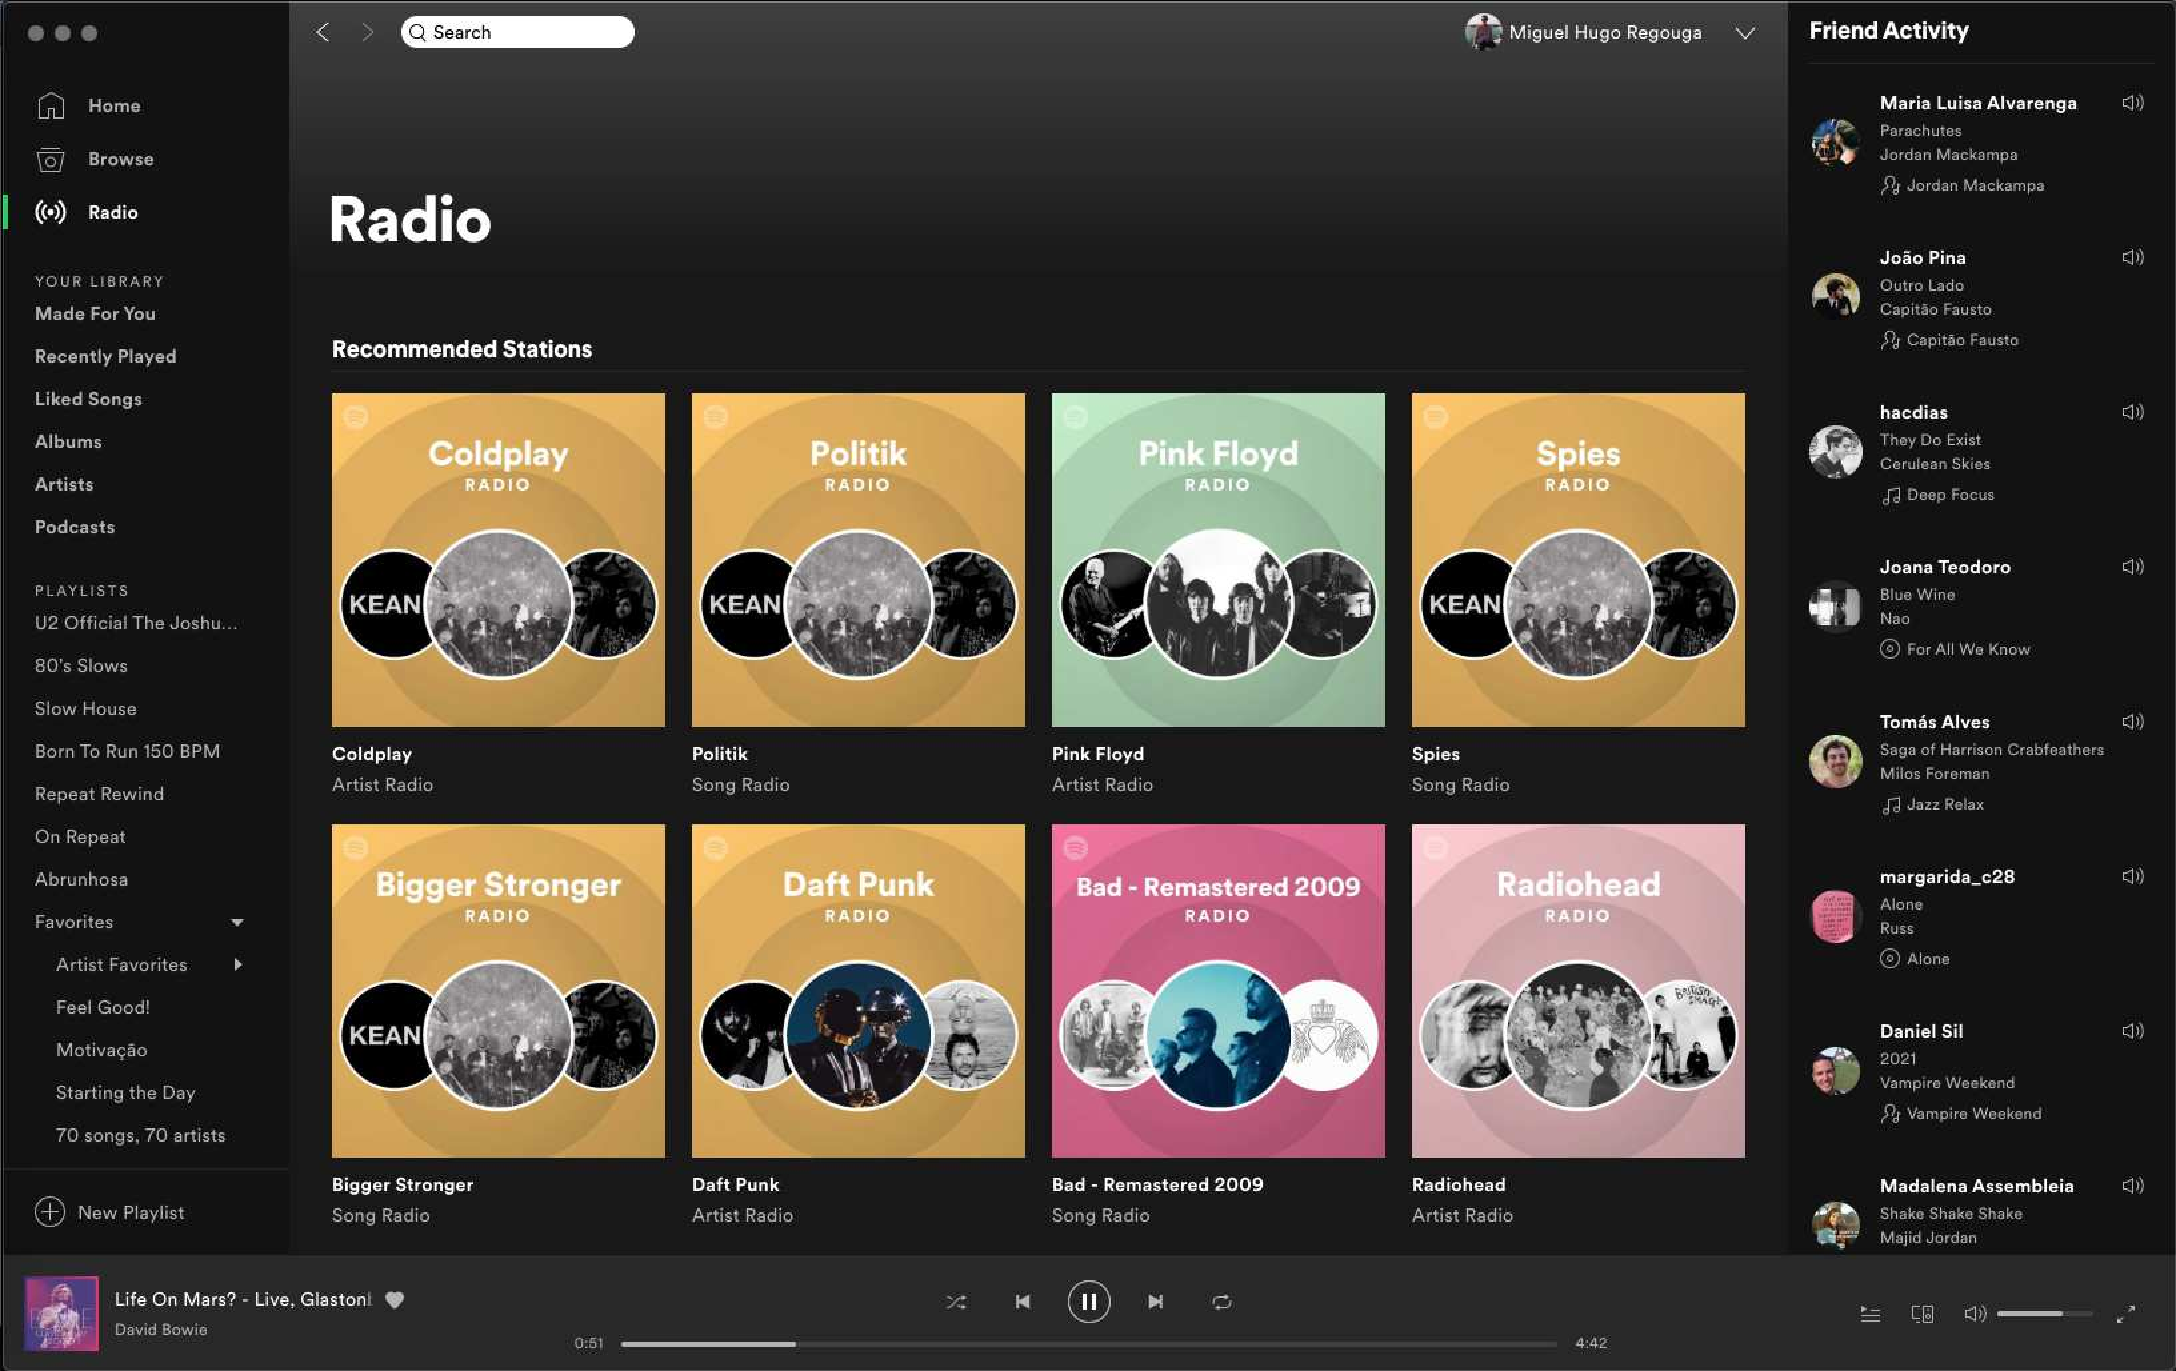
\includegraphics[width=0.8\textwidth]{./Images/spotify.png}
\caption{Spotify 'Radio' discovery features on its desktop application}
\label{fig:test_env}
\end{figure}

Ultimately, the most relevant aspect in the context of our research was Spotify's sociability features. Users can choose from a wide range of playlists created by the Spotify community with hand-picked songs, and not by an algorithm. Furthermore, it is possible to see what friends and family are currently listening to. As Wang et. al ~\cite{Wang2014} described, users of these platforms can be driven by a sense of online community and may be willing to have more interaction with others, and this emphasis on sociability from the inception of the platform might be one of the reasons why it is so popular.

In the context of this project, we consider Spotify as a solid starting point for further analysis and study. It is, according to our criteria, the most solid and robust streaming service available, but has its flaws. As Gunawardena et. al ~\cite{Gunawardena1997} mentions, users can perceive a feeling of warmth and human contact by means of social presence, and although they exist, we find the social features of Spotify quite limited and not enough to provide users a well founded human connection. We'll explore this matter in section ~\ref{sec:methodology}, when we discuss the conducted user research.

\subsection{Apple Music}

In spite of Spotify being currently the most used music streaming service in the world, Apple Music is growing at a fast pace, as it is now the most used streaming service in the United States.\footnote{As of September 2019, reported by \href{https://www.statista.com/statistics/798125/most-popular-us-music-streaming-services-ranked-by-audience/}{Statista}.} The service was born in 2015 after the company Beats was bought by Apple.

When this service was released to the public, its main selling point was that it was bringing a strong human element to these on-demand services, arguing that "algorithms can't do it alone – you need a human touch"~\footnote{\href{https://www.theguardian.com/technology/2015/jun/09/apple-music-interview-jimmy-iovine-eddy-cue}{Apple Music interview: 'Algorithms can't do it alone – you need a human touch' — The Guardian, 2015}}. Thus, the core features of the service were curated playlists, hand-picked by music experts, and recommendations tailored to the users' music preference, not resorting to algorithms (as Spotify does)~\footnote{\href{https://www.theguardian.com/technology/2015/jun/08/apple-music-streaming-service-wwdc-spotify}{Apple unveils streaming service Apple Music and 24-hour radio stations — The Guardian, 2015}}.

Apple Music was also focused to emphasize on traditional terrestrial radio. Along with the introduction of this service, Apple announced they would be launching the Beats 1 radio station (now renamed to Apple Music 1), which broadcasts live to over 100 countries 24 hours a day, and would feature 'real' radio hosts, such as DJ Zane Lowe~\footnote{\href{https://www.theguardian.com/music/2015/feb/16/zane-lowe-apple-bbc-london-radio1-la}{Zane Lowe on Apple, the BBC and why he’ll miss London — The Guardian, 2015}}. In 2020, Apple expanded this section of the service by adding three more 'real' radio stations that offer not only daily curated playlists of music, but also artist interviews, global exclusives and premieres, and other breaking music news. The idea behind these streaming radio stations is to cater to people who, sometimes, just want to turn on music without having to think about what they want to hear or dig around for a favorite playlist. That was the original promise of terrestrial radio, and Apple believes the formula can still work on modern-day streaming services, as well~\footnote{\href{https://www.theguardian.com/music/2015/feb/16/zane-lowe-apple-bbc-london-radio1-la}{Apple launches Apple Music Radio with a rebranded Beats 1, plus two more stations — TechCrunch, 2020}}.

\begin{figure}[h]
\centering
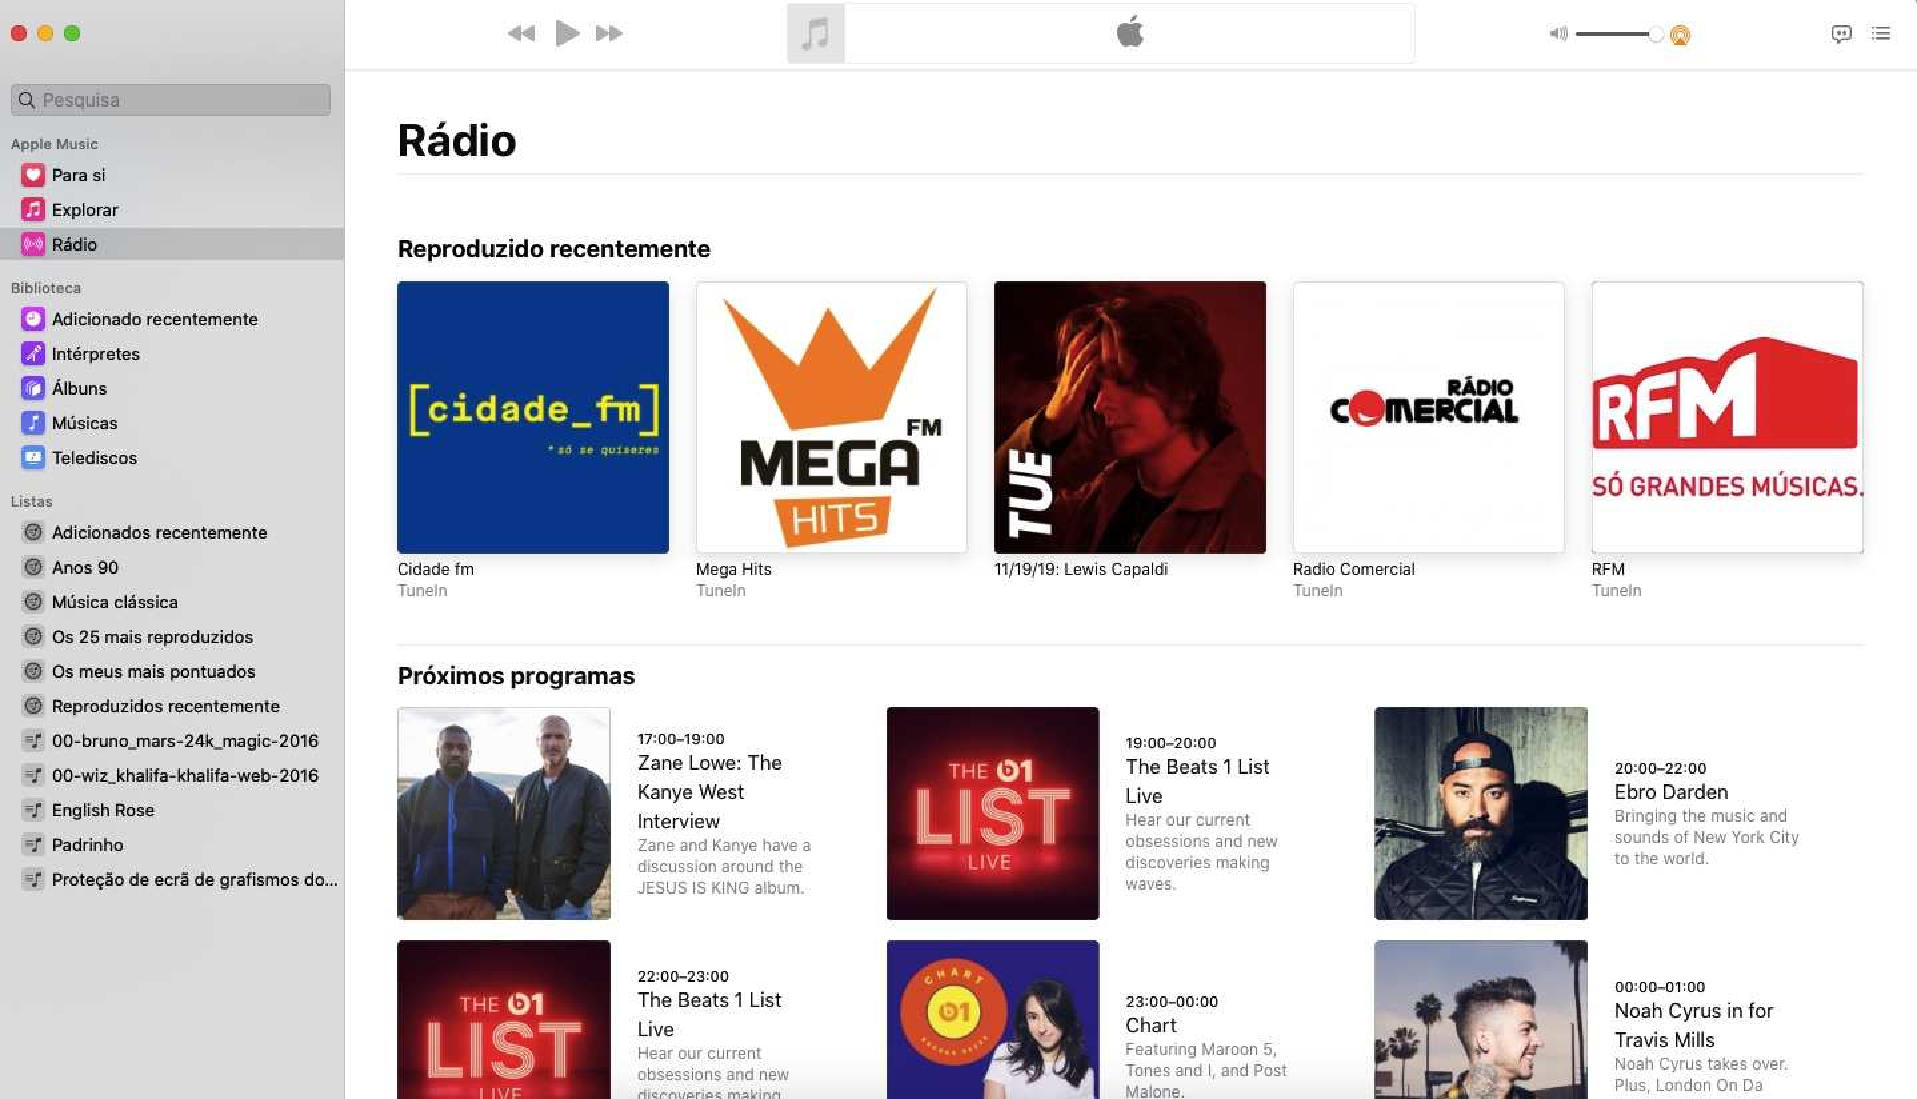
\includegraphics[width=0.8\textwidth]{./Images/applemusic.png}
\caption{Local radio stations and discovery features on the Apple Music 'Radio' tab}
\label{fig:test_env}
\end{figure}

Building on that premise, Apple has also added to the service the ability to search for 'real' radio stations from around the world, allowing users to dial in local broadcast stations by call sign, name, or frequency ~\footnote{\href{https://www.broadbandtvnews.com/2019/09/25/tunein-brings-over-100000-radio-stations-to-apple-music/}{TuneIn brings over 100,000 radio stations to Apple Music — Broadband TV News, 2019}}. Furthermore, the "Radio" tab also incorporates the before-mentioned Apple Music 1 station, as well as other radio stations that play genre-specific or artist-related music, depending on the user's preference. Unlike traditional radio services, the radio feature in Apple Music allows users to skip songs, view previously played tracks on the station, as well as to know what songs are playing next.

In terms of sociability, Apple Music is lacking in features, specially in comparison with Spotify. Although its original release included a 'Connect' screen aimed at creating a social experience between listeners and artists, such feature was later removed due to its low usage~\footnote{\href{https://www.theverge.com/2018/12/13/18139837/apple-music-connect-social-network-feature-discontinued}{Apple is shutting down Apple Music’s rarely-used Connect feature — The Verge, 2018}}. Nevertheless, until 2018, a truly social experience between the platform's users never existed. The ability for users to share what they're listening with their friends was later added~\footnote{\href{https://www.theverge.com/2017/6/5/15727014/apple-music-app-update-social-features-wwdc-2017}{Apple Music will let you share what you’re listening to with your friends — The Verge, 2017}}, yet it is not as developed nor integrated in the platform as Spotify's matching features are.

The approach Apple Music takes on traditional terrestrial radio is very interesting in the ambit of this project. The addition of 'real' radio stations to the service and the commitment to add the option to listen to terrestrial radio stations may prove that users still want to indulge on this medium, despite the convenience that on-demand music selection provides them. Later on the study, we'll analyze the possible reasons why this is happening.

\subsection{Pandora Radio}

The Pandora Radio project was born in 2000, and it is considered one of the oldest streaming services available. The platform is widely popular in the United States, which is the only country it operates in.

Pandora takes on a different approach than the one from Spotify and Apple Music. While both these services were built on an on-demand philosophy, allowing the user to select their desired musical content to play, Pandora wasn't. Pandora enables the creation of 'personal radio stations', in which the user is prompted to choose a song, artist, or album, and a radio station is generated based on that choice (much like the Spotify's own 'radio' feature). ~\cite{Meneses2012} In short, listeners can tune into established genre stations, other users' stations, or create their own stations based on their musical interests. It functions in a similar way to a traditional radio station except that users select a song or artist they want to hear and a station is generated based upon such selection. ~\cite{Swanson2013}

\begin{figure}[h]
\centering
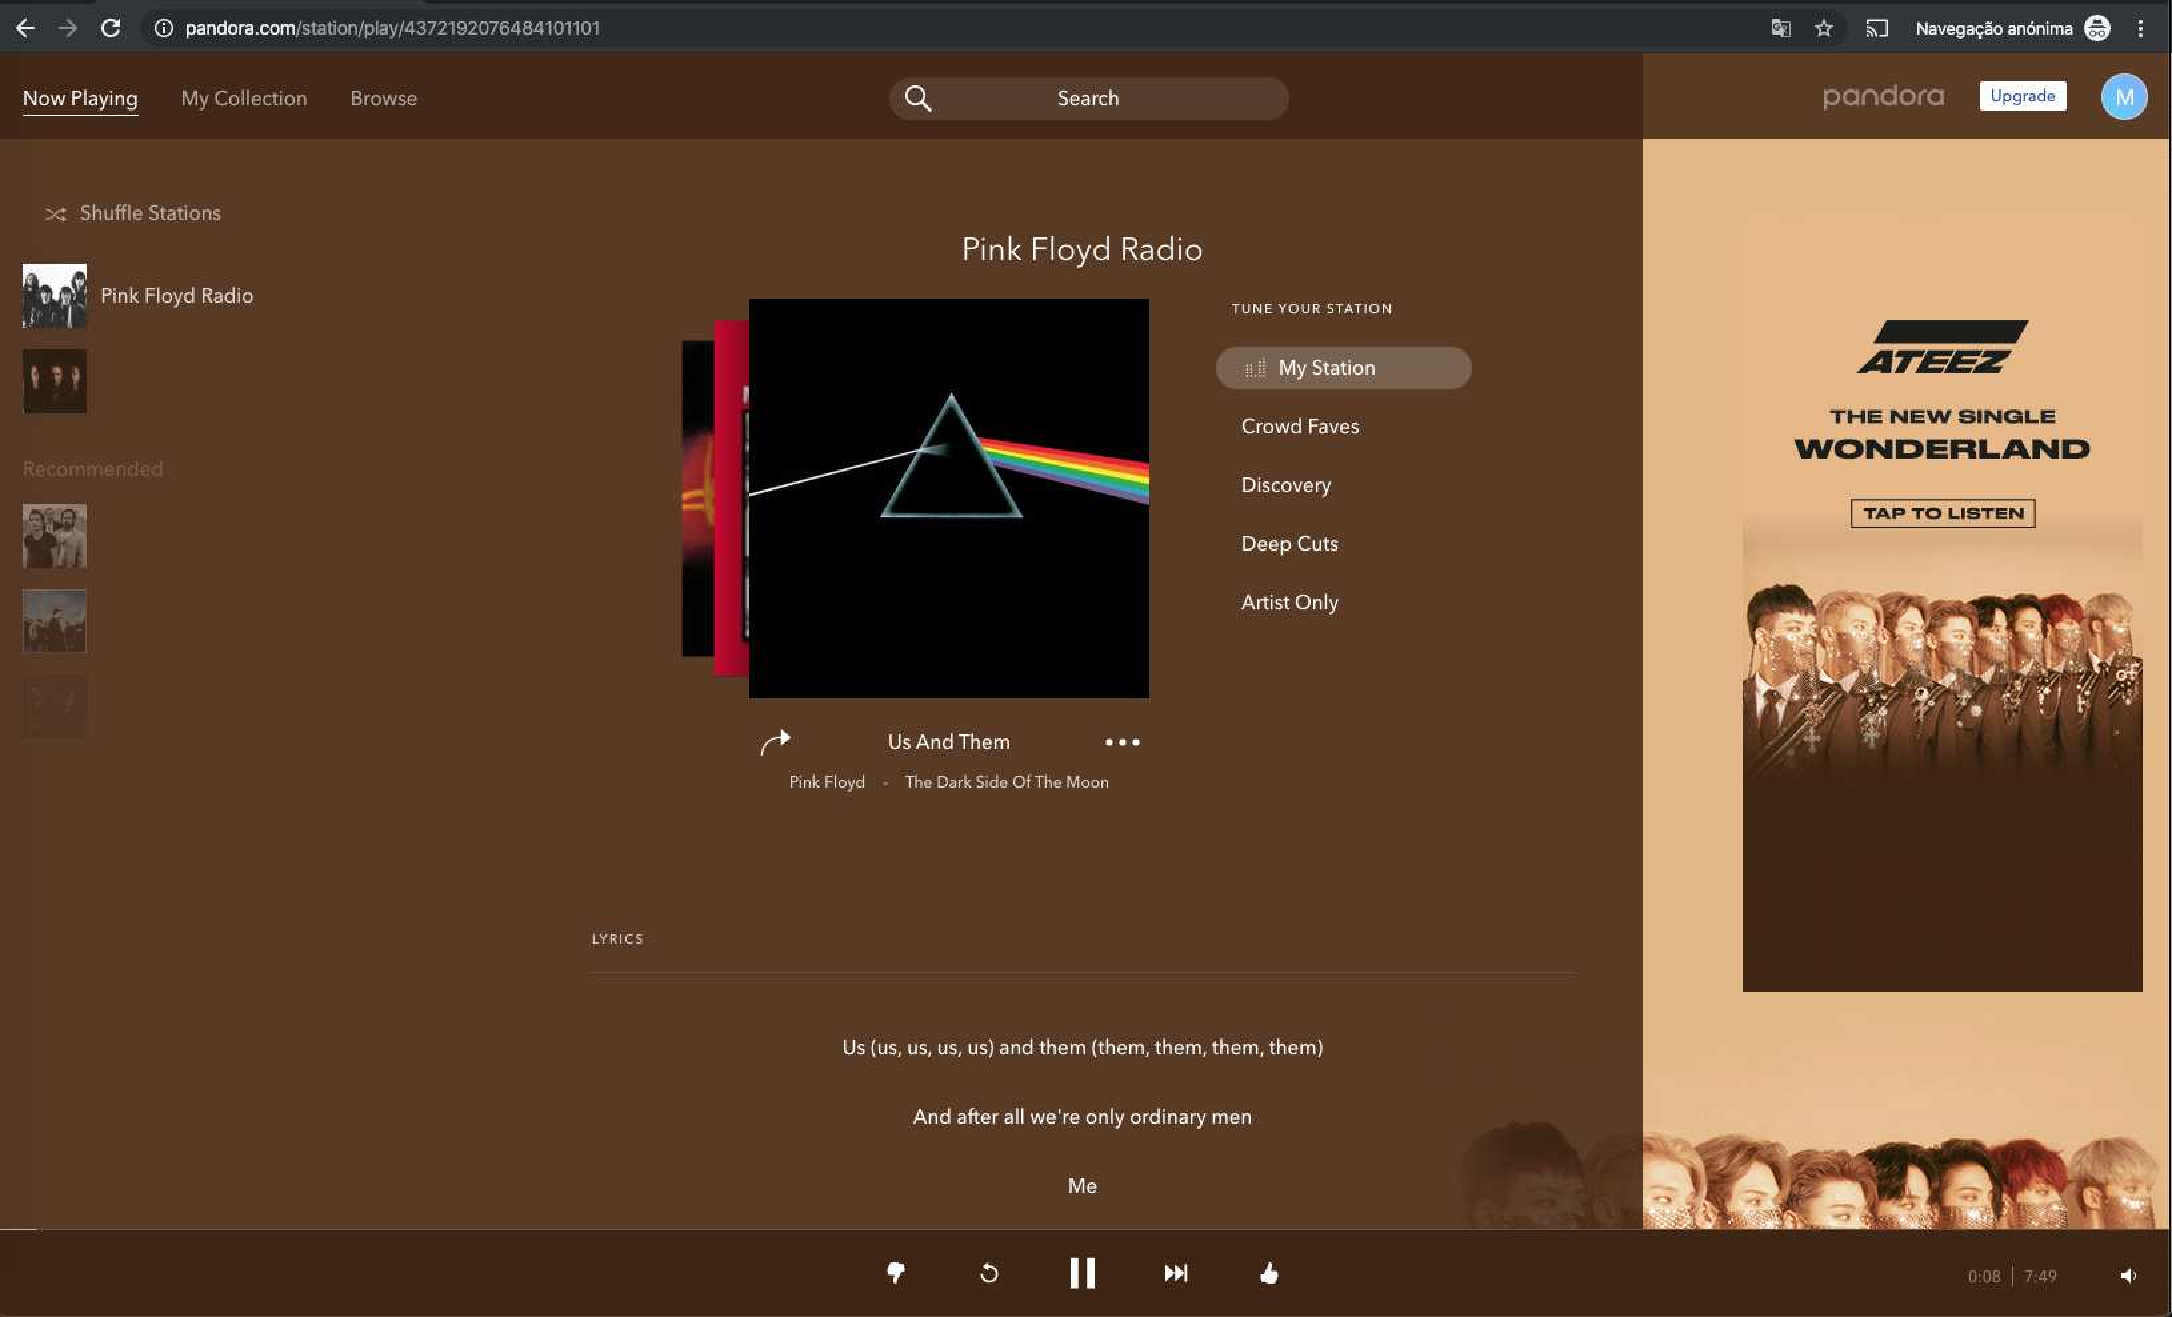
\includegraphics[width=0.8\textwidth]{./Images/pandora.png}
\caption{Pandora Radio web interface}
\label{fig:test_env}
\end{figure}

While listening, users can rate positively or negatively the songs that are being played, and such feedback is taken into account in the subsequent selection of other songs to play, tuning in each station to the users' taste. Furthermore, users may even tailor their station to specific tendencies, such as 'Discovery', 'Crowd Faves', or 'Deep Cuts'.

When talking sociability, Pandora offers the same basic social functionalities as Apple Music — it is possible to follow users, see what they are listening to, and share stations with the community, but the platform isn't as community-centered as Spotify is.

One of the reasons Pandora may be so widely used is the fact that users don't want to choose what they want to listen to all the time. As Meneses mentioned ~\cite{Meneses2012}, having millions of songs available is perfect when users want to listen to the music they are already familiar with, but most users don't want to listen to the same music constantly - hence the creation of discovery features on Spotify and Apple Music. On the other hand, if traditional radio is the main information source on new music, that happens because users want to uncover new material from artists or genres.

%\subsection{Analysis}
%%Tabela comparativa dos music streaming services
%
%Audio streaming services are used daily by millions worldwide, enabling on-demand listening and the discovery of songs, artists and podcasts that closely align with the listener’s preferences. Around the world, there are more than 30 of these platforms available, but the most used ones are Spotify, Apple Music, and Pandora Radio.
%
%Each one of these services offers a unique and enticing set of features to their users. To facilitate the comparison between each service's functionalities, Table ~\ref{tab:mssfeatures} was created, with the lines showcasing the before-mentioned three most popular music streaming services, and the columns showing some cross-cut features of these services, which are:
%
%\begin{itemize}
%\item (a) On-demand music selection
%\item (b) ‘Real’ radio stations
%\item (c) Song discovery features
%\item (d) Shared playlists
%\item (e) Social feeds
%\item (f) Group listening
%\end{itemize}
%
%These functionalities were selected as we consider them to be the most relevant and prominent in the ambit of our case study. 
%
%By analyzing the table, we can conclude that, at a first glance, Spotify is the most robust service of the three, while Pandora Radio is the most limited one. All three services have a very limited set of social features — most importantly, they all lack a true social feed functionality. Although Spotify does offer a 'listening activity' feature, where users can follow and see what other users are listening to, this feature is very limited as it is only available on the desktop counterpart of the service
%
%\begin{table}[]
%\centering
%\resizebox{0.8\textwidth}{!}{%
%\begin{tabular}{|l|c|c|c|c|c|c|}
%\hline
%              & (a)                         & (b)                         & (c)                                                & (d)                         & (e)                        & (f)                         \\ \hline
%Spotify       & \cellcolor[HTML]{34FF34}Yes & \cellcolor[HTML]{FFCCC9}No  & \cellcolor[HTML]{34FF34}{\color[HTML]{333333} Yes} & \cellcolor[HTML]{34FF34}Yes & \cellcolor[HTML]{FFCCC9}No & \cellcolor[HTML]{34FF34}Yes \\ \hline
%Apple Music   & \cellcolor[HTML]{34FF34}Yes & \cellcolor[HTML]{34FF34}Yes & \cellcolor[HTML]{34FF34}Yes                        & \cellcolor[HTML]{FFCCC9}No  & \cellcolor[HTML]{FFCCC9}No & \cellcolor[HTML]{FFCCC9}No  \\ \hline
%Pandora Radio & \cellcolor[HTML]{FFCCC9}No  & \cellcolor[HTML]{FFCCC9}No  & \cellcolor[HTML]{34FF34}Yes                        & \cellcolor[HTML]{FFCCC9}No  & \cellcolor[HTML]{FFCCC9}No & \cellcolor[HTML]{FFCCC9}No  \\ \hline
%\end{tabular}%
%}
%\caption{Summary of the analyzed music streaming services' features}
%\label{tab:mssfeatures}
%\end{table}



\section{Traditional Terrestrial Radio}
\label{chap:ttr}
Radio is the first mass medium that enables the instant dissemination of information from one to many, and it is often described as a "local" and "personable" medium to its audience ~\cite{Ren2004}. It is largely a one-way communication system that allows individual listeners to passively consume radio content provided by radio broadcasters without any interaction or participation ~\cite{Gazi2011}. From its inception, traditional terrestrial radio has been challenged by several innovative technologies, each drawing listeners and forcing radio to update its programming to remain a competitive media option ~\cite{Albarran2007}. 

\begin{figure}
 \centering
	\begin{tikzpicture}
\begin{axis}[
    symbolic x coords={2015,2016,2017,2018,2019},
    xtick=data]
    \addplot[ybar,fill=blue] coordinates {
        (2015,111)
        (2016,112)
        (2017,111)
        (2018,106)
        (2019,102)
    };
\end{axis}
\end{tikzpicture}
\caption{Average daily time spent listening to the radio per adult in the United States (in minutes) —  Statista}
\label{fig:test_env}
\end{figure}


Although music plays a vital role in radio diffusion, traditional terrestrial radio also provides its listeners with useful information, such as news, weather, and traffic reports. A study conducted by Albarran et. al ~\cite{Albarran2007} has shown that, when taking all other audible mediums available into account (including music streaming services), traditional radio is still ranked as the first go-to solution when a user wants to access news and other types of information. 


Waits et. al ~\cite{Waits2007} states that traditional radio still features one of the things that on-demand streaming services may arguably be taking away from its users — a human connection, stating that the users' relationship to this medium is determined by a certain expectation that it will be authentic, sociable, and display intentionally and sincerity. Priestman et. al ~\cite{Priestman2005} argues that the same cannot be said about music streaming services, naming these platforms as 'automated music channels' or 'automated web jukeboxes', due to the absence of the sociable component in conjunction with the emphasis on the listener's music selection. The researchers' approach on traditional radio can be defined as a 'human communication', where one senses that the voice of an announcer creating the threads between various other broadcast elements becomes a key point. 

A different study, conducted by Glantz et. al ~\cite{Glantz2016}, states that, as advanced as music streaming platforms can be, they still anchor themselves in traditional radio. Many of these services market themselves as a "personalized radio", "your radio station", or as far as "radio reimagined". They want their users to believe that they are similar to, but ultimately different from, or better than, traditional terrestrial radio. In contrast, Priestman et. al ~\cite{Priestman2005} describe streaming services as a contradictory phenomenon to define in radio terms, since "it is quite clearly an extension of music format radio but, in doing away with any form of presenter or news or indeed any kind of radio studio at all, it removes the essential element of broadcast communication: one human person talking directly to another or sharing with them some form of entertainment."

In a study conducted in 2008 by Ala-Fossi et. al ~\cite{Ala-Fossi2008}. a group of users predicted that that the numbers of FM radio stations and their listeners would be decreasing by 2015, due to the impact of the emerging internet services, such as music streaming platforms. Yet, in defiance of the competition, traditional radio remains the biggest mass-reach medium in the United States, with more than 90\% of consumers listening on a weekly basis ~\footnote{\href{https://qz.com/195349/the-remarkable-resilience-of-old-fashioned-radio-in-the-us/}{The remarkable resilience of old-fashioned radio in the US — Quartz, 2014}}. The main thesis on why this is happening has to do with the conjunction of two concepts: passive listening, to which traditional terrestrial radio is built upon on; and tyranny of choice. ~\footnote{\href{https://qz.com/1094963/radio-survived-the-tape-cd-and-ipod-in-the-age-of-spotify-its-more-popular-than-ever/}{Radio survived the tape, CD, and iPod. In the age of Spotify, it’s more popular than ever. — Quartz, 2017}} According to Miller, “the availability of so much music has led to what some academics and analysts call the tyranny of choice". Users of music streaming platforms are often hit by this tyranny of choice, where the amount of selection available makes them unable to decide what to listen to, tuning to a 'traditional' radio station where a radio host interacts passively with its listeners. ~\cite{Pedersen2014}.

In short, terrestrial radio still remains with a strong adoption, in spite of the rise of on-demand services. The disclosure of information, the passive audio listening experience, the sense of community, or the human connection that terrestrial radio stations provide may be some of the reasons why users still indulge heavily on this traditional medium. Nevertheless, music streaming services are still rising in popularity, which proves that the convenience of on-demand listening is evident among its users. The concept of interactive radio, which will be discussed in the following section, may provide a hint at a solution that aims to pick on the passive experience of traditional radio and merge it with the on-demand music selection that streaming services provide.

\section{Interactive Radio}

\subsection{Calm Computing}

In 1991, Weiser and Brown suggested that “if computers are everywhere they better stay out of the way, and that means designing them so that the people being shared by the computers remain serene and in control.” ~\cite{Weiser1997} Weiser and Brown’s vision was not realised, as nowadays computers are everywhere, but they do not stay out of our way. Mobile computing is predominantly stop-and-interact and the web demands our constant engagement. Yet, there might be a platform available for a pervasive service that could advance Weiser and Brown’s vision of calm computing: the format of radio.

Audio is an example of content which we can selectively attend to. Many times users listen to music while they do something else: work, run, drive, etc. Vazquez-Alvarez et. al ~\cite{Vazquez-Alvarez2011} showed that, when designing audio interfaces, there was a significant difference between the user experience of selective attention (where audio was in the background and not requiring the full attention of the user) and divided attention (when two audio streams where competing for the user’s attention). This ability for audio to shift between the center of our attention and its periphery fulfills a key element of Weiser and Brown’s vision of calm computing.~\cite{Weiser1997} Calm computing argues that systems should remain in the periphery of our attention until we require their services, at which point they would move to the center of our attention for direct interaction.

Radio is so common as a passive medium that it requires a conceptual leap to regard radio as a possible platform for eyes-free interaction. Yet, similar to interactive television, the concept of interactive radio is not a recent one. Although radio is considered to be a one-way communication channel from station to listener, many radio hosts try to mitigate this by asking listeners to interact with them — either through more analog types of communication, such as phone calls, or using modern platforms such as WhatsApp, enabling the listener to interact more easily with radio stations, potentially augmenting the overall experience of the listener. ~\cite{Claes2018, Ren2004} Yet, in the prime age of social interaction, many researchers have studied how this concept may be taken even further.

\subsection{Nomadic Radio}

One of the first approaches to this concept was presented by Sawhney et. al ~\cite{Sawhney1999} in 1999. The researchers developed a system called \textit{Nomadic Radio} in which scaleable auditory techniques and contextual notification modules for providing timely information were applied, while minimizing interruptions.

\begin{figure}[h]
\centering
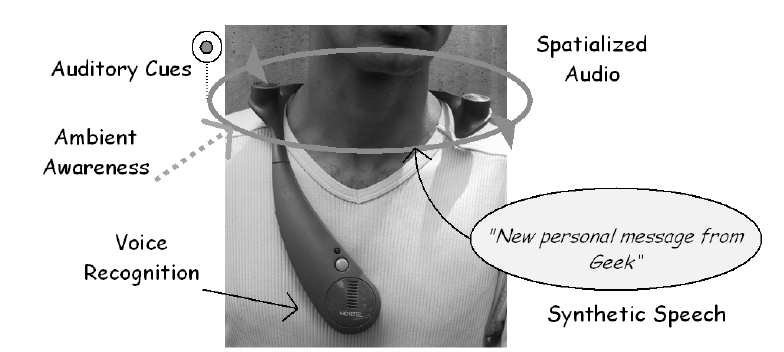
\includegraphics[width=0.8\textwidth]{./Images/nomadicradio.png}
\caption{Description of the Nomadic Radio system with the SoundBeam Neckset audio device}
\label{fig:test_env}
\end{figure}

Nomadic Radio is a wearable computing platform that provided a unified audio-only interface to remote services and messages such as email, voice mail, hourly news broadcasts, and personal calendar events. These messages are automatically downloaded to the device throughout the day and users can browse through them using voice commands and tactile input. This first attempt was, however, targeted at mobile workers rather than at the general audio media consumer.

\subsection{AudioFeeds}

Dingler et. al ~\cite{Dingler2010} built on the \textit{Nomadic Radio} concept and took a more user-centered approach by proposing a mobile auditory display application, called \textit{AudioFeeds}, that allowed users to maintain an overview of activities in different social feeds. The application runs on a mobile device and enables users to get an overview of their social networks and spot peaks in activity by sonifying social feeds and creating a spatialised soundscape around the user’s head. By using this solution, users could stay informed about current issues and spot ‘hot topics’ while on the go. 

\begin{figure}[h]
\centering
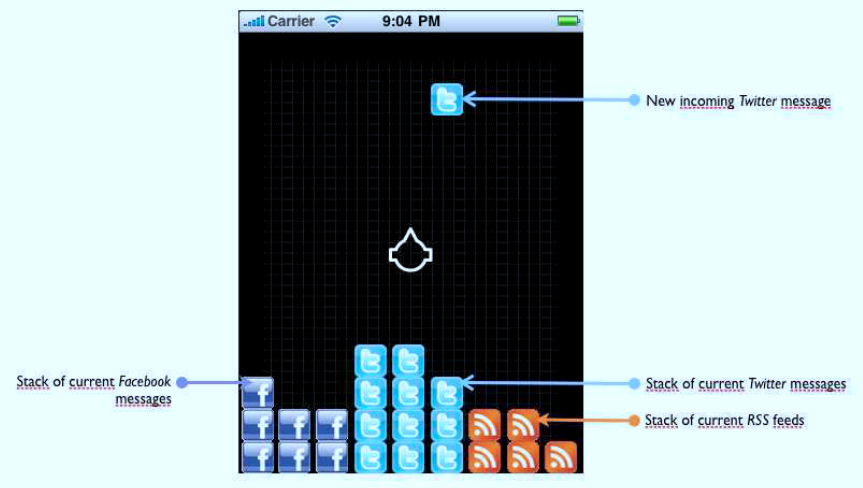
\includegraphics[width=0.8\textwidth]{./Images/audiofeeds.png}
\caption{AudioFeeds GUI, where incoming messages are represented by icons that are dropped from the top}
\label{fig:test_env}
\end{figure}

\textit{AudioFeeds} adapted the idea of adaptive notifications that \textit{Nomadic Radio} introduced and applied it to social feeds and their activity levels. The system enabled users to easily make out interesting social feed activities while maintaining an overview even in complex streams of information, thus fulfilling Weiser’s vision of calm computing~\cite{Weiser1997} and forming a close approximation of a truly interactive radio platform.


\subsection{Radialize}

More recently, Pereira et. al ~\cite{Pereira2013} created a platform for listening to music and radio programs through the Web, allowing the discovery of the content being played by radio stations on the Web, either by managing explicit information made available by those stations or by means of our technology for automatic recognition of audio content in a stream. Users can search, receive recommendations, and provide feedback on artists and songs being played in traditional radio stations, either explicitly or implicitly, in order to compose an individual profile.

\textit{Radialize} utilizes every user interaction as a data source, as well as the similarity abstraction extracted out of the radios’ musical programs, making use of the wisdom of crowds implicitly present in the radio programs. The system was one of the first user-available platforms that introduced a novel social listening experience based on the radio format, aiming to "be responsible for the transition of radio stations as a kind of mass media to a kind of social network".~\cite{Pereira2013}


\begin{figure}[h]
\centering
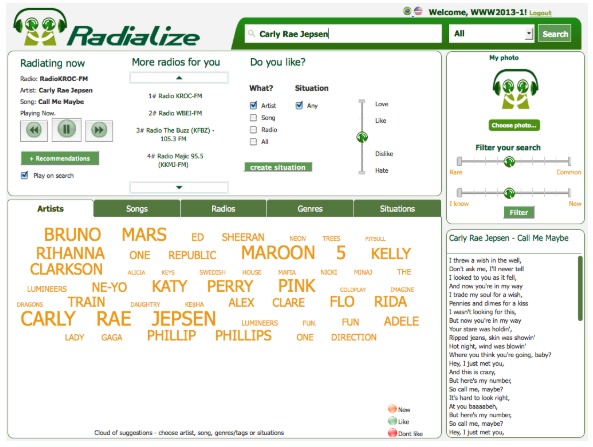
\includegraphics[width=0.8\textwidth]{./Images/radialize.png}
\caption{Screenshot of the Radialize system}
\label{fig:test_env}
\end{figure}

\subsection{MyMyRadio}

Finally, and most importantly, the CereProc team created a platform which takes updates from a user's Facebook or Twitter accounts, and RSS feeds, and synthesizes them using CereProc's own text to speech technology, slotting these spoken updates into a playlist of your own music periodically. ~\footnote{\href{https://www.cereproc.com/en/mymyradio}{MyMyRadio (https://www.cereproc.com/en/mymyradio)}} Aylett et. al~\cite{Aylett2015} have presented a case study on this platform, in which they highlight the potential and challenges of an interactive radio approach, which are of interest to the development of this project.

The MyMyRadio project was developed as a 'cure' to the constant engagement demanded by social networks, enabling content to be delivered in the background while users listened to music and carried out other activities. When a news or a social media was of interest to the user, the user could embrace a more direct and interactive approach with said content, allowing from an active listening experience. If a social, or news headline was of interest, the user would attend to it more closely and could interact directly with the content, moving from a passive or push-down consumption of content to an active or pull-down consumption.

This is in contrast with systems which use audio as notification of content, such as the previously discussed \textit{Nomadic Radio} and \textit{AudioFeeds}, where an audio notification interrupts the current activity. Instead, MyMyRadio inserts content naturally between music tracks to allow continued attention in the periphery. Furthermore, an audio notification system typically does not render the actual information, whereas MyMyRadio uses speech synthesis to render the headline so that only content which is of interest to users is brought to their attention. According to the testing results, the concept of this platform was well received and considered 'desirable' by its users.

\begin{figure}[h]
\centering
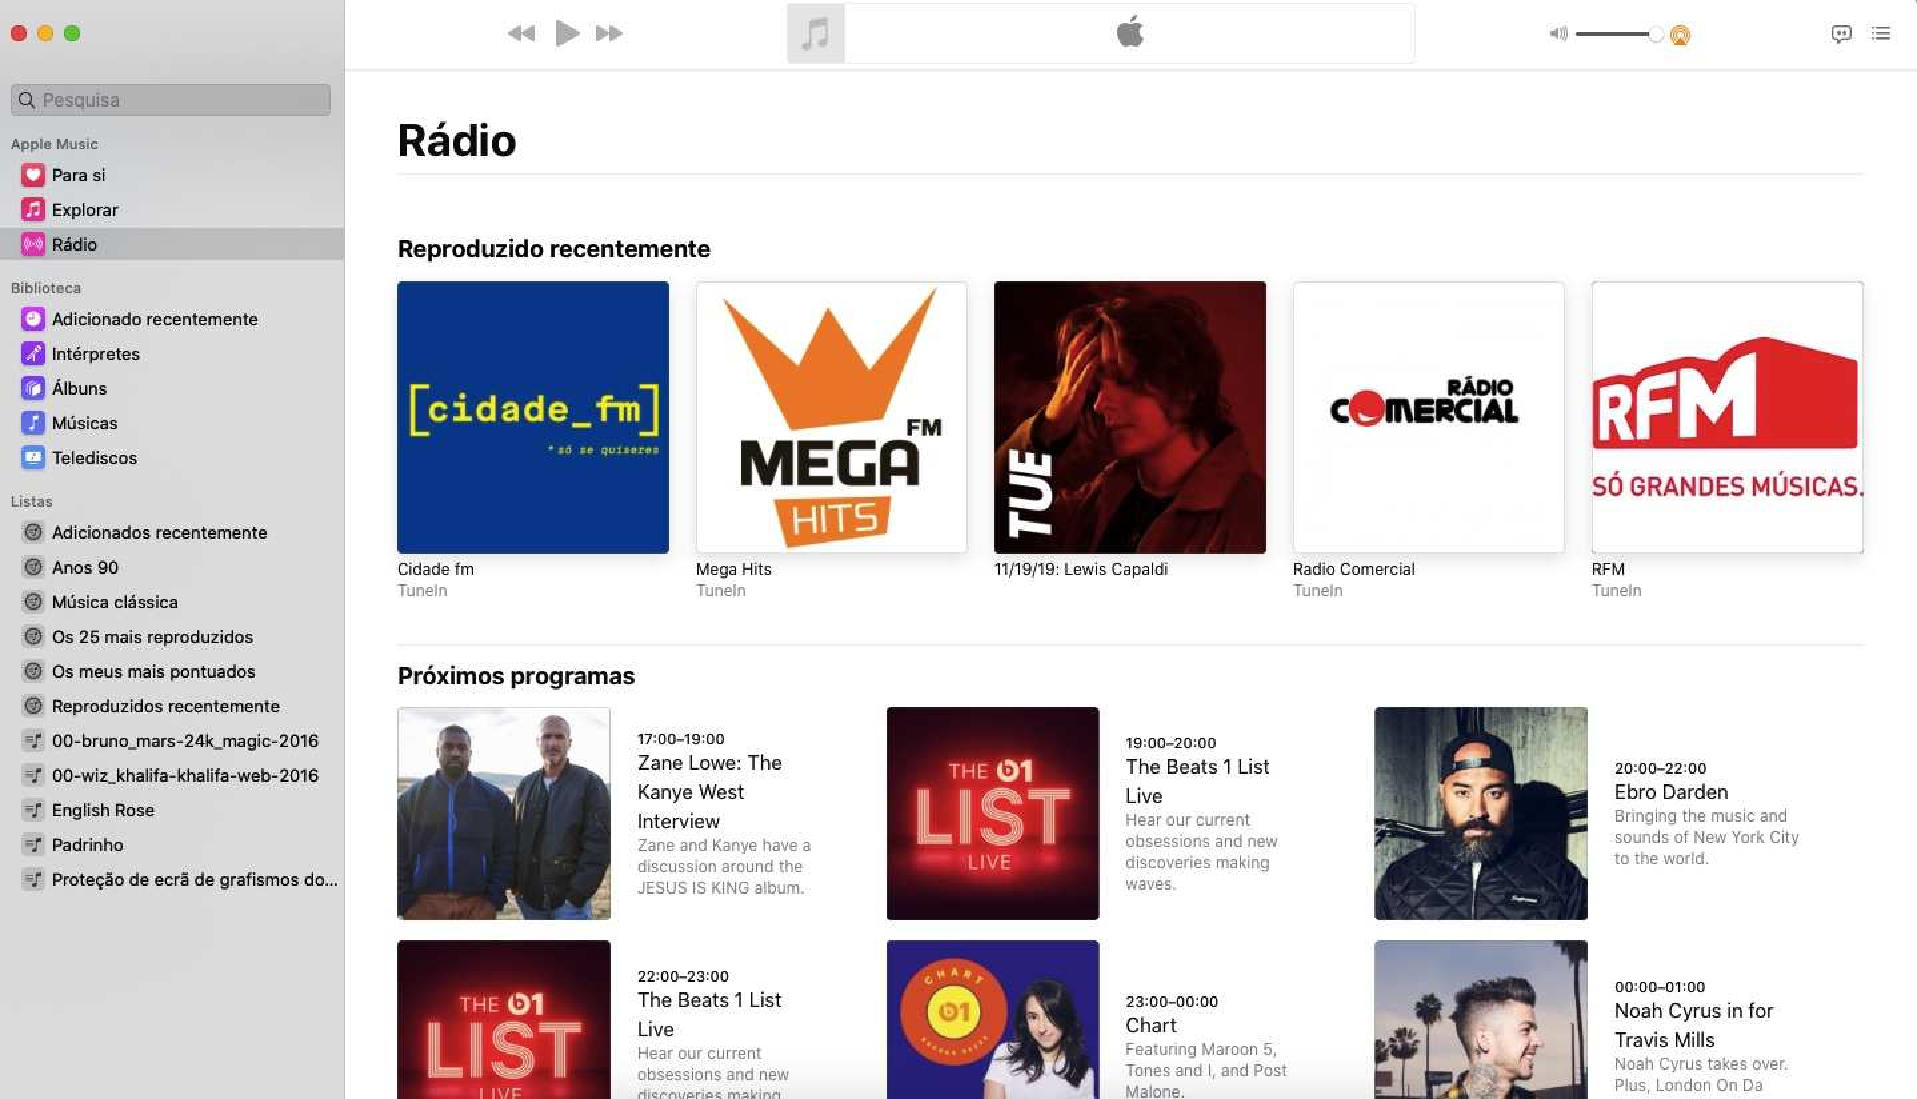
\includegraphics[width=0.8\textwidth]{./Images/applemusic.png}
\caption{MyMyRadio mobile interface}
\label{fig:test_env}
\end{figure}

In the ambit of such case study, the researchers concluded that \textit{'a more developed interactive radio platform could contain localization information and allow a mixture of localized content, speech synthesis and pre-recorded audio, as well as personalized music streams such as Spotify (...) and offer integration with social media and new digital services}.'


\subsection{Analysis}
%Tabela comparativa das interative radio

To facilitate the comparison between the mentioned platforms that implement and augment the interactive radio concept, Table ~\ref{tab:irfeatures} was created, with lines representing a given platform and columns showing some common and relevant features. We selected these features because we consider them to be the most important in the ambit of our case study. The mentioned features are:

\begin{enumerate}[label=(\alph*)]
	\item Audio notifications (interrupts current activity);
	\item News and social feeds (RSS, Facebook, Twitter);
	\item Integration with local (offline) music library;
	\item Integration with music streaming services;
	\item Speech synthesis of information (text-to-speech);
	\item On-site information rendering;
	\item Audio effects (adverts, jingles, background music);
	\item Social network/community features;
	\item Customization and recommendations;
\end{enumerate}


\begin{table}[]
\centering
\resizebox{\textwidth}{!}{%
\begin{tabular}{|l|c|c|c|c|c|c|c|c|c|}
\hline
              & (a)                         & (b)                         & (c)                         & (d)                        & (e)                         & (f)                         & (g)                         & (h)                         & (i)                         \\ \hline
Nomadic Radio & \cellcolor[HTML]{9AFF99}Yes & \cellcolor[HTML]{FFCCC9}No  & \cellcolor[HTML]{FFCCC9}No  & \cellcolor[HTML]{FFCCC9}No & \cellcolor[HTML]{FFCCC9}No  & \cellcolor[HTML]{FFCCC9}No  & \cellcolor[HTML]{FFCCC9}No  & \cellcolor[HTML]{FFCCC9}No  & \cellcolor[HTML]{FFCCC9}No  \\ \hline
AudioFeeds    & \cellcolor[HTML]{9AFF99}Yes & \cellcolor[HTML]{9AFF99}Yes & \cellcolor[HTML]{FFCCC9}No  & \cellcolor[HTML]{FFCCC9}No & \cellcolor[HTML]{FFCCC9}No  & \cellcolor[HTML]{FFCCC9}No  & \cellcolor[HTML]{FFCCC9}No  & \cellcolor[HTML]{FFCCC9}No  & \cellcolor[HTML]{FFCCC9}No  \\ \hline
Radialize     & \cellcolor[HTML]{FFCCC9}No  & \cellcolor[HTML]{FFCCC9}No  & \cellcolor[HTML]{FFCCC9}No & \cellcolor[HTML]{FFCCC9}No & \cellcolor[HTML]{FFCCC9}No  & \cellcolor[HTML]{FFCCC9}No  & \cellcolor[HTML]{FFCCC9}No  & \cellcolor[HTML]{9AFF99}Yes & \cellcolor[HTML]{9AFF99}Yes \\ \hline
MyMyRadio     & \cellcolor[HTML]{FFCCC9}No  & \cellcolor[HTML]{9AFF99}Yes & \cellcolor[HTML]{9AFF99}Yes  & \cellcolor[HTML]{FFCCC9}No & \cellcolor[HTML]{9AFF99}Yes & \cellcolor[HTML]{9AFF99}Yes & \cellcolor[HTML]{9AFF99}Yes & \cellcolor[HTML]{FFCCC9}No & \cellcolor[HTML]{FFCCC9}No  \\ \hline
\end{tabular}%
}
\caption{Summary of the analyzed interactive radio and calm computing platforms}
\label{tab:irfeatures}
\end{table}

The first feature determines if the system uses audio as notification of content, which interrupts the current activity of the listener ~\cite{Dingler2010}. The MyMyRadio system inserts content naturally between music tracks to allow continued attention in the periphery, which can result in an improved experience for the user.

Regarding the more social features, AudioFeeds and MyMyRadio provide integration with various social networks and news aggregation services, but AudioFeeds does not render the information locally as MyMyRadio does. This gives an advantage to the latter platform, which uses speech synthesis to render the headline so that only content which is of interest to users is brought to their attention. ~\cite{Aylett2015} However, although it aggregates displays content from social networks, MyMyRadio doesn't offer a truly social experience between users of the platform, and this is where Radialize has an advantage over the studied platforms.

By analyzing the table, we can observe that MyMyRadio is the most feature-packed platform, closely aligning with the scope of our project. It features a radio-like experience for its users by including audio dynamically created from news and social media sources, integration with the users' local music library, non-speech audio sound effects, and background music. 

Yet, we can observe that none of the studied platforms offer integration with music streaming services, which, as we discussed in section ~\ref{subchap:mss}, are now one of the preferred mediums for consuming audio content. Furthermore, only one platform offers a truly customizable experience tailored to each individual user, while also indulging them in a social-network like atmosphere. Identifying this will be important for defining our window of opportunity and to determine out how we can create a novel listening experience.

In conclusion, the concept of interactive radio can be further augmented, as, at first sight, there is both a user impulse for this to happen, and an opportunity that we can approach and tackle. Based on our research, this may be achieved by merging the strengths of both traditional terrestrial radio and music streaming services into a personal, yet sharable and customizable platform that aims to improve audio media consumers' listening experience. To assure this need, we'll conduct in-depth user research, aiming at understanding if users find such concept enticing.

% If Printing on DOUBLE SIDED pages, the second page should be white.
% Otherwise, comment the following command:
\cleardoublepage
%
%Chapter 3
% #############################################################################
% This is Chapter 3
% !TEX root = ../main.tex
% #############################################################################
% Change the Name of the Chapter i the following line
\fancychapter{User Research}
\cleardoublepage
% The following line allows to ref this chapter
\label{chap:userresearch}

Before proposing a solution that aims at taking the concept of interactive radio further, we need to assess the need and desirability for such a solution. The before-presented literature identifies a demand; yet, as audio consuming mediums are very user-focused, there is a need to conduct a detailed investigation among these users' habits.

Furthermore, the foundation of this research project is a user-centered design development approach ~\cite{McLoone2010}, as we want our hypothetical solution to suit the user, rather than making the user suit our solution. This is accomplished by employing techniques, processes, and methods, throughout the product life cycle that focus on the user. ~\cite{Courage2005} 

In a user-centered design approach, there are three main principles: an early focus on users and tasks, empirical measurement of usage, and iterative design ~\cite{Courage2005}. In this first stage of the project, we'll focus on the first principle — we want a systematic and structured collection of users’ experiences so that we can maximize the quality of the user experience of our developed solution. By collecting user experiences, we can gain an understanding of what users want and need, how they currently work or how they would like to work, as well as the mental representations of their domain.

To best understand our users' habits and to have them into account from the very early stages, we have used three different user experience research activities: \textbf{survey}, \textbf{diary study}, and \textbf{interviews}. In this section, we describe the applied procedures and efforts of each method, followed by an analysis of all the gathered data.


\section{Survey}
Surveys can be a viable approach to gathering data from a large sample in a moderately brief time frame. ~\cite{Courage2005} They can help identify a target user population, current pain points, and opportunities that a solution could fulfill, and find out at a high level how users are currently accomplishing their tasks. Surveys ask every user the same questions in a structured manner, and participants can complete them in their own time and from the comfort of their home.

In this first stage, we wanted to reach a large number of people, and, according to Courage et al. ~\cite{Courage2005}, surveys are the indicated user research method to fulfill this requirement. Thus, we have conducted a survey, presented in Appendix ~\ref{chapter:appendixA}, using the online tool Google Forms~\footnote{For more information, visit the \href{http://forms.google.com/}{Google Forms website}.}. We started by sharing it among our university’s social groups to obtain a younger age range of respondents. Conversely, to get a set of participants from older age ranges and different socio-economical backgrounds, we also shared the survey among local general-themed social groups. The use of these different channels resulted in a broad set of respondents with distinct ages, occupations, socio-economical backgrounds, and audio media consuming habits. Over one week, we gathered \textbf{195 responses}, where 58.8\% of them come from respondents with ages 30 or below. Corroborating with this age range, half of the respondents are mostly students; the other half are employed.


\begin{figure}[h]
\centering
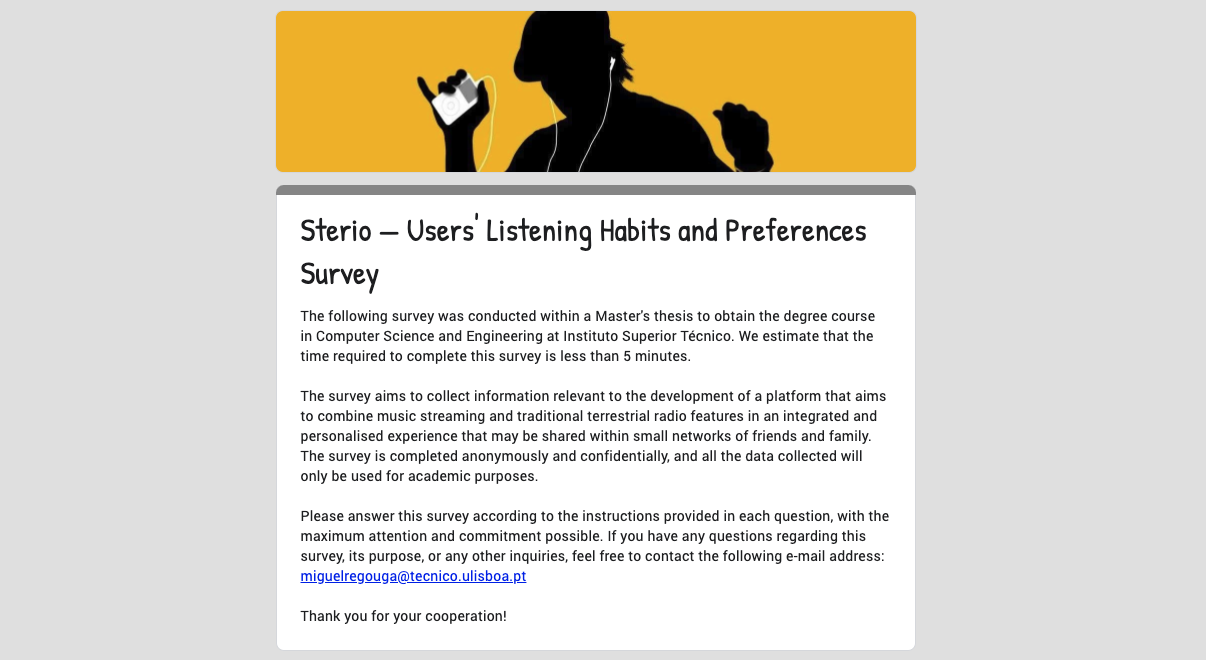
\includegraphics[width=0.8\textwidth]{./Images/survey.png}
\caption{Homepage and introduction to the conducted survey}
\label{fig:test_env}
\end{figure}

Among demographic and other miscellaneous user characterization questions, the following set of queries were asked:

\begin{itemize}
  \item How often do you listen to music?
  \item Which mediums do you use regularly to listen to music?
  \item How often do you use streaming services?
  \item Which music streaming service is your most used one?
  \item On average, how long do you use streaming services in a listening session?
  \item Which of these factors do you consider more relevant when using a streaming service?
  \item What are the factors that stop you from using streaming services on a more regular basis?
  \item Do you listen regularly to podcasts?
  \item How often do you listen to traditional radio stations?
  \item On average, how long do you typically listen to radio?
  \item Where do you usually listen to radio?
  \item What are the main reasons that make you listen to radio stations?
  \item What are the factors that stop you from listening to radio stations on a more regular basis?
\end{itemize}

When asked how often they use music streaming services, only 7\% replied that they don't use them, and \textbf{almost 60\% use them every day}. \textbf{Spotify} is the most used streaming service amongst them, while YouTube (which many use as a means of a streaming service) comes in second place. Users value these services' \textbf{wide range of music selection}, \textbf{sound quality}, and \textbf{low price}, but 16.7\% of them still prefer to use another medium.

\begin{figure}
	\centering
	\caption{Which of these factors do you consider more relevant when using a music streaming service?}
	\begin{bchart}[step=10,max=80,unit=\%,width=0.8\textwidth]
        \bcbar[text=Sound quality]{59.3}
            \smallskip
        \bcbar[text=Wide range of music selection]{71.2}
            \smallskip
        \bcbar[text= Convenience]{68}
            \smallskip
        \bcbar[text=To discover new music]{52.5}
            \smallskip
        \bcbar[text=Curated playlists]{32}
    \end{bchart}
\end{figure}


Regarding traditional terrestrial radio stations, 40.6\% of the inquired listen to them daily, with 5.9\% not listening to this medium at all. Almost half of the inquirers state that the main reason that makes them listen to radio stations is the \textbf{disclosure of news, weather, and traffic information}, with \textbf{convenience} and the \textbf{good mood of the radio hosts} following in second and third places respectively. On the downside, users don't listen to radio more frequently since they believe the music selection is too repetitive (58.2\%) or doesn't fit their taste (40.1\%); due to the high rate of advertisement breaks (50.8\%); and because they can't choose what they want to listen to (38.4\%).

\begin{figure}
	\centering
	\caption{What are the main reasons that make you listen to radio stations?}
	\begin{bchart}[step=10,max=45,unit=\%,width=0.8\textwidth]
        \bcbar[text=Listening to news/weather/traffic information]{41.3}
            \smallskip
        \bcbar[text=Convenience]{37.4}
            \smallskip
        \bcbar[text=Good mood of radio hosts]{33}
            \smallskip
        \bcbar[text=Radio shows]{17.3}
            \smallskip
        \bcbar[text=Other]{11.2}
    \end{bchart}
\end{figure}



\begin{figure}
	\centering
	\caption{What are the factors that stop you from listening to radio stations on a more regular basis?}
	\begin{bchart}[step=10,max=70,unit=\%, width=0.8\textwidth]
        \bcbar[text=Music is too repetitive]{58.1}
            \smallskip
        \bcbar[text=Music does not fit my taste]{40.2}
            \smallskip
        \bcbar[text=Too many ad breaks]{50.8}
            \smallskip
        \bcbar[text=Can't choose what to listen]{38.7}
            \smallskip
        \bcbar[text=Other]{14.6}
    \end{bchart}
\end{figure}


From this first set of gathered data, we can arrive at some early conclusions. The first one is that music streaming services are really popular among this set of users, mainly because they see the advantage of having the possibility on-demand selection of music artists, songs, and genres. However, regarding radio stations, users enjoy the role of the radio host and the disclosure of information this medium provides, but often don't enjoy the music selection nor the long advertisement breaks.

As surveys allow us to reach a larger number of people, the use of this user research method may be a favorable first-step to start user research procedures. To obtain more detailed data about the users' audio media consumption habits, we have also conducted a diary study and interviews, so we could gather qualitative data and cross-reference it with the information obtained through surveying.

\section{Diary study}

To take a deeper look into audio media users' music streaming and traditional terrestrial radio habits, we conducted a diary study, which asks participants to capture information about their activities, habits, thoughts, or opinions as they go about their daily activities. ~\cite{Courage2005} This method allows the collection of typically longitudinal data \textit{in situ}. 

In order to obtain more raw and personal details regarding their audio consuming habits, we involved our own family and friends circle from the very beginning of the project, so we could understand how we can target and improve their experience. As we'll further discuss, we also want to understand how our solution could tackle the social presence and online community concepts, as described by Wang et al. ~\cite{Wang2014}.

We selected 11 close friends and family to conduct a diary study over one week (the participating users on all user research activities are reported in table ~\ref{tab:users}). From these users, 9 are paid subscribers of a music streaming service, while the other 2 use the free tier plan (if available). Users were asked to fill out a template spreadsheet on the Google Sheets~\footnote{For more information, visit the \href{http://sheets.google.com/}{Google Sheets website}.} platform at the end of each day. The template, shown in fig. \ref{fig:diarystudy} and presented in Appendix ~\ref{chapter:appendixB}, had a set of pre-specified questions or probes for users to respond to, making this a structured diary study. Users were asked to sign an informed consent form, presented in Appendix ~\ref{chapter:appendixC}, informing them how their data would be used and the importance of it in regards to the development of our platform.


\begin{figure}[h]
\centering
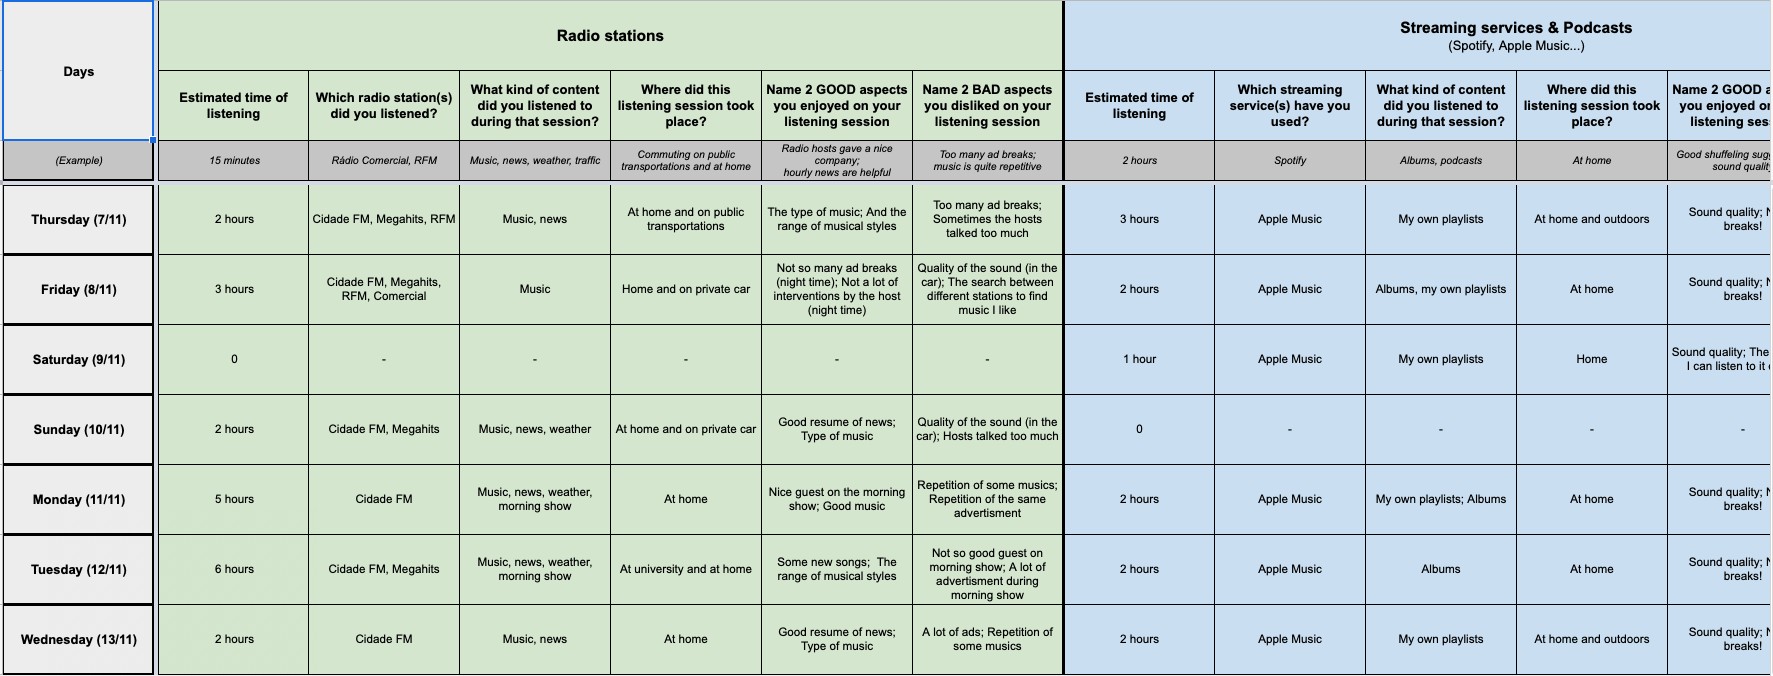
\includegraphics[width=0.8\textwidth]{./Images/diarystudy.png}
\caption{Diary study spreadsheet template filled by one user}
\label{fig:diarystudy}
\end{figure}


The diary study focused on four main audio listening mediums: traditional terrestrial radio stations, music streaming services, music videos, and physical format. Each medium had the following questions:

\begin{itemize}
  \item Estimated time of listening (in minutes);
  \item What kind of content did you listened to during that session?
  \item Where did this listening session took place?
  \item Name two good aspects you enjoyed on your listening session;
  \item Name two bad aspects you disliked on your listening session.
\end{itemize}

From this study, we could analyze both quantitative and qualitative data. Regarding the first, we have concluded that, on average, every user spends more than 3 hours per day listening to various audio content; streaming services count for about 62\% of that, while traditional radio stations count for 21\%. From the 11 users, 2 didn't use music streaming services during that week and are non-paid subscribers, and 3 didn't listen to traditional radio stations in the same period. 

The main outcome of this diary study was, however, qualitative data. For the analysis of such data, we used an \textbf{affinity diagram} ~\cite{Wilson2012}. In an affinity diagram, researchers extract the data from each participant, pulling out key points, and write each note individually on an index card or sticky note~\cite{Courage2005}. Similar findings or concepts are then grouped to identify themes or trends in the data. 

Affinity diagrams can add structure to a large or complicated issue, as they can break it down either into broader categories or more specific, focused categories. This assists and guides designers in the process of identifying issues that affect multiple areas, making affinity diagrams a crucial tool for organizing qualitative data into themes that may offer insights for the design and testing~\cite{Holtzblatt1988}. Figure \ref{fig:diagram1} illustrates the first iteration of the affinity diagram created based on this study's participants' data.

\begin{figure}[h]
\centering
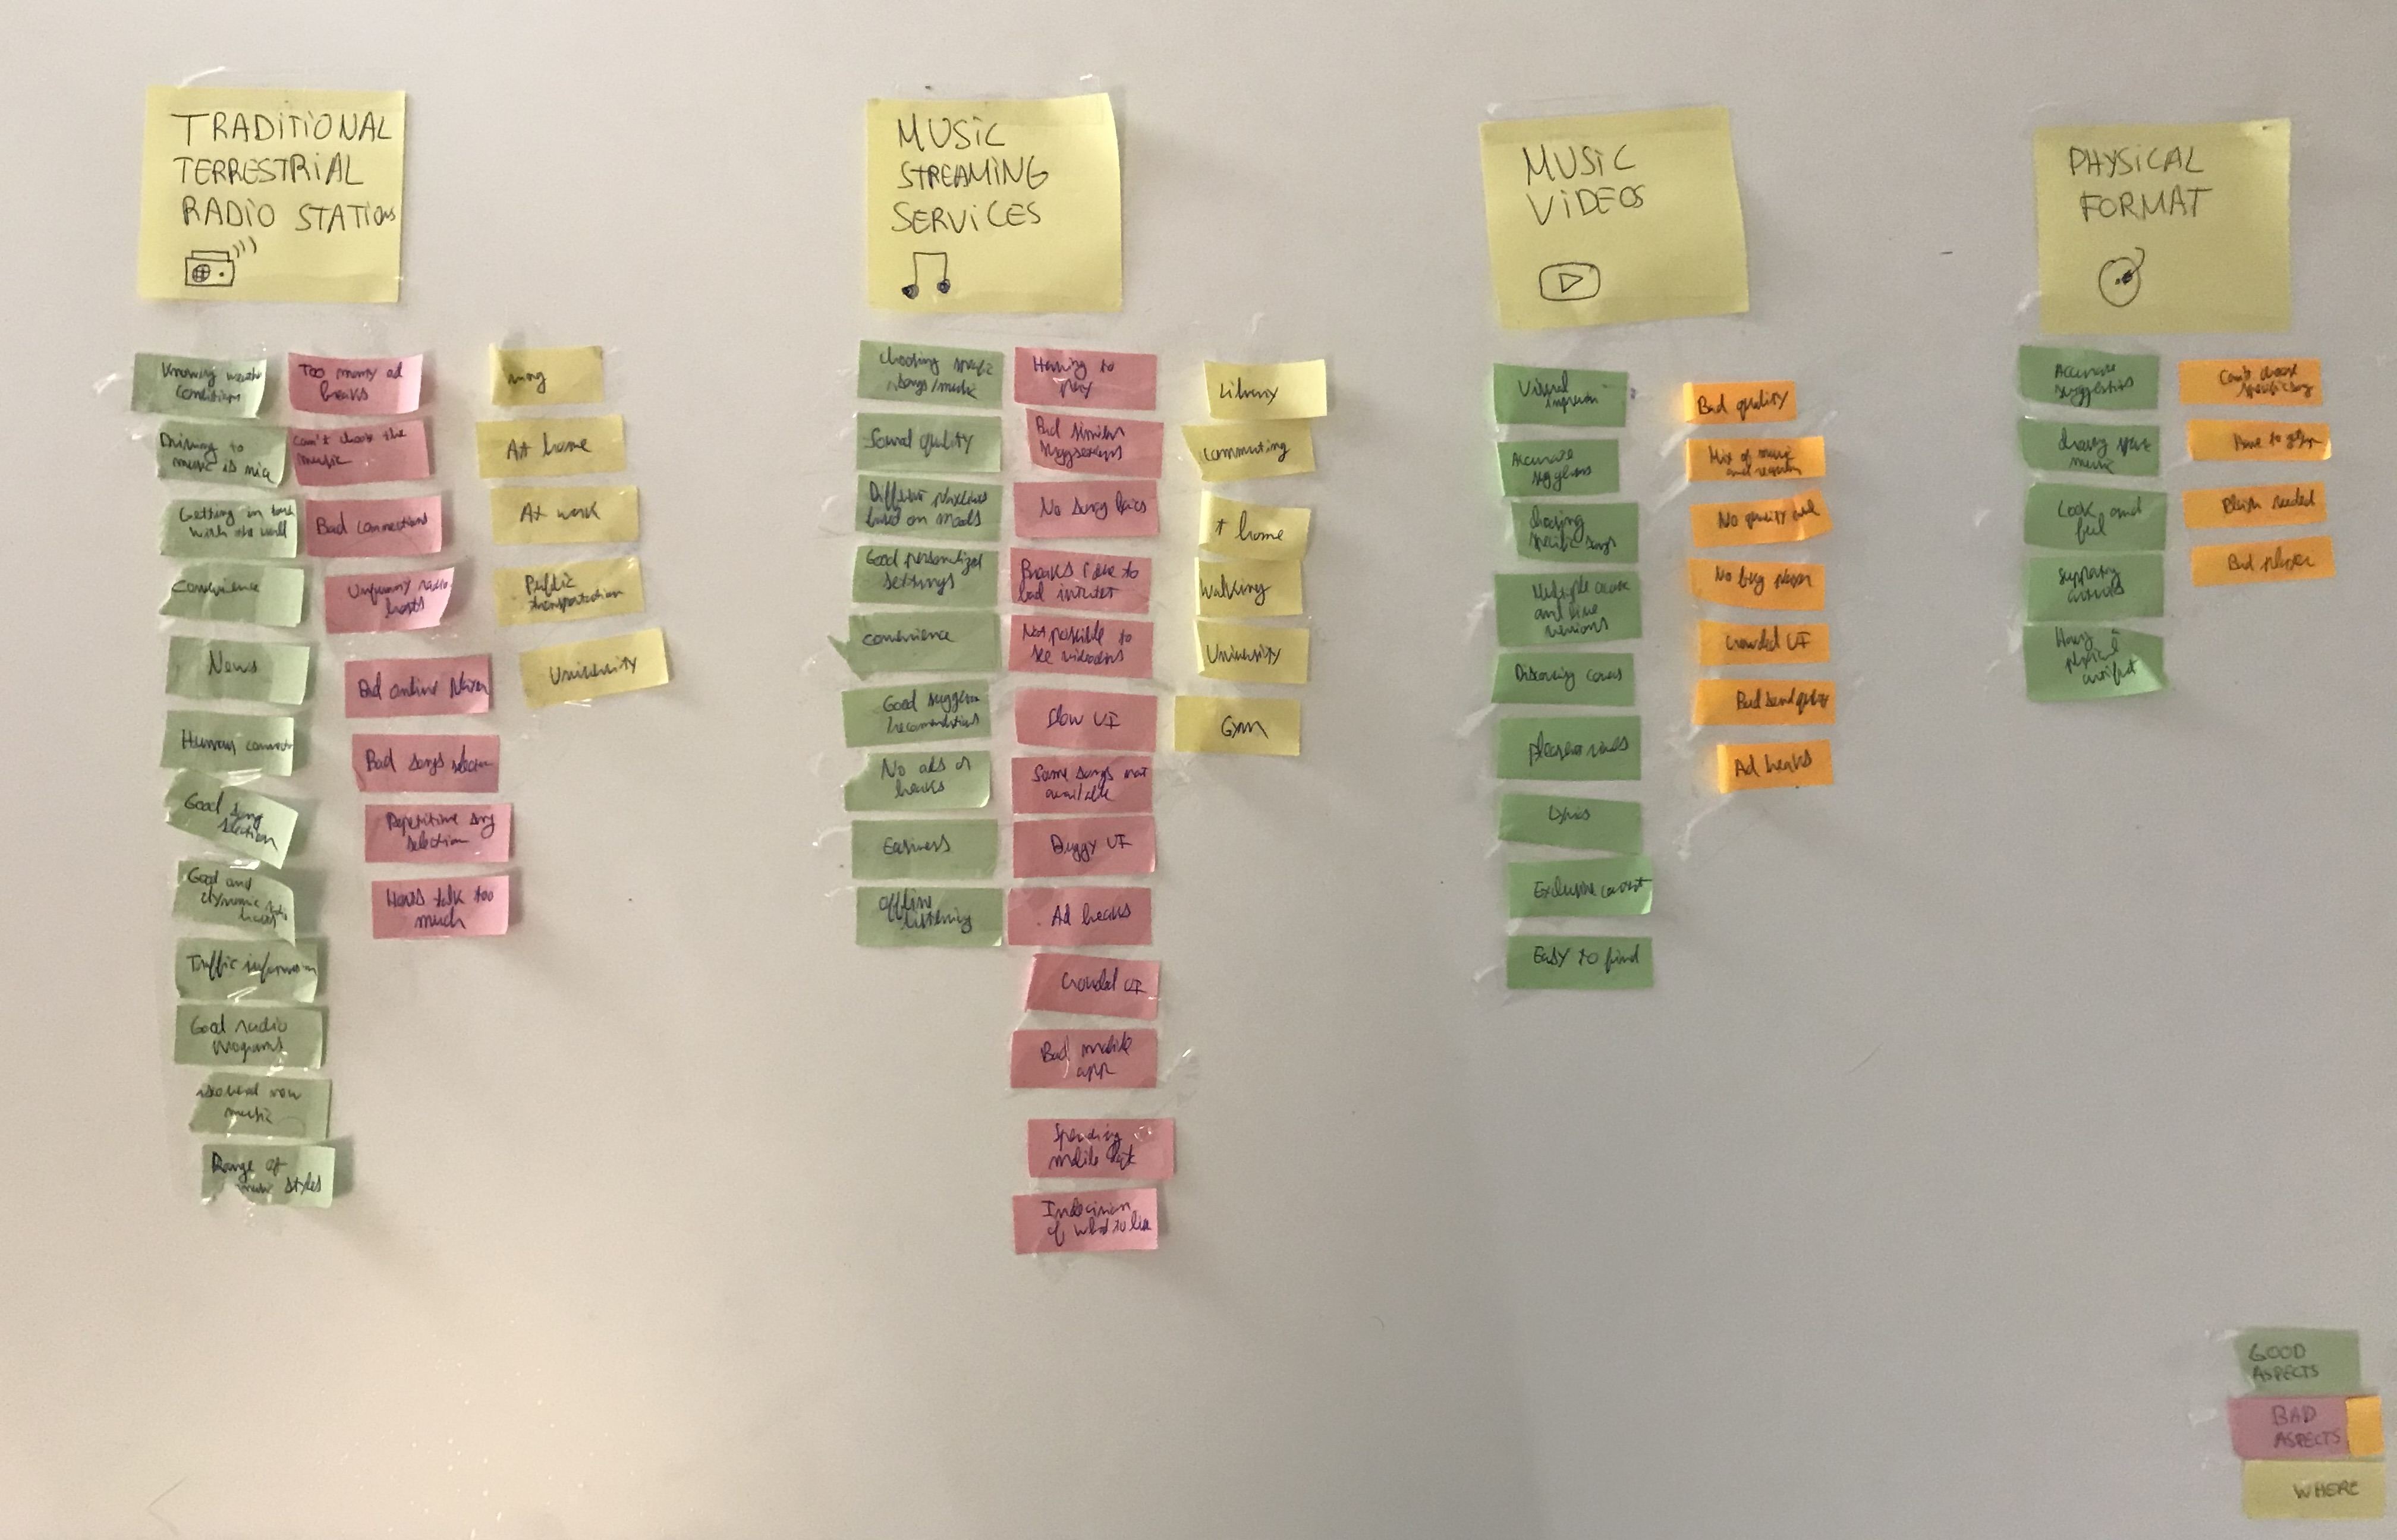
\includegraphics[width=0.8\textwidth]{./Images/affinitydiagram.jpg}
\caption{Affinity diagram with the gathered data from the diary study}
\label{fig:diagram1}
\end{figure}


From the analysis of this data, some conclusions emerged. Regarding traditional terrestrial radio, users enjoy the human connection it provides and the dynamics of the radio hosts. The disclosure of information such as news, weather, and traffic reports is also very important when it comes to listening to radio, as well as the diversity of radio shows that are broadcast. On the downside, most radio listeners of this study don't like the song selection of the stations, as they find it very repetitive, always of the same genre, or simply not matching their musical taste. Not being able to choose what they want to listen to on the radio is something that frustrates them, as well as the amount of radio advertisement breaks.

In contrast, users value the \textbf{freedom of music choice} in music streaming services, as well as its overall \textbf{sound quality} and \textbf{convenience}. They appreciate the \textbf{automatically generated playlists} based on their mood or even their taste. The added freedom that music streaming services provide sometimes isn't a great feature to some users, as they sometimes have indecision of what to listen to (corroborating the tyranny of choice concept discussed in Chapter ~\ref{chap:ttr}). 

The diary study has proven to be a great method to gather detailed information about audio media consumers' music streaming and traditional terrestrial radio habits — in conjunction with surveys, a broader dataset was obtained. To finish our user research, we have conducted interviews, to complement our dataset with information and empathy from our users.

\section{Interviews}

Interviews consist of a guided conversation in which one person seeks information from another. This method is considered flexible and can be conducted as a solo activity or in conjunction with another user experience activity. The result of a set of interviews is an integration of perspectives from multiple users. ~\cite{Courage2005}

We conducted \textbf{semi-structured, in-person} interviews with the 11 participants of the diary study, as a \textbf{follow-up to this method} (the participating users on all user research activities are reported in table ~\ref{tab:users}). We prepared a plan, shown in Appendix ~\ref{chapter:appendixD}, which subdivided the interview into five main sections: \textbf{introduction}, where we encouraged participants to answer honestly and to warn us whenever they couldn't answer one of the questions; \textbf{warm-up}, where the interviewees were asked easy, non-threatening questions in order to get positive answers to ease the participant into the interview; \textbf{body of the session}, where the main questions were asked; \textbf{cooling-off}, asking more general questions to summarize the interview; and \textbf{wrap-up}, where we thanked the interviewees for the time spent with all three user research methods by giving them a small gift.

The main objective of the study was not only to have more detailed information on users' audio media-consuming habits, but also to understand \textbf{how they feel} and \textbf{their opinions} on terrestrial radio and music streaming services. As a semi-structured interview, we begun each section with a set of questions to answer (closed-ended and open-ended), but we also deviated from the order and the set of questions from time to time. Among the planned questions, the following were asked:

\begin{itemize}
  \item What do you enjoy about music streaming services?
  \item What’s your opinion on streaming services’ social capabilities?
  \item When it comes to your music habits, what would you like to share with your friends?
  \item What does music mean to you?
  \item What’s the role of music in in your social life?
  \item What’s your general opinion on traditional radio stations?
  \item Why don’t you listen more often to traditional radio stations?
  \item Which radio stations do you like the most? Why?
  \item What’s your opinion on the role of the radio host?
  \item What do you think about traditional radio stations’ role in news, traffic, or weather disclosure?
\end{itemize}

As with the diary study, we obtained qualitative data from the interviews, which was added (and adapted, when appropriately) it to the previously created affinity diagram (fig. ~\ref{fig:diagram1}). The final affinity diagram, with the gathered data from both the diary study and interviews, is shown in Figure ~\ref{fig:diagram2}.

\begin{figure}[h]
\centering
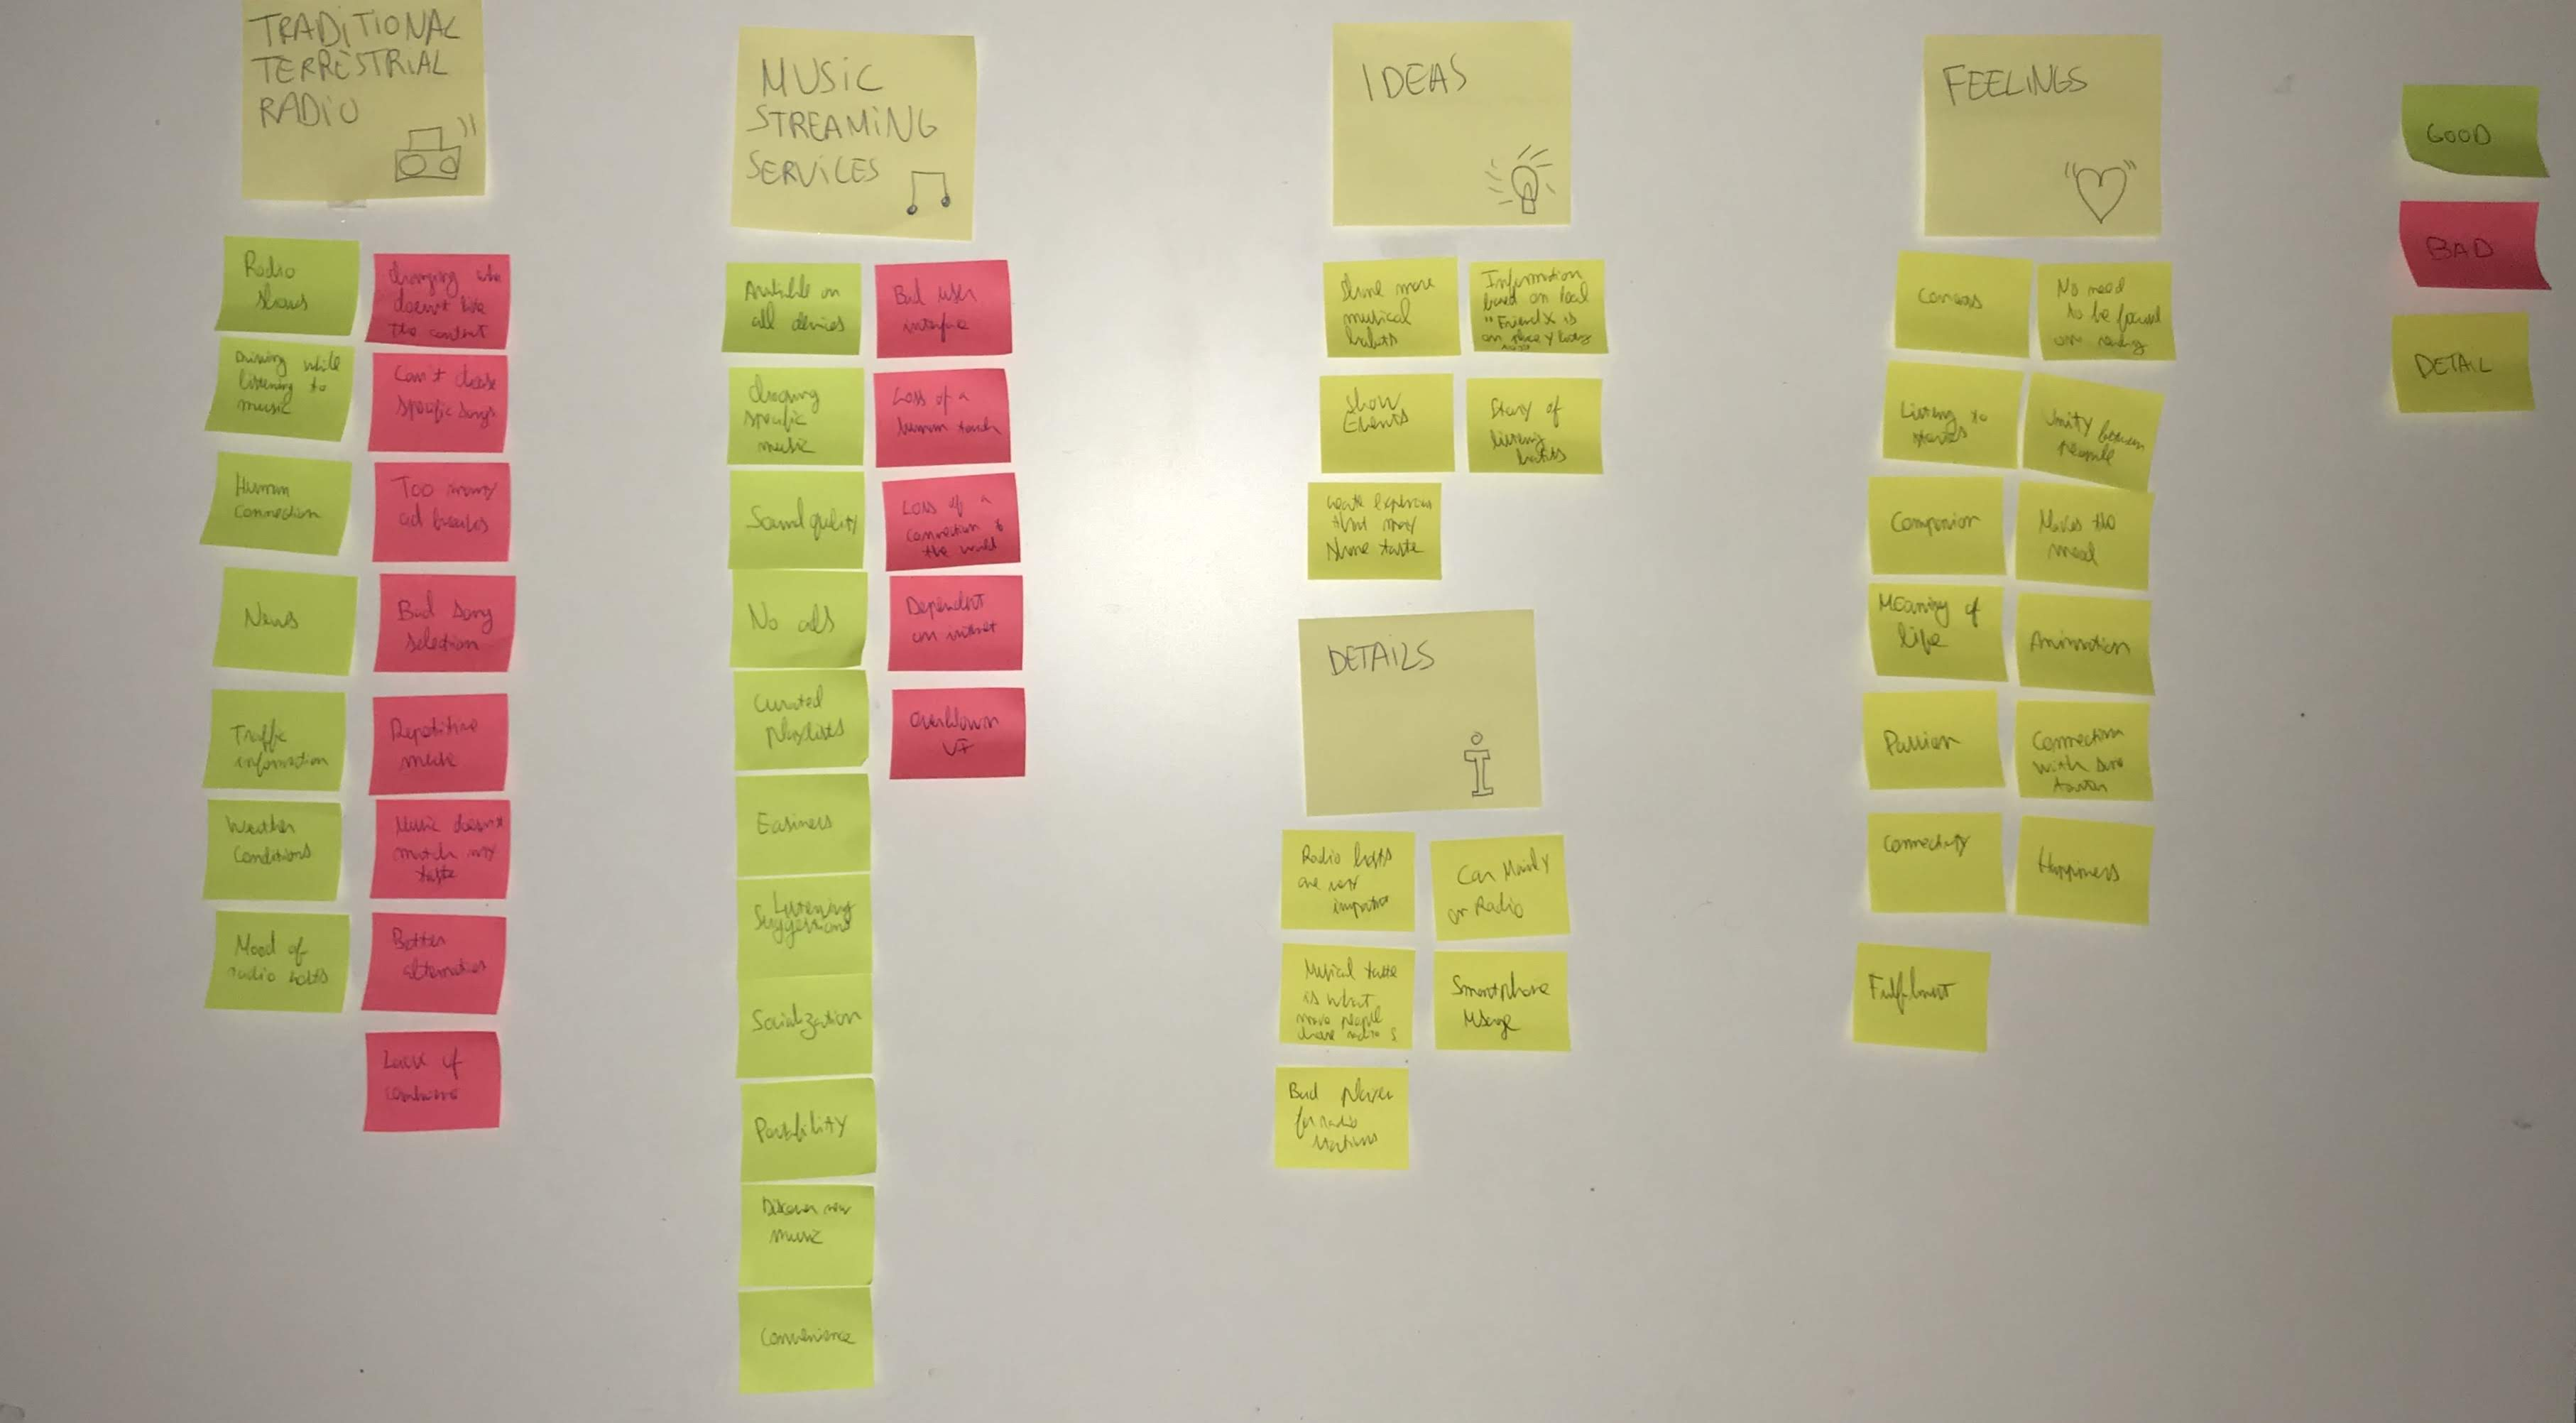
\includegraphics[width=0.8\textwidth]{./Images/finalaffinitydiagram.jpg}
\caption{Final affinity diagram with the gathered data from the diary study and interviews}
\label{fig:diagram2}
\end{figure}

The interviewees have given us important and detailed information regarding their audio consuming habits — how and why they listen to music and other audio content, which factors they value the most and the least in a listening session, and even some ideas and suggestions to implement and take into account when designing our solution. For instance, they noted that the social aspects of music streaming services and terrestrial radio are one of the most important aspects in their listening experience. The expressed empathy will be taken into account when developing the final solution, as all the interviewees expressed that music plays an extremely important role in their routines, and the way they experience it is a pivotal attribute.

To help us explore a diverse group of early-stage concepts, and to reflect on their stature, we will use the \textit{speed dating} methodology, as proposed by Davidoff et al. ~\cite{Davidoff2007}. Speed dating supports low-cost rapid comparison of design opportunities and situated applications by creating structured, bounded, serial engagements, based on the user research we delineated in this section. In return, by structuring a comparison of concepts, this method will assist us on the contextualization of multiple applications, as well as of critical aspects of individual applications, helping us in the identification and understanding of contextual risk factors, and how we can develop approaches to address them. Section ~\ref{sec:speeddating} will describe the developed work in the ambit of this concept.
% If Printing on DOUBLE SIDED pages, the second page should be white.
% Otherwise, comment the following command:
\cleardoublepage
%
%Chapter 4
% #############################################################################
% This is Chapter 4
% !TEX root = ../main.tex
% #############################################################################
% Change the Name of the Chapter i the following line
\fancychapter{Speed Dating}
\cleardoublepage
% The following line allows to ref this chapter
\label{chap:implement}

Speed Dating is a design method for rapidly exploring application concepts, their interactions, and contextual dimensions, requiring no technology implementation. It was developed at Carnegie Mellon University for accessing finer-grained insights into user needs, and identifying critical contextual dimensions for the design space ~\cite{Davidoff2007}. The main drive for developing such methodology was the lack of availability of methods that help design teams transition from ideation to iteration. Moreover, the authors state that, in ubiquitous computing, important design and contextual risk factors are not discovered before the deployment of a system, which can have a significant negative impact on the course or viability of a given project.

Aiming at solving these issues, speed dating supports low-cost rapid comparison of design opportunities and situated applications by creating structured, bounded, serial engagements. In addition, it helps teams contextualize multiple implementations, as well as critical aspects of individual applications, quickly foregrounding potential precarious issues before any implementation. It tests the researcher's initial ideas of problem definition and scope against user needs and the contextual factors that underlie them, while minimizing costs and time demands. Speed dating enables the researcher to explore the outermost frontiers of the design space, "presenting users with scenarios that push social boundaries to uncover where these boundaries actually lie” ~\cite{Davidoff2007}.

This method consists of a two-stage process, settling between sketching and prototyping. The first stage, named 'need validation', involves the use of personas, scenarios, and storyboards in a process aimed at exposing and validating user needs. The second stage, labeled 'user enactments', combines experience prototyping strategies and key concepts from the speed dating method within the elicitation of a second round of feedback pointed at finding a more full run of conceivable outcomes for the design.

We chose to apply the speed dating methodology since it allowed us to get a deeper understanding of our users' needs, while at the same time increasing our design effectiveness and efficiency. This approach was essential in exploring the complex set of factors, contextual dimensions, and design considerations that characterize a diverse and ambitious project such as this one. In the following subsections, we describe the work we have conducted in each of the stages of this methodology.

\section{Need validation}

The need validation stage of speed dating consists of presenting a set of storyboards to a group of target users, to synchronize the design opportunities researchers found with the needs users perceive. These storyboards help designers prioritize user demands, map areas for innovation more clearly, and use that focus to narrow the design space for implied implementations. ~\cite{Davidoff2007}

The first step of this phase is to focus concepts on user needs, where teams generate and cluster concepts around the needs identified in the conducted research. ~\cite{Davidoff2007} This is achieved by creating a collection of personas and scenarios that fall on both sides of boundaries the design team has speculated on. 

\begin{figure}[!h]
    \centering
    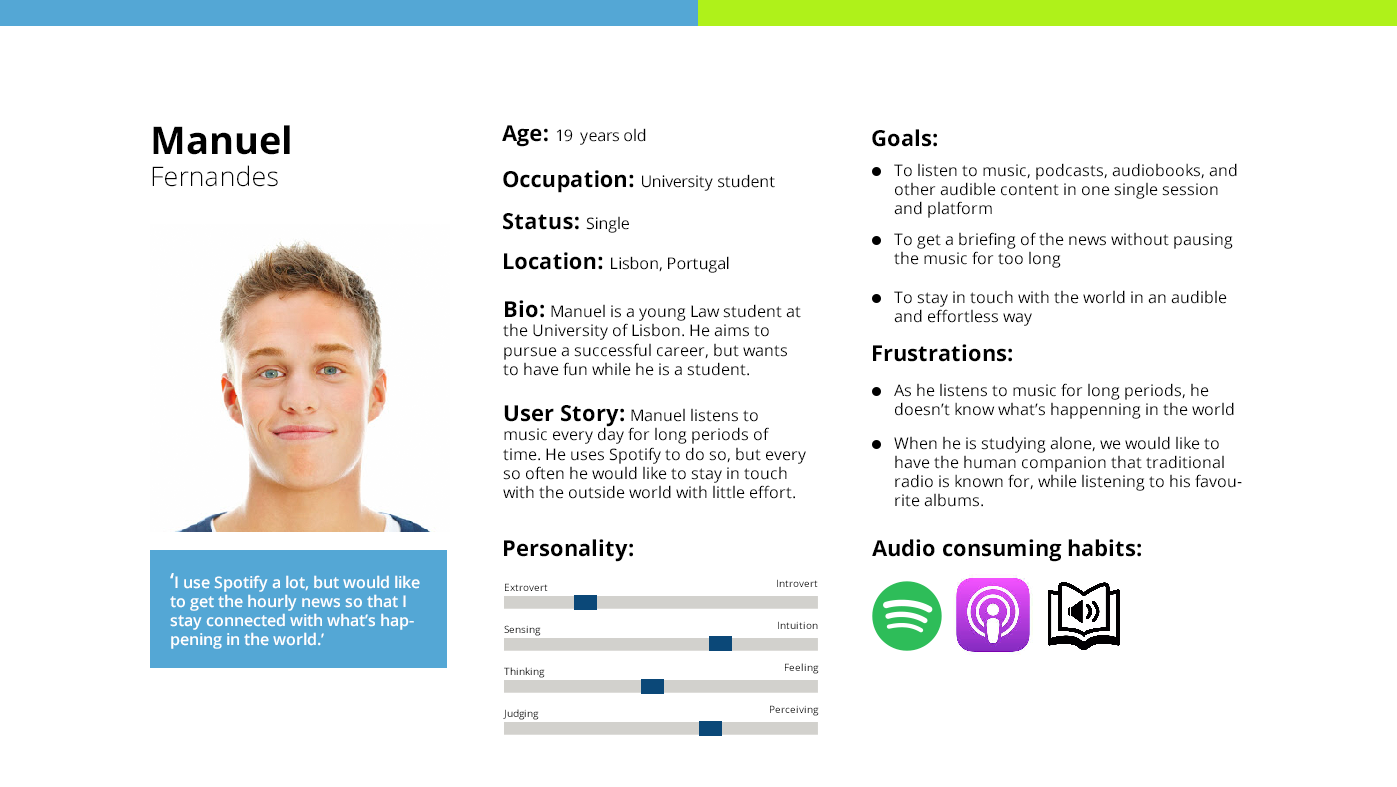
\includegraphics[width=\columnwidth]{./Images/persona.png}
    \caption{Example of one of the created personas.}
    \label{fig:persona}
\end{figure}

To do so, we have produced a set of four personas, based on four different potential users of this solution. To make them feel as real as possible, each persona was attributed an age, occupation, status, location, biography, user story, goals, frustrations, personality traits, and audio media consuming habits. The latter attribute is the main characteristic that differentiates the created personas from each other, so that we can understand if the portrayed functionalities of this platform would appeal to all ranges of potential users, even those that don't have very substantial audio listening habits on their routines. A summary of each persona is presented in the following list:

\begin{itemize}
	\item Manuel Fernandes, a university student that is a power-user of Spotify, who feels 'disconnected' from the world while indulging in all-day music listening sessions using the on-demand service;
	\item Carolina Santos, a software engineer that enjoys the interactivity of traditional terrestrial radio stations, but also enjoys the on-demand selection of her favorite songs that a music streaming service provides;
	\item Rita Silva, a middle-aged school teacher whose audio listening habits consist of a few minutes per day, tuning into her favorite radio station to listen to the news;
	\item Tomás Ventura, a truck driver that relies heavily on radio stations for his entertainment, but is getting tired of the repetitive music choice.
\end{itemize}


A subsequent set of scenarios was attributed to each of these four personas. Each scenario represents a distinct use case of this platform, focusing on situations where it is easy for participants to imagine themselves performing the mentioned activities.

We have represented these personas and their respective scenarios in a set of storyboards that document how each need arises in daily life, and how the concept intervenes to improve the quality of life. To develop such materials, we have begun by using the traditional sketching method by drawing these storyboards on paper.

\begin{figure}[!h]
    \centering
    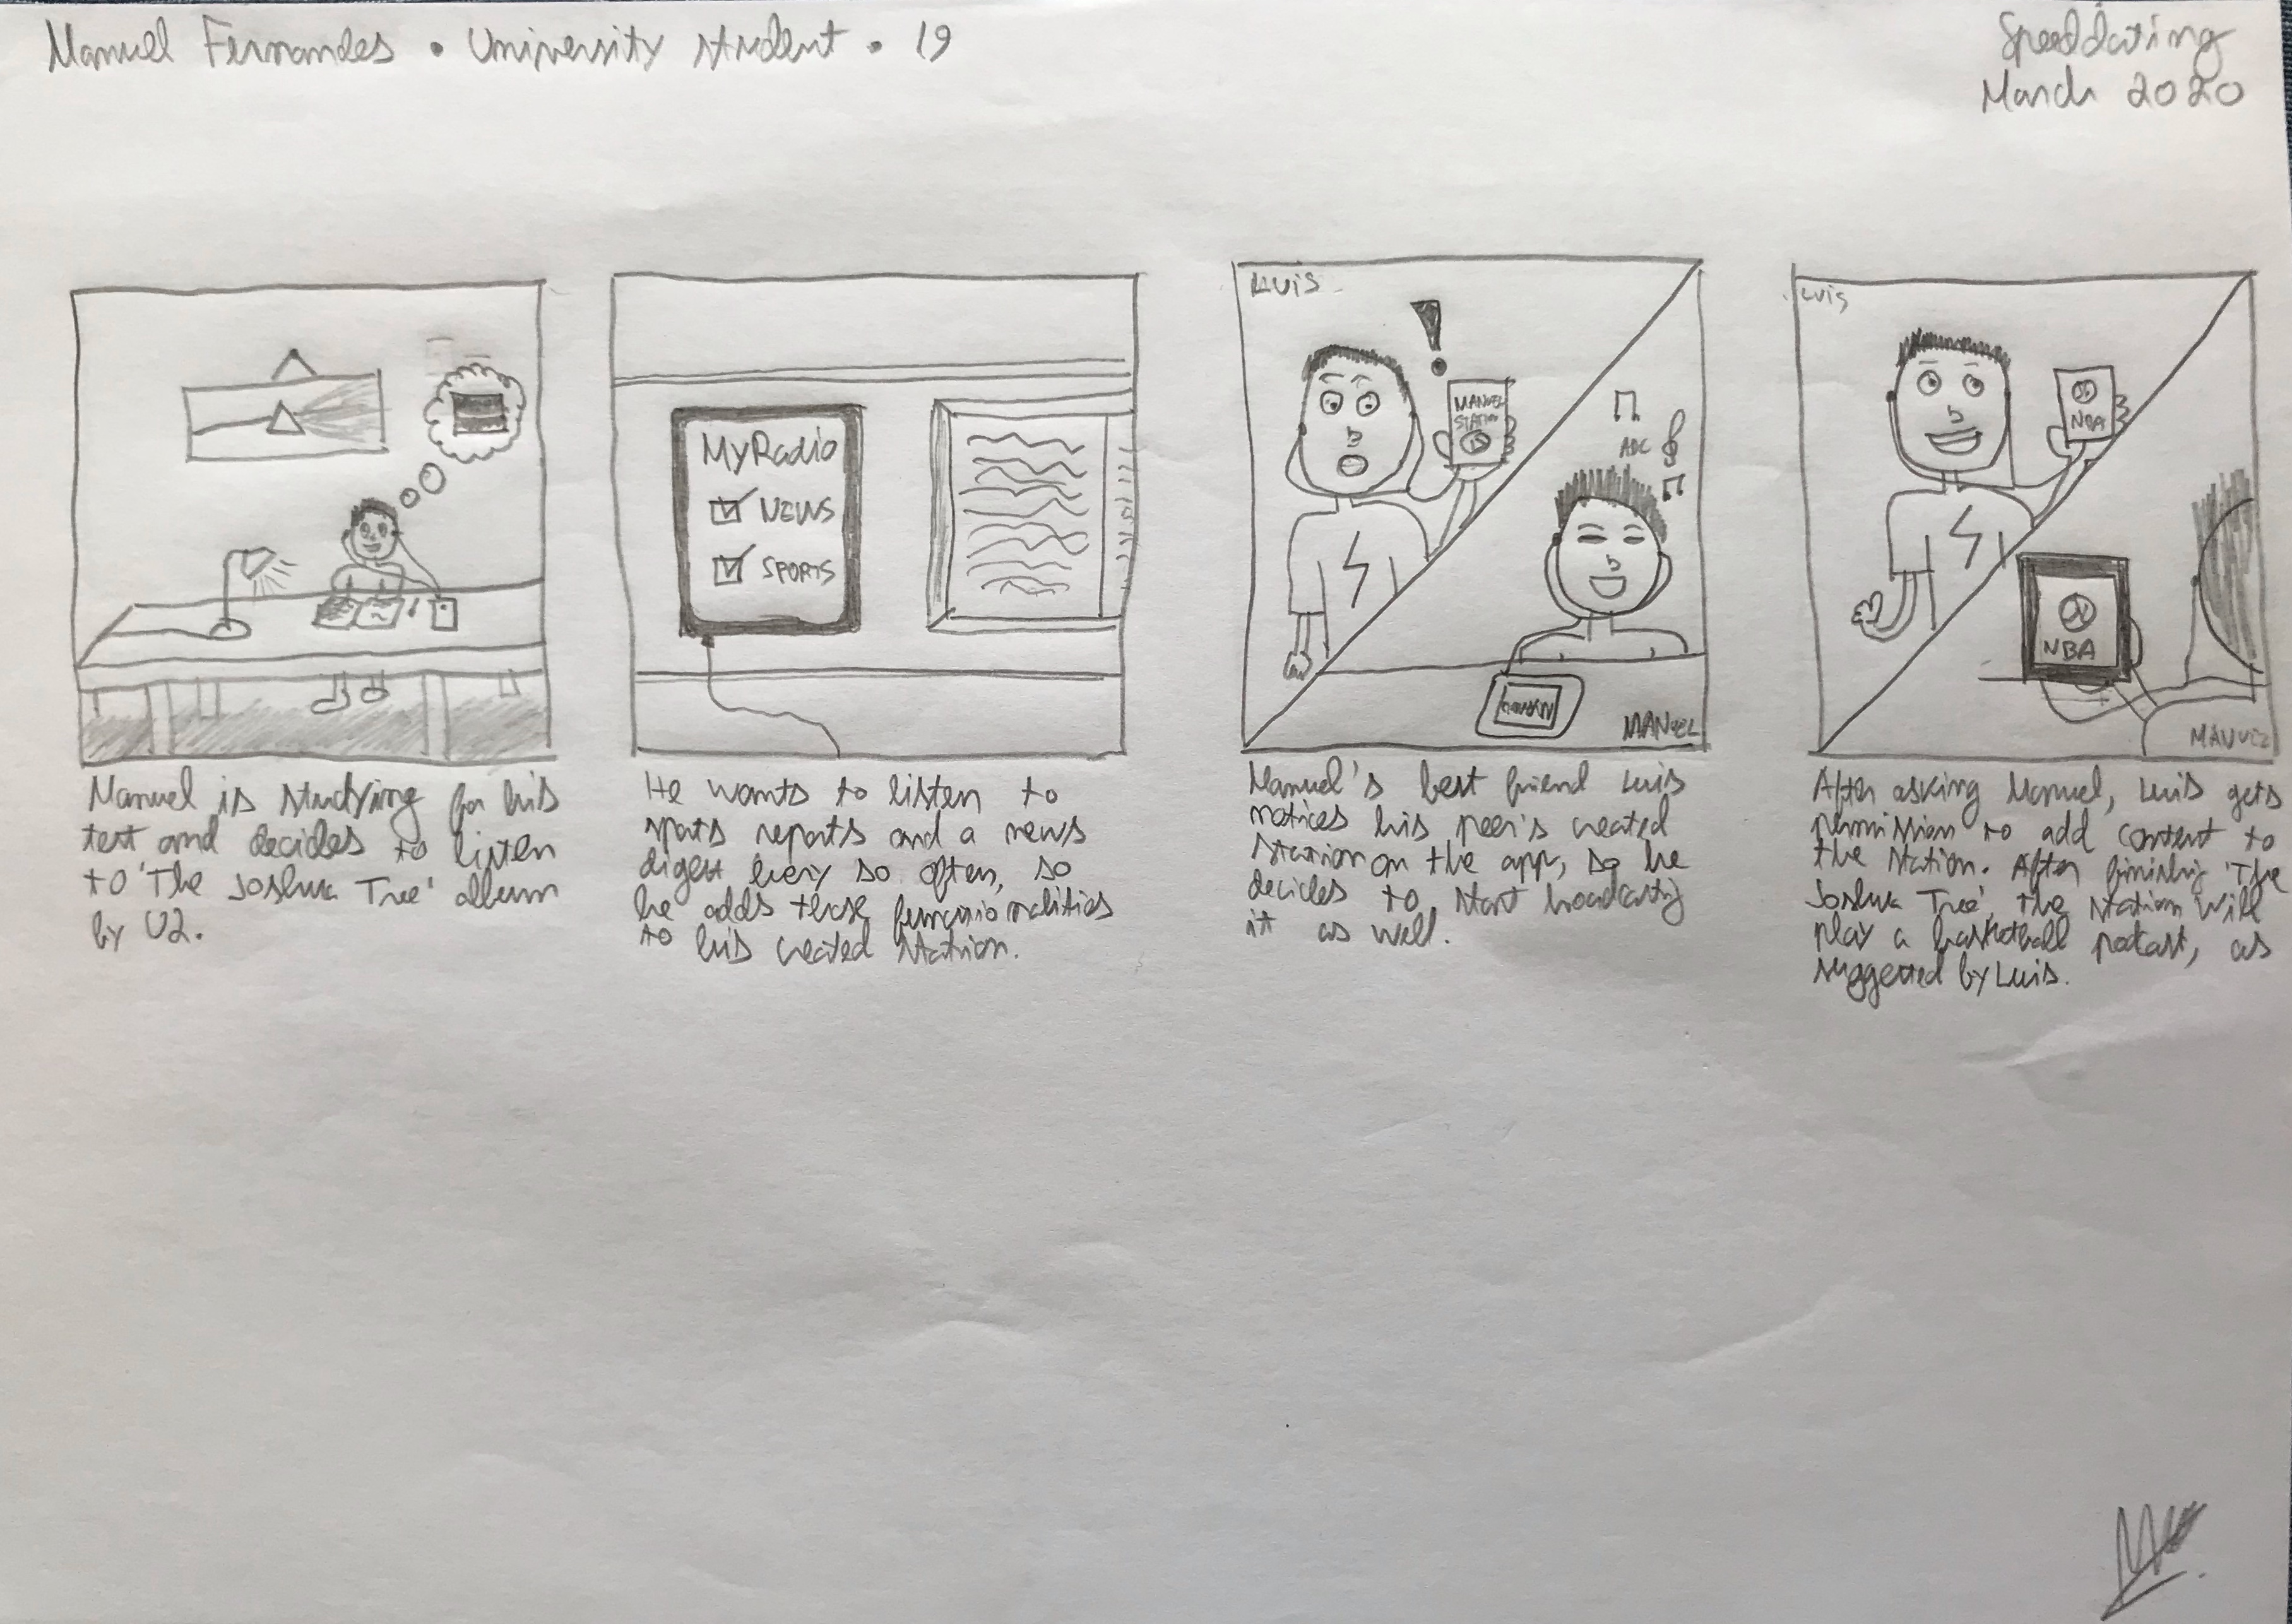
\includegraphics[width=\columnwidth]{./Images/storyboard.jpg}
    \caption{Example of one of the created storyboards, with the 'Manuel Fernandes' persona.}
    \label{fig:storyboard}
\end{figure}

The next step was to conduct a session where we presented this set of storyboards to small groups of target users. The original guidelines of the speed dating methodology state that these sessions should happen in a physical location; yet, as our study was conducted amid the 2020 COVID-19 pandemic, we had to circumvent this challenge, to comply with social distancing measures imposed by our country. Thus, we have conducted a total of five remote sessions, via the Google Meet platform: three of them with users ranging from 18 to 24 years old; one with ages ranging from 25 to 35 years old; and a final session with ages ranging from 35 to 55 years old. The participating users are reported in table ~\ref{tab:users}. The duration of each session ranged from 30 to 45 minutes. The audio of the session was recorded with the consent of all participating users, in order to facilitate the note-taking and analyzing processes. A consent form was digitally signed by all participating users.


\begin{table}[]
\begin{tabular}{|c|c|c|c|c|}
\hline
\multirow{2}{*}{\textbf{Age}} & \multicolumn{2}{c|}{\textbf{Preliminary User Research}} & \multicolumn{2}{c|}{\textbf{Speed Dating}}          \\ \cline{2-5} 
                              & \textbf{Diary Study}        & \textbf{Interview}        & \textbf{Need Validation} & \textbf{User Enactments} \\ \hline
18 & \checkmark & \checkmark & \checkmark & \checkmark \\ \hline
18 &   &   & \checkmark & \checkmark \\ \hline
18 &   &   & \checkmark & \checkmark \\ \hline
19 &   &   &   & \checkmark \\ \hline
19 &   &   & \checkmark & \checkmark \\ \hline
20 &   &   & \checkmark & \checkmark \\ \hline
21 & \checkmark & \checkmark &   &   \\ \hline
22 & \checkmark & \checkmark & \checkmark & \checkmark \\ \hline
22 & \checkmark & \checkmark & \checkmark & \checkmark \\ \hline
22 & \checkmark & \checkmark &   &   \\ \hline
22 & \checkmark & \checkmark &   &   \\ \hline
22 & \checkmark & \checkmark &   &   \\ \hline
22 & \checkmark & \checkmark &   &   \\ \hline
22 &   &   & \checkmark & \checkmark \\ \hline
22 &   &   & \checkmark & \checkmark \\ \hline
22 &   &   & \checkmark & \checkmark \\ \hline
22 &   &   & \checkmark & \checkmark \\ \hline
22 &   &   &   & \checkmark \\ \hline
22 &   &   &   & \checkmark \\ \hline
24 &   &   & \checkmark & \checkmark \\ \hline
27 & \checkmark & \checkmark &   &   \\ \hline
32 &   &   &   & \checkmark \\ \hline
33 &   &   &   & \checkmark \\ \hline
36 &   &   & \checkmark & \checkmark \\ \hline
38 &   &   &   & \checkmark \\ \hline
43 &   &   & \checkmark & \checkmark \\ \hline
43 &   &   & \checkmark & \checkmark \\ \hline
46 &   &   &   & \checkmark \\ \hline
49 &   &   & \checkmark & \checkmark \\ \hline
50 & \checkmark & \checkmark & \checkmark & \checkmark \\ \hline
51 &   &   & \checkmark & \checkmark \\ \hline
55 & \checkmark & \checkmark & \checkmark & \checkmark \\ \hline
61 &   &   &   & \checkmark \\ \hline
62 &   &   &   & \checkmark \\ \hline
\end{tabular}
\caption{Participating users in the preliminary user research and speed dating methodology activities.}
\label{tab:users}
\vspace{-4mm}
\end{table}

The sessions started with a brief description of the project and the goals of the discussion. Then, the developed personas and storyboards were shown digitally by sharing the screen and providing the link to the folder containing the files. To facilitate the understanding of these materials, we have transmuted the hand drawings into a digital representation; nevertheless, we presented both and asked users to try to focus on the hand drawings.

After presenting a given storyboard, users were asked to put themselves in the shoes of the correlated persona, and, with that in mind, they were encouraged to express comments, opinions, and comparisons. The discussion of each scenario was facilitated by a researcher that had the main goal of steering the dialogue to elicit user needs. Storyboard discussions were lively and focused on participants' reactions to the scenarios. When appropriate, participants were asked: "Would you do something like that?" or "What would you do differently?" and were encouraged to elaborate on their responses. The researcher also regularly asked participants for their feedback in identifying positive and negative aspects, what would they find useful in their own lives, and what would they change. 

The received feedback was very positive. Most users identified themselves with the younger developed personas (Manuel Fernandes and Carolina Santos), stating that this 'interactive radio' approach would significantly enhance their audio listening experience in their daily routines. As they use on-demand music streaming services for long periods of time, their listening experience becomes dreary and not interactive, generating a sense of disconnection to the outside world. Yet, as they embraced these personas, users stated that this feeling would be practically nonexistent. Finally, the social and community features described in Manuel's storyboard were very well received, which proves the user demand for more social and community features to arise in modern audio consuming mediums. Conversely, users didn't see the advantage of incorporating more personal tidbits of information into personalized radio stations, such as location sharing or voice messages from their friends, as described in the older personas (Rita Silva and Tomás Ventura). Instead, users stated that they would prefer to have their social feeds to be delivered, rather than more personal, decontextualized, and sensible types of information.

After conducting the sessions, we extracted the most relevant statements that were recorded, which helped us reveal new design opportunities, while at the same time recognizing the ones that don't consist of a general user need or demand. We have discussed the users' reactions to concepts, prioritizing needs that emerge strongly in both user research and validation sessions. With the received feedback, we were able to reduce our design dimensions by three main extents, which will be further employed in the second phase of the speed dating methodology.

\section{User enactments}

The second and final phase of the speed dating methodology, labeled 'user enactments', consists of creating a matrix of critical design issues, triggering the writing of dramatic scenarios that address the permutations of these issues. Researchers then ask participants to enact a specific role they regularly play as they walk through the scenarios, within an inexpensive, low-fidelity simulation of the target environment. ~\cite{Davidoff2007}

As a result of the need validation process, we were able to reduce our design dimensions by three main dimensions: 'Create', 'Listen', and 'Share'. These represent the three primary types of interactions with the system. 'Create' refers to the creation of a personalized station, where the user selects their desired audible content, as well as the station's schedule and preferences. 'Listen' invokes the actual listening experience of these stations, whether created by a given user or otherwise, in the context of the users' daily routines. Finally, 'Share' addresses the shareability and the community features of the system, such as simultaneous listening or station sharing.

We further identified an additional set of time-based dimensions through this process: 'Initiate', 'Employ', and 'Explore \& Customize'. 'Initiate' refers to a novel user interaction. 'Employ' refers to a response from the system, from which the user can interact with it. 'Explore \& Customize' refers to the users' probing and engagement of the available personalization features on the platform, from within a certain interaction or otherwise.

Using the above described design dimensions, we generated a matrix for carrying out speed enactments, shown in table ~\ref{tab:sdmatrix}. The first set of dimensions ('Create', 'Listen', and 'Share') align along the vertical axis, while the second set ('Initiate', 'Employ', and 'Explore \& Customize') align along the horizontal axis. The cells contain fictional scenarios that capture the intersection of types of interactions with stages of a system event. In the interest of keeping participants engaged and avoiding redundancy, we chose not to fill all of the cells in the matrix. 


\begin{table}[]
\begin{tabularx}{\columnwidth}{|l|X|X|X|}
\hline
\multirow{3}{*}{Create} &
  Initiate &
  Employ &
  Explore \& Customize \\ \cline{2-4} 
 &
  You create a radio station with a Spotify playlist, news about COVID-19, and weather information in Beja. &
  \multirow{2}{2.3cm}{The radio station is created and added to your stations’ library. A virtual radio host is assigned to your station. The schedule for your station is created automatically.} &
  \multirow{2}{2.3cm}{You further add radio blocks, such as a Twitter feed, and change the virtual radio host to a female Portuguese voice. You also tailor the schedule to your taste.} \\ \cline{2-2}
 &
  You create a radio station that is more news-focused, based on a library of pre-created stations that are suggested to you. &
   &
   \\ \hline
\multirow{2}{*}{Listen} &
  You start listening to the ‘Morning Station’ from your station library. &
  \multirow{2}{2.3cm}{The radio station is played with its specified settings.} &
  While listening, you choose to skip to a certain point of the station’s schedule. You also add a ‘Sports’ news block, as suggested by the player. \\ \cline{2-2} \cline{4-4} 
 &
  Before you start driving, you switch the ‘car’ mode and start playing to your ‘Driving’ station. &
   &
   \\ \hline
\multirow{3}{*}{Share} &
  You check the station your friend is listening to, and you decide to start listening to it as well. &
  You start listening to the same radio station, at the same point the participating users were listening. &
  You suggest the addition of a sports podcast radio block, to which your friend (the station creator) gives you permission to add. \\ \cline{2-4} 
 &
  You share one of your created stations with a small group of your friends, giving them the ability to edit the contents of the station. &
  Your friends can now start listening to your station. &
  A friend of yours adds a custom radio block, which enunciates the voice messages from their WhatsApp group. \\ \cline{2-4} 
 &
  You choose to share one of your created stations with the whole platform’s community, being publicly available to anyone. &
  Your station is now available to all users, ready to be played, and it has 226 followers now. &
   \\ \hline
\end{tabularx}
\caption{Speed matrix generated for user enactments.}
\label{tab:sdmatrix}
\vspace{-4mm}
\end{table}


Based on the presented table, we have developed a medium fidelity prototype aimed at showcasing a preliminary concept of the Sterio platform to the common user. The prototype focused on merging a users' music streaming service library and audio dynamically generated from news, social networks, or even personal sources, with non-speech audio sound effects and background music. In this first stage, we focused on the 'create' and 'listen' design dimensions, which resulted in the creation of a set of dummy and non-technical screens to avoid possible distractions concerning superficial design considerations.

Users were guided through this set of dummy screens that enabled them to create and listen to a personalized radio station. This dummy station included a playlist from Spotify, breaking news about the COVID-19 topic, and weather information based on a dummy location. When reaching the final screen of the prototype, an audio file that contained the 'selected' items was played. To keep users focused, the audio had a small duration of two and half minutes. The audio file also included snippets of two songs (from the 'selected' playlist) and radio-like transitions and sound effects, so that the station would feel as natural as possible to the user. Users were encouraged to try the prototype either on their desktop computers or on their smartphones, as the platform on which the prototype was built allowed both mediums.

\begin{figure}[!h]
    \centering
    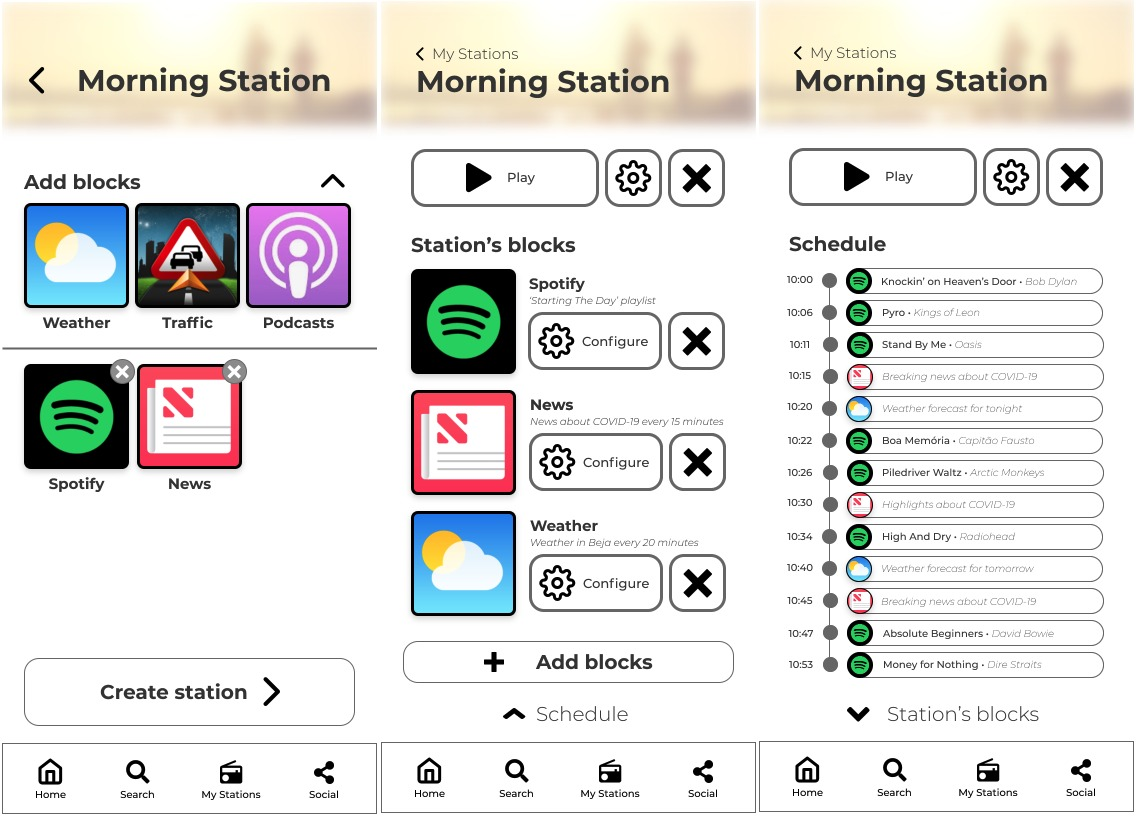
\includegraphics[width=\columnwidth]{./Images/prototype.jpg}
    \caption{Screenshots of the developed Sterio medium fidelity prototype.}
    \label{fig:persona}
\end{figure}

Given the before-mentioned COVID-19 pandemic we faced during the development of this study, the diffusion of the prototype was conducted using the WhatsApp social network, complying with social distancing restrictions. Groups with 4 users were created (larger numbers were avoided in order to make the discussion easier). In total, 7 groups of 4 people were created, totaling 28 participants in this study. 15 users were of ages ranging from 18 to 25, whilst the remaining 13 were of ages ranging from 26 to 62. The participating users are reported in table ~\ref{tab:users}.

Since the discussion of this prototype was conducted using an instant messaging service, users were encouraged to share their opinions and engage in discussion with each other, providing useful feedback that should be taken into account when developing the final product. From the 28 users, 19 have participated in the need validation activity of the speed dating method, thus an introduction to the general concept of the platform wasn't necessary. The remaining 9 users were introduced to the main abstract of the project and were asked to sign a virtual consent form. Users were informed that the displayed interface was created for demonstration purposes only, and that it didn't match the final product, shifting away their attention to the general concept of the system and not its usability.

The middle-fidelity prototype was created using three main tools: Adobe XD, Audacity, and macOS Text To Speech voices. 

Adobe XD was used for the development of the dummy interface. This platform allows playback of an audio file, which was convenient to showcase the final concept of the platform. The app also allows an easy sharing of the prototype, guiding them through its available options. 

Audacity was used to create the radio station audible file. The app allowed the editing of the audio file, making easy to expose how a created radio station would sound by gathered all the various audible elements (text-to-speech, music, and transitions). 

Finally, macOS' built-in text-to-speech software was used to synthesize into speech the content that the dummy user would provide (in this case, news and weather information). We opted for this solution since the operating system has a built-in European Portuguese voice (Catarina) that sounded very reliable and natural, making the development of the prototype a simpler task.

Corroborating with the first step of the method, the received feedback was very positive. All users clearly understood the main concept of the platform. Some of them mentioned that, in a first stage, they didn't understand the conceptualization on paper, but the prototype did enlighten them by showing in a visual and practical way how the platform would work.

Regarding the text-to-speech usage on the prototype, the feedback received was better than expected. The majority of users thought that the text-to-speech voice mimicking a radio host was more natural than what they were expecting. When asked if they felt a human element, and/or a connection with them in a similar way that traditional radio stations provide, all users replied affirmatively. In particular, older users accepted the text-to-speech functionalities quite well, with some mentioning that their original perception of this software (such as GPS turn-by-turn instructions) was out-blown with the use of this particular voice. Some younger users noted that the pronunciation of a small set of words was not clear or sounded unnatural, mainly new words (such as 'COVID-19') or foreignisms. Nevertheless, most of them noted that the advantages of using this technology outweigh the drawbacks.

Most users noted that they would use the platform on a daily basis, while others said it would be particularly interesting to use on specific occasions (such as driving or cooking). Some suggestions for future implementation on the system were also given by the users, such as the possibility for selecting their desired voice in their language, or a ‘quick station’ feature for the times when they would like to listen to a personalized radio based on their taste without a higher level of customization.
% If Printing on DOUBLE SIDED pages, the second page should be white.
% Otherwise, comment the following command:
\cleardoublepage
%
%Chapter 5
% #############################################################################
% This is Chapter 5
% !TEX root = ../main.tex
% #############################################################################
% Change the Name of the Chapter i the following line
\fancychapter{Sterio System}
\cleardoublepage
% The following line allows to ref this chapter
\label{chap:steriosystem}

To understand the tasks that our platform must fulfill, the first steps we have taken were an investigation and analysis of the currently available music streaming platforms and terrestrial radio stations, identifying the strengths, weaknesses, and opportunities of each. At the same time, we have conducted a study on the available literature that addresses these mediums and the vital concept of interactive radio. Further, we have overseen a thorough user research study by conducting a survey, a diary study, and interviews, and, most importantly, by applying the speed dating method. As we're applying user-centered design and human-computer interaction principles and methodologies, our users must be involved in the development of the project from the very early stages. This will maximize the quality of the user experience of the solution, and the earlier the user is involved, the less repair work needs to be done at the final stages of the project's life cycles.~\cite{Courage2005}

After the presented research, we can identify our opportunity and act upon it. As such, in the first stage, we need to determine our requirements and accordingly plan the features and tasks that are going to be made available on the platform to fulfill our users' desires. The gathered datasets from sections ~\ref{chap:relatedwork}, ~\ref{chap:userresearch}, and ~\ref{sec:speeddating} provided pivotal information that helped fulfill this task. Then, after we've outlined the goals that our platform must satisfy, we can outset the development of a functional prototype with a working feature set and near ready for general-purpose usage.

In this section, we explain in greater detail the development process that led us to the final \textit{Sterio} platform. We begin by outlining the requirements and goals that our solution must fulfill. Afterward, we discuss and examine the adopted technologies and services, as well as the overall architecture of the system. Finally, we present a complete overhaul of the crafted features by describing the methods, technical facets, and reasoning behind all components of the application.


% #############################################################################
\section{Requirements} 
\label{sec:req}

Taking into account all the conducted research regarding previous work, and by identifying and understanding our users' needs, we were able to identify a concrete set of features that we expect our solution to tackle. These features can be described as followed:

\begin{itemize}
	\item Creation of personalized radio stations, allowing users to select their desired audio content (by songs, albums, artists, playlists or others) using an on-demand music streaming service, or even add to the station other audio media content such as podcasts or audiobooks;
	\item A 'virtual radio host' based on text-to-speech technology is attributed to a given station, allowing content to be delivered in the periphery during that session (news, weather, traffic, social feeds, information about friends and family, and other types of readable information);
	\item A high level of customization of such radio stations and of its content must be available, allowing users to choose how often they would like to listen to each sort of content, the specific topics or themes of each audible content, the voice of the 'virtual radio-host' from the selection of the available text-to-speech voices, among other functionalities;
	\item The 'virtual radio host' mimics as best as possible a 'real' radio host, promoting interaction, human connection, and empathy between the listeners and their ‘own radio host’. Plus, audible divisors and elements, as well as other radio-familiar components are introduced along the session, so that these personal radio stations are as natural as possible, reassembling a 'real' radio station;
	\item A high level of shareability of the created radio stations, social/informative content, and other elements, allowing a simultaneous listening experience of radio stations among the platform's users, reproducing the same community feeling as traditional terrestrial radio, while at the same time indulging audio listeners in a social-network like atmosphere.
\end{itemize}

In the end, a general-purpose platform will emerge that creates a novel listening experience by merging the best functionalities of both music streaming services and traditional terrestrial radio in a personalized, integrated and social experience that may be shared with users' friends and family.


% #############################################################################


\section{Architecture}

The \textit{Sterio} platform was developed following a layered architecture, which not only supports the incremental development of systems, but also provides a changeable structure so that an equivalent layer can replace another one. Moreover, when a given layer is changed or updated, only its adjacent layer is affected. ~\cite{Aarsten} Every layer of the \textit{Sterio} system can be used individually with other similar applications or can be easily changed without compromising the other layers. 

The three main layers that compose our system are the Presentation, Business, and Database Layer, represented in Figure ~\ref{fig:arc}. In the following subsections, we explain in greater detail the role of each layer, as well as the reasoning and advantages of the used frameworks and technologies. 

\begin{figure}[h]
\centering
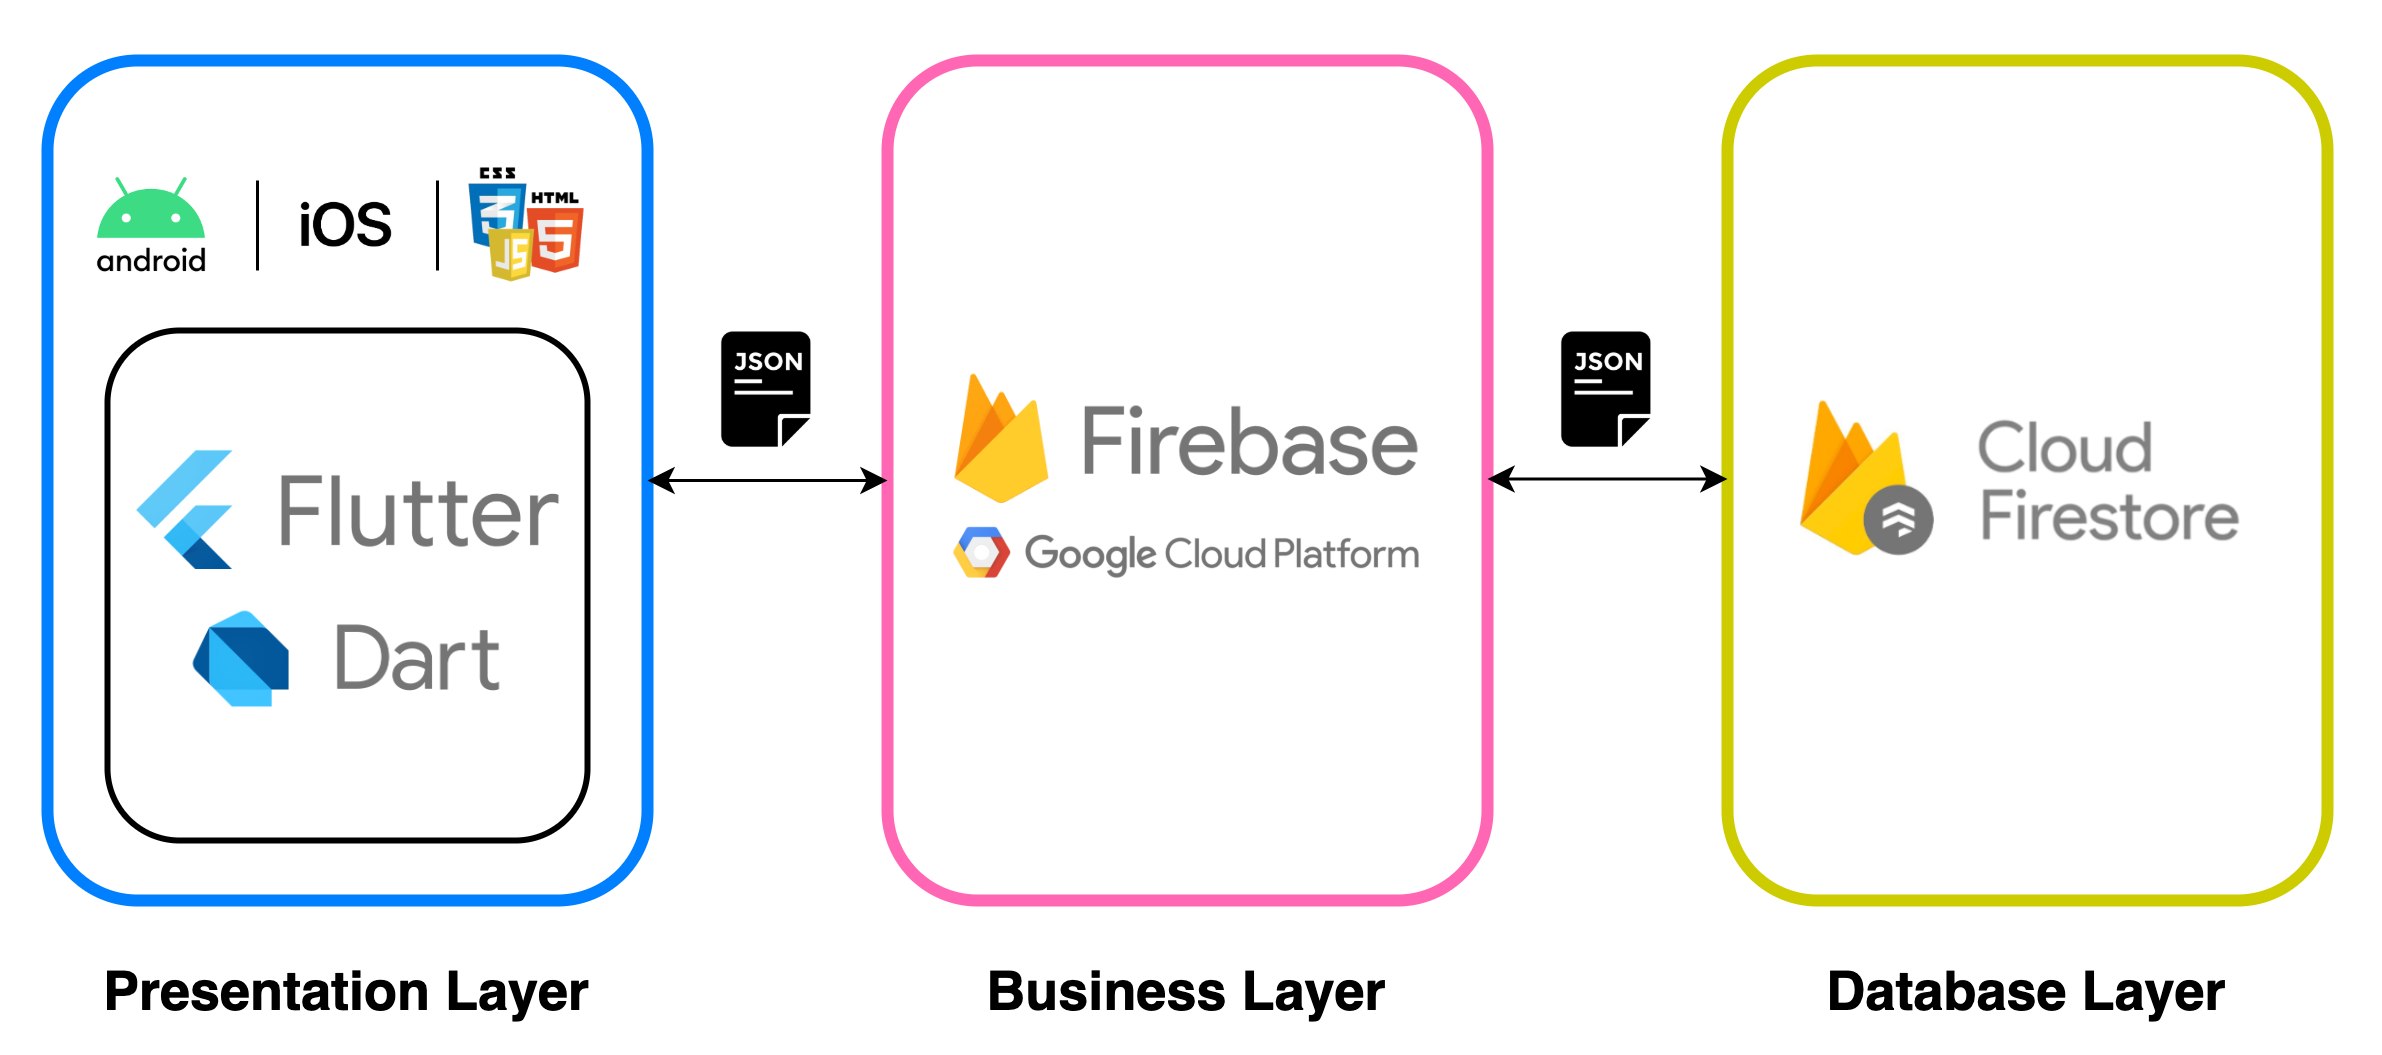
\includegraphics[width=0.8\textwidth]{./Images/arc.png}
\caption{Architecture of the Sterio system}
\label{fig:arc}
\end{figure}

\subsection{Database Layer}

The Database Layer is responsible for managing and storing all the data that it is used in the system. It receives information entered by the application's users and answers accordingly with the requested information from the Business Layer. ~\cite{Aarsten}

The first development step of the platform was the creation of an entity-relationship model so that we can model the database and determine which entities we need based on the medium-fidelity prototype described in section ~\ref{sec:userenactments}. The representation of this model, shown in Figure ~\ref{fig:eadiagram}, will help us visualize and conceptualize the system in the first stage, which will soothe the development difficulty and discard preliminary oversights.

\begin{figure}[h]
\centering
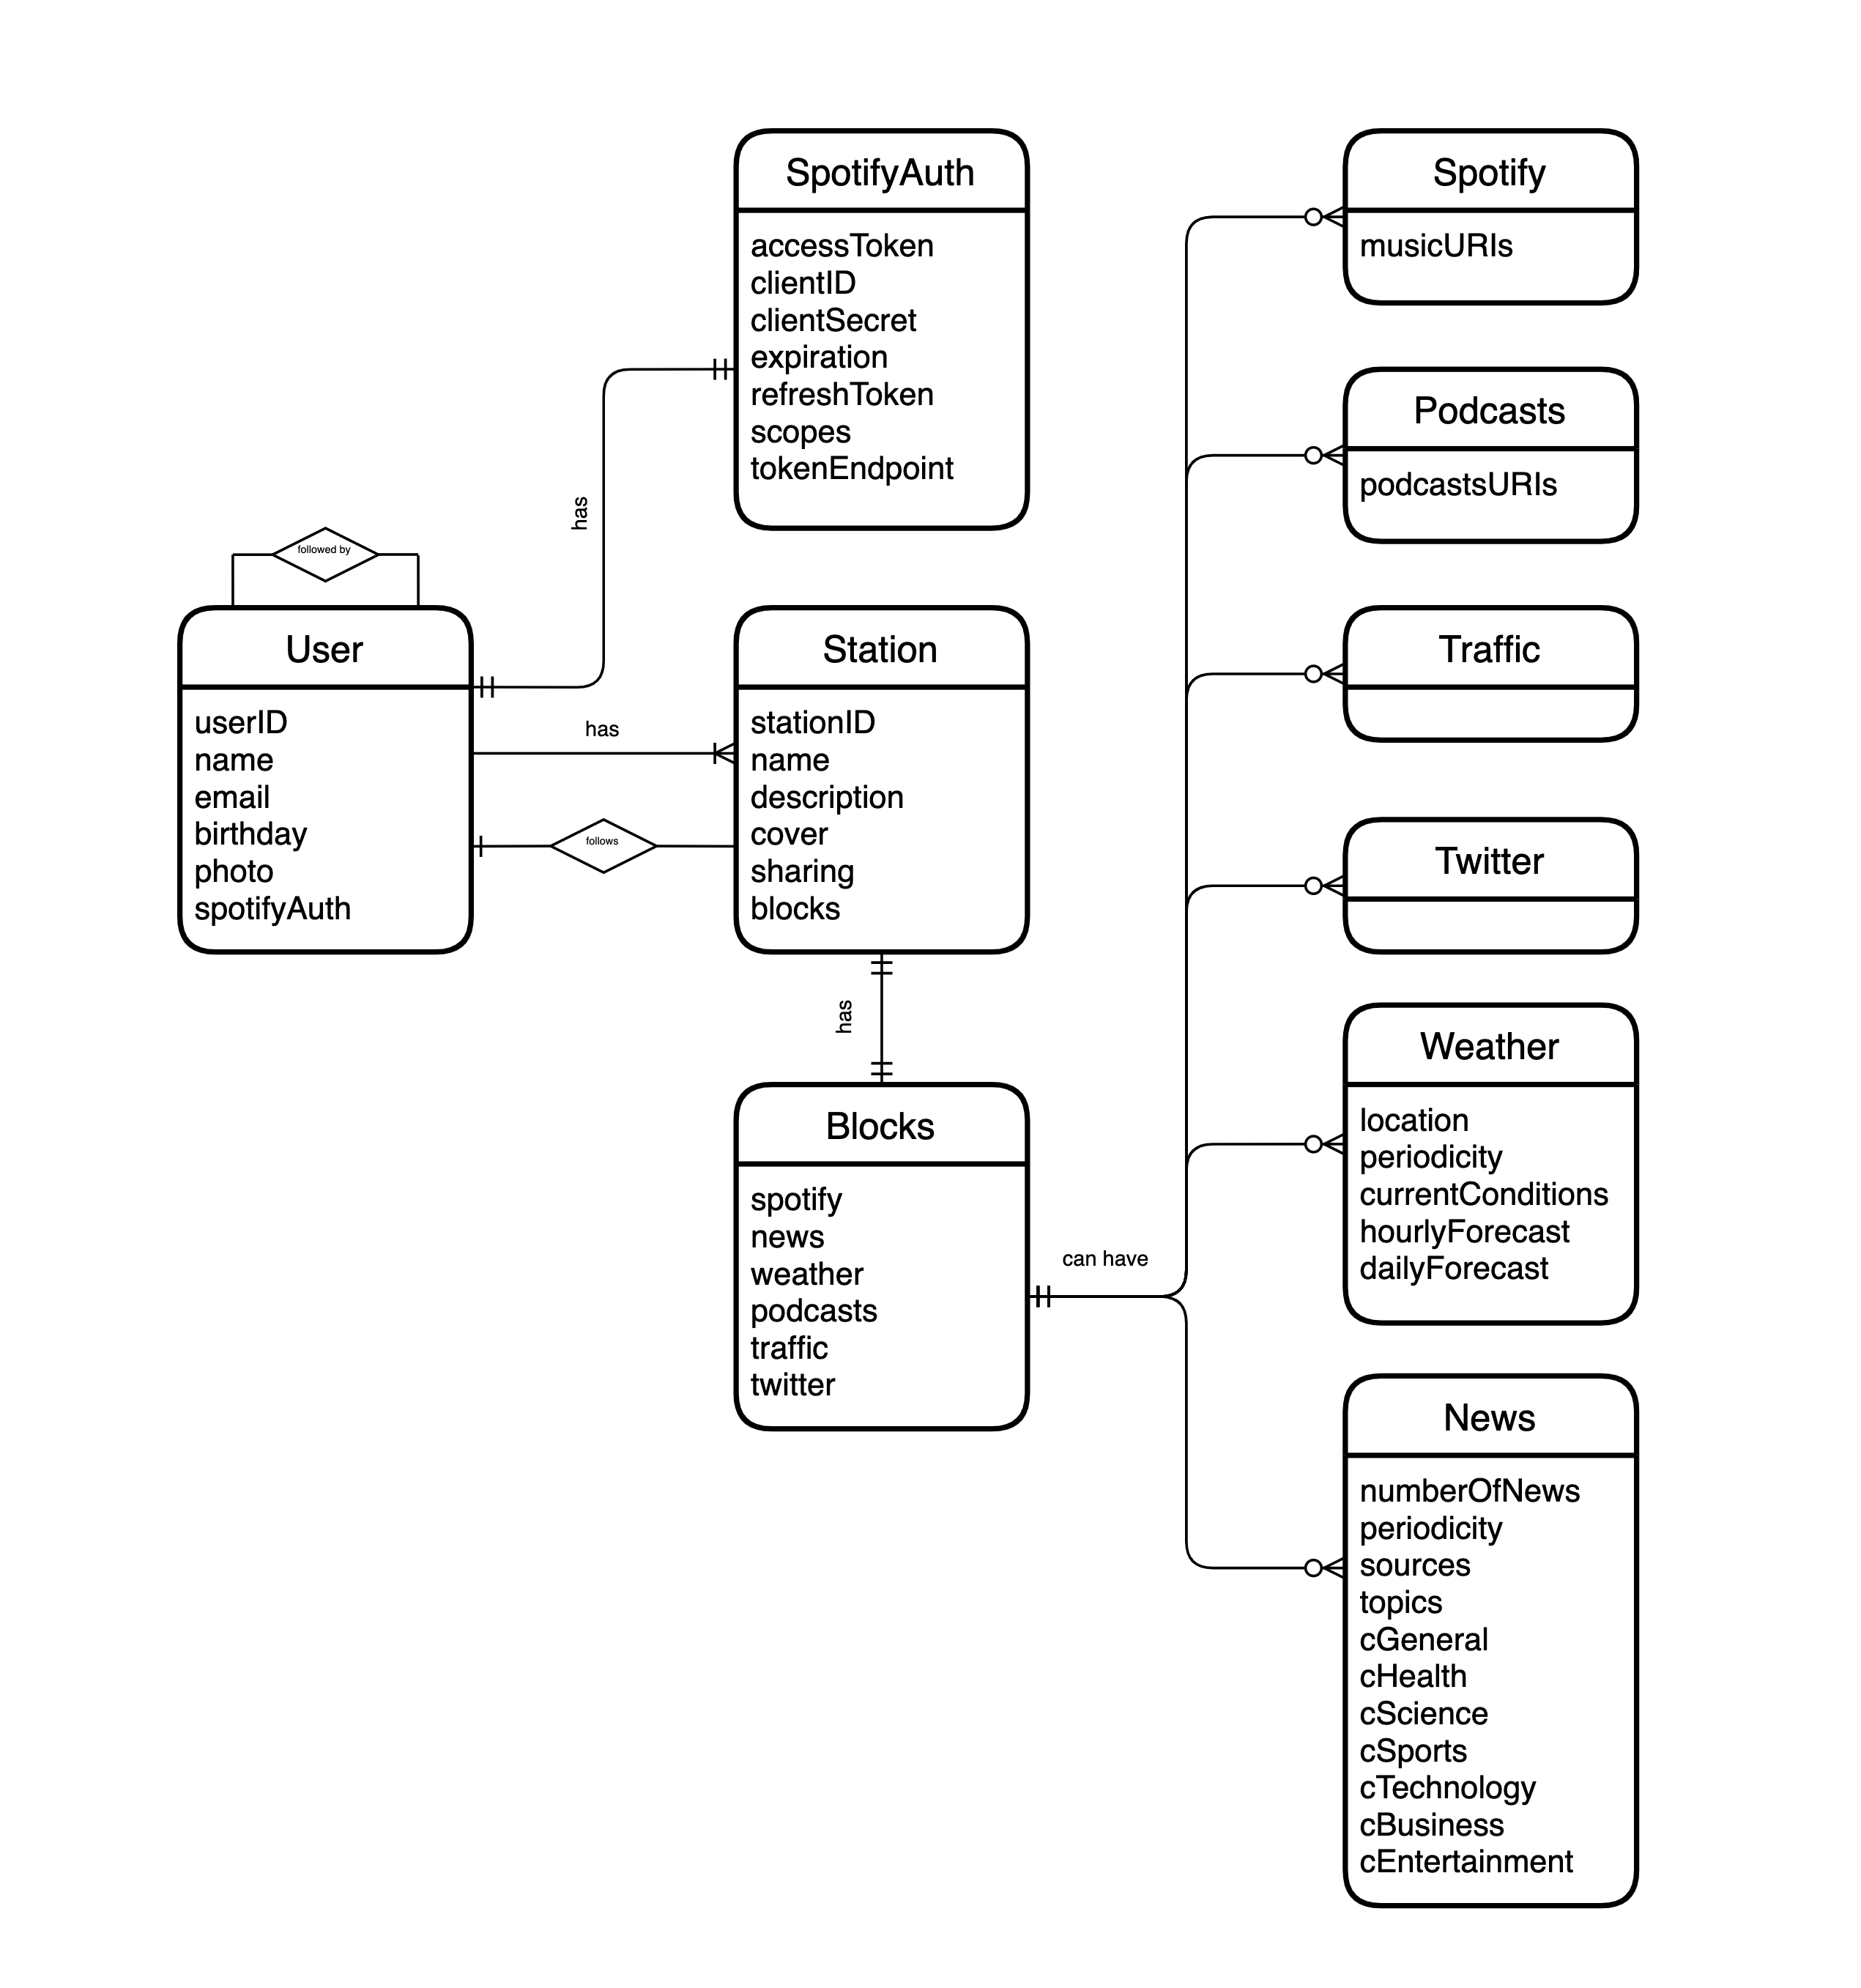
\includegraphics[width=0.8\textwidth]{./Images/ea.png}
\caption{Entity – Relationship Model of the Sterio system}
\label{fig:eadiagram}
\end{figure}


The implementation of the database was conducted using Google's Cloud Firestore~\footnote{Detailed information available on the platform's \href{https://firebase.google.com/products/firestore}{official website}.}, which is a NoSQL, document-oriented database. Being a NoSQL database, it provides several advantages, such as a non-relational and schema-less data model, low latency and high performance, highly scalable, and object-oriented programming that is easy and flexible to use. ~\cite{Stonebraker2010} Each document contains a set of key-value pairs, being optimized for storing sizable collections of small documents. It is a serverless document database that effortlessly scales to meet any demand, with no maintenance required, which accelerates the development of native cloud applications and lets developers focus their efforts on the most foreground layers of a system.

We chose to use Cloud Firestore due to its lean learning curve, ease-of-use, good performance, reliability, high scalability, and deep integration with other Google services that will also be used in the development of the platform. Furthermore, by using this technology, the system is prepared to be easily customized and to receive new data if the project has any changes in the way we approach some of its features.


\subsection{Business Layer}

The Business Layer is responsible for encoding the real-world business rules that determine how data can be created, stored, and changed. It contrasts with the remainder of the software that might be concerned with lower-level details of managing a database or displaying the user interface, system infrastructure, or generally connecting various parts of the program. ~\cite{Aarsten}

For the \textit{Sterio} platform, we chose to use Google's Firebase~\footnote{For more information on Google's Firebase and Cloud Platform services, visit its \href{https://firebase.google.com/}{official website}.} business logic features. Firebase is a \ac{MBaaS}, which is a model for providing web app and mobile app developers with a way to link their applications to backend cloud storage and \acp{API} exposed by backend applications while also providing features such as user management, push notifications, and integration with social networking services.

Firebase provides several pre-developed, robust, and reliable \acp{SDK} — such as authentication, hosting, storage, and app indexing — that helped us steer the focus of our development efforts to the design and conceiving of the user experience and interface. As with Cloud Firestore, it integrates thoroughly with other Google services — including the Google Cloud Platform, which will be used for the process and synthesizing of the text-to-speech technology — while also allowing the configuration of third-party \acp{API} that will be used in the context of our project.

\subsection{Presentation Layer}

The third and final layer of the system is the Presentation Layer, which is responsible for the interaction between the user and the system. ~\cite{Aarsten} This layer will interact with the business layer through calls to the Firebase service.

Based on the preliminary user research presented in Section ~\ref{chap:userresearch}, and corroborating with the data shown in Figure ~\ref{chart:devices}, most users listen to music streaming services on their smartphone. Furthermore, as we want our platform to be easily accessible on the go, we focused our efforts on analyzing the most popular mobile development frameworks to develop our platform on.

\begin{figure}
	\centering
	\caption{Share of internet users who have used a music streaming services in the last month worldwide in 2nd quarter 2017, by device (Statista / GlobalWebIndex)}
	\label{chart:devices}
	\begin{bchart}[step=10,max=45,unit=\%,width=0.8\textwidth]
        \bcbar[text=Smartphone (Mobile)]{39}
            \smallskip
        \bcbar[text=PC / Laptop]{30}
            \smallskip
        \bcbar[text=Tablet]{8}
    \end{bchart}
\end{figure}


We chose to develop the Sterio platform using Flutter~\footnote{To learn more about the Flutter framework, consult the \href{https://flutter.dev/}{official website}.}, which is an \ac{UI} toolkit for building natively compiled applications for mobile, web, and desktop from a single codebase. Flutter apps are written in the Dart~\footnote{For more information on the Dart programming language, visit its \href{https://dart.dev/}{official website}.} programming language and make use of many of the language's more advanced features. ~\cite{Payne2019}

In the context of our project, Flutter has some key advantages over other technologies. To start, although it has been built as a mobile-first toolkit in the first stage, Flutter is now a cross-platform development tool that allows the development of mobile (on the Android and iOS operating systems) and desktop apps without compounding changes to the codebase. This ensures that our platform renders well on a variety of devices and windows or screen sizes, without limiting our endeavors. ~\cite{H.GillbertMiller2011} Secondly, in comparison with other mobile frameworks, Flutter reduces the code development time by a wide margin. In a large and complex project such as ours, this is a crucial advantage that will lead us to a robust final product without the need for allocating umpteen resources. Finally, Flutter offers a variety of advanced tools that allow us to achieve a great user experience and interface design, which will help us achieve our goals. ~\cite{Payne2019}

% #############################################################################

\section{Functional Prototype}

Based on the medium-fidelity prototype presented in Section ~\ref{sec:userenactments}, the last — and most crucial — step of the development cycle was to construct a functional prototype with a fully-working set of features. This prototype should resemble as close as possible to the final representation of the system. 

In the following subsections, we describe in detail all functionalities, components, screens, implementations, and technical facets of the \textit{Sterio} system, as well as the design implications and limitations faced during the development of the prototype. We begin by examining the four main screens of the application — 'Home', 'Search', 'Social', and 'My Stations' — followed by an analysis of the technical reasoning behind our development rulings.

\newpage
\subsection{Login, Signup, and Authentication}
\label{subsec:lsa}

The first interaction the user has with the \textit{Sterio} platform is the login/signup screen, shown in Figure ~\ref{fig:login1}. There, the user can choose to login with an Apple or Facebook account, or with an e-mail. If the user chooses to use one of the first two methods, an in-app browser window is shown so that the user can enter the required credentials. If the user chooses to use an e-mail as a signup method, the screen is shown in ~\ref{fig:login2} is presented.

\begin{figure}[htbp]
	\centering
	\subfigure[Login / Signup screen]{\label{fig:login1}
	\frame{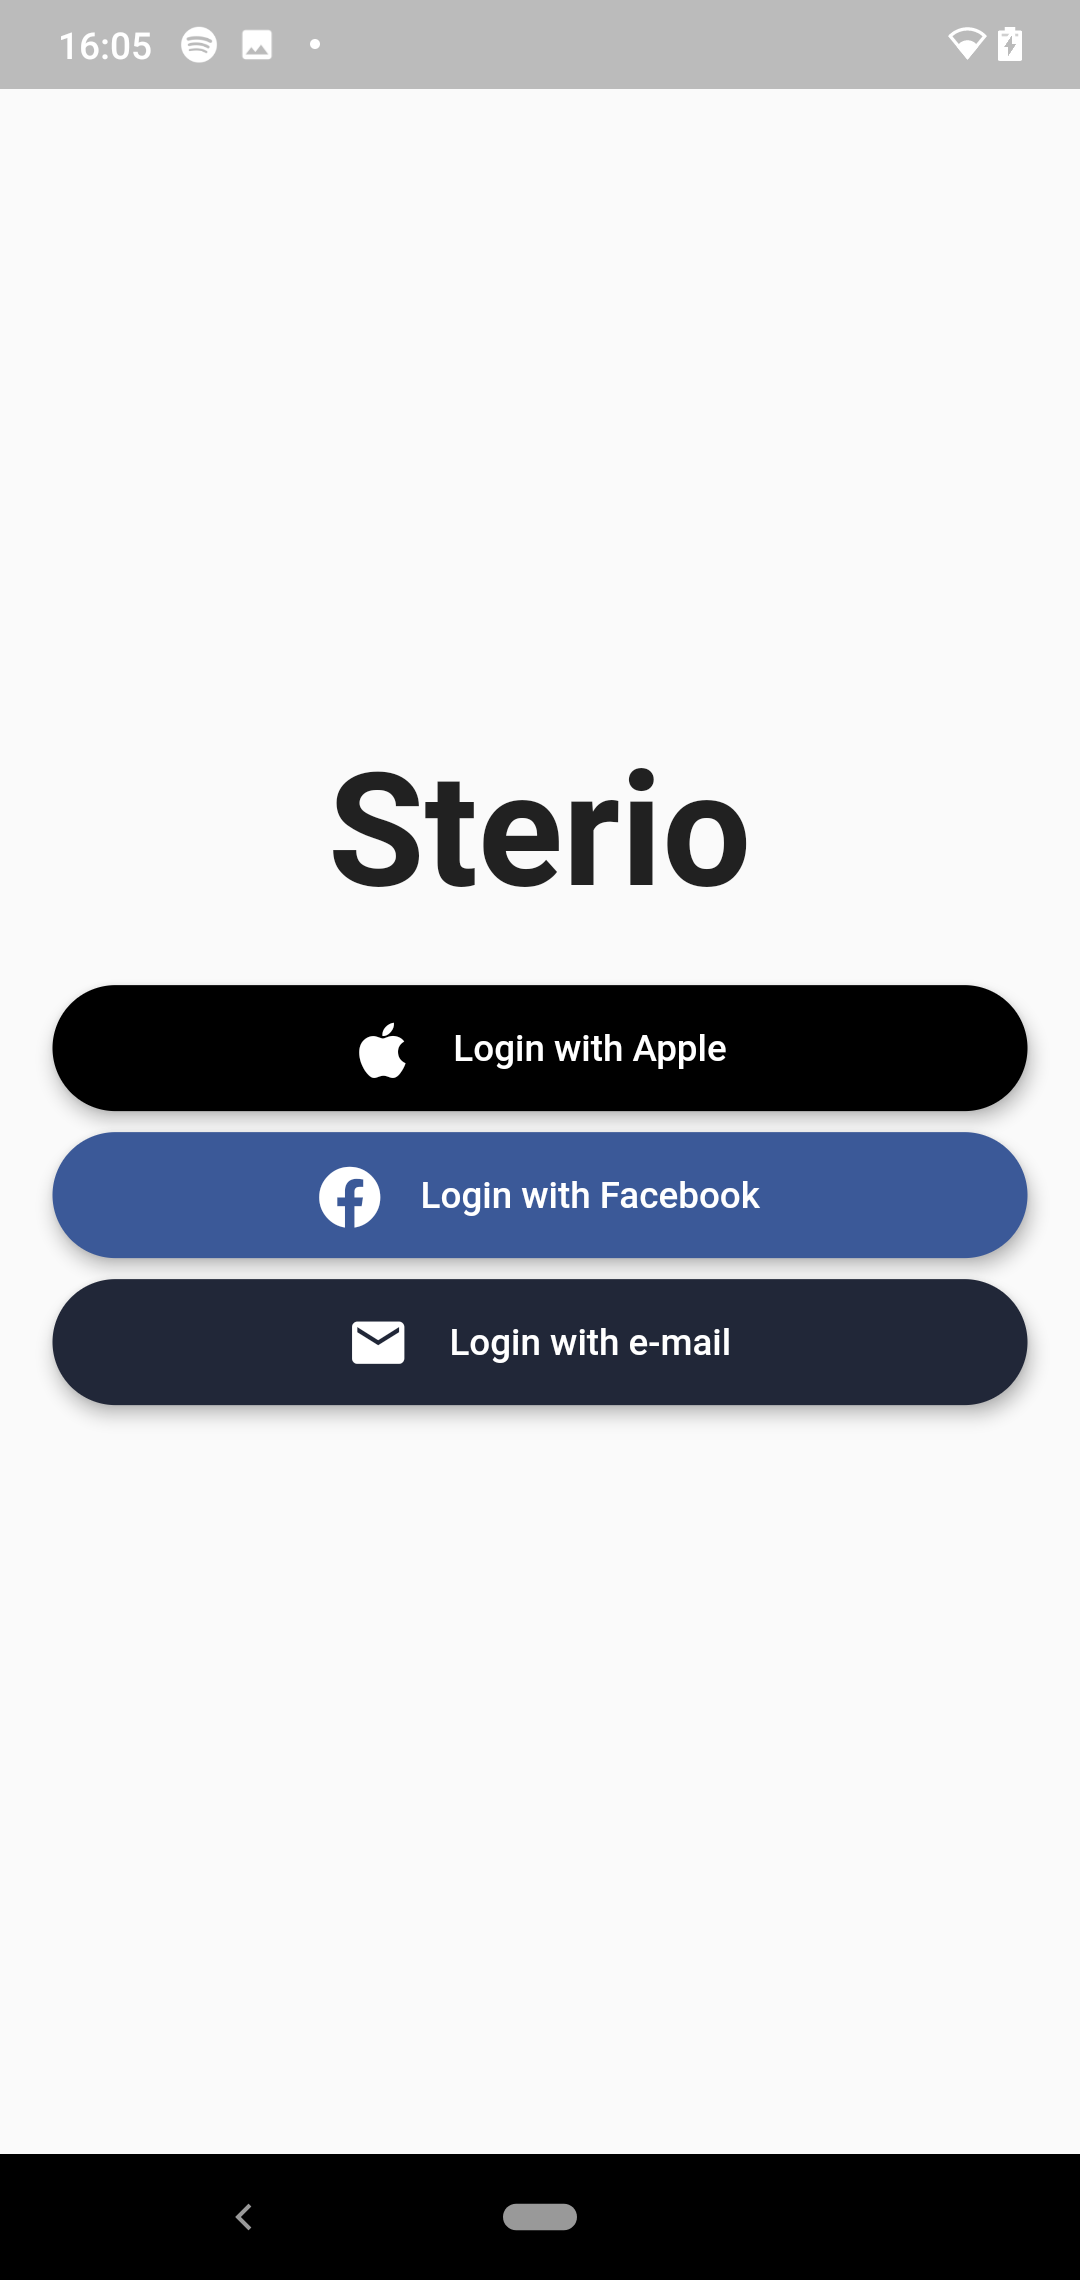
\includegraphics[width=0.29\textwidth]{./Images/screenshots/login1.png}}} \qquad
	\subfigure[Login with e-mail]{\label{fig:login2}
	\frame{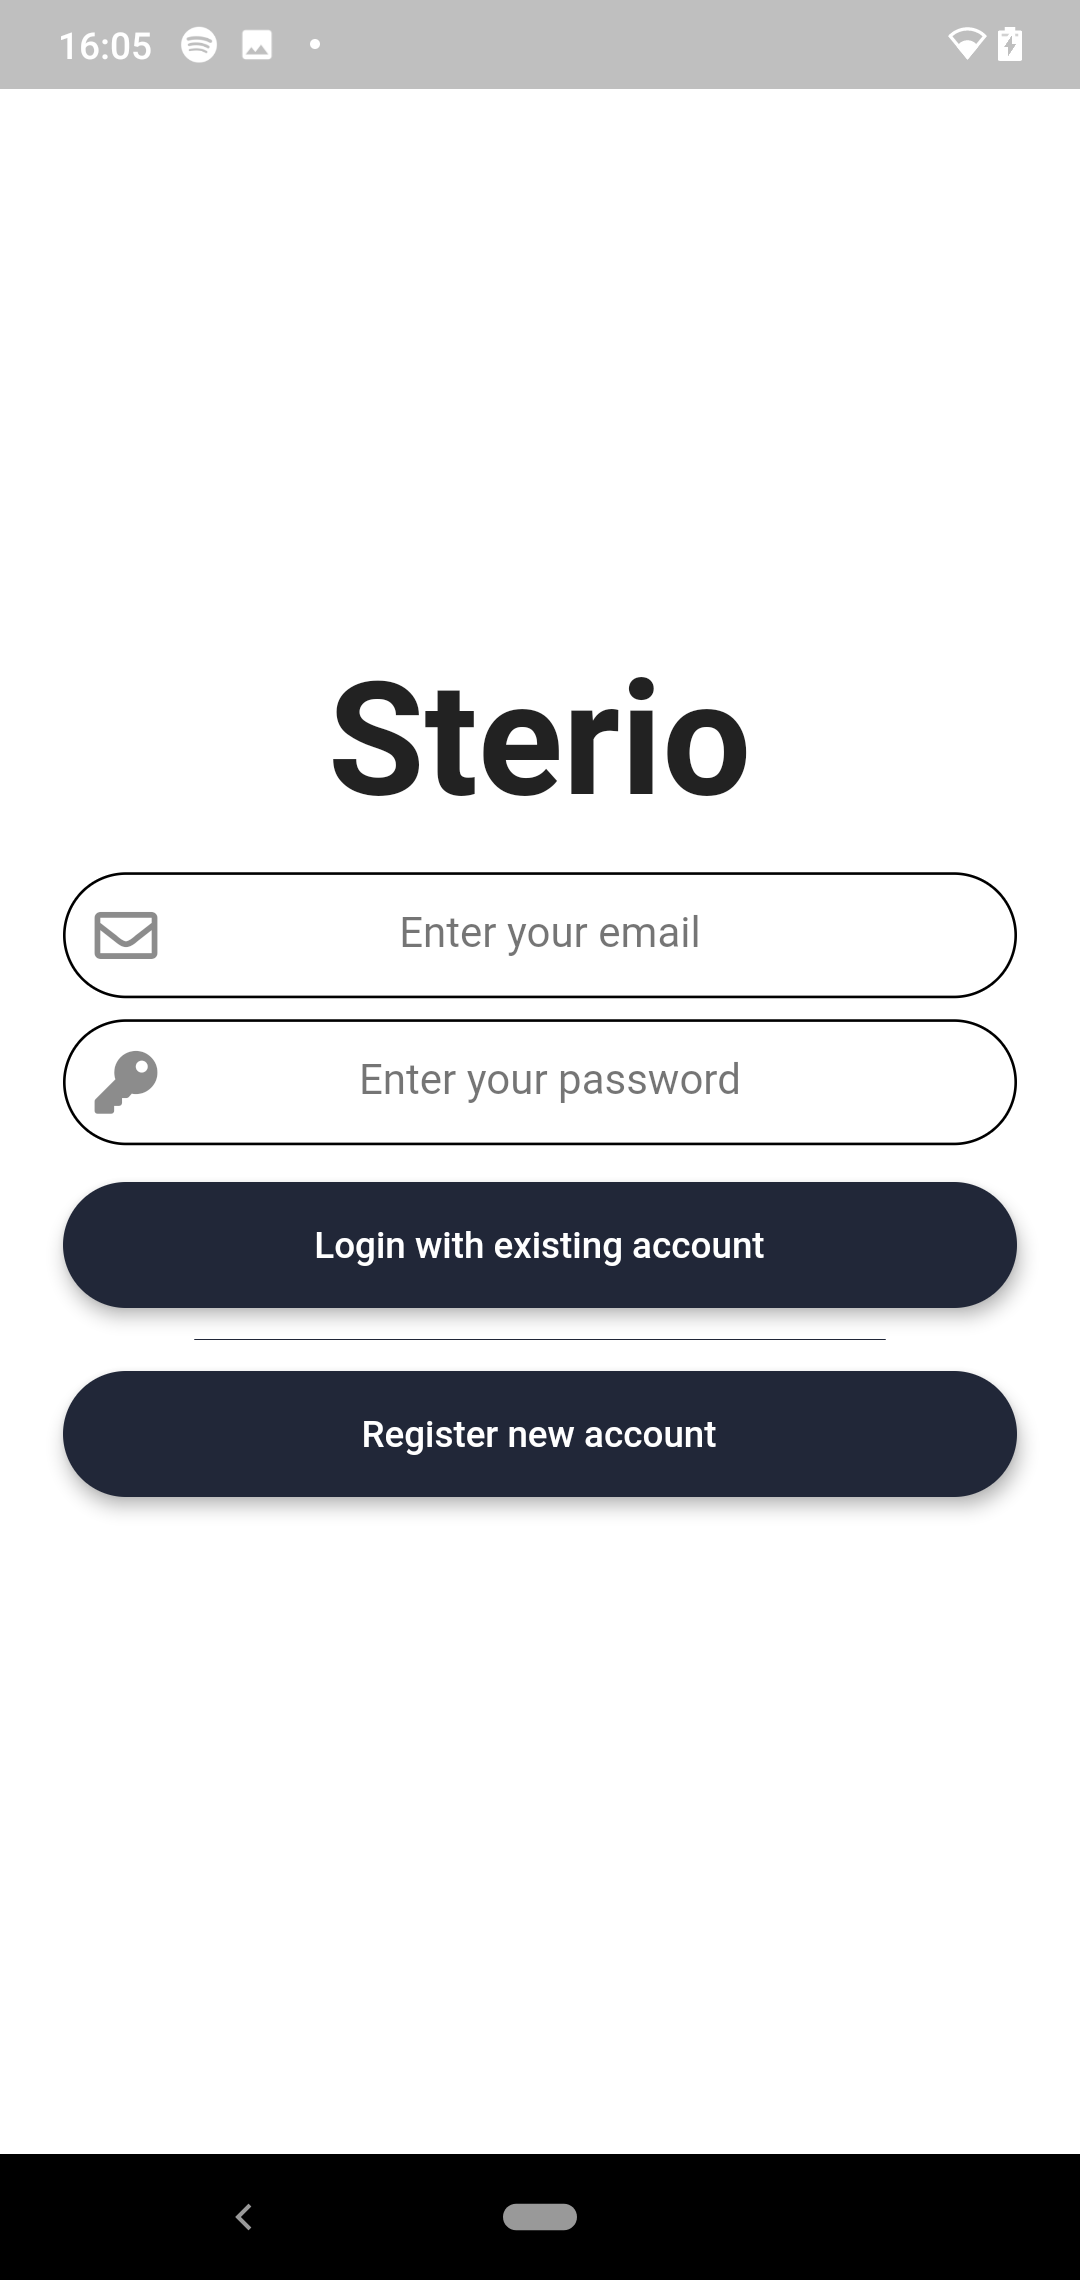
\includegraphics[width=0.29\textwidth]{./Images/screenshots/login2.png}}} \qquad
	\subfigure[Spotify authentication]{\label{fig:auth}
	\frame{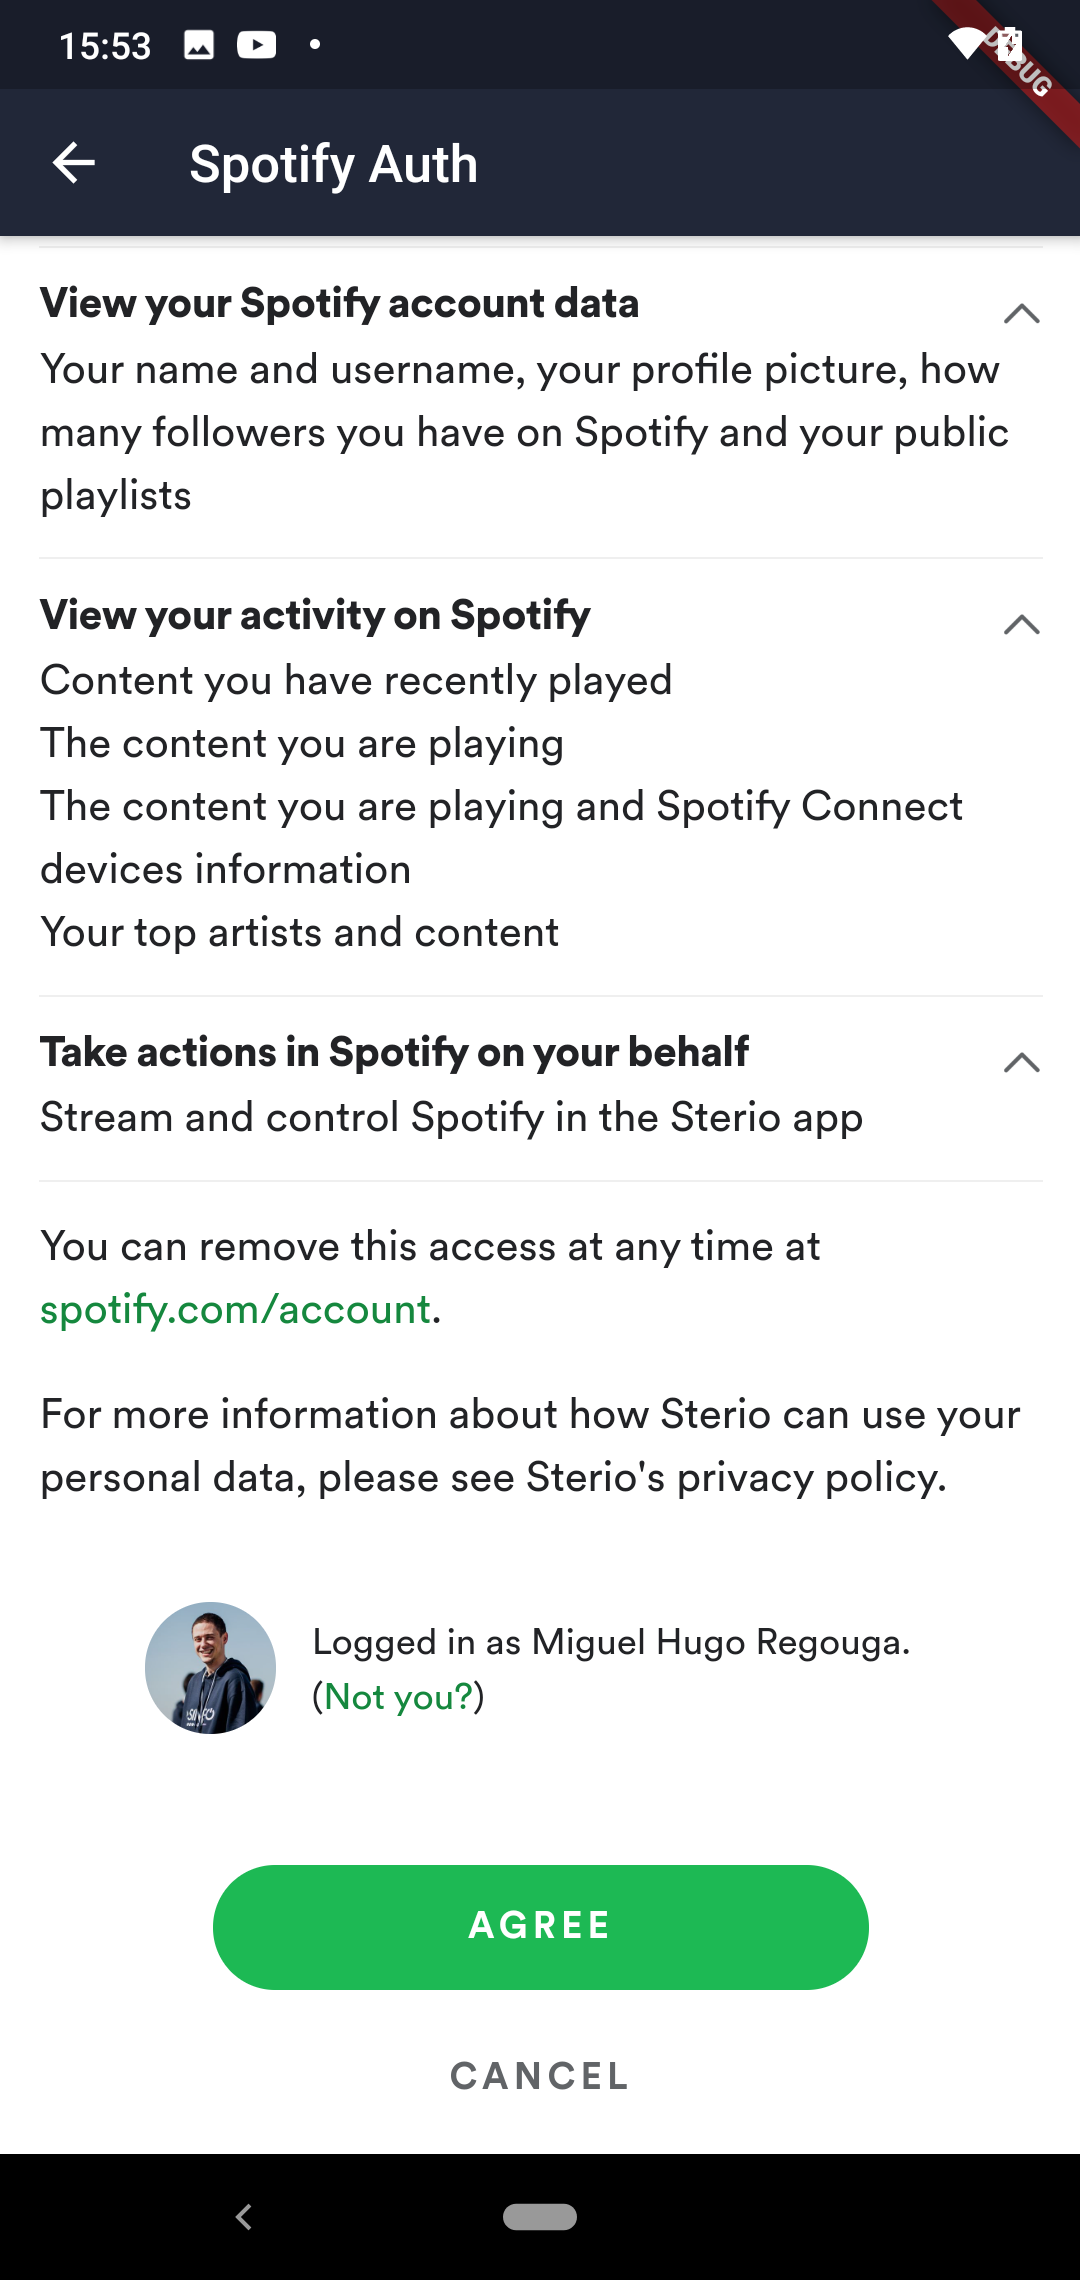
\includegraphics[width=0.29\textwidth]{./Images/screenshots/auth.png}}} \qquad
	\caption{Login, Signup, and Spotify authentication screens}
	\label{fig:lss}
\end{figure}

As the system integrates with a Spotify Premium account, it is also necessary that the user authenticates with the music streaming service, so that we can take advantage of its ~\ac{API}. To do so, an in-app browser window, shown in Figure ~\ref{fig:auth}, is also presented to the user. This is a one-time step, as the system stores the necessary ~\ac{API} parameters in the database and automatically logs in the user in future usages.

\newpage
\subsection{'Home' and 'Search' Screens}
\begin{figure}[htbp]
	\centering
	\subfigure['Home' screen]{\label{fig:homes}
	\frame{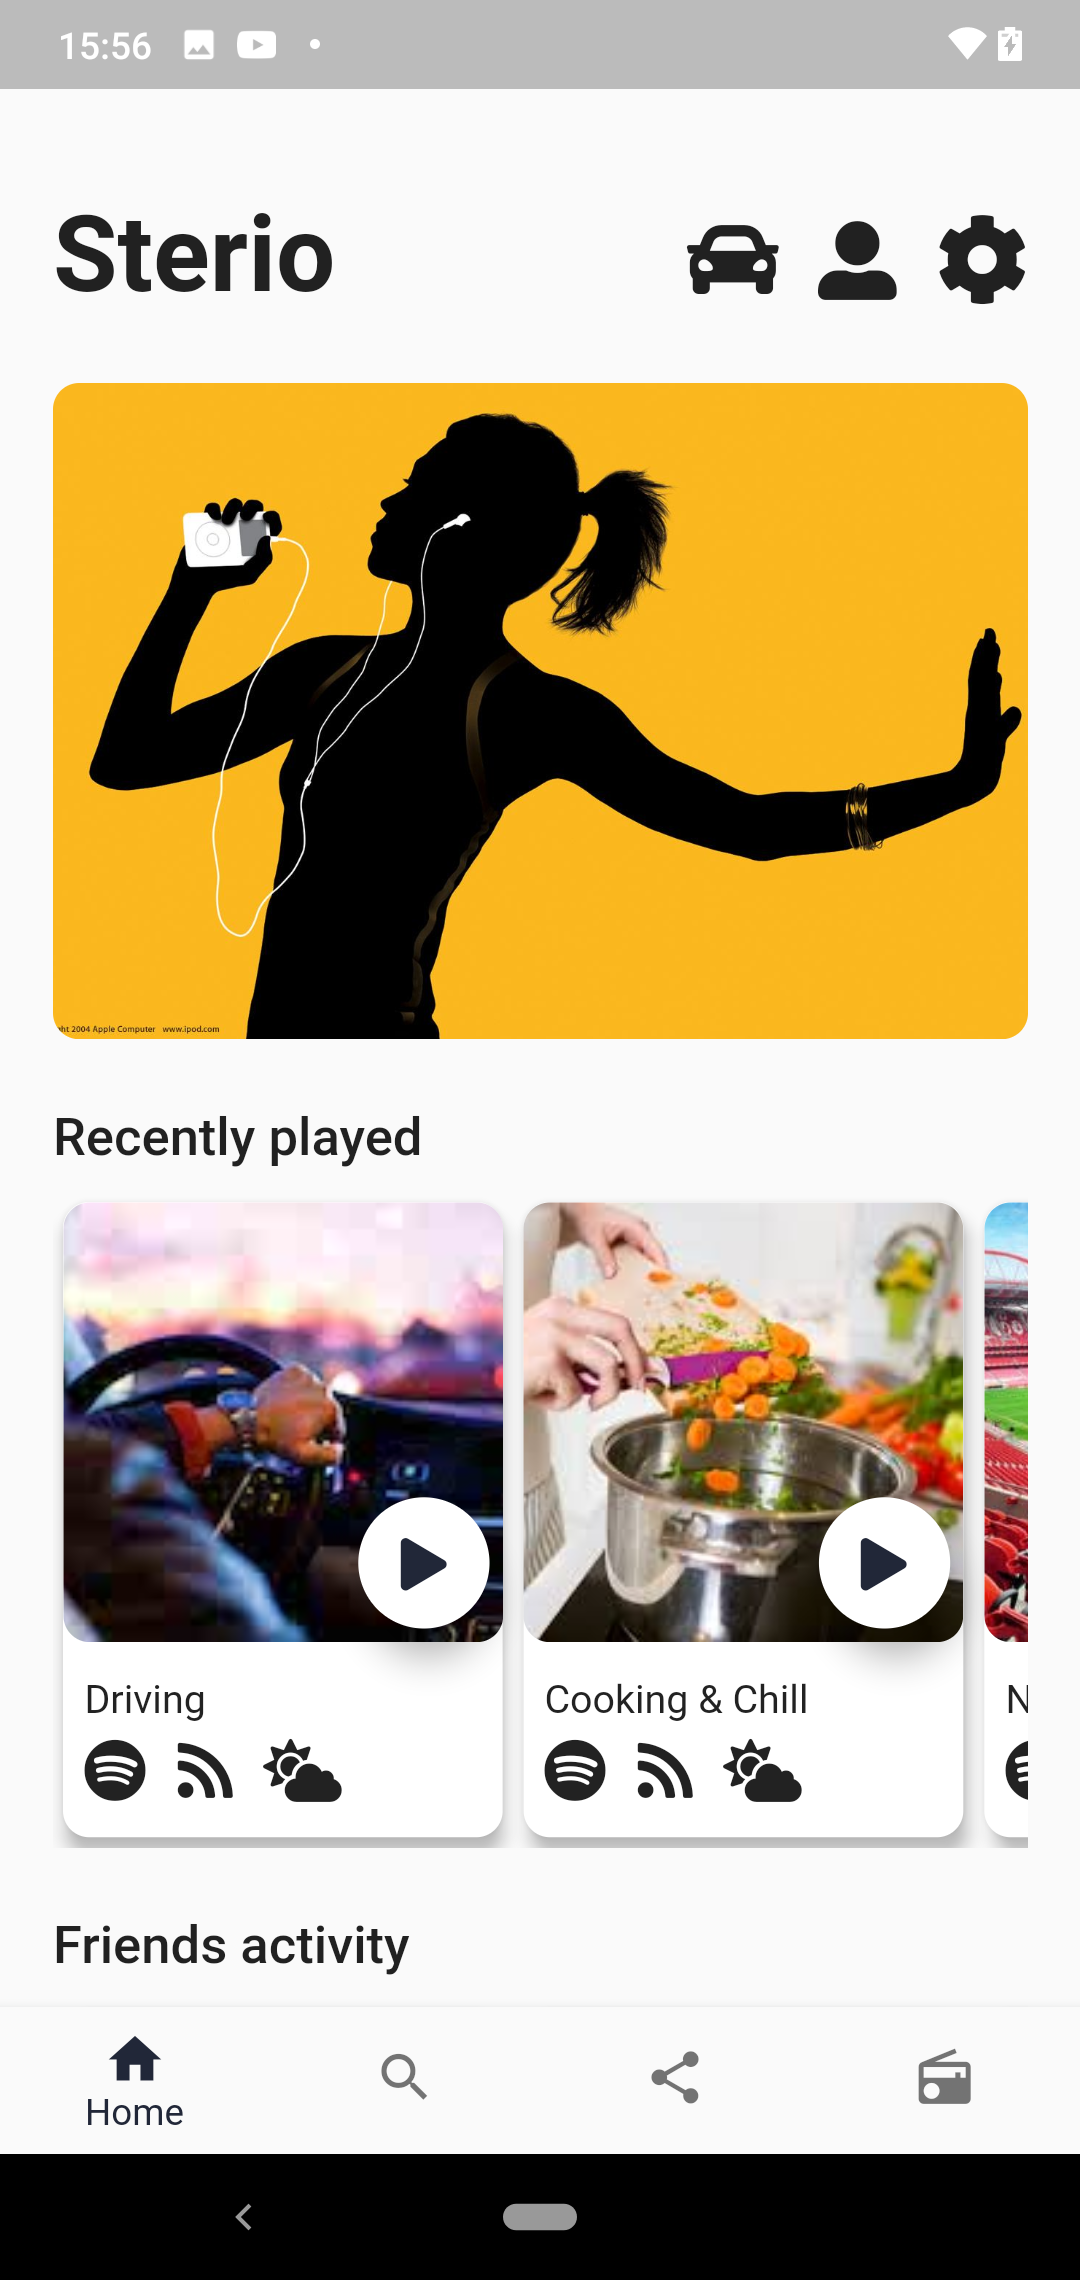
\includegraphics[width=0.29\textwidth]{./Images/screenshots/home.png}}} \qquad
	\subfigure['Search' screen]{\label{fig:searchs1}
	\frame{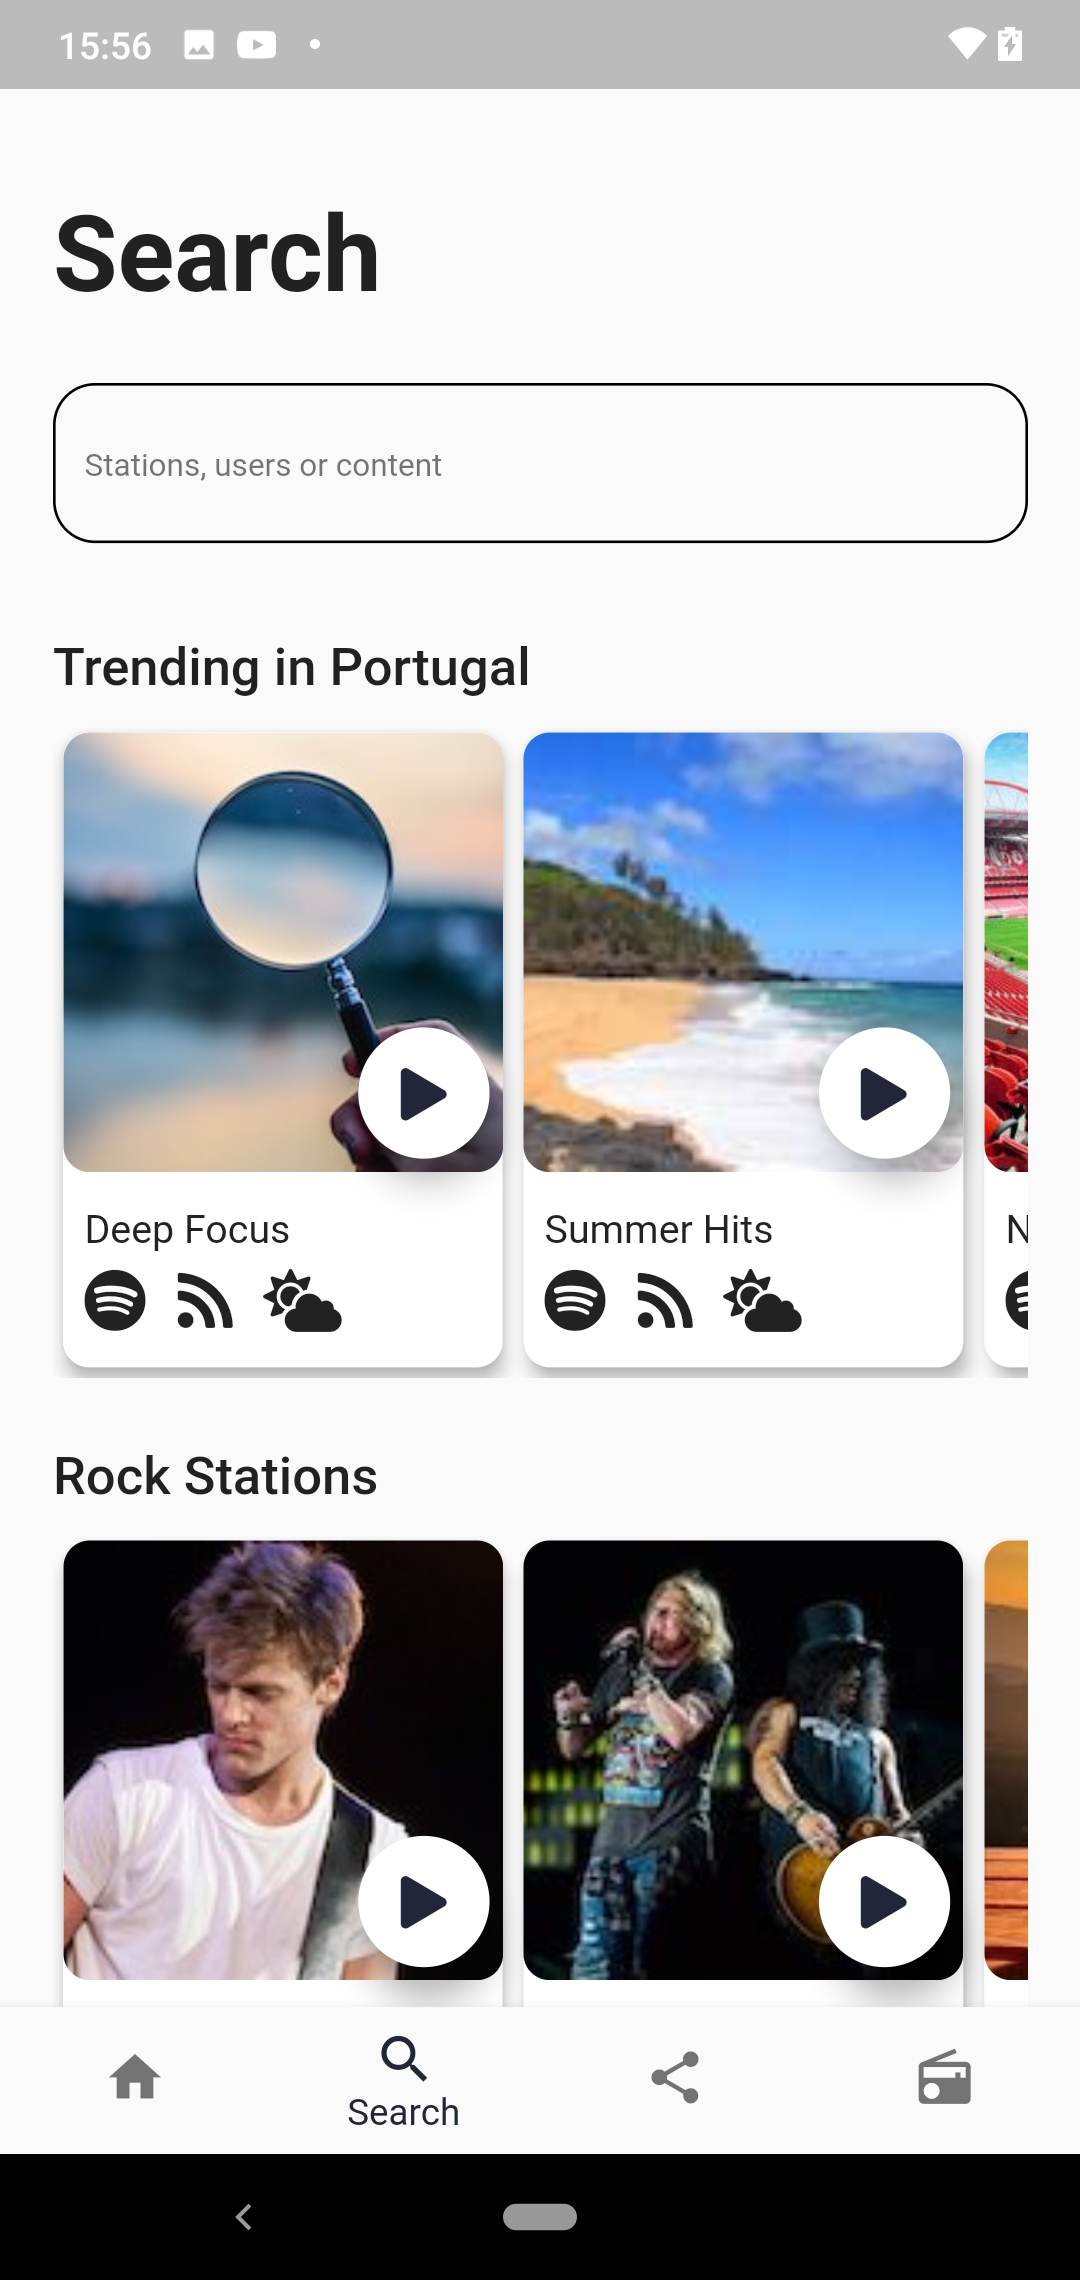
\includegraphics[width=0.29\textwidth]{./Images/screenshots/search.png}}} \qquad
	\caption{'Home' and 'Search' screens}
	\label{fig:mfp1}
\end{figure}

After logging in, the user is prompted with the 'Home' screen, shown in Figure ~\ref{fig:homes}, which is the first and most foregrounding screen of the platform. In this screen, the user can quickly play a station based on recent activity, friends activity, top charts, or other relevant information tailored to the user's taste and usability history. In this screen, the user can also change the settings and preferences of the app, as well as of the signed-in account. Finally, the user can also enter the "Car Mode" of the system, which transforms the ~\ac{UI} in a stripped-down, non-distracting, and easy way for the user to control playback while driving.

In the 'Search' screen, shown in Figure ~\ref{fig:searchs1}, the user can search for a specific station, content, or even other users to follow and check their profiles. In the same screen, listening suggestions are also shown, based on the most searched items and trending stations in a given location.

\newpage
\subsection{'Social' Screen}

The 'Social' screen aggregates all the social activity of the profiles that a given user follows. From there, users can explore what stations their followers are currently listening to, as well as to listen along to such stations (mimicking the experience of a traditional terrestrial radio station). 
\begin{figure}[htbp]
	\centering
	\subfigure[Social screen showing friends that are playing a station]{\label{fig:social1}
	\frame{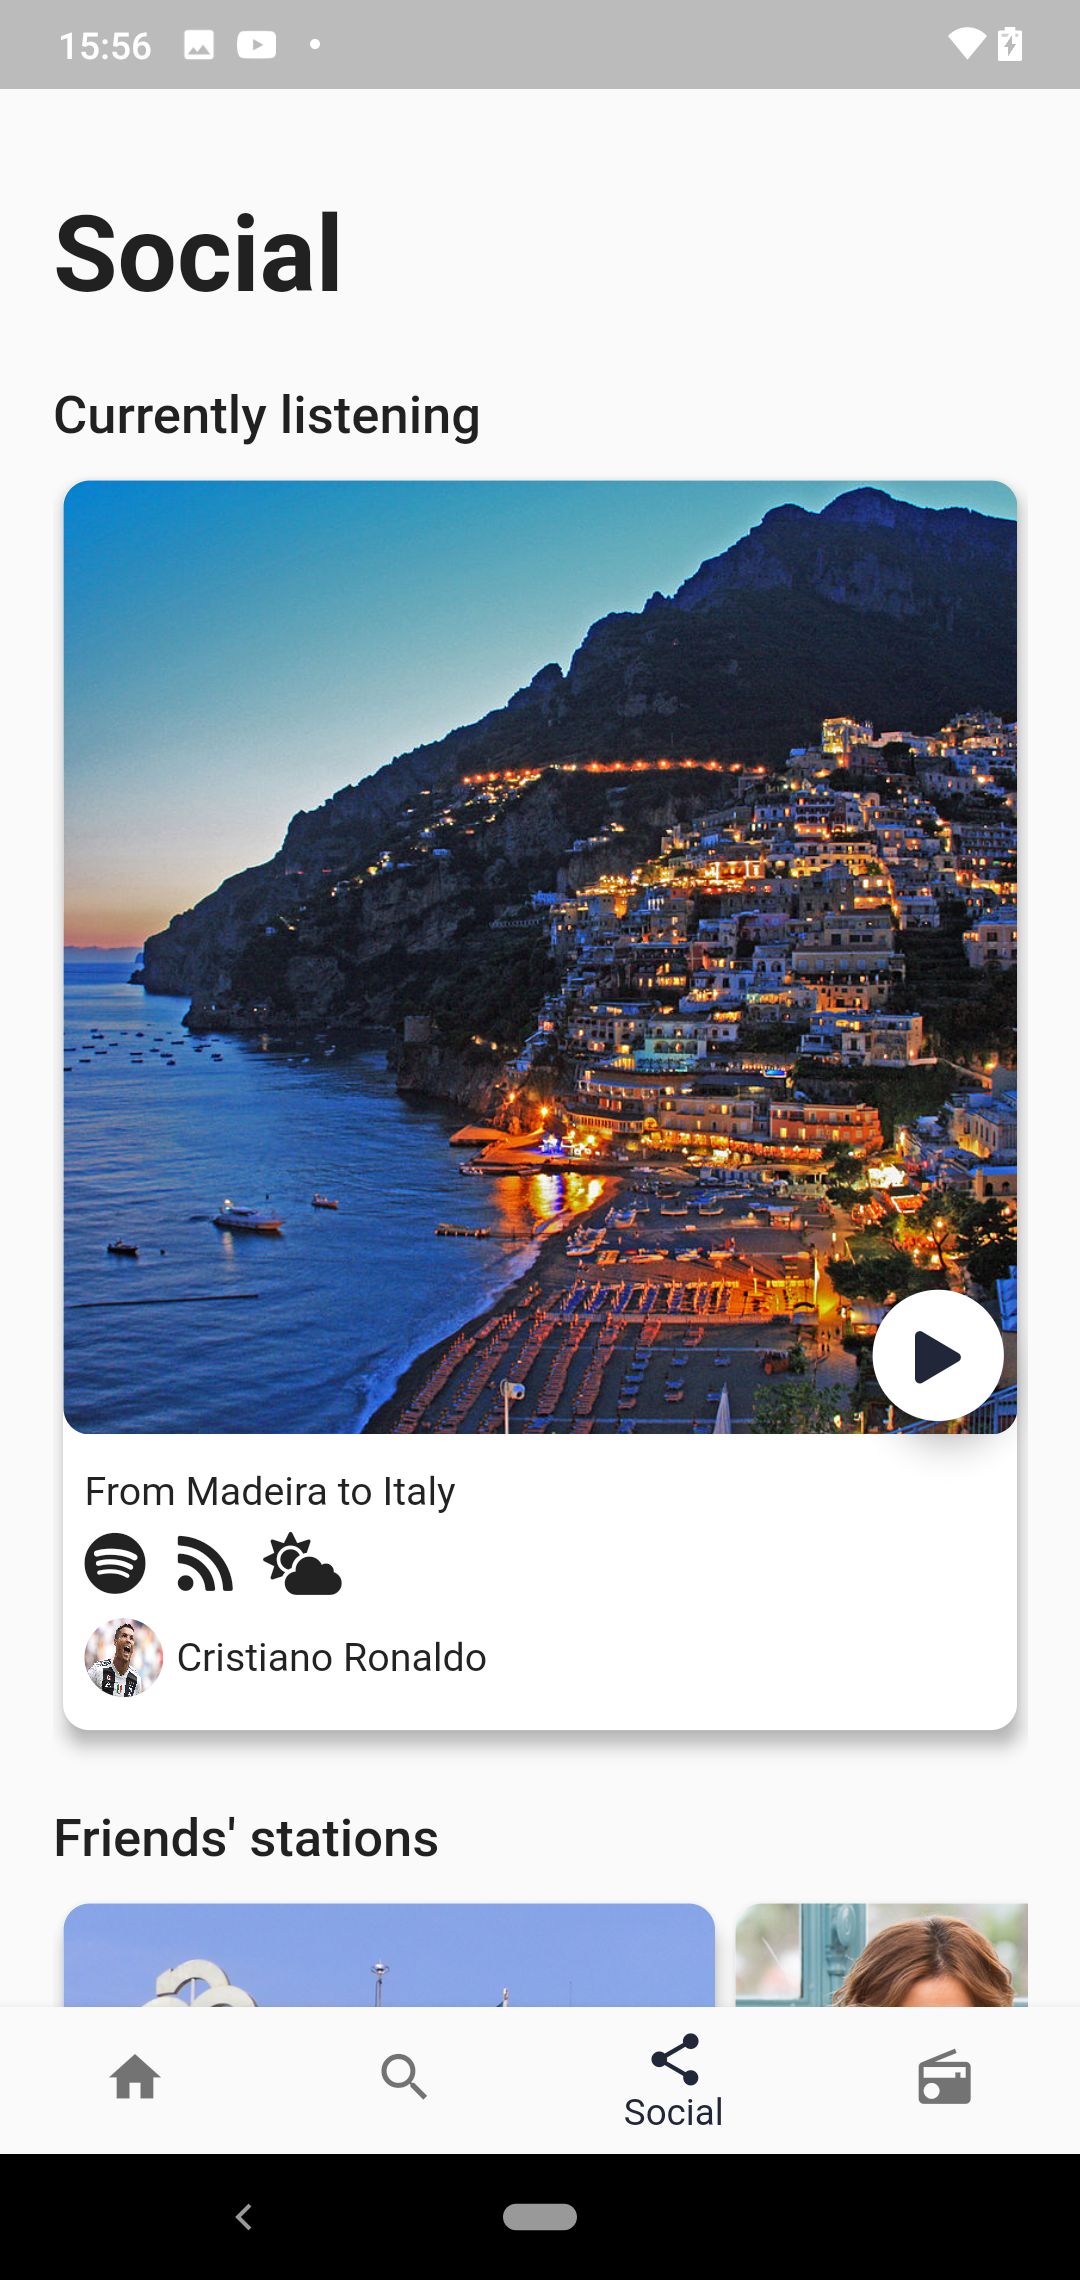
\includegraphics[width=0.29\textwidth]{./Images/screenshots/social1.png}}} \qquad
	\subfigure[Social screen with following suggestions]{\label{fig:social2}
	\frame{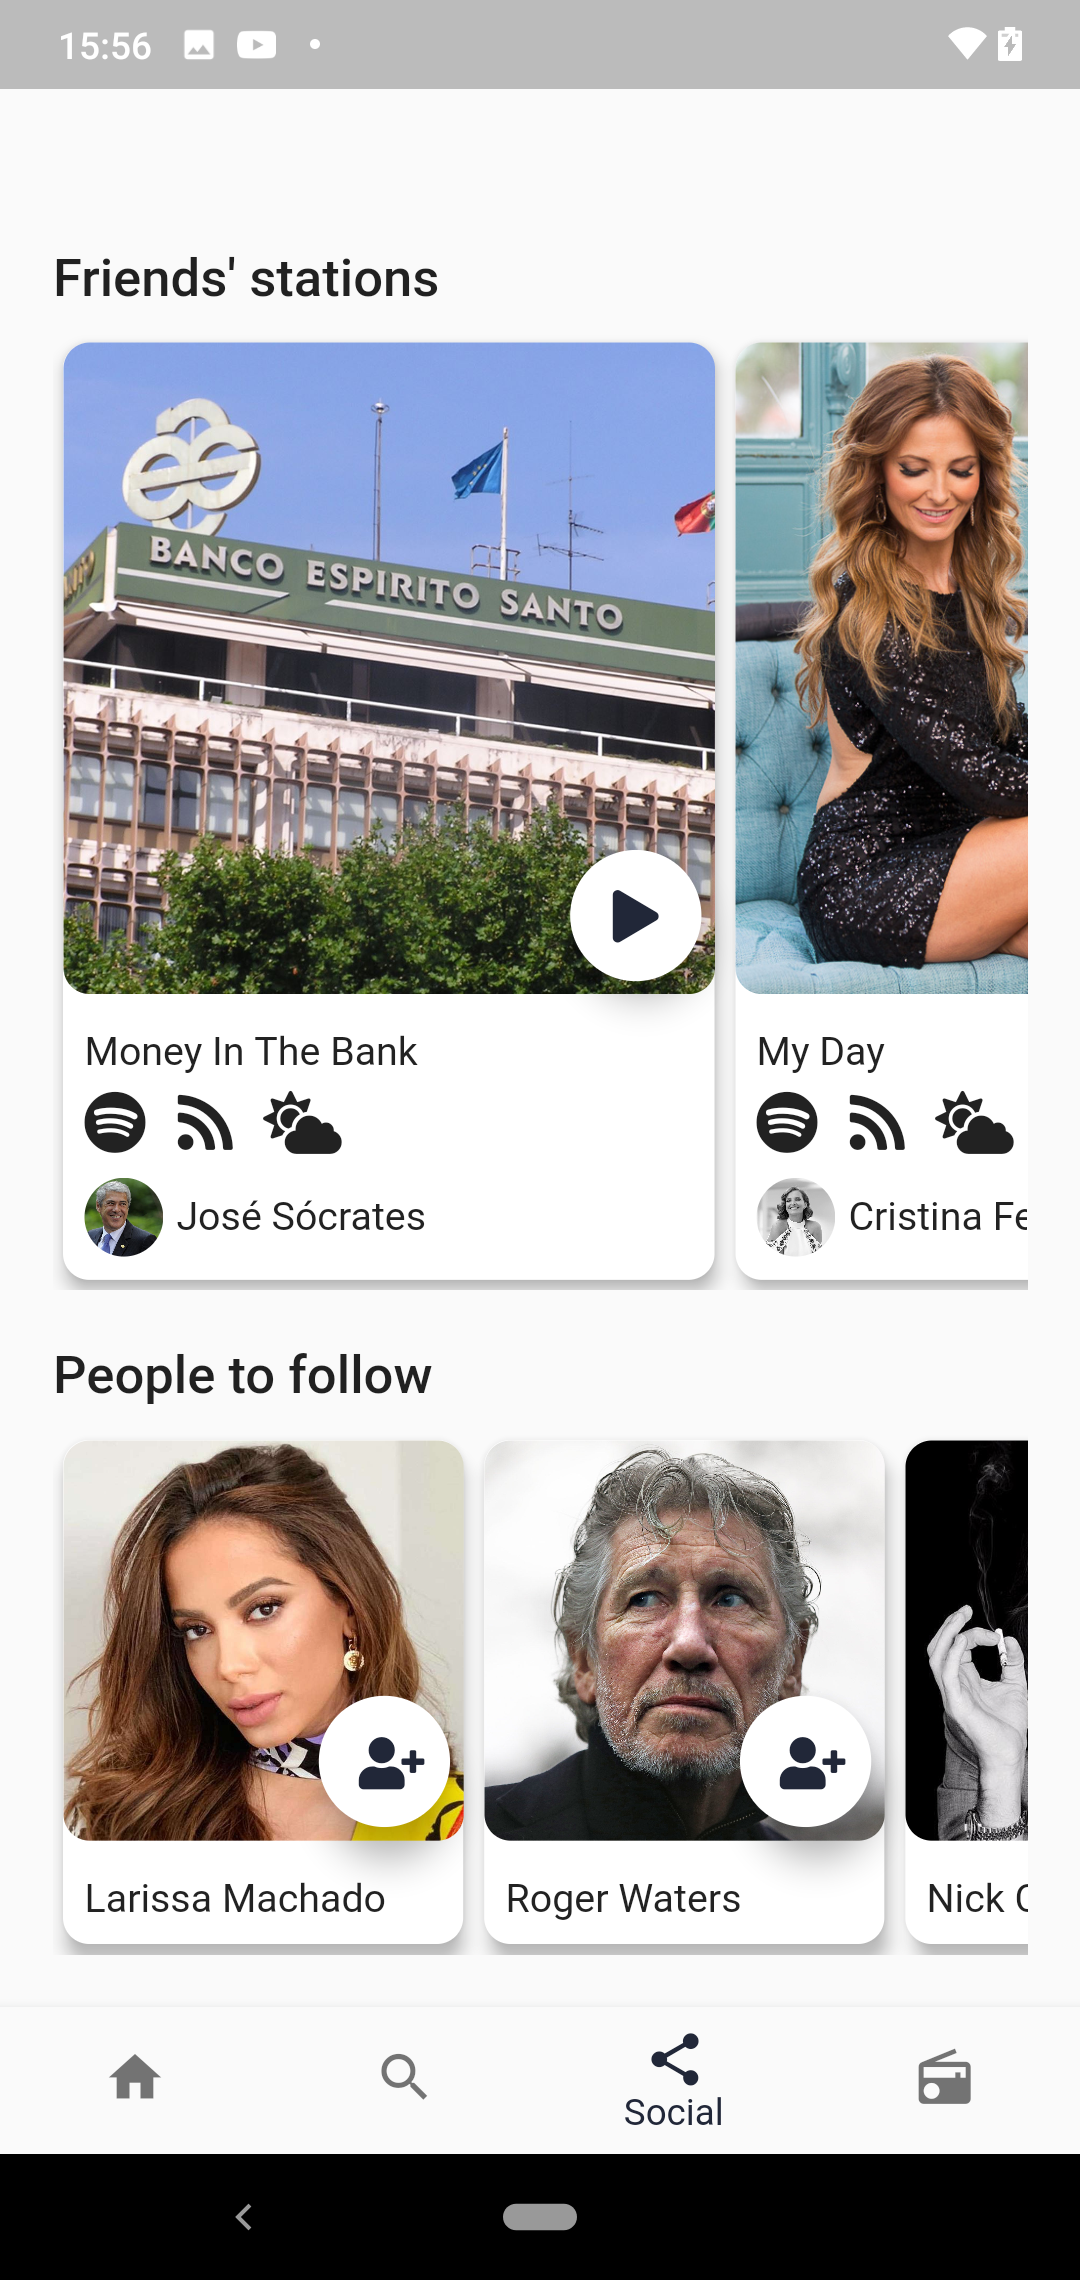
\includegraphics[width=0.29\textwidth]{./Images/screenshots/social2.png}}} \qquad
	\caption{'Social' screen}
	\label{fig:mfp1}
\end{figure}

From the same screen, users can also delve into the shared stations of their friends and family and get recommendations of profiles to follow based on their taste and friends' circle. Coinciding with a news feed of a traditional social network, users can also share and interact with shared media posts, creating a very integrated and cohesive social experience among the users of the platform.

\newpage
\subsection{'My Stations' Screen}

The last of the four main screens of the platform is the 'My Stations' screen, shown in Figure ~\ref{fig:mys}, where the user can find their own created stations, or saved stations created by other users of the platform. It acts as a 'library' of saved stations, making it easy for users to find their desired content. On the same screen, users can press the '+' red button and start the process of creating a new station, which will be added automatically to their library.

\begin{figure}[h]
\centering
\frame{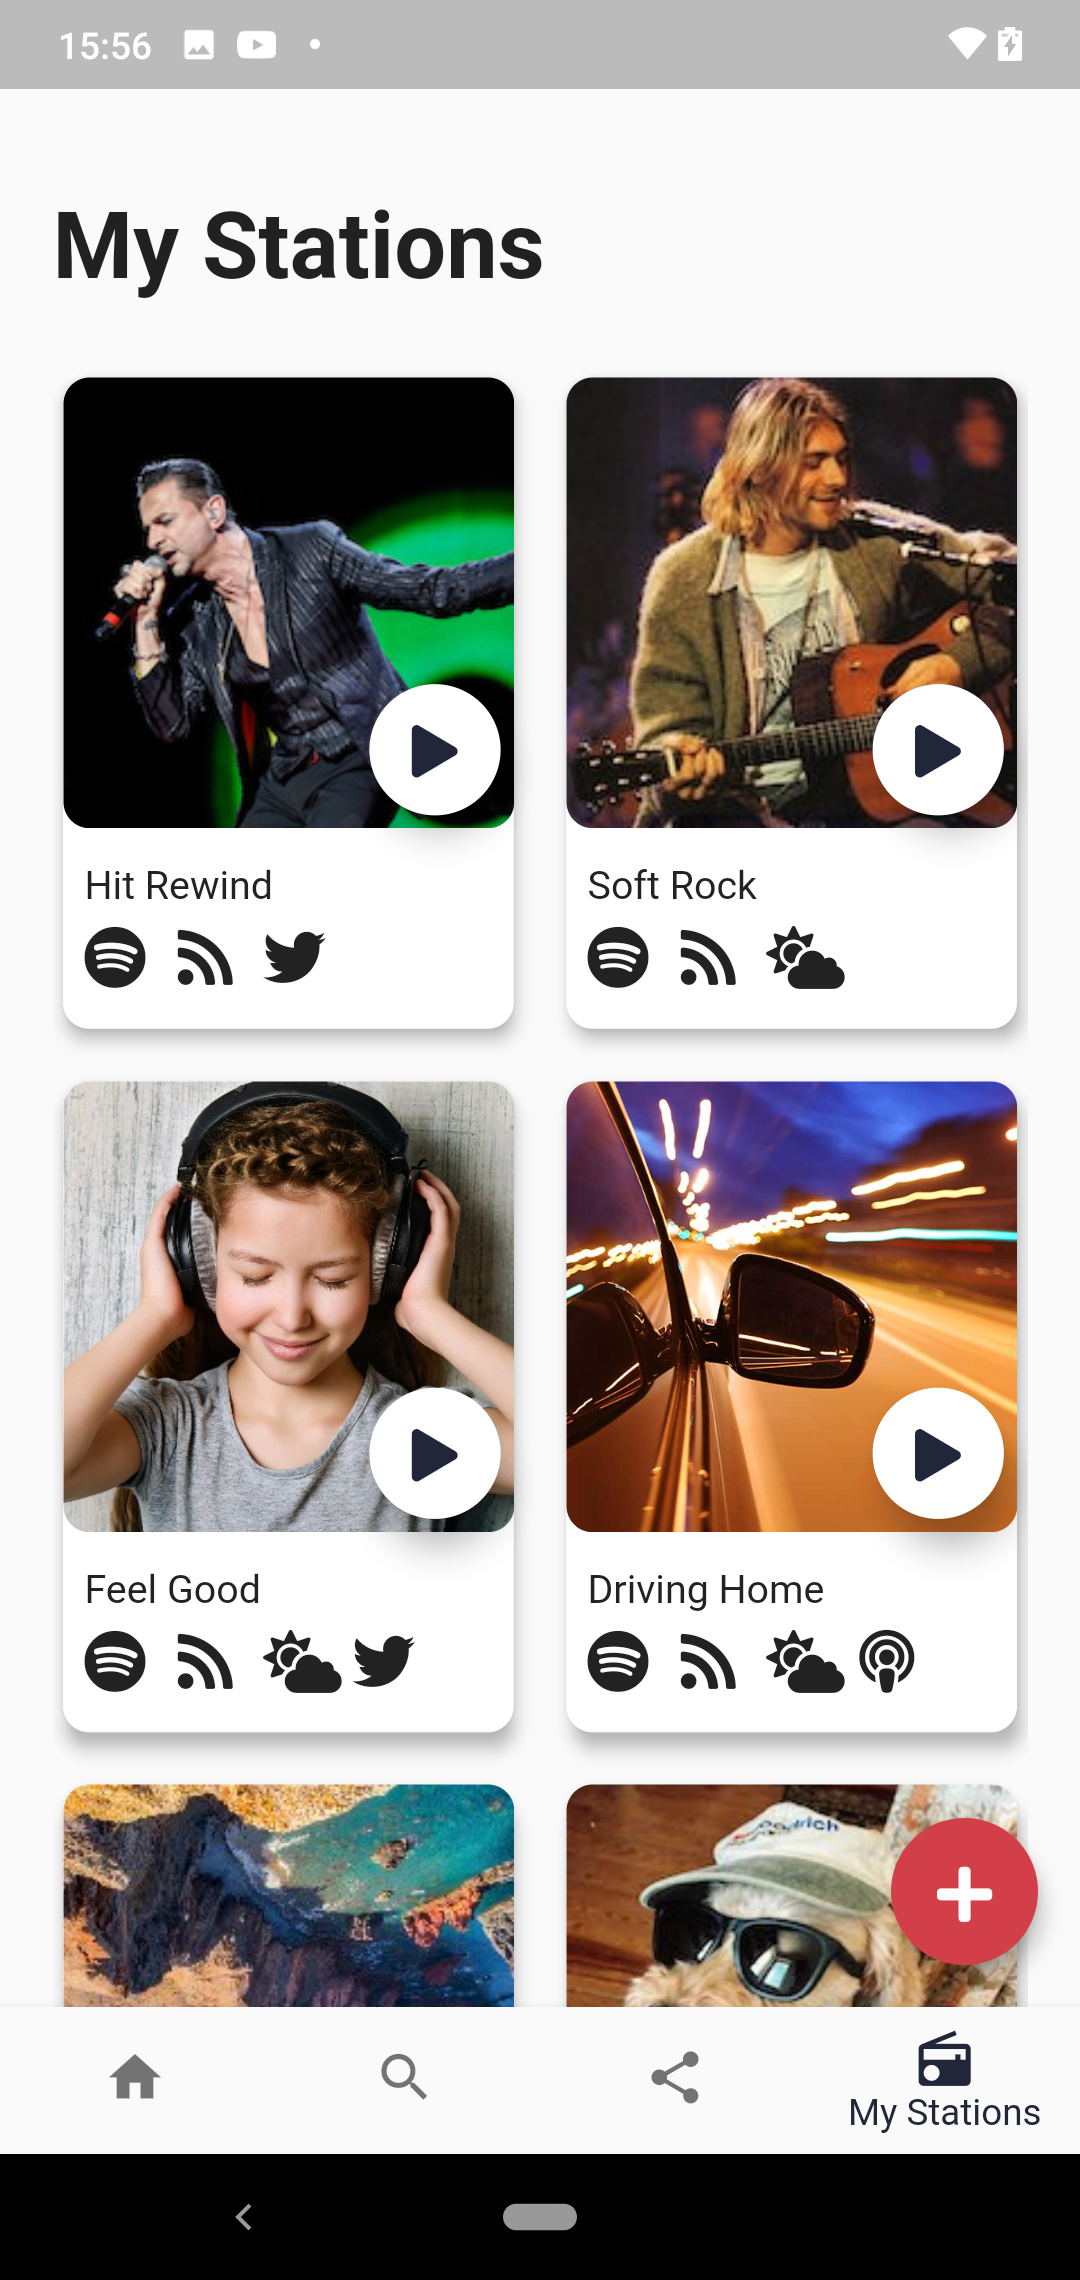
\includegraphics[width=0.29\textwidth]{./Images/screenshots/mys.png}}
\caption{'My Stations' screen}
\label{fig:mys}
\end{figure}

Each station is represented by a 'card' that displays its basic information — name, blocks, and artwork/cover. This configuration allows the user to have a glimpse of what are the contents of a given station without even entering the station's page. Furthermore, a convenient 'play' button is exposed so that users can effortlessly start playing a given station. This design is carried out across the platform's screens, creating a broad, cohesive, and consistent user experience.

All the station information is stored and loaded from the database on-demand, thus minimizing cache and offline efforts. Nevertheless, in case the user doesn't have a connection to the internet, it is possible to download and locally store a given station.


\newpage
\subsection{Creating a New Station}

\begin{figure}[htbp]
	\centering
	\subfigure[Step 1 (stations' details)]{\label{fig:ns1}
	\frame{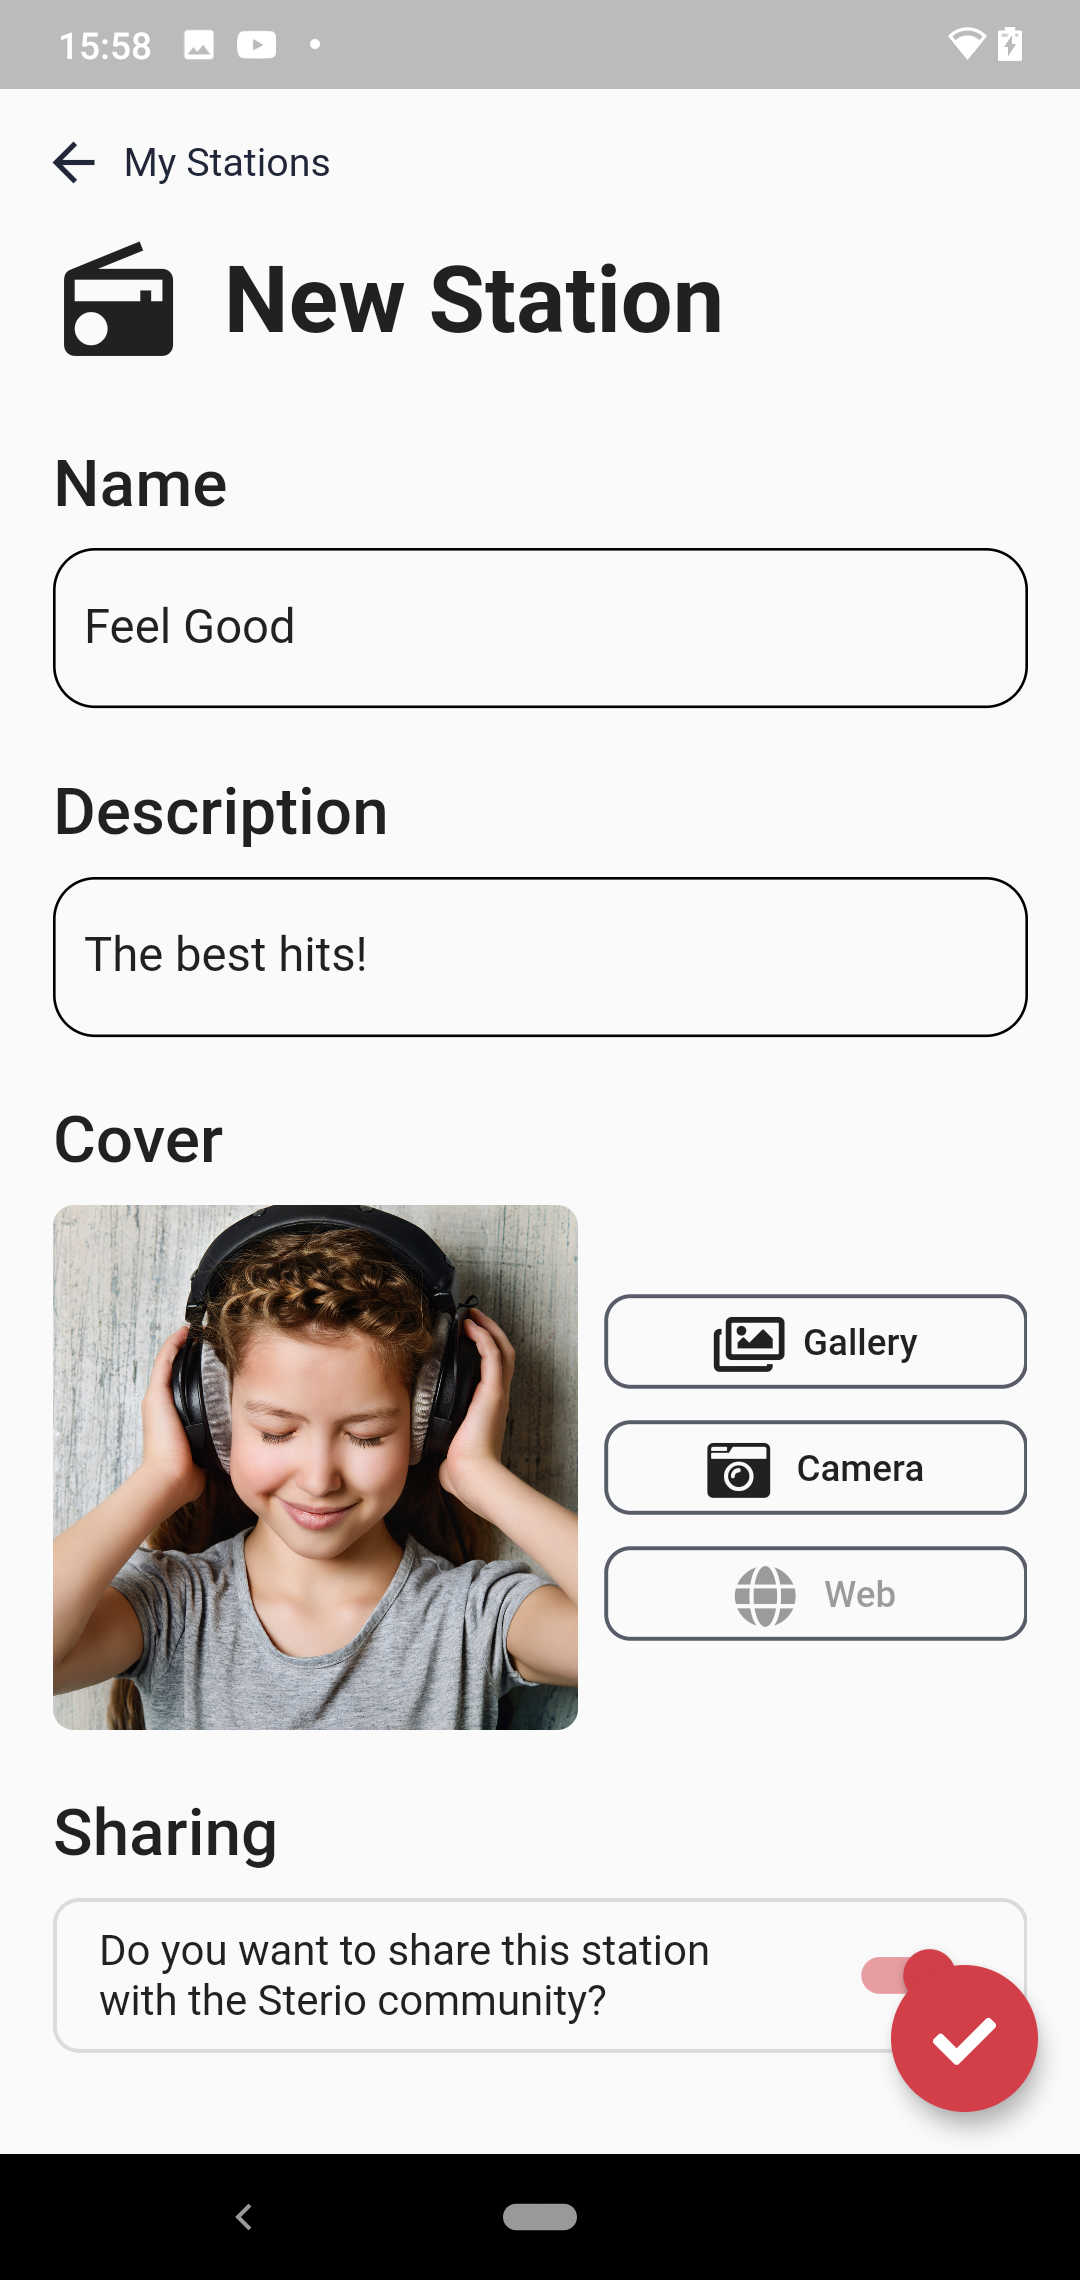
\includegraphics[width=0.29\textwidth]{./Images/screenshots/newstation1.png}}} \qquad
	\subfigure[Step 2 (adding blocks)]{\label{fig:ns2}
	\frame{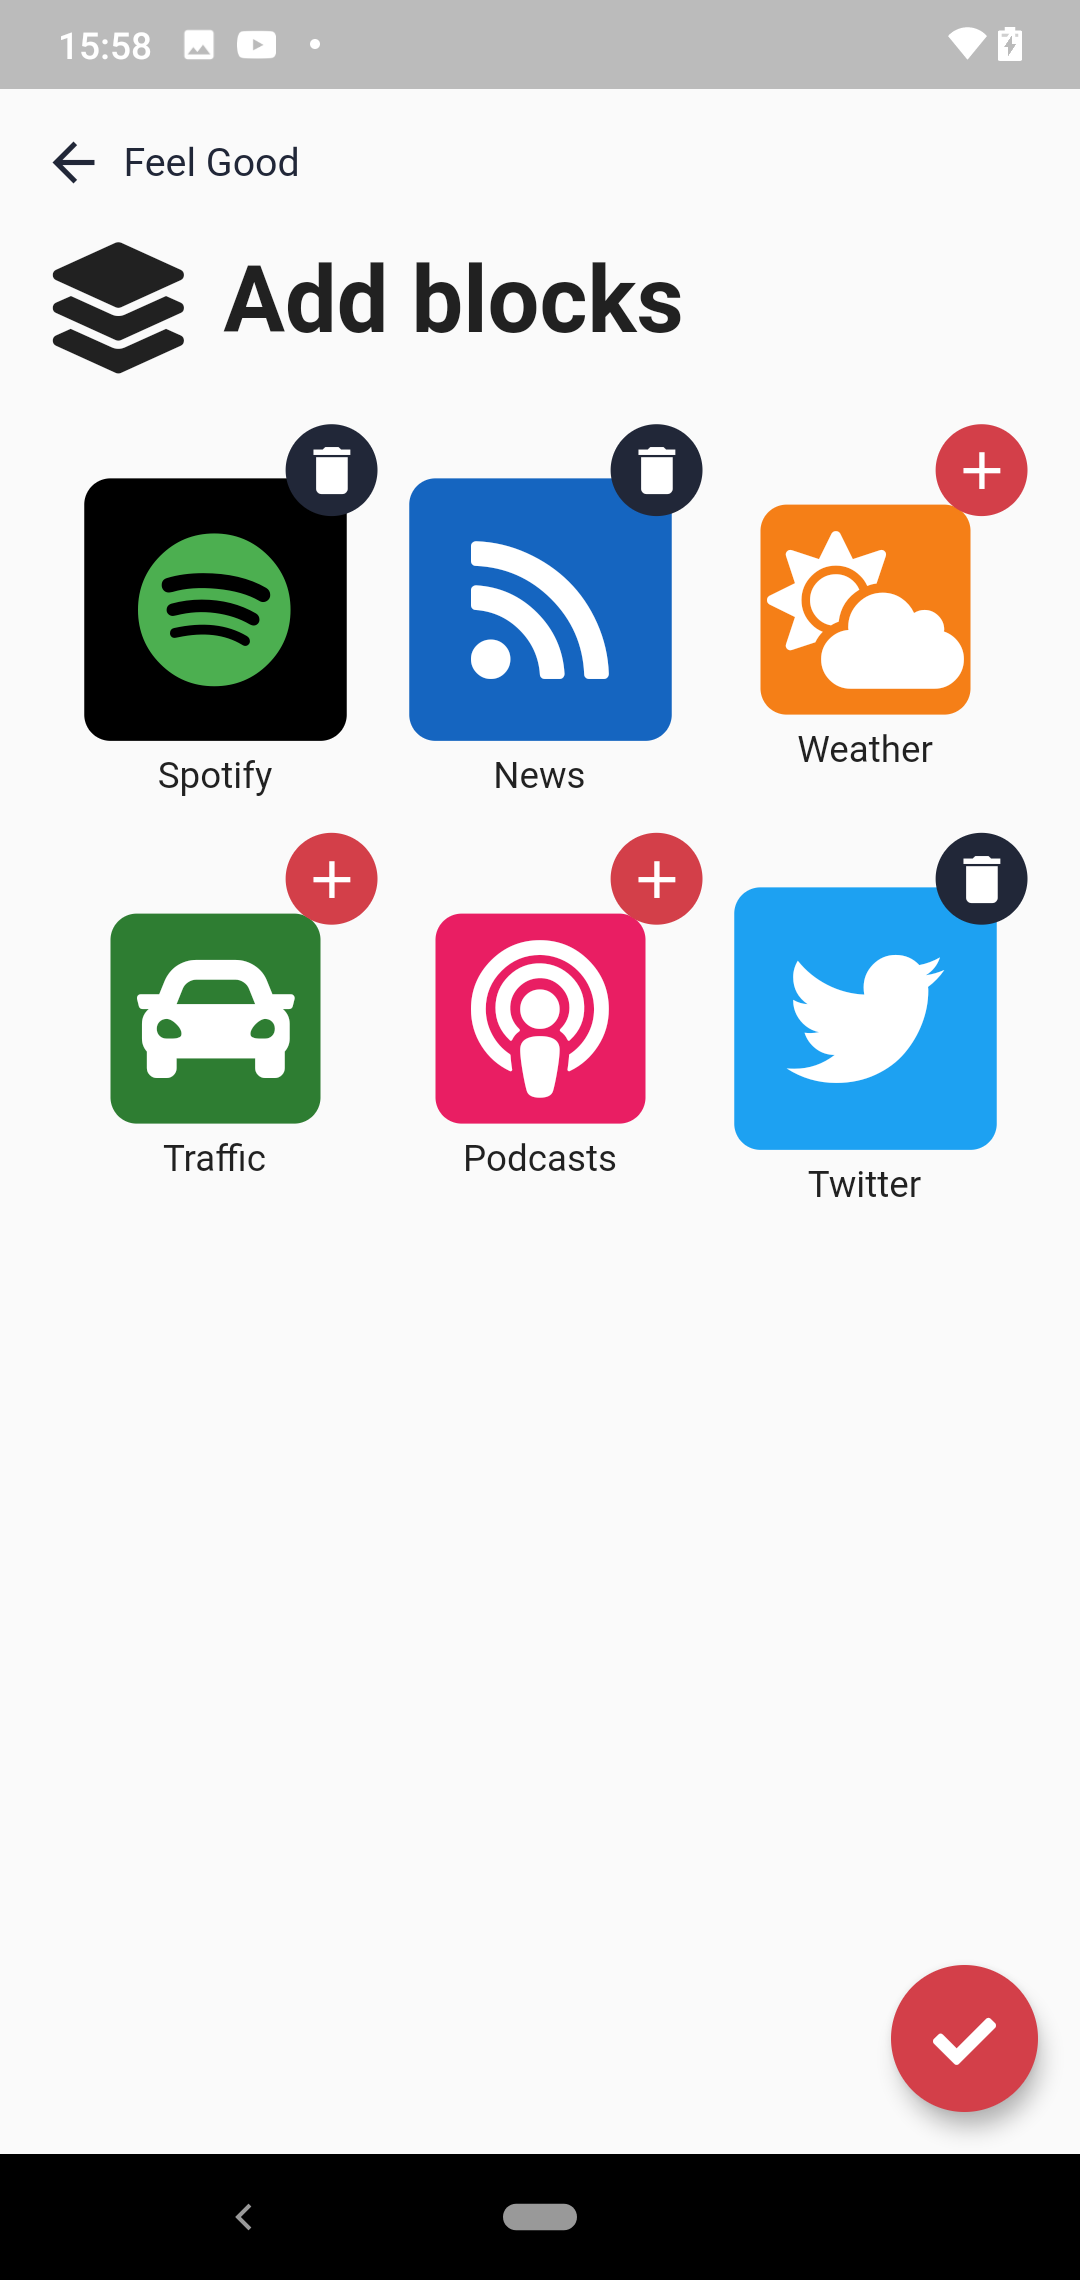
\includegraphics[width=0.29\textwidth]{./Images/screenshots/newstation2.png}}} \qquad
	\subfigure[Success screen]{\label{fig:ns3}
	\frame{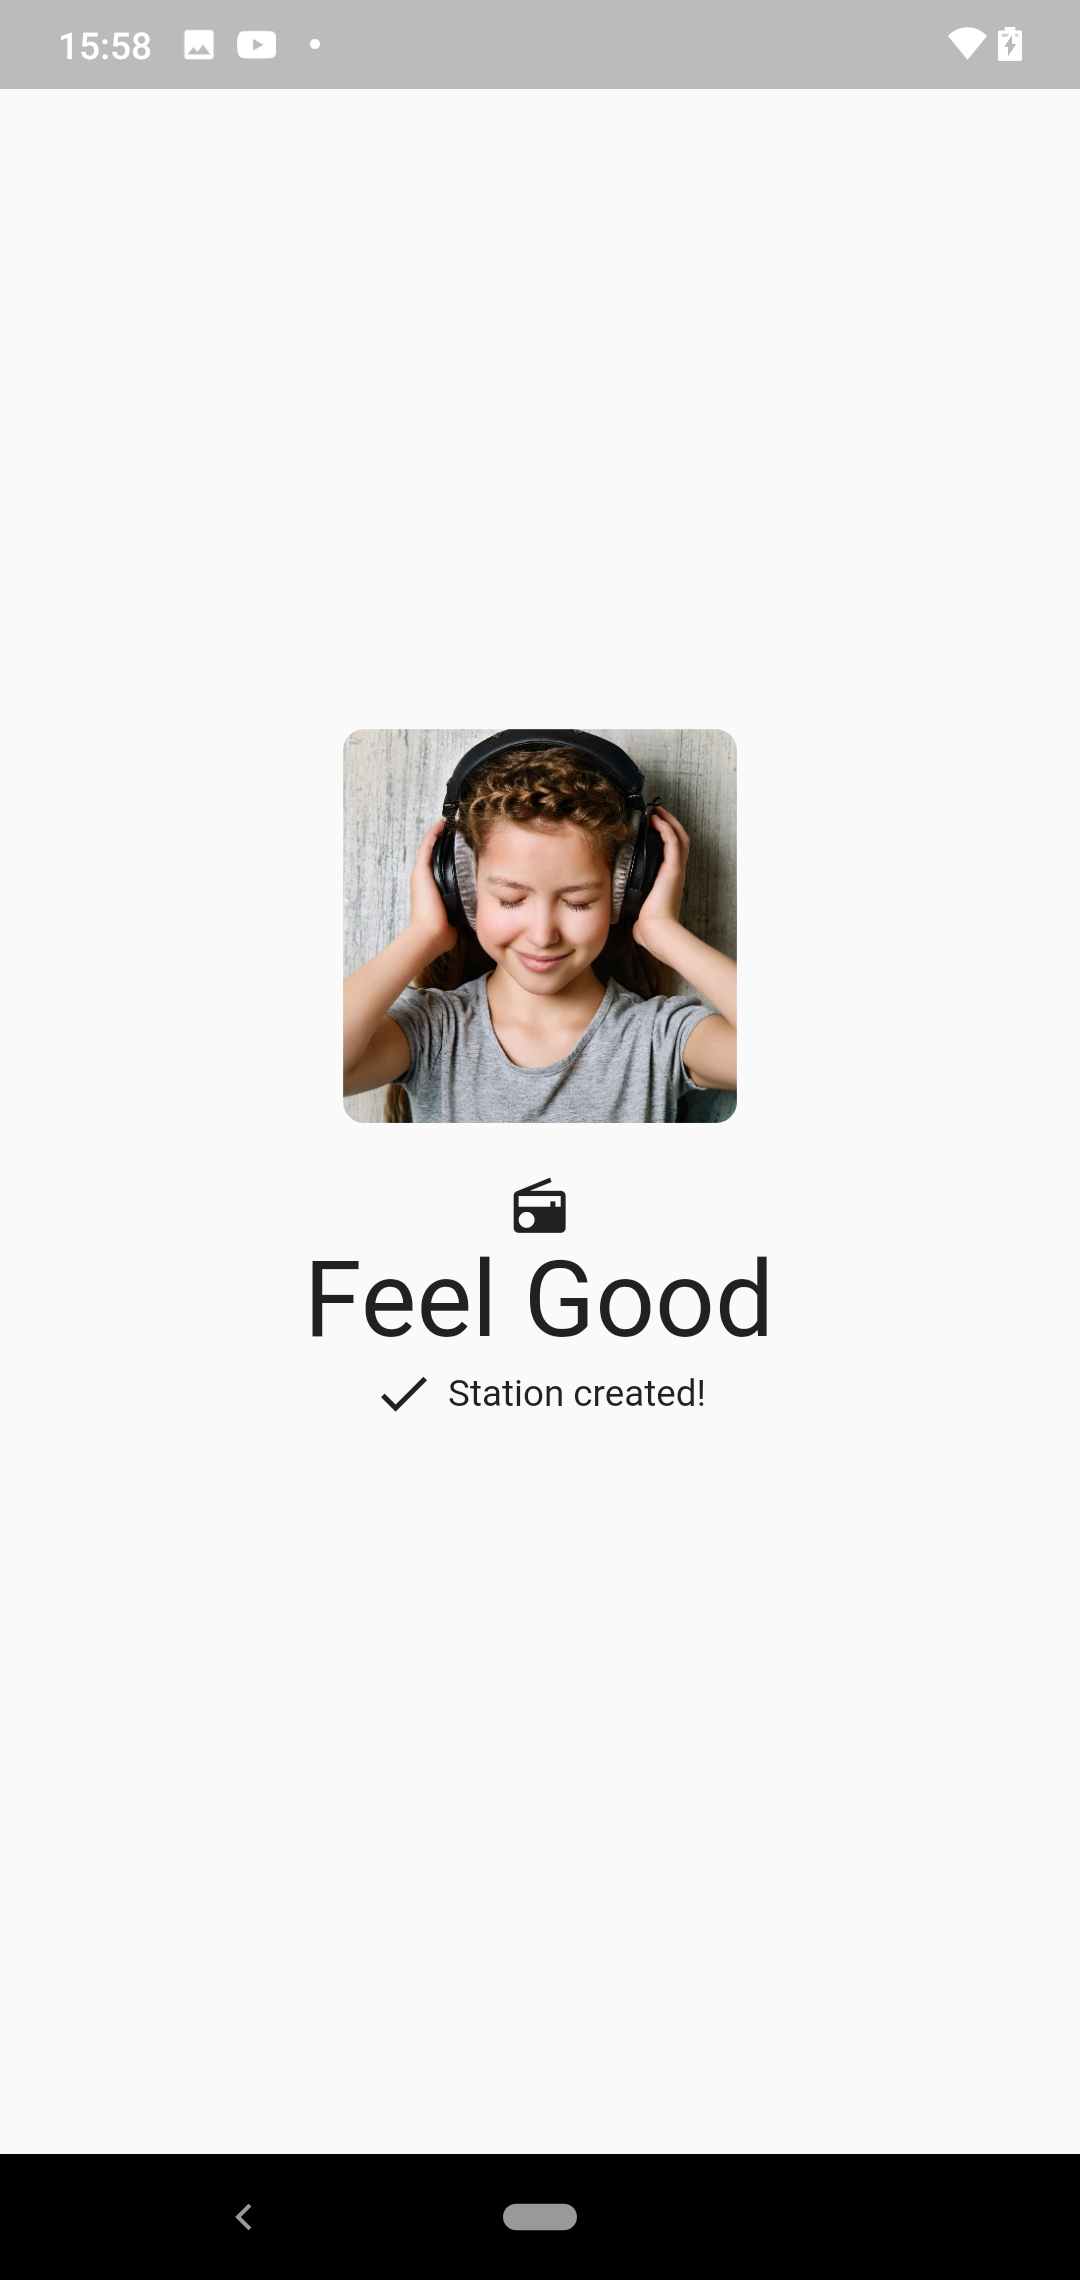
\includegraphics[width=0.29\textwidth]{./Images/screenshots/newstation3.png}}} \qquad
	\caption{Screenshots of the process of creating a new station }
	\label{fig:mfp1}
\end{figure}

From the 'My Stations' screen, users can create their custom stations. This is a simple two-step process  — first, users are requested to enter the name of the station, a brief description, a cover artwork (which can be selected from the local photo gallery, from a web search, or even from taking a picture in real-time), and a sharing option. The latter determines if the station will be kept private to the user (other users can't see the station contents nor play it), or if it is shared with the community of the platform's users. The screen where the user is prompted to enter this information is shown in Figure ~\ref{fig:ns1}.


The second and final step of the creation process of a new station is the selection of 'blocks'. Each 'block' represents a service or source of information that can be added to the station playback. A simple screen, represented in Figure ~\ref{fig:ns2}, is shown to the user so that they can select the desired blocks simply and intuitively. After the user is elated with their choices, the created station information is stored in the database, and if such a process is successful, a confirmation screen  (represented in Figure ~\ref{fig:ns3}) is shown to the user. Finally, the user is redirected to the 'My Stations' screen (Figure ~\ref{fig:mys}), where the newly created station is now listed.

\newpage
\subsection{Configuring and Customizing a Station}

\begin{figure}[htbp]
	\centering
	\subfigure[Blocks screen]{\label{fig:s1}
	\frame{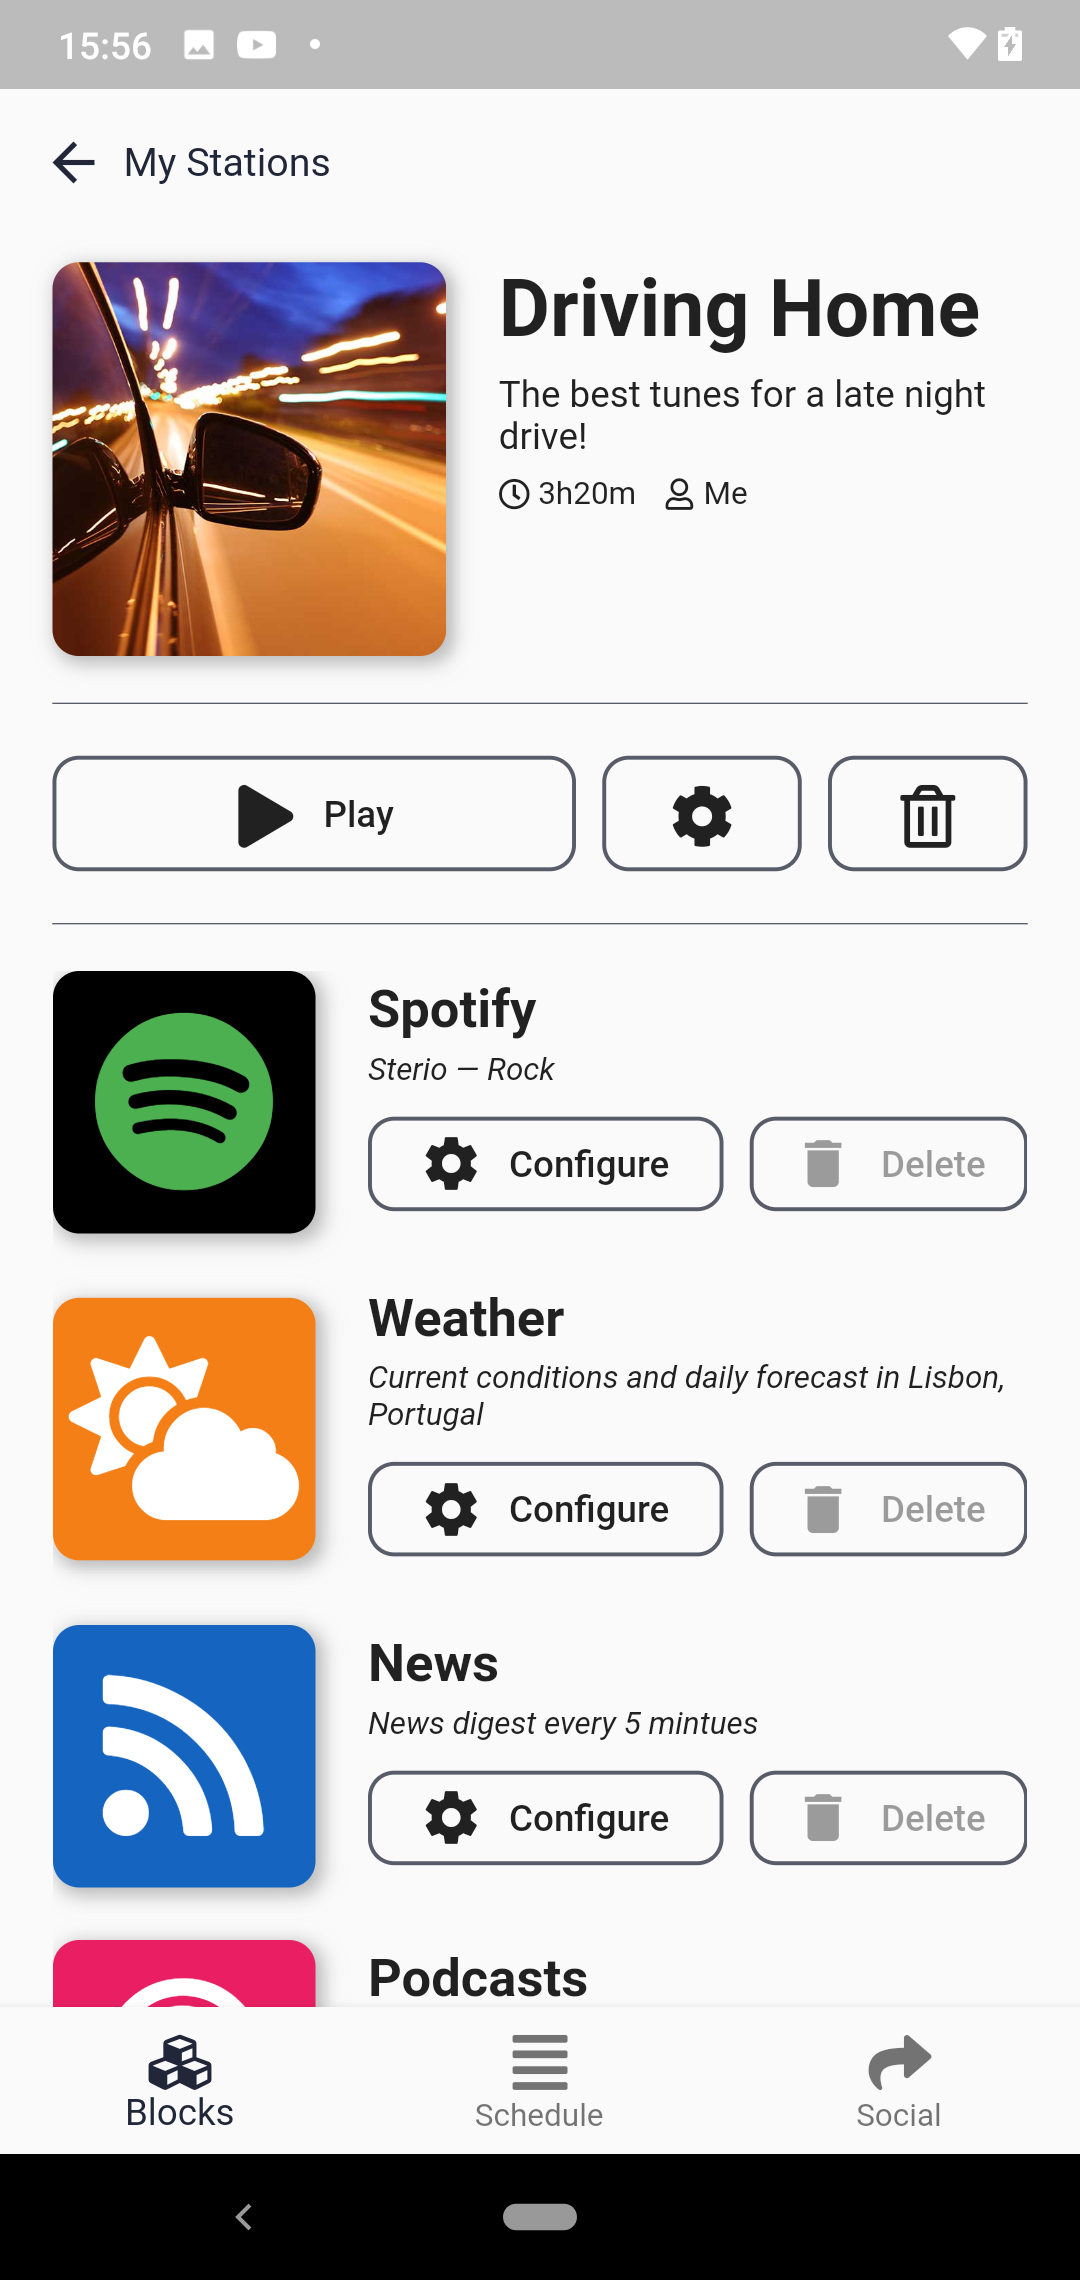
\includegraphics[width=0.29\textwidth]{./Images/screenshots/station1.png}}} \qquad
	\subfigure[Schedule screen screen]{\label{fig:s2}
	\frame{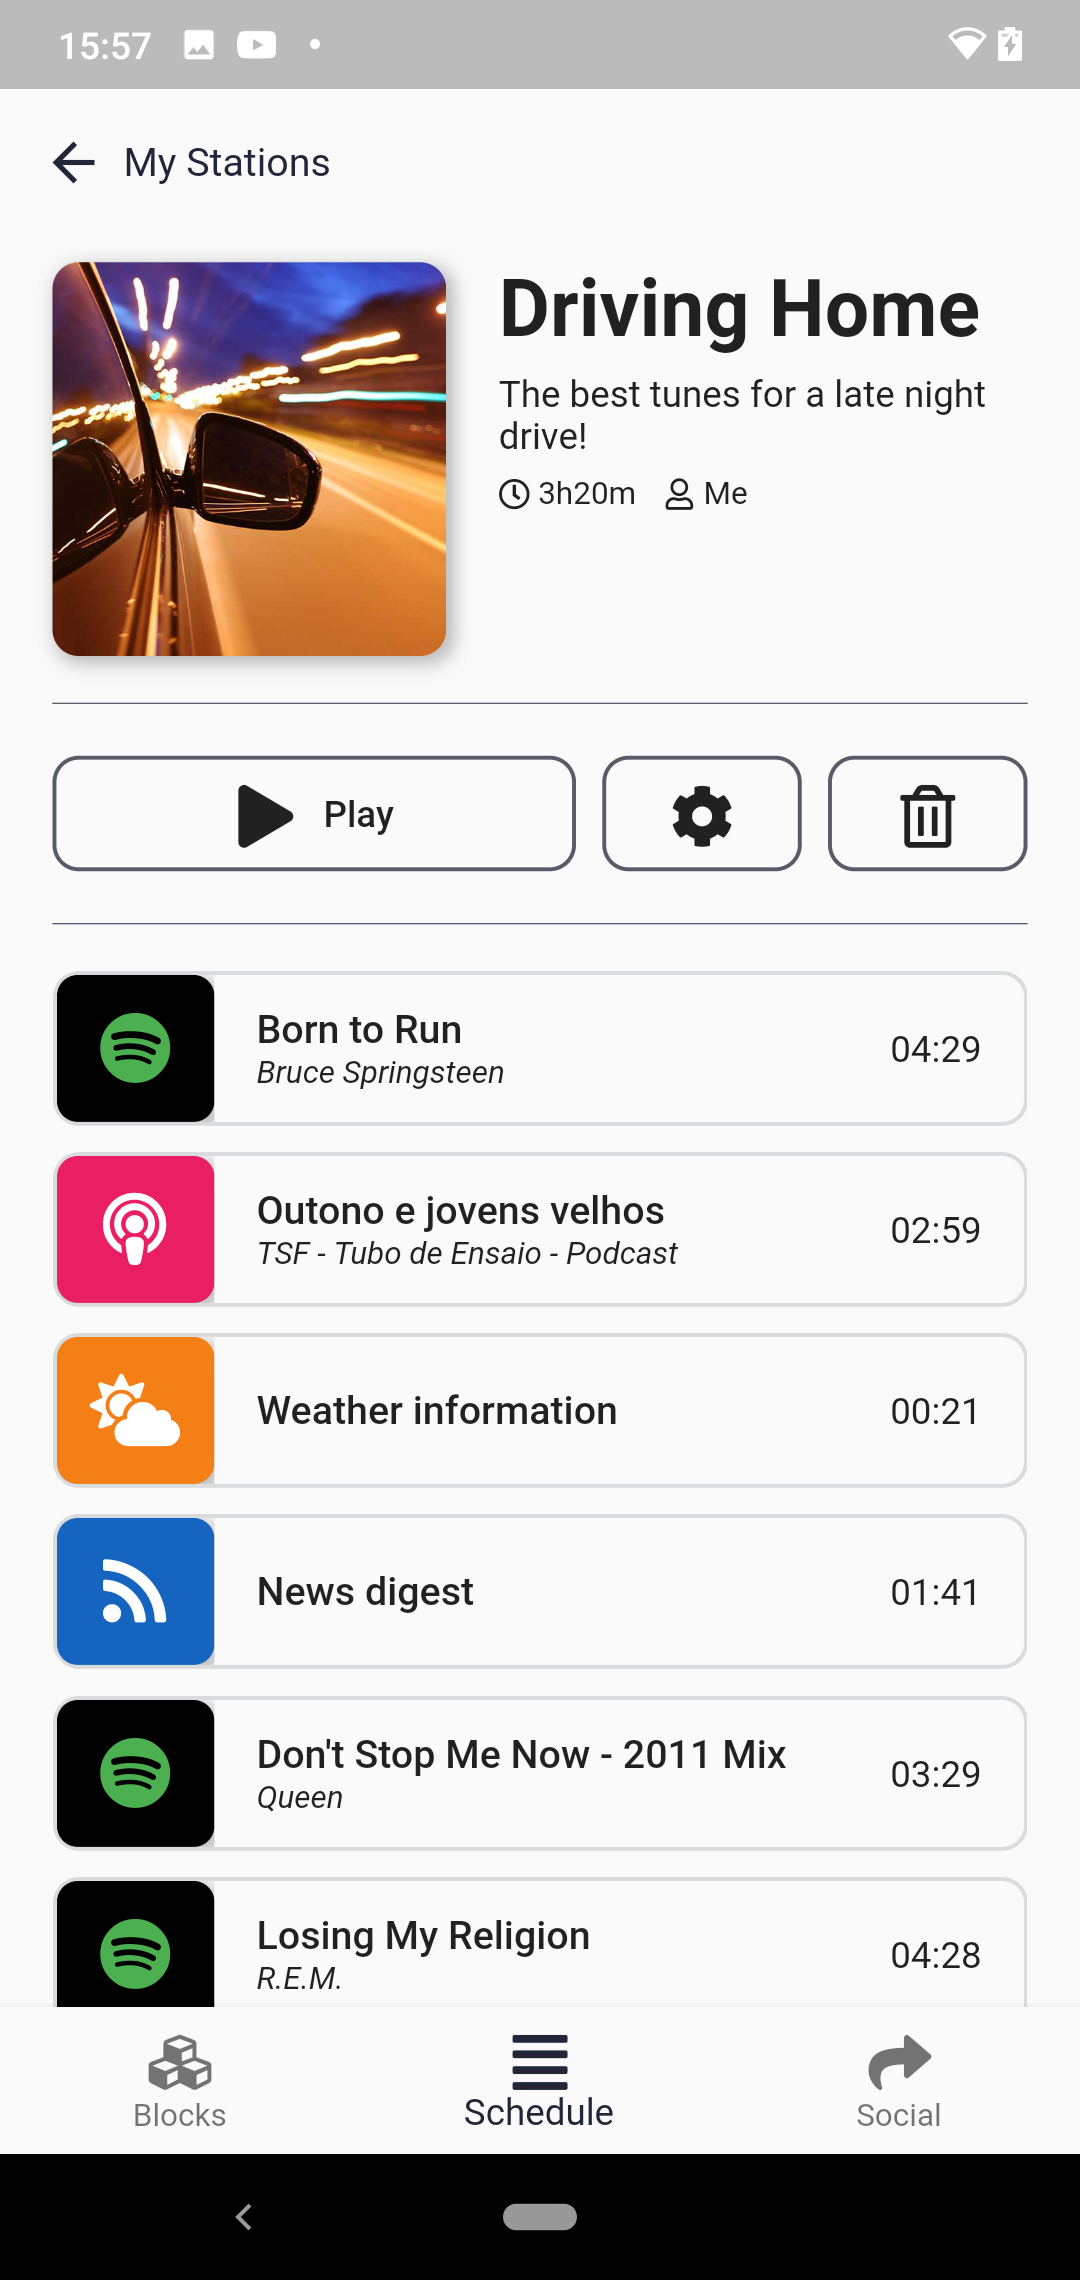
\includegraphics[width=0.29\textwidth]{./Images/screenshots/station2.png}}} \qquad
	\caption{'Driving Home' station screens}
	\label{fig:mfp1}
\end{figure}



Each station has its dedicated page, where the user can explore and customize all aspects and features of it. This screen is divided into three sub-screens that fill the latter half of the canvas — the 'blocks', 'schedule', and 'social' screen.

The 'blocks' screen showcases all the added blocks of the station. In this sub-screen, it is possible to configure, add, or remove individual blocks. The 'schedule' screen presents visually the order in which the content inserted from each block will be played. The user can fully customize the order and also remove individual elements. Finally, in the 'social' screen — which is only displayed if the creator of the station allowed its sharing with the community — users can see the profiles that follow the station, as well to accept or decline any changes that other users have suggested to the station's content.

On the first half of the screen, users can examine the station's name, description, artwork cover, duration, and creator (or creators). There, users can also start playing the station, enter its settings screen (where it is possible to adjust some configurations, such as the used text-to-speech voice), or delete the given station.

In the following subsections, we explain in greater detail the logical and technical implementations of four of the available station blocks — Spotify, Podcasts, Weather, and News. 


\subsubsection{Spotify and Podcasts}
\label{sub:spotify}

The Spotify block serves as the main connection to the music streaming service. From there, users can explore their music library and select their desired content (that could be represented in the form of a single song, artist, album, or even full playlists). To make it easier for users to add content, the recently played songs from the user's Spotify account are also displayed. Users can select an unlimited number of items, which are added to the station schedule automatically and in the order of their choice.

As mentioned in Section ~\ref{chap:relatedwork}, Spotify also provides access to a growing library of podcasts, which the user can also add to their stations. Nevertheless, although the provider of both music and podcasts is the mentioned music streaming service, a separate block dedicated to Podcasts was created.

\begin{figure}[htbp]
	\centering
	\subfigure[Spotify main configuration screen]{\label{fig:spotify1}
	\frame{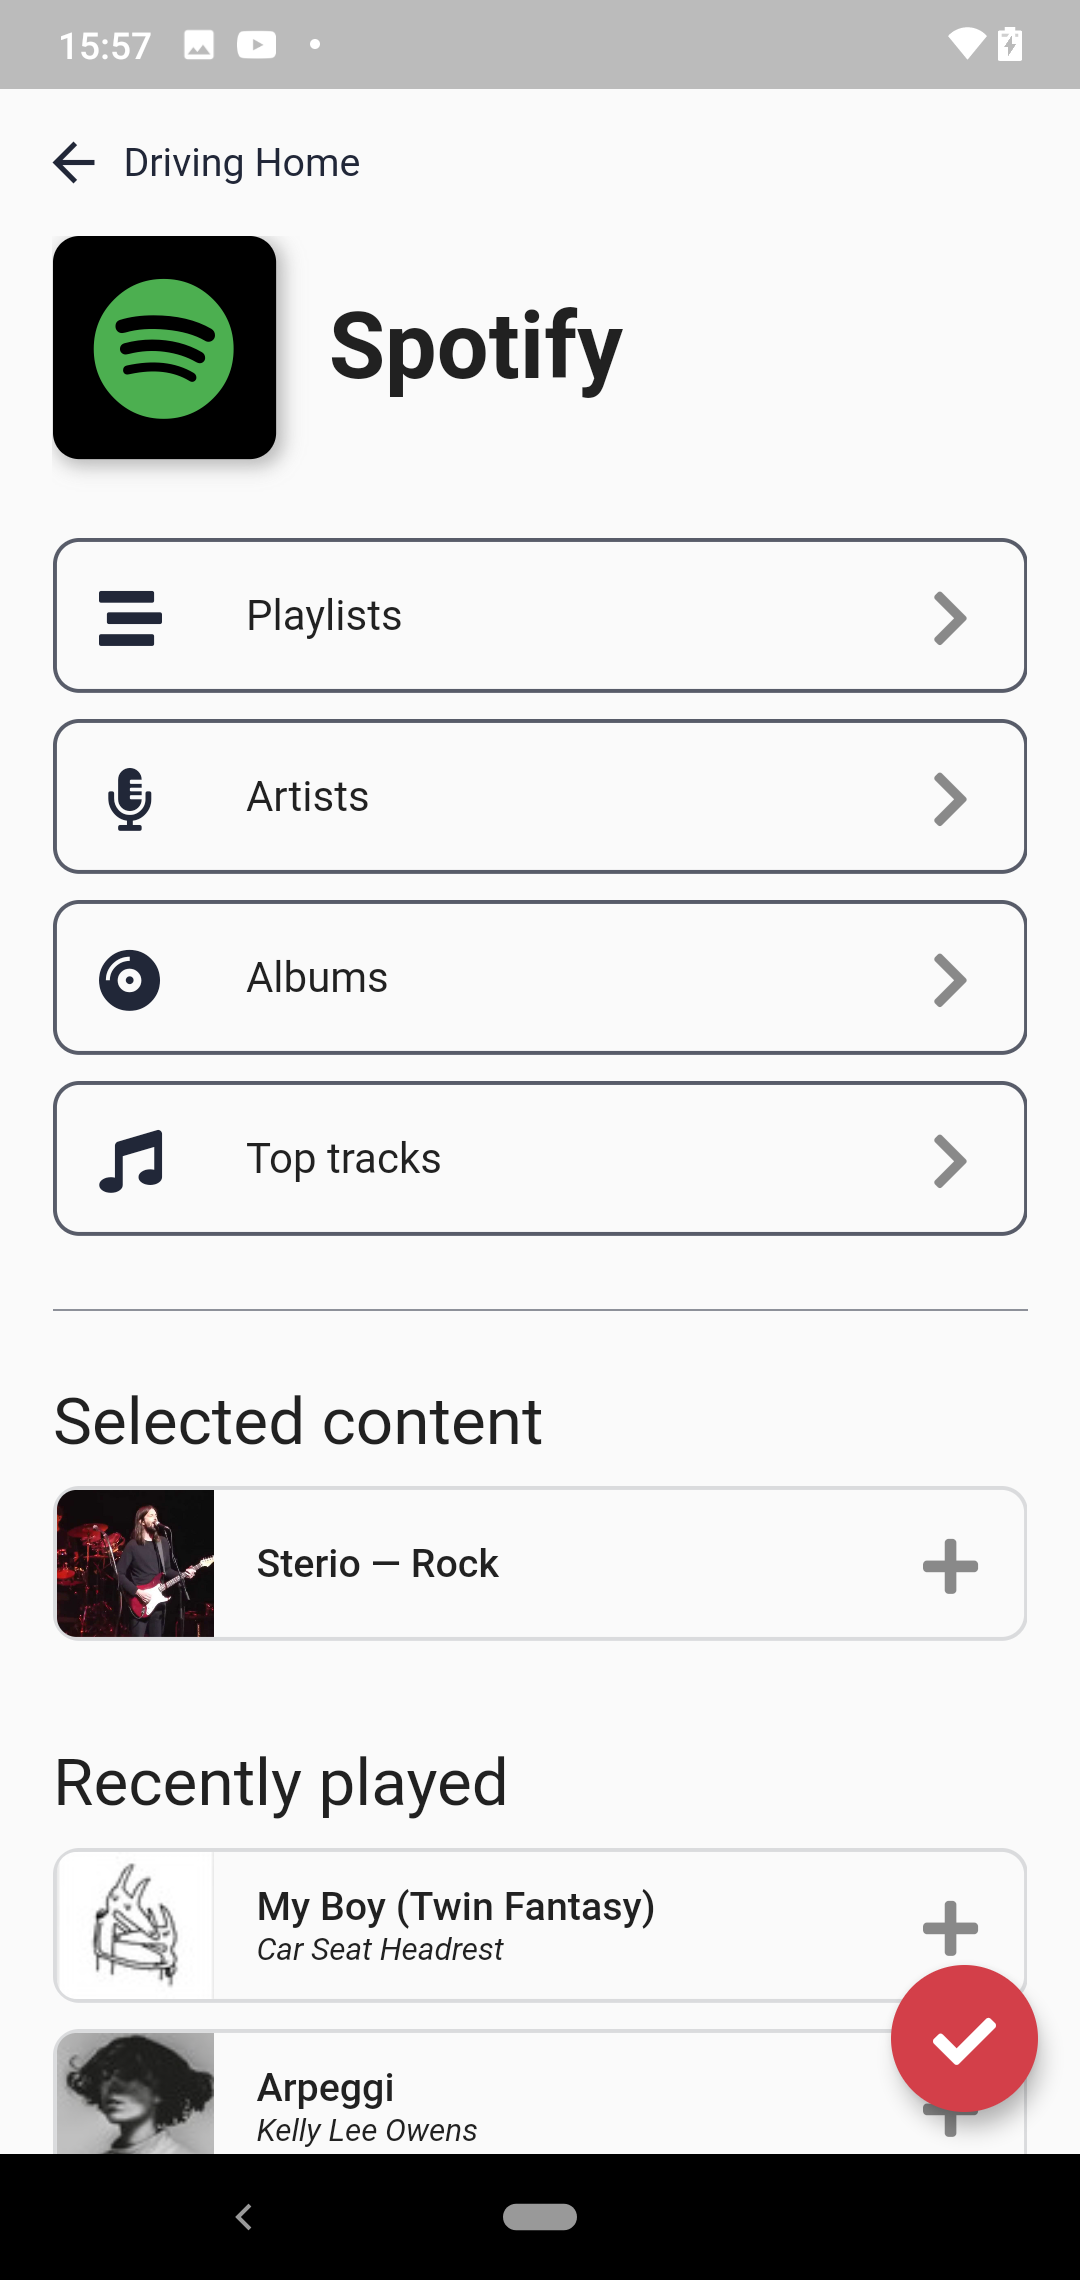
\includegraphics[width=0.29\textwidth]{./Images/screenshots/spotify.png}}} \qquad
	\subfigure[Playlists selection screen]{\label{fig:spotify2}
	\frame{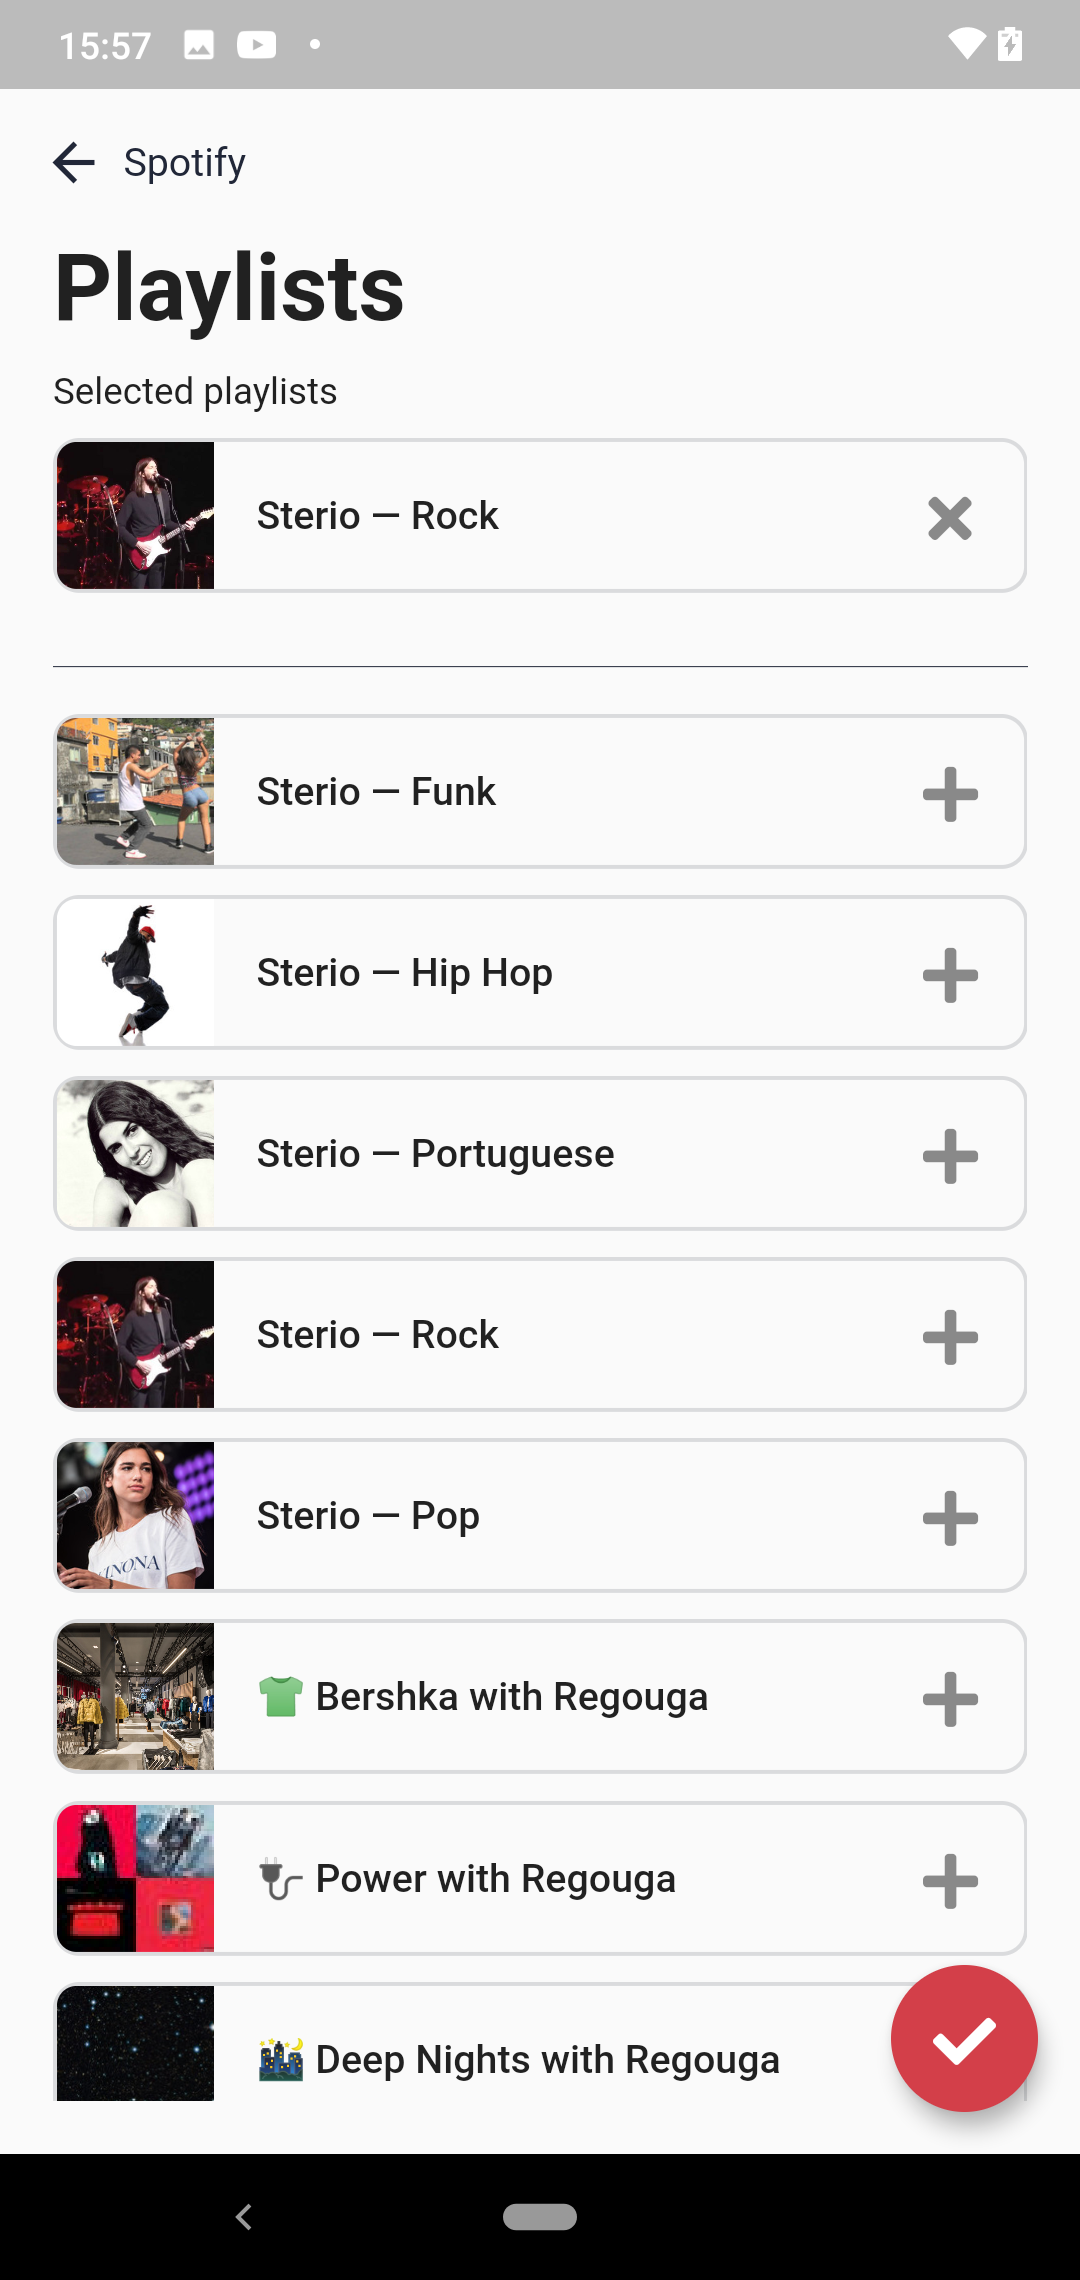
\includegraphics[width=0.29\textwidth]{./Images/screenshots/playlists.png}}} \qquad
	\caption{Spotify block configuration screens}
	\label{fig:spp1}
\end{figure}

Each item (song, album, playlist, artist, or podcast) is represented by a unique \ac{URI}, which are obtained with the resource to the Spotify Web \ac{API} ~\footnote{For more information on the development resources provided by Spotify, visit the \href{https://developer.spotify.com/documentation/web-api/}{Spotify for Developers website}}. The credentials entered by the user (described in Section ~\ref{subsec:lsa}) are used to authenticate and make an API call requesting the desired information. A response JSON file is sent to the backend, where it is processed and, afterward, the information is presented to the user, where they can add the desired content to the station.

\begin{figure}[h]
\centering
\frame{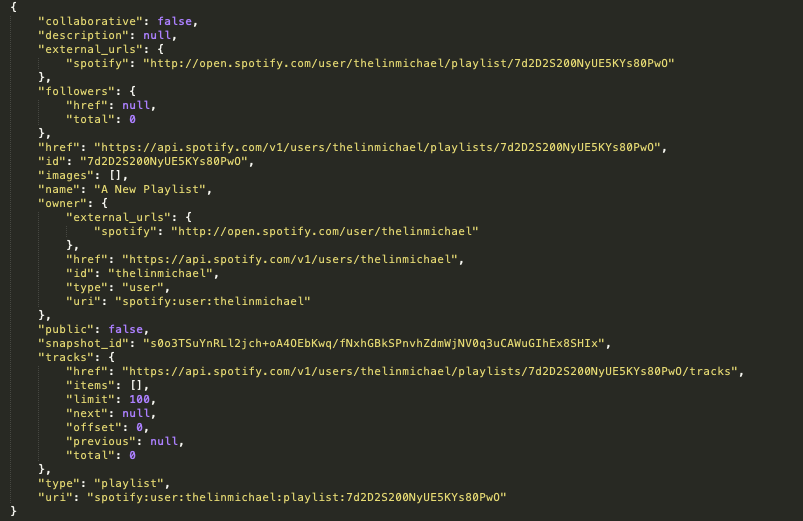
\includegraphics[width=0.8\textwidth]{./Images/code/jsr.png}}
\caption{Response JSON file of a call to the playlist library of Spotify's Web API}
\label{fig:mys}
\end{figure}


The Spotify Web \ac{API} provides several useful features in the context of our project. For instance, it is possible to search the entire Spotify catalog for a specific element, get curated playlists created by Spotify’s editorial team based on popularity, mood, international events, and genres, or even present the best content recommendations based on a variety of terms such as market, seeds (artists, genres, tracks), ranged audio features (danceability, valence, tempo, liveness) and popularity. In the end, this creates a very integrated and personalized experience for the platform's users.

The selected \acp{URI} are linked to the matching station and stored in the database, so that when a user plays a station, Spotify can gather this information and use it to play an individual item. This algorithm — that uses Spotify's Playback \ac{API}, rather than the Web \ac{API} — is further explained in detail in Section ~\ref{subs:playing}.
\newpage

\subsubsection{Weather}

\begin{figure}[htbp]
	\centering
	\subfigure[Main configuration screen]{\label{fig:news1}
	\frame{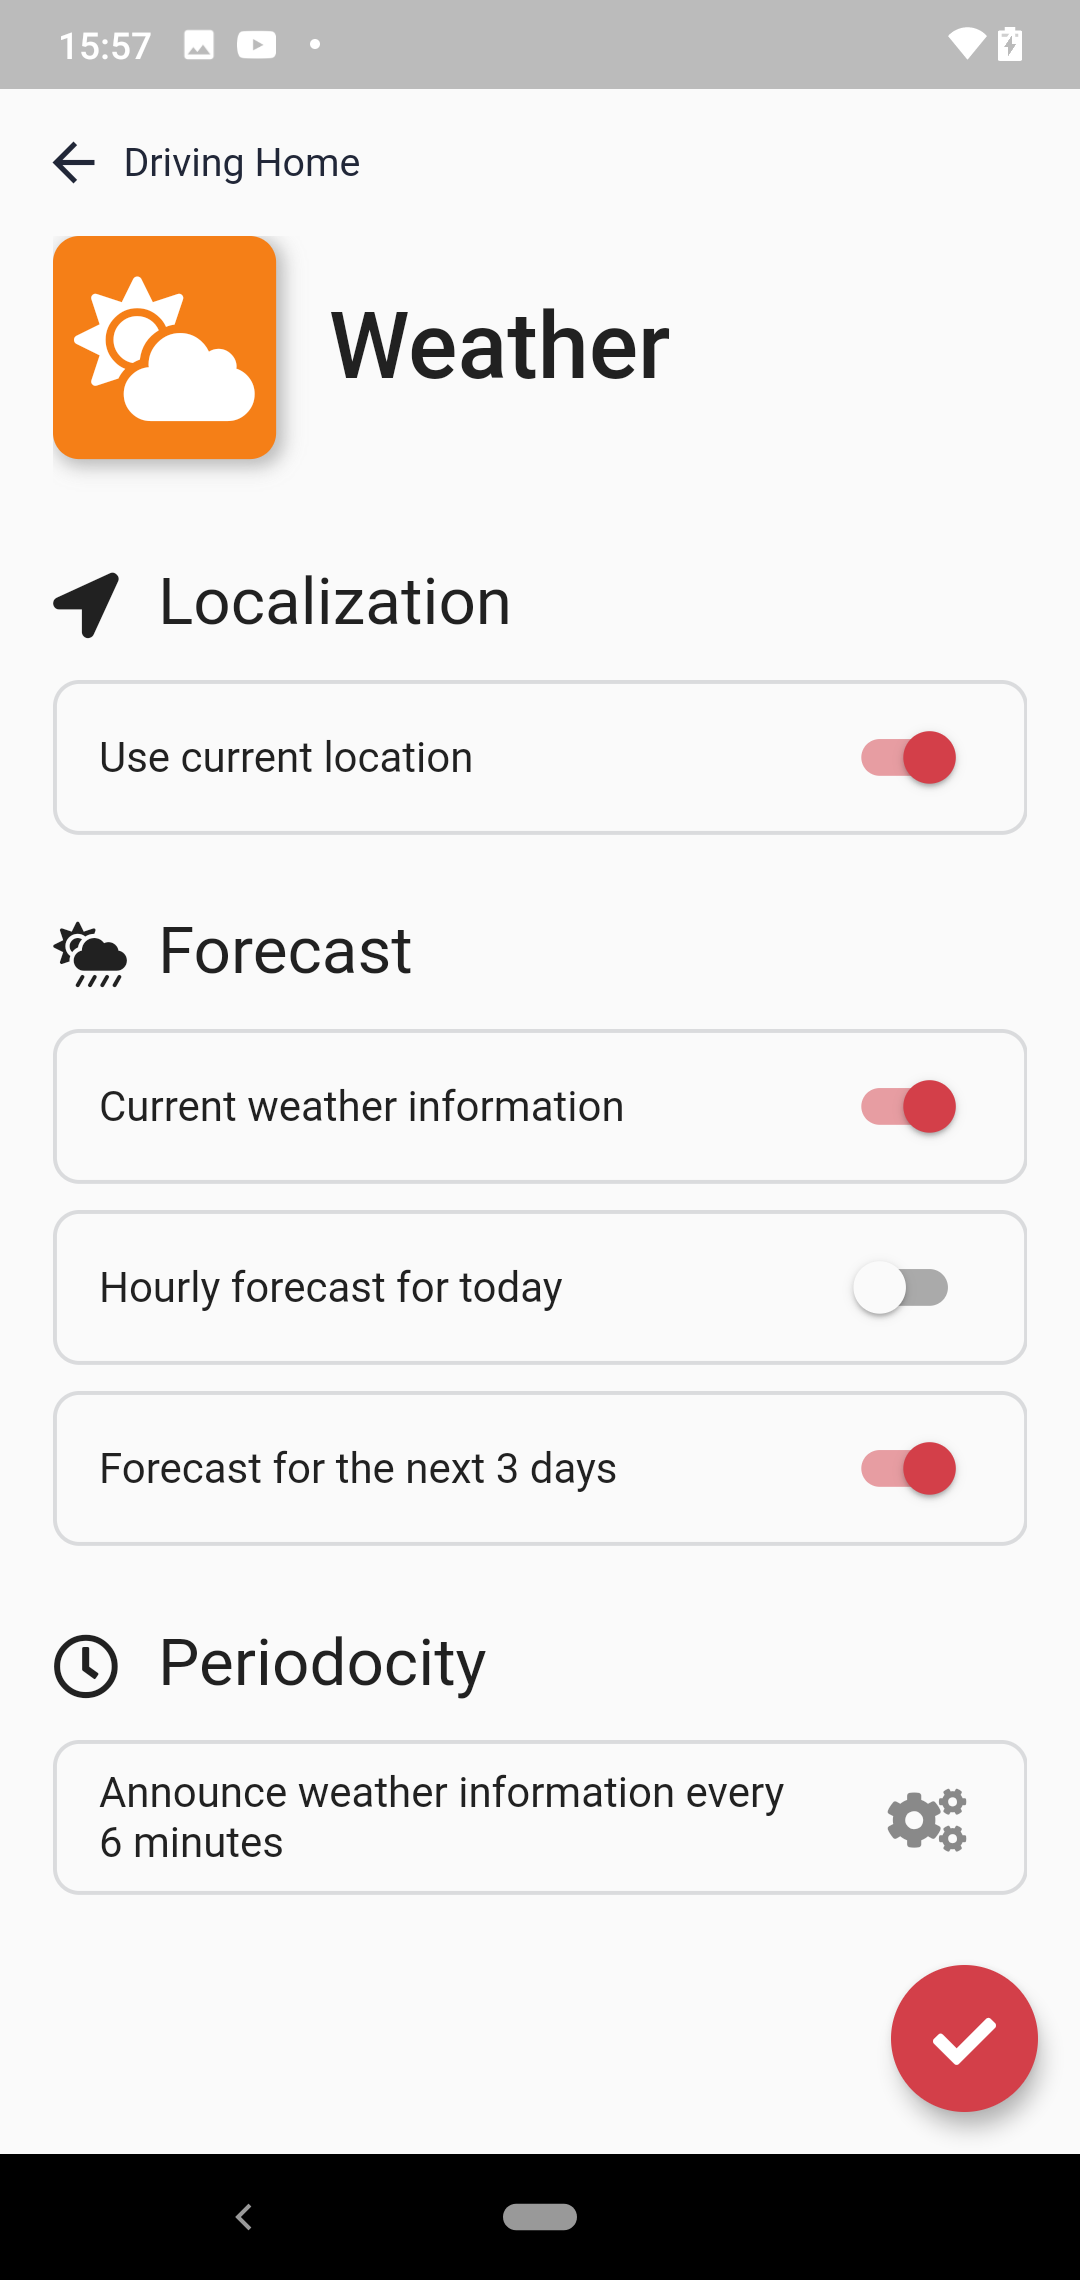
\includegraphics[width=0.29\textwidth]{./Images/screenshots/weather.png}}} \qquad
	\subfigure[Dial selector of weather periodicity]{\label{fig:news2}
	\frame{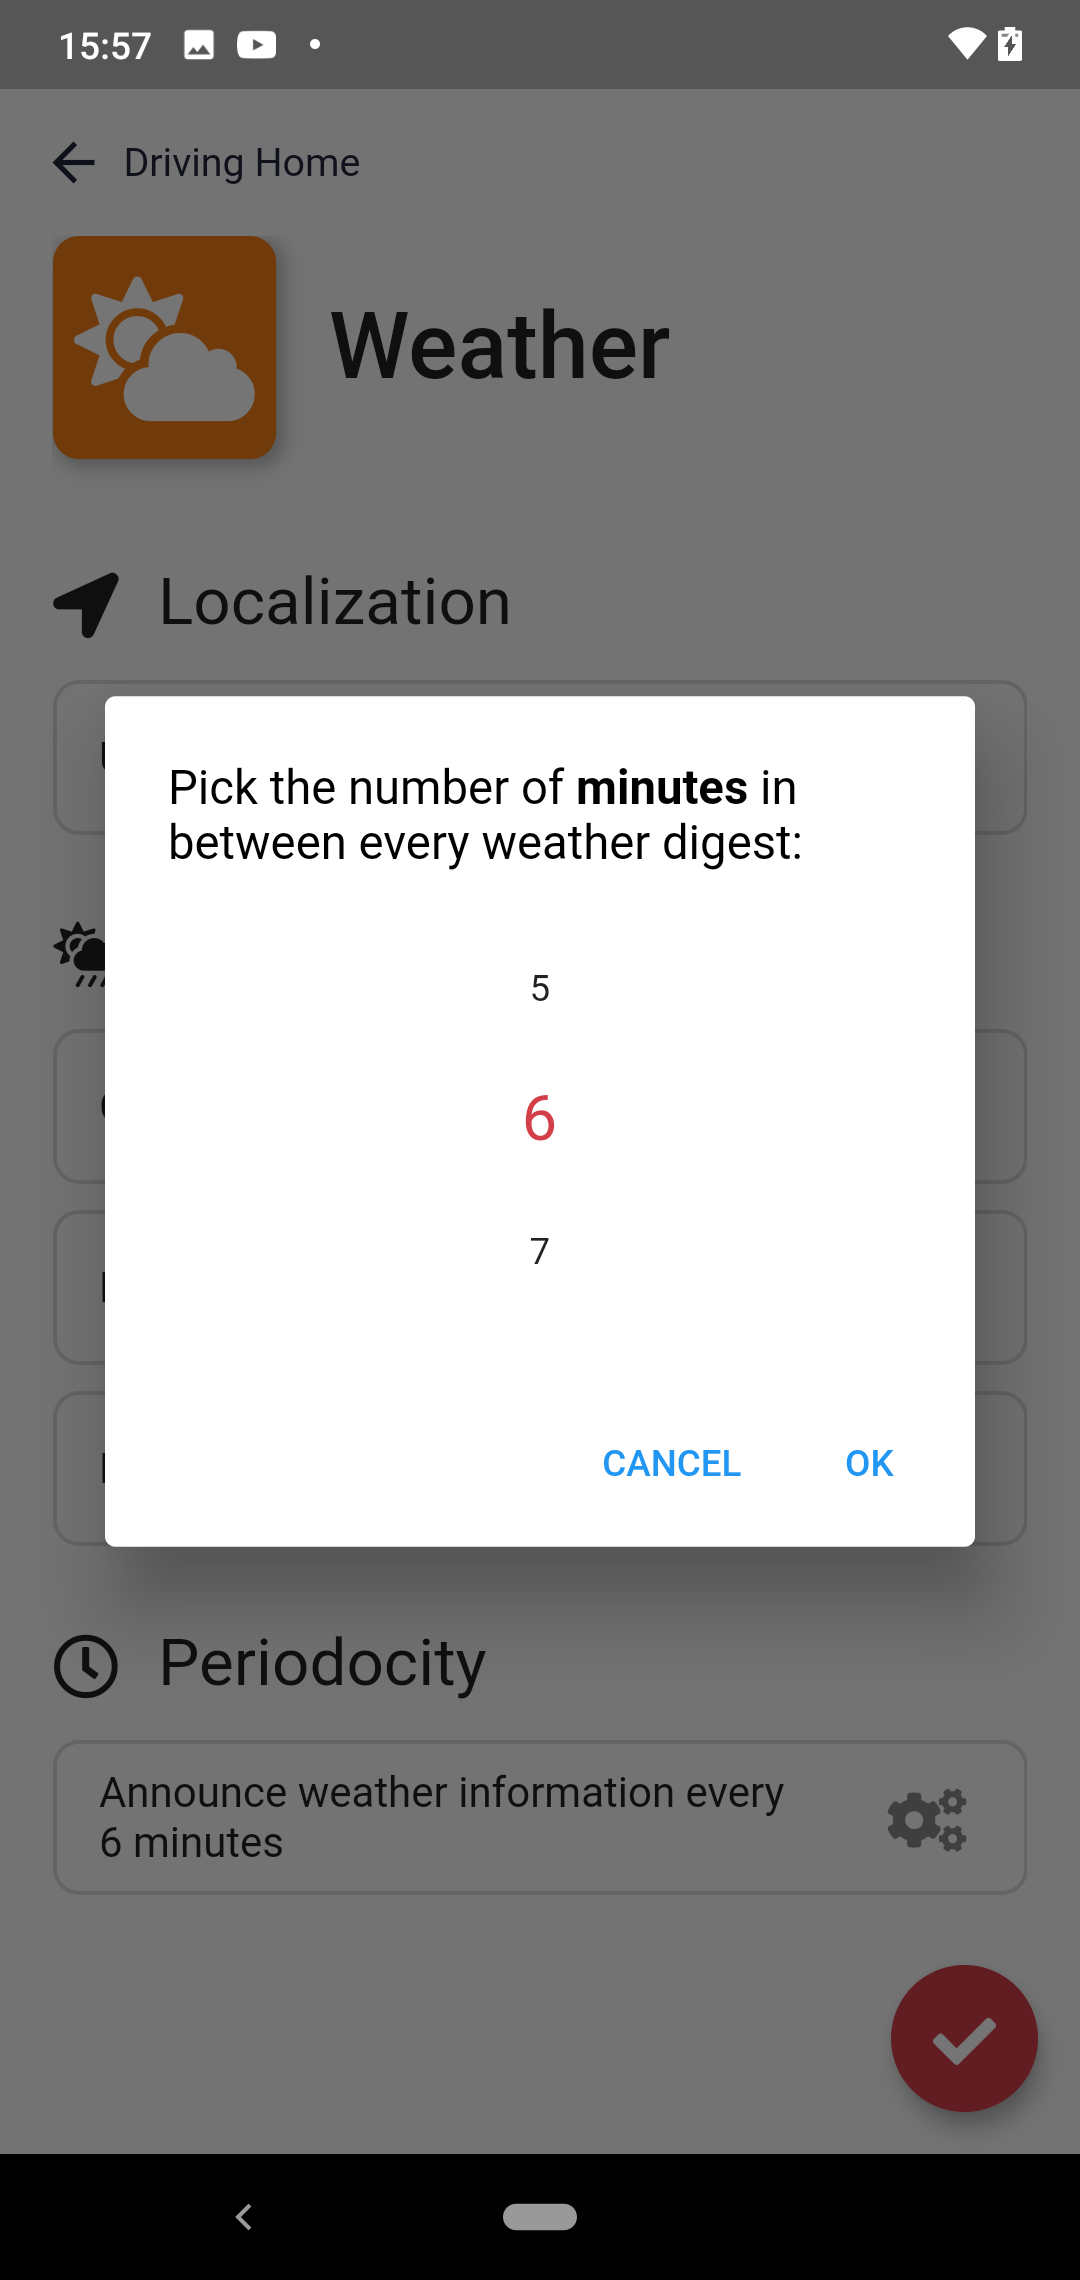
\includegraphics[width=0.29\textwidth]{./Images/screenshots/dial.png}}} \qquad
	\caption{Weather block configuration screens}
	\label{fig:weather}
\end{figure}

The Weather block provides real-time and updated climate information to a given station. Users can choose to listen to the current weather information, hourly forecast for the current day, and/or forecast for the following three days. It is also possible to customize the periodicity of when this information is played in the station, which will change its matching schedule. Finally, users can also set the location from which they want to receive weather information — by default, this is attributed to the user's current location. These settings set by the user are stored in the database.

To gather meteorology information, we rely on the OpenWeather Map \ac{API} ~\footnote{For more information on used API, visit the \href{https://openweathermap.org/api}{OpenWeather API website.}}, which provides the required information reliably and effortlessly. A 'GET' request is made to the \ac{API}, which response is a JSON file containing all the necessary information. 

\newpage
\subsubsection{News}

The News block provides a digest of the top headlines to a given station. Users can select the categories of news they wish to listen to, the number of headlines, and the periodicity of the digest. It is also possible to select a specific keyword to fetch news from (e.g. "COVID-19"), or even select the sources from where the headlines are retrieved. These settings set by the user are also stored in the database.

We used the News \ac{API} to fetch this information, which delivers breaking news headlines, and allows the search for articles from news sources and blogs all over the web~\footnote{For more information on used API, visit the \href{https://newsapi.org/}{News API website.}}. Just like on the Weather block, a 'GET' request is made to the \ac{API}, which response is a JSON file containing all the requested information by the user.

\begin{figure}[htbp]
	\centering
	\subfigure[News categories selection]{\label{fig:news1}
	\frame{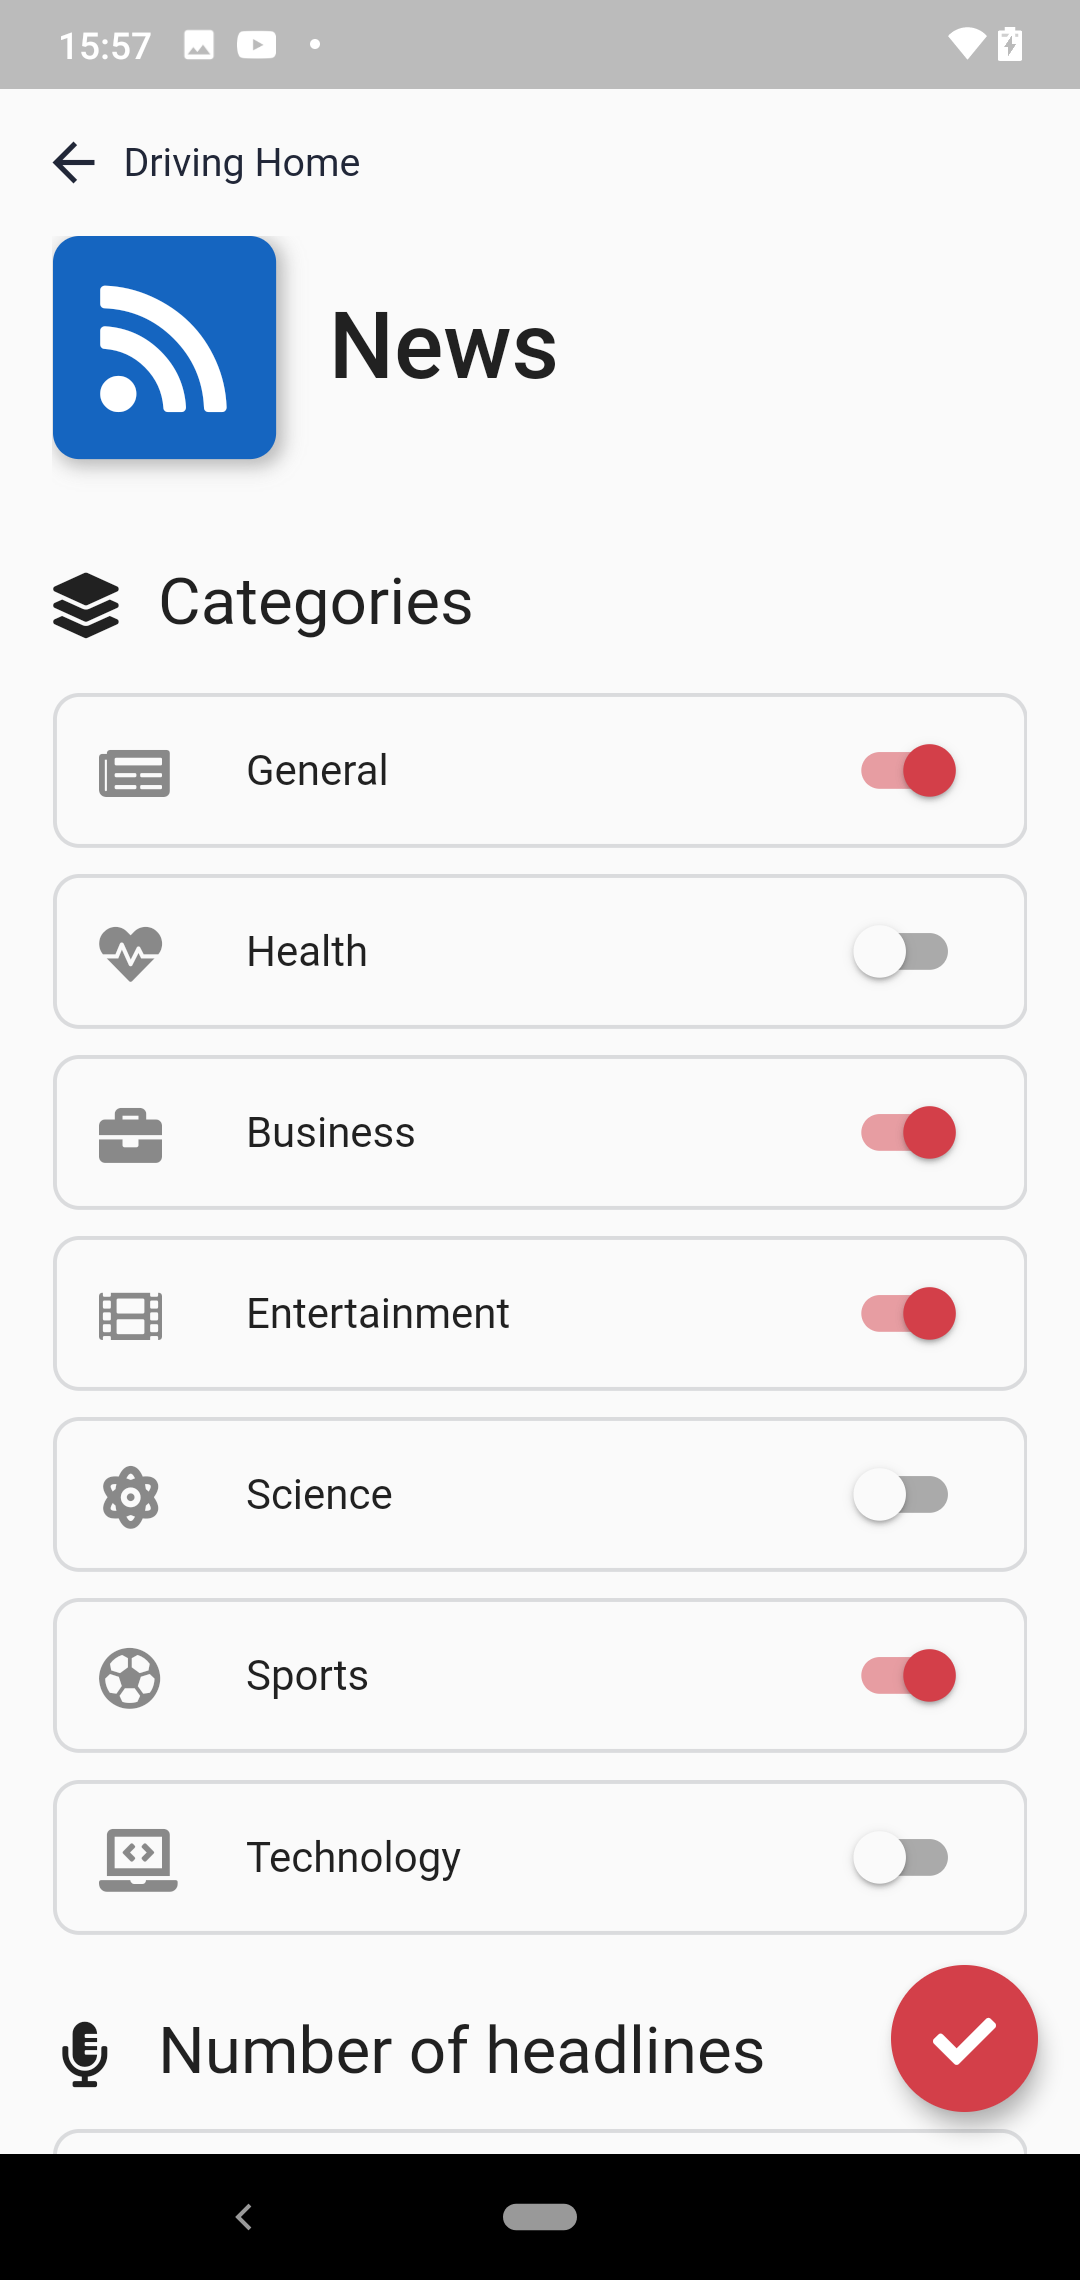
\includegraphics[width=0.29\textwidth]{./Images/screenshots/news1.png}}} \qquad
	\subfigure[Number of headlines and periodocity]{\label{fig:news2}
	\frame{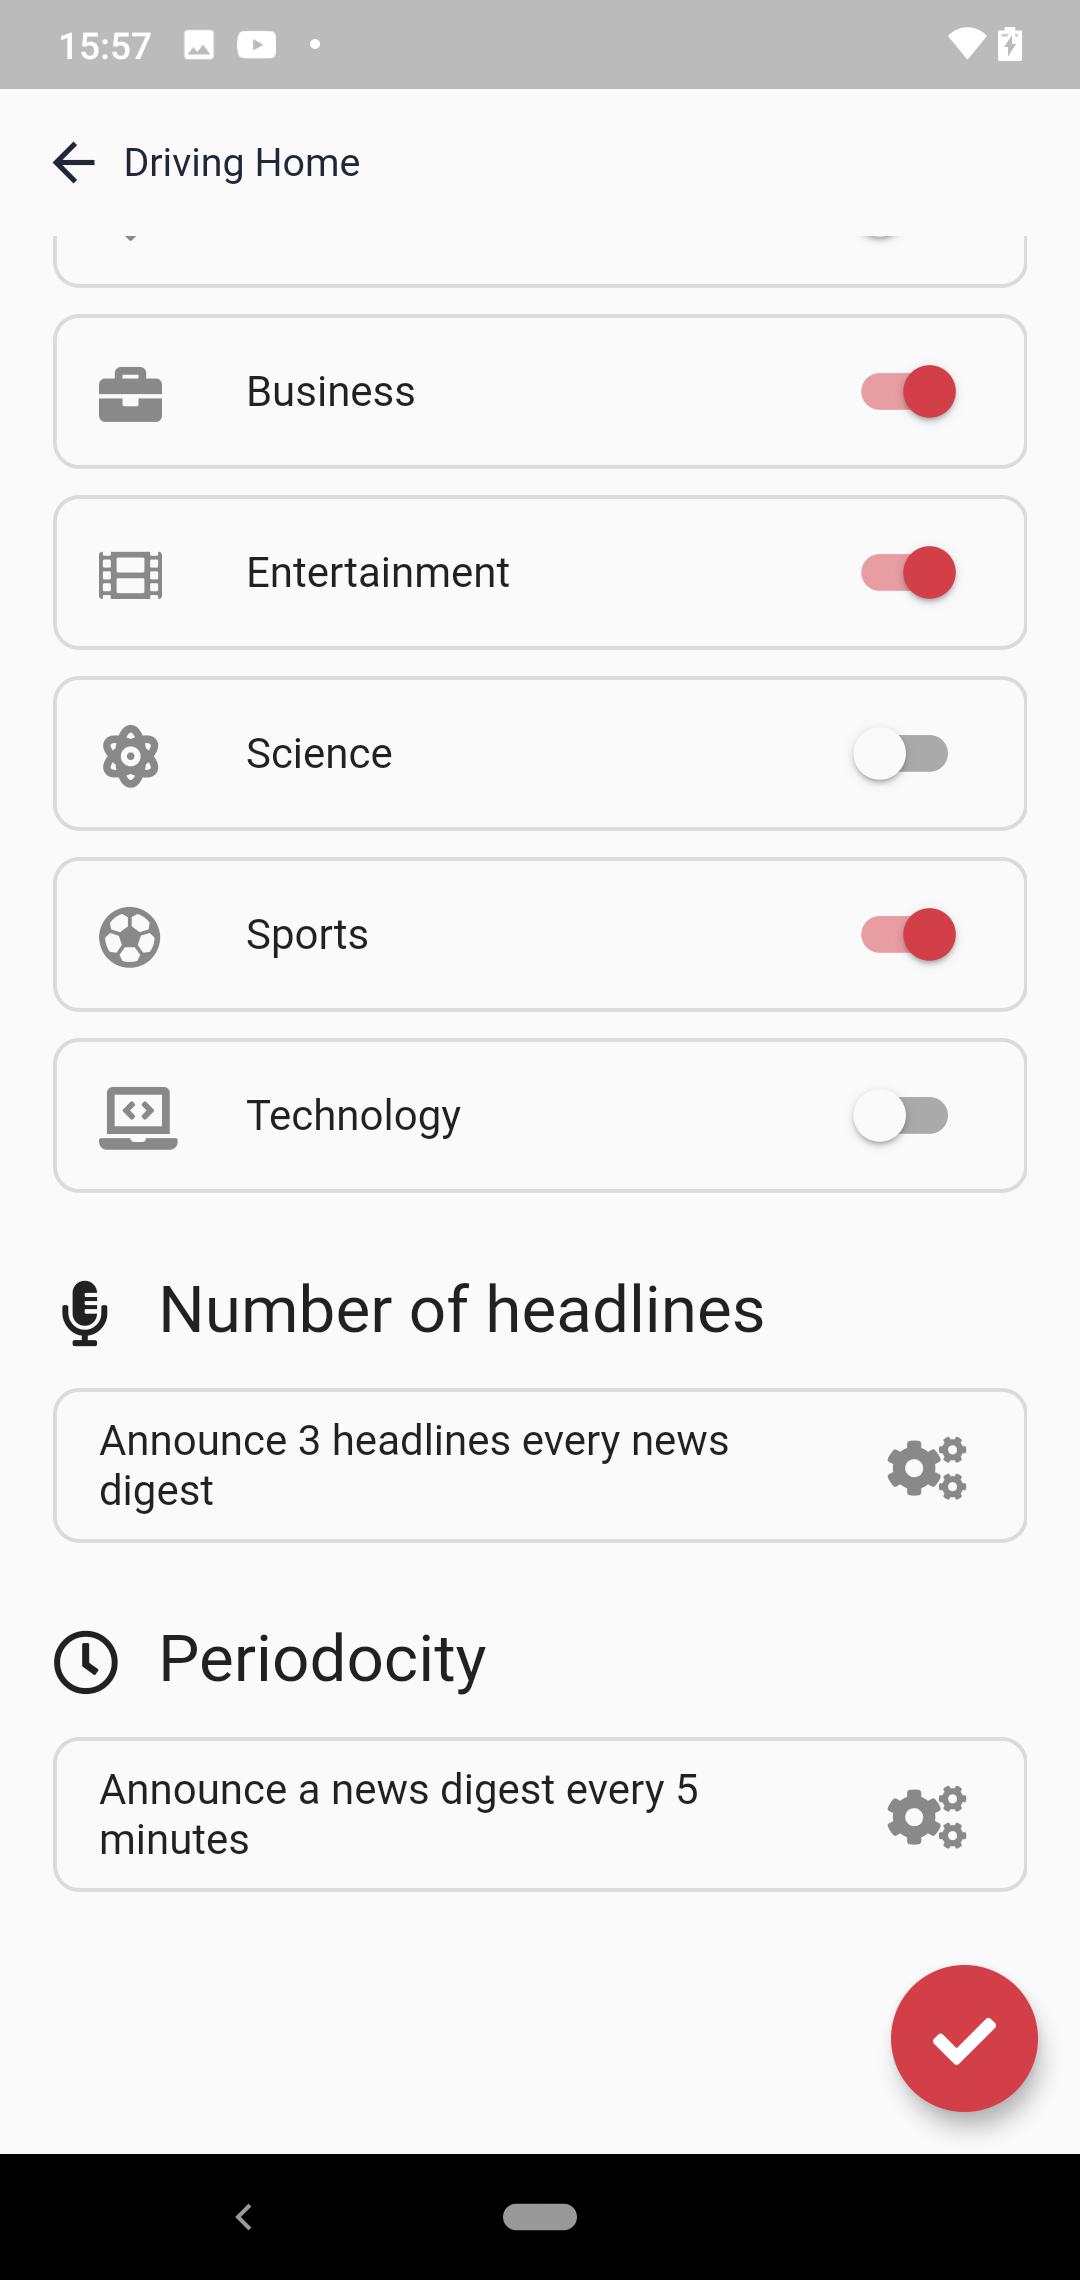
\includegraphics[width=0.29\textwidth]{./Images/screenshots/news2.png}}} \qquad
	\caption{News block configuration screens}
	\label{fig:mfp1}
\end{figure}


When the News block is played in the station, each headline is synthesized and announced by the text-to-speech software, just like any other block containing readable information. To each headline, a small, descriptive block of text is added to provide more context on the news. Then, an audio separator is played, so that the user knows when the announcement of the next headline begun.

The headlines are obtained based on the country and language selected by the user in the signup process of the platform. Nevertheless, the user has full control over this matter and can choose to obtain news headlines from a variety of search terms, topics, countries, languages, and categories.



\begin{figure}[h]
\centering
\frame{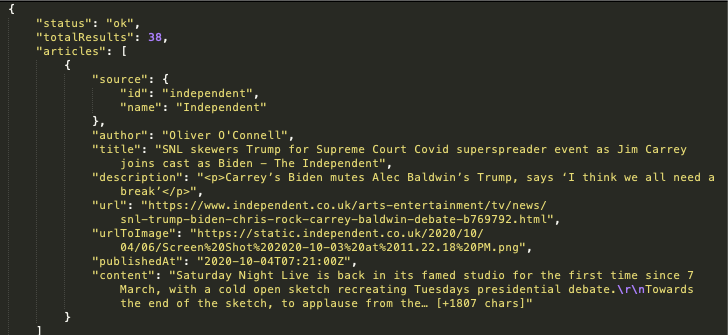
\includegraphics[width=0.8\textwidth]{./Images/code/news.png}}
\caption{Response JSON file of a call to the News API}
\label{fig:mys}
\end{figure}

\newpage
\subsection{Playing a Station}
~\label{subs:playing}

When the station is fully customized to the user's taste, it is then possible to play it. To do so, the user simply needs to tap the 'Play' button, located either at the station information screen or at the preview card displayed on the 'My Stations' screen. 

After tapping the 'Play' button, a modal, represented in Figure ~\ref{fig:play1} is shown to the user, which acts as a 'loading' screen while the backend of the platform performs the necessary tasks to allow the playing of the station. To give a radio-like experience, it is played an audio track that mimics the sounds of tuning into a traditional terrestrial radio station, which automatically stops when all loading processes are complete. 

\begin{figure}[htbp]
	\centering
	\subfigure[Loading ("tuning") screen]{\label{fig:play1}
	\frame{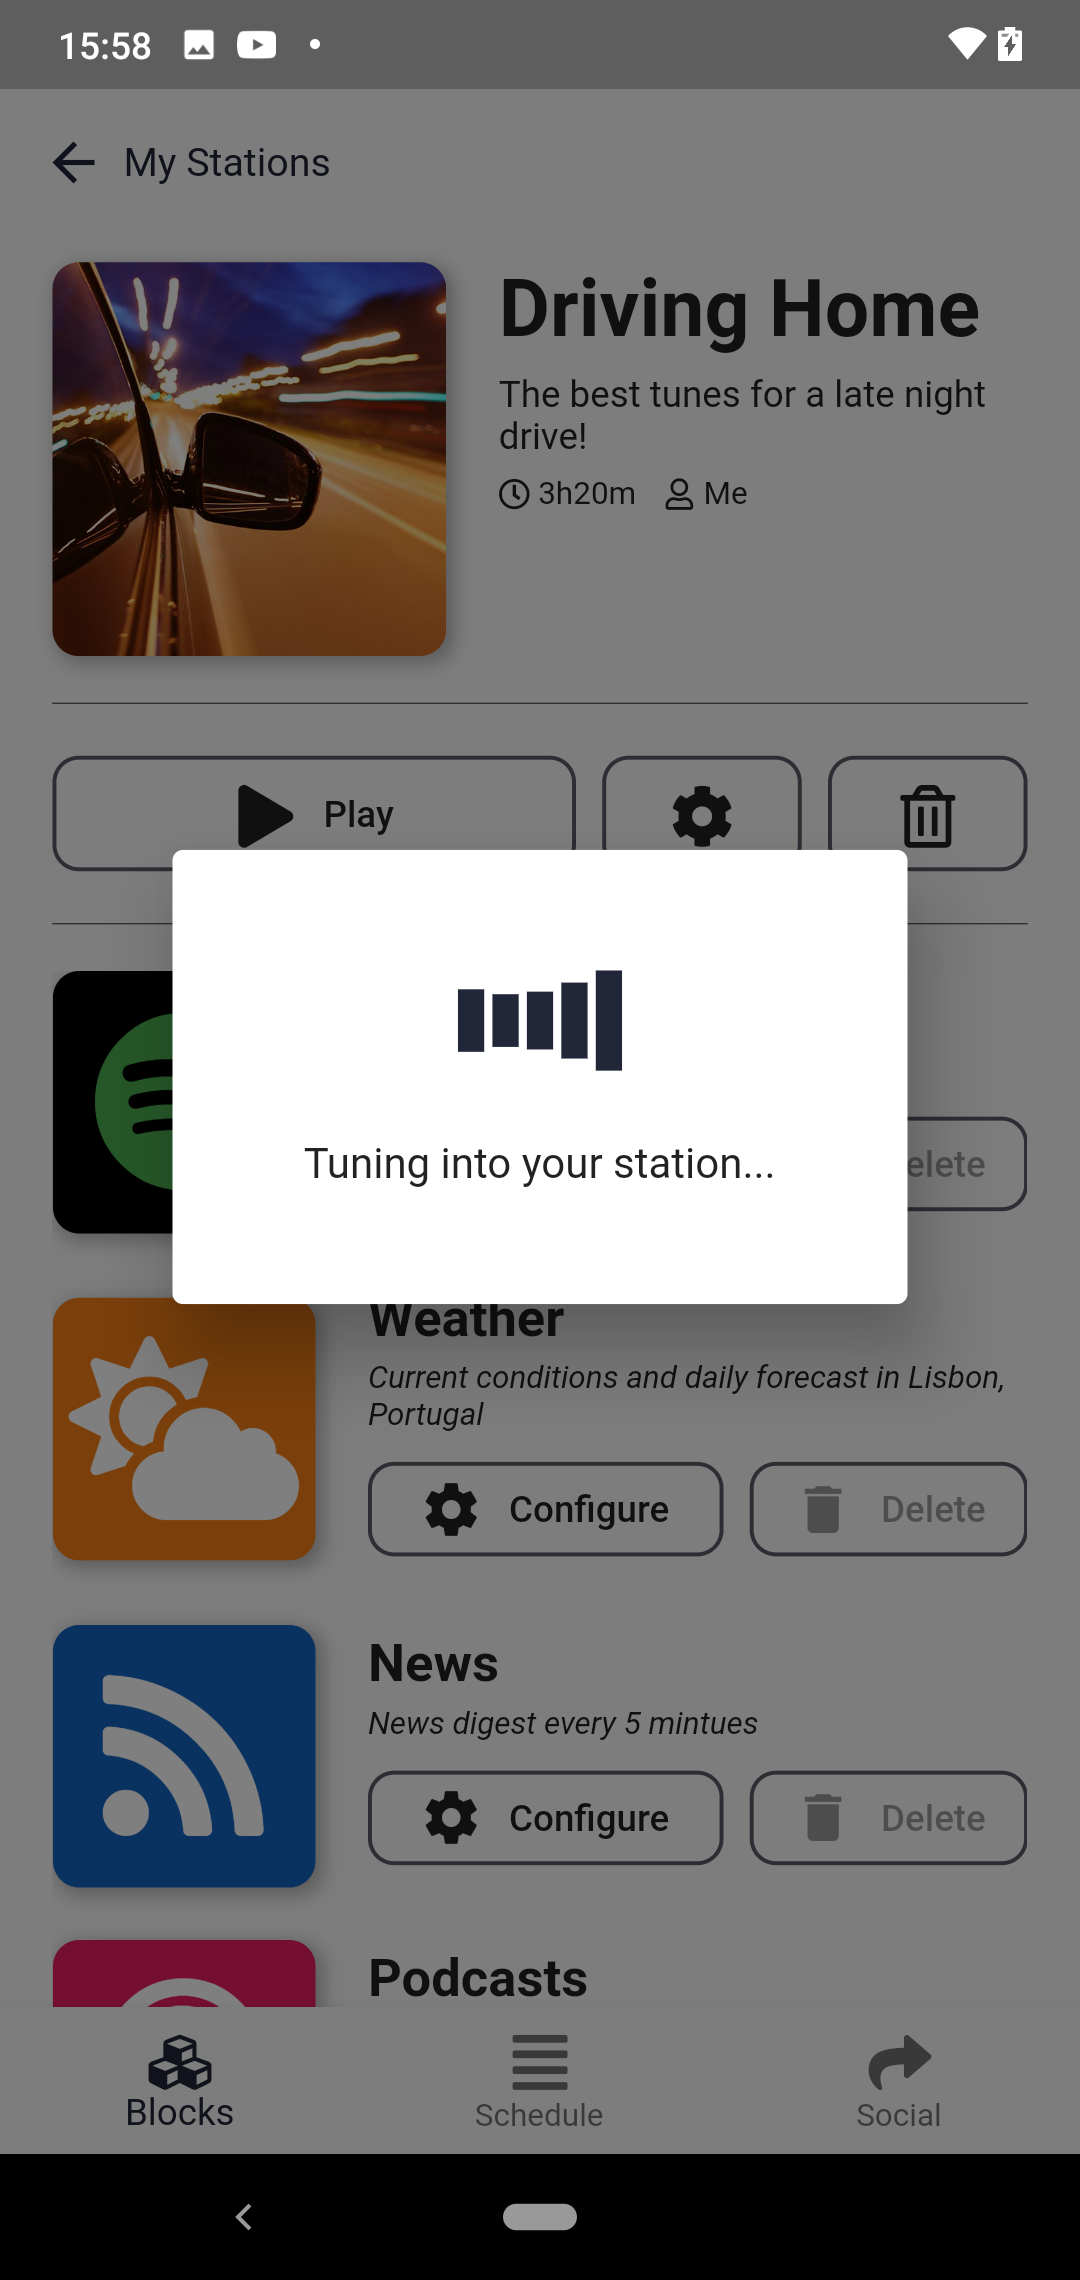
\includegraphics[width=0.29\textwidth]{./Images/screenshots/play1.png}}} \qquad
	\subfigure["Now Playing" controller bottom bar]{\label{fig:play2}
	\frame{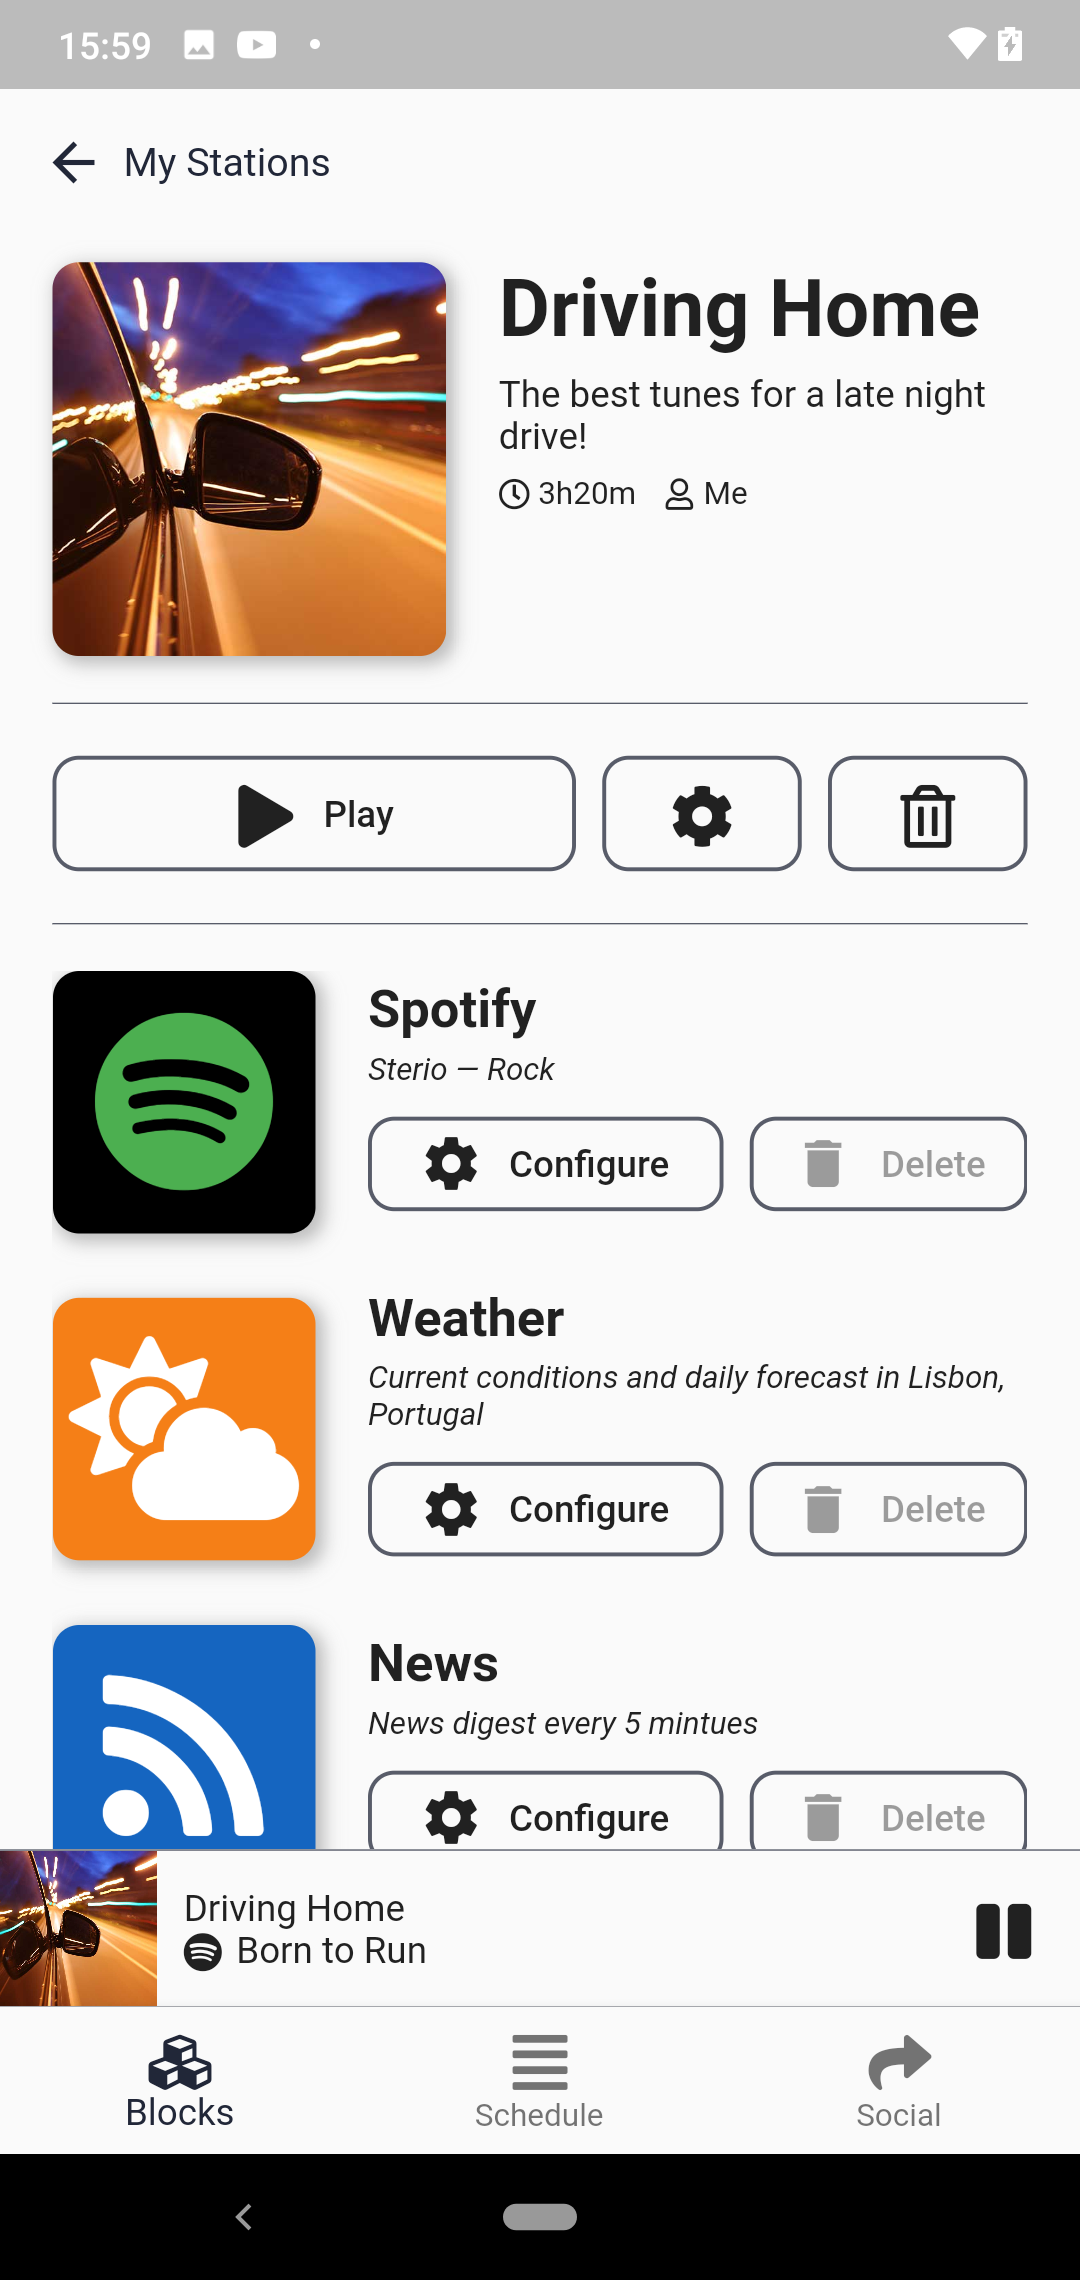
\includegraphics[width=0.29\textwidth]{./Images/screenshots/play2.png}}} \qquad
	\caption{Playing a station}
	\label{fig:mfp1}
\end{figure}

\newpage

Finally, the station starts playing, and a 'Now Playing' controller bar, shown in Figure ~\ref{fig:play2}, is displayed. This bar provides quick and easy information to the user regarding what's currently playing, as well as a 'Play/Pause' button to stop playback when needed. If the user taps this bar, the 'Now Playing' screen, showcased in Figure ~\ref{fig:npslol} is shown, which provides more playback controls and information regarding the currently playing station, including the content that will be played next in the schedule.

\begin{figure}[htbp]
	\centering
	\subfigure[Now playing screen]{\label{fig:np1}
	\frame{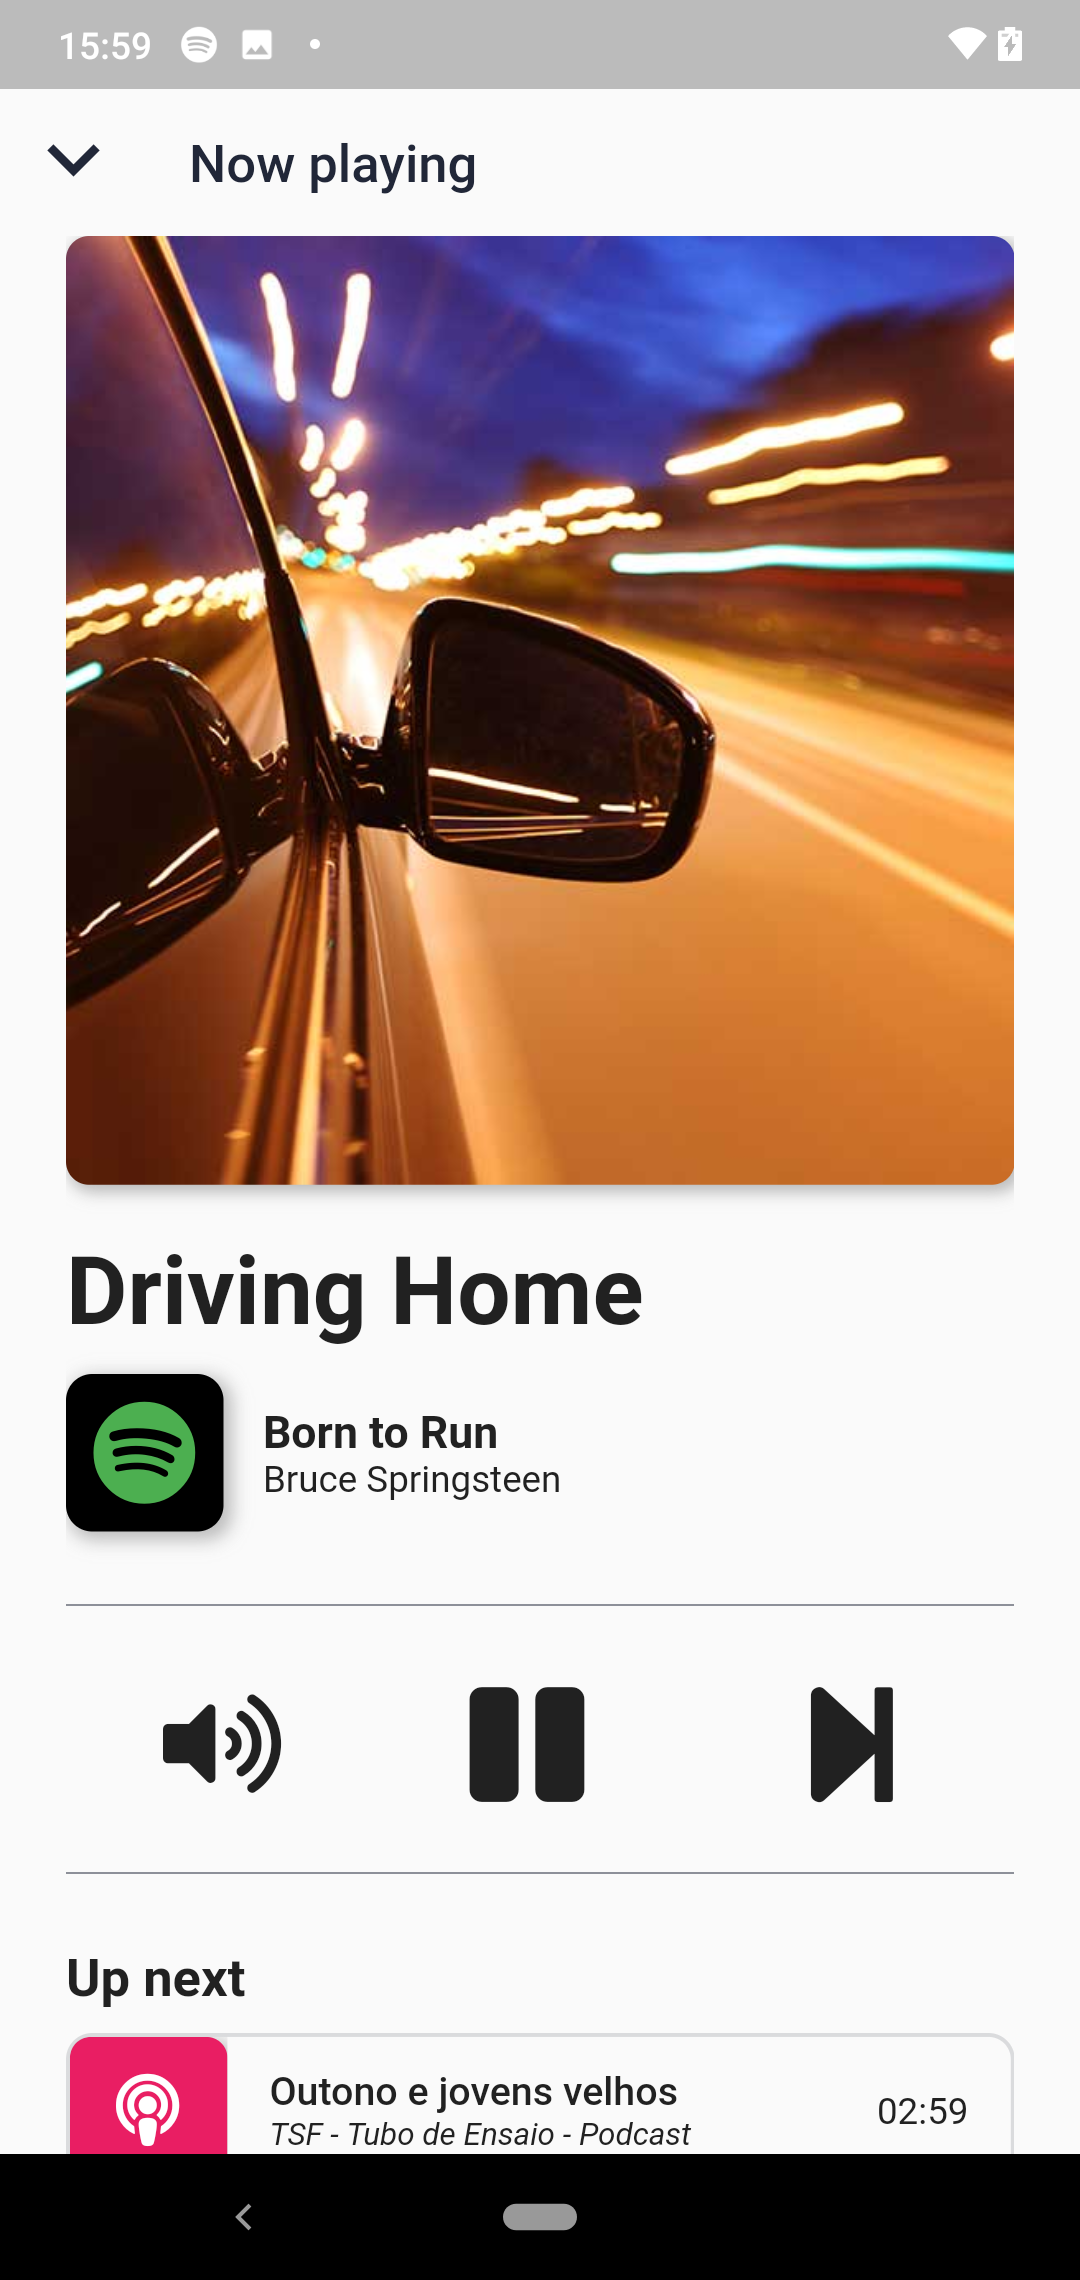
\includegraphics[width=0.29\textwidth]{./Images/screenshots/np1.png}}} \qquad
	\subfigure[Up next content]{\label{fig:np2}
	\frame{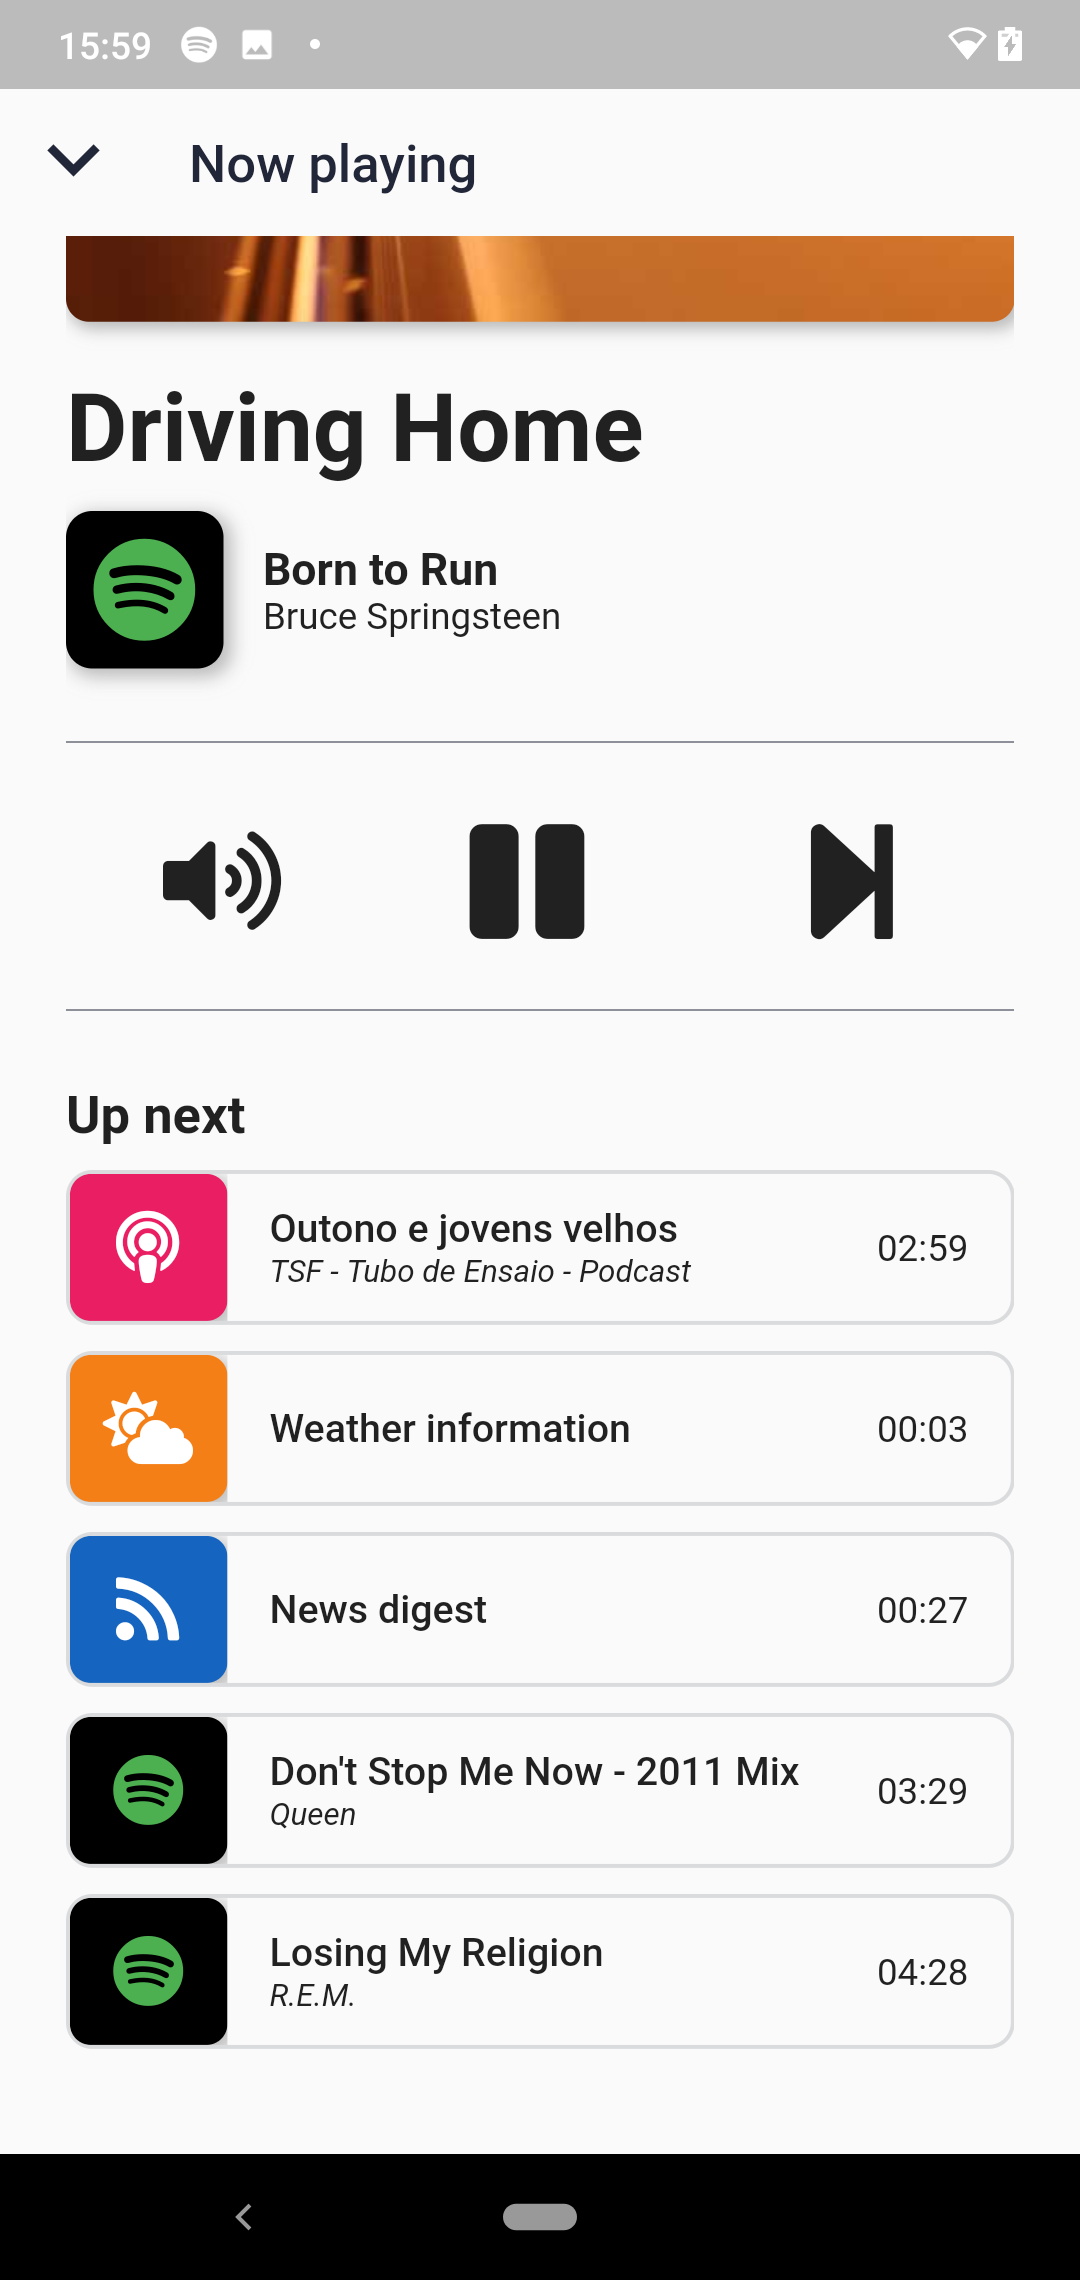
\includegraphics[width=0.29\textwidth]{./Images/screenshots/np2.png}}} \qquad
	\caption{"Now Playing" screen}
	\label{fig:npslol}
\end{figure}

\begin{figure}[h]
\centering
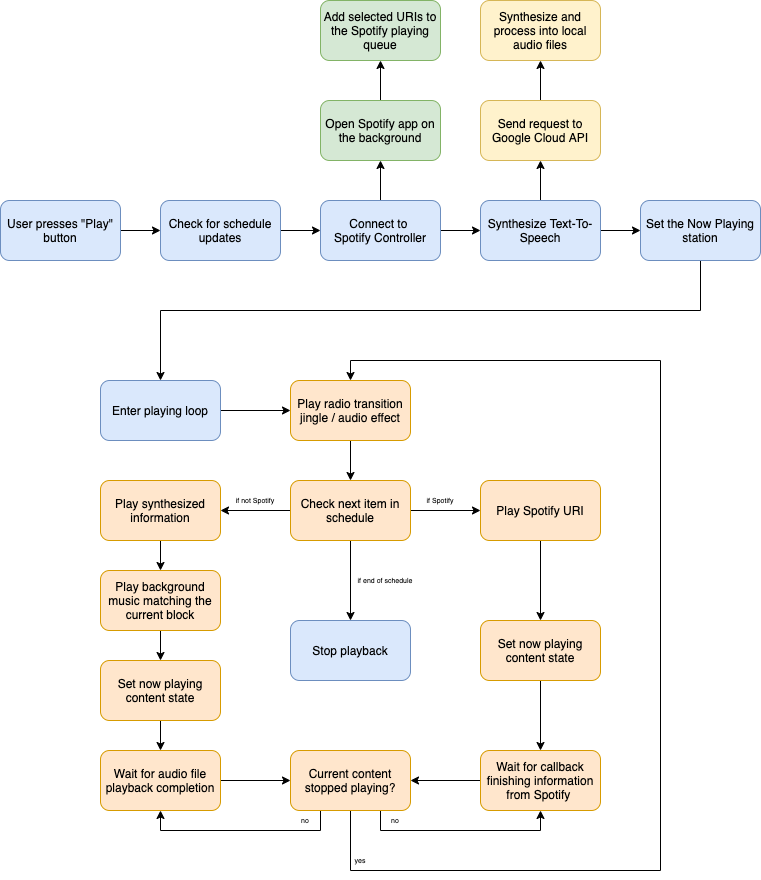
\includegraphics[width=0.8\textwidth]{./Images/code/alg.png}
\caption{Algorithm for playing a given station}
\label{fig:alg}
\end{figure}


To play the station, a 5-step algorithm is performed before entering the main playing loop. This algorithm is represented in Figure ~\ref{fig:alg}.

After pressing the play button, the first step of the algorithm is to check if the user has changed the configurations of any of the selected blocks, or if the schedule playing order has been modified. If it is the case, the algorithm updates and processes the schedule so that it is performed on the most recent configurations of the station.

Following this process, the platform will connect to the Spotify Controller, which is a dedicated component of the code that connects to the Spotify Playback \ac{API}. As mentioned in Section ~\ref{sub:spotify}, this is a different \ac{API} library from the one used to select the desired content from the music streaming service.

To control a user's Spotify playback, the \ac{API} requires that the Spotify application is installed on the user's device and that it is opened in the background, so that it can receive requests. This is a limitation set by the Spotify \ac{API} that we can't bypass. After the connection to the Spotify Controller is successful, then all the selected content (\acp{URI}) is added to the user's Spotify listening queue.

After the Spotify connection is handled, all the information from the remaining station's blocks is fetched, so that it is as updated and real-time as possible. The responses are then processed into a natural spoken text, which is then sent as a 'GET' request to the Google Cloud Text-to-Speech API~\footnote{For more information on used API for the text-to-speech synthesizer, visit the \href{https://cloud.google.com/text-to-speech/docs}{Google Cloud Text-to-Speech API website.}}. The API responds with a set of encoded information containing the synthesized sound bytes, which are locally converted into audio files. These audio files are then stored in the cache of the platform which, after playing the station, are discarded to save storage space.

Then, if Spotify successfully connected to the platform, and if all the requested information from the blocks is successfully synthesized into text-to-speech audio files, the last step before entering the main playing loop is to set the 'Now Playing' station as the current 'state' of the platform. This allows the access and control of the currently playing station throughout the interface, as shown in Figures ~\ref{fig:play2} and ~\ref{fig:npslol}.

Finally, the station enters its main playing loop. Every station begins with a radio transition jingle or audio effect that serves as a separator between content, mimicking a traditional terrestrial radio station, and granting a more cohesive and integrated experience to the user. This transition is naturally inserted between music tracks or other content to allow continued attention in the periphery. Transitions can also be turned off if the user wants a more synthetic listening experience.

Following this introductory audio effect, the algorithm checks whether the next item of the schedule is a Spotify \ac{URI} or not. If it is, it plays it by simply calling a 'play' function provided by the Spotify Controller, and sets the now playing state of the application. Then, the algorithm checks if the current Spotify content has finished playing, and, if so, it plays an audio transition and another iteration of the loop is processed.

The most difficult challenge we faced while coding this algorithm was the process of determining whether the Spotify content has finished playing or not. The Spotify Playback \ac{API} does not provide an easy way of accessing this information, allowing only the access of a limited set of playback information, such as the current position of a content's playback. To bypass this limitation, we crafted a sub-algorithm that checks second by second this information, and when the current position of a content's playback matches the total length of such content, an alert is sent to indicate that the content has finished playing. This approach adds complexity in terms of performance and resource usage, but it was the only way we found to bypass this limitation set by the Spotify Playback \ac{API}.

Conversely, if the next item on the schedule is not a Spotify \ac{URI}, then the algorithm picks up the matching synthesized audio file and plays it. At the same time, matching background music is added while the text-to-speech audio file is played, so that the user creates more empathy while listening to the information. The now playing state of the application is also set, and if the algorithm checks if the current content has finished playing, it plays an audio transition, and another iteration of the loop is processed. As we're processing local files, we didn't face the same issues in determining if the currently playing content has finished playing, unlike we had with Spotify content playback.

When the station finishes playing its matching schedule, the playback is stopped and all the local cached files are deleted. Nevertheless, the user can choose to loop or repeat the station, allowing a non-stop playback of content.


% If Printing on DOUBLE SIDED pages, the second page should be white.
% Otherwise, comment the following command:
\cleardoublepage
%
%Chapter 6
% #############################################################################
% This is Chapter 6
% !TEX root = ../main.tex
% #############################################################################
% Change the Name of the Chapter i the following line
\fancychapter{Evaluation}
% The following line allows to ref this chapter
\label{chap:evaluation}

After completing the last cycle of development, a set of users tested the Sterio system, in order to gather quantitative and qualitative usability metrics to assure that our platform meets both users’ needs and our set goals. We start by presenting the methodology used, followed by the description of the tasks defined for the test sessions, justifying, for each, what we want to conclude by asking users to do it. We finally present the analysis of the test results and the workload estimated for the prototype, as well as the conclusions that we were able to get from the results.


% #############################################################################
\section{Methodology}

When a final functional prototype of the platform with a working set of features was completed, a group of 26 potential users tested the system. This set of users were of distinct ages, occupations, socio-economical backgrounds, and audio media consuming habits. From these users, 21 haven't participated in either of the previously-mentioned user research (described in Chapter ~\ref{chap:userresearch}) and speed dating activities (examined in Chapter ~\ref{sec:speeddating}), while the remaining 5 have participated in these ventures.

This evaluation was conducted to assess the success of the final prototype and to check that a standard was upheld, which is a process known as summative evaluation. ~\cite{Preece2015, Courage2005} The same list of tasks and protocols were presented to each user, and their performance was evaluated mainly through qualitative measures, as we want to deeply understand the type of experience that is created while users indulge in the platform, as well as insights, findings, and anecdotes about the experience of the user.

To help us steer the session, and to keep all gatherings as cohesive and alike as possible, the first step was to write a protocol guide, shown in Appendix CENAS. All sessions were conducted in a physical location, where several measures were taken to comply with health and safety guidelines as a response to the COVID-19 pandemic. For instance, the researcher and the user were seated at least 2 meters apart from each other, complying with the social distancing rules. All surfaces — including the provided smartphone on where the prototype was tested — were disinfected before and after the session. Users were required to utilize hand sanitizer when entering and leaving the room and were also asked to bring their smartphone so that they could fill out the necessary survey forms. 

We planned each testing session to be divided into 3 distinct segments, which we will describe in the following subsections.

\subsection{Introduction, Informed Consent Form, and Initial Survey}

After the user's arrival to the testing room, the facilitator invited them to sit in a comfortable way. In front of them, three items were displayed: a smartphone with the loaded Sterio system; a sheet containing a set of QR codes that redirects users to the necessary survey forms; and a helping sheet that contains extra information regarding the tasks.

In order to contextualize each user on what the purposes of the testing were, an introduction was read by the research. Then, users were asked to carefully read and sign an informed consent form (presented in Appendix CENAS. Finally, by presenting them an initial survey (showcased in Appendix CENAS), we collected demographic information and other relevant details of the user, such as if they had any visual or hearing conditions, as well as their general audio media consumption habits.

\subsection{User Training and Task Protocol}
\label{subsub:taskprot}

After the initial remarks, the user was allowed a maximum of five minutes to explore freely the platform's four main screens. The remaining screens were not available for the users to explore in the first stage, as this could interfere with the testing results. During this period, the user could ask any questions. After they felt ready to do so, we began the testing session.

The core testing session consisted of 4 different tasks, that are further described in Section ~\ref{sub: tasks}. Each task followed a specific protocol that was transversal to all tasks. First, the researcher presented the task and gave space for the user to clarify any questions related to the disclosure of the task.

Then, after the consent of the user, the researcher started a stopwatch timer to count the time the user took to perform the task. Furthermore, the screen of the used smartphone was also recorded, to help later in the protocol. At the same time, the facilitator was paying attention to the user's actions, taking relevant notes about the usability when appropriate, and counting the number of errors (if any occurred). Beforehand, it was communicated to the user that it was not possible to express any comments nor ask any questions unless a very high level of difficulty whilst performing the task was detected.

Right after the conclusion of the task, the user is asked to fill out a post-task survey that evaluates quantitatively the general experience, usability, and difficulties felt by the user. This survey is showcased in Appendix CENAS.

To gather a broad dataset of qualitative data, two types of moderation to encourage each tester to share their thought process were applied: \ac{RTA}, where the moderator asks participants to retrace their steps when the session is complete, and \ac{RP}, where the researcher asks detailed and relevant questions after the fact.

Regarding \ac{RTA}, a video replay of the user's actions was shown, so that it was easier for them to recall and express their line of thought as they performed the task. The researcher took relevant notes as the user expressed their reasoning.

Lastly, users were asked specific questions about their thoughts and action, such as "What would you do differently?" and were encouraged to elaborate on their responses. As the user was expressing comments, the researcher took relevant notes.

Each of the four tasks followed this protocol, whose duration was an average of 5 minutes per item. 

\subsection{Final Debrief}

After the conclusion of the four tasks, users were redirected to a final survey, presented in Appendix CENAS, which was subdivided into two sections. 

The first half consisted of a \ac{SUS}, which is a simple, ten-item scale giving a global view of subjective assessments of usability [28] about the user experience with the Sterio system. We followed the guidelines established by Brooke [28]: each question had a degree of disagreement or agreement, with a range from Strongly Disagree (1) to Strongly Agree (5) respectively, from which the user could choose. Users were asked to answer each question honestly, but not too attentively.

The latter half of the final survey consisted of Microsoft's Product Reaction Cards method, which consists of a list of 118 words that might be used to describe a product. The list includes positive words like ‘Useful’ and ‘Engaging’, together with negative words, such as ‘Frustrating’ and ‘Ineffective’. Users were asked to choose up to 5 of these words, which were sorted randomly to avoid any bias.

Finally, to close the session, a short final interview with the user was conducted. These interviews allowed the participants to shed light on their experience without extra prompting. A semi-structured approach using a few predetermined questions was applied in the first stage, but afterward, the interviews took their own direction, which uncovered some very useful insights regarding our platform. As the interview was unrolled, the researcher took note of relevant aspects and observations.

% #############################################################################
\section{Tasks}
~\label{sub:tasks}

The core evaluation session consisted of 4 different tasks that allowed us to understand if our platform met our established usability goals. These tasks should not be too complex, but should be able to explore the full capabilities and features of our prototype, so that we can uncover as much detail as possible regarding the user's experience.

The complete set of four tasks is:

\begin{enumerate}
	\item Create a new station \textit{(Create)}
	\item Configure the station's blocks \textit{(Create)}
	\item Play the created station \textit{(Listen)}
	\item Share the created station \textit{(Share)}
\end{enumerate}

These tasks are focused on the defined three main user enactments on Section ~\ref{sec:userenactments} — tasks 1 and 2 for the 'Create' enactment, task 3 for the 'Listen' enactment, and task 4 for the 'Share' enactment. This setting allowed us to better understand and organize the session, as well as to steer our results and compare them with the previously discussed matter.

In the first task, users were asked to create a new station with a given name ('Feel Good'), description ('The best hits!'), cover (the first image on the gallery of the smartphone), and blocks (Spotify, Weather, and News). This was a simple task that evaluated the ease of use of the platform, as well as how quickly the user can create a fully tailored and customized station.

The second task was the most complex, as it required a lot of input from the user. Users were asked to configure the three added blocks (Spotify, Weather, and News). For the Spotify block, they were asked to select one of the 5 available playlists, which had identical duration but with a distinct set of songs to match the user's taste. In the Weather block, users were asked to select the current location, current conditions, hourly forecast, and 3-day forecast, with the periodicity set to 5 minutes. Finally, in the News block, users were asked to select the 'General', 'Health', and 'Entertainment' categories, with 6 as the number of headlines and periodicity of 5 minutes. One of our established goals was to make as simple as possible for the user to tailor and customize the station to their taste, and this task let us uncover helpful insights in this matter.

The third task was the most simple one for the user to perform but was the most critical for our study. Users were asked to play their created station and to listen carefully to its content. Then, they were asked to enter in the 'Schedule' screen of the station, as well as to find and enter the 'Now Playing' screen whilst the station was playing. Ultimately, this task gave us really important feedback on the experiences the users felt while indulging in this new listening model.

Finally, the fourth task tested our platform's social capabilities. Users were asked to enter in the 'Social' screen and follow the 'Roger Waters' profile. Then, it was simulated that such a profile was listening to a shared station, and users were asked to listen along (testing the simultaneous listening experience). Afterward, users were asked to enter the "My Day" shared station, and change the News periodicity to 4 minutes. This task allowed users to experience the social counterpart of the platform, giving us important feedback on their experience.

The execution of each of the four tasks followed the same protocol, described previously in Section ~\ref{subsub:taskprot}. Each task didn't surpass 5 minutes in performing them, which allowed us to maintain our goal of keeping the total duration of the sessions in the window of 30 to 35 minutes.

% #############################################################################
\section{Results}

% #############################################################################
\section{Discussion}
% If Printing on DOUBLE SIDED pages, the second page should be white.
% Otherwise, comment the following command:
\cleardoublepage
%
% -----------------------------------------------------------------------------
% BIBLIOGRAPHY
% Add the Bibliography to the PDF table of contents (not the document table of contents)
\pdfbookmark[0]{Bibliography}{bib}
% The bibliography style sheet
% Chose your preferences on the format of the entries and the Labels:
% IEEEtran: Used in general (recommended for IST Thesis)
%           Entries are labelled and sorted by appearance in the document
%           Labels are Numeric inside square brackets
\bibliographystyle{IEEEtran}
%
% Apalike:  Entries formatted alphabetically, last name first, with identation
%           Labels with Autor's Name and Year inside square brackets
%\bibliographystyle{apalike}
%
% Alpha:    Entries formatted with Autor's Name and Year, hanging identation
%           Labels with Autor's abbr. Names and Year inside square brackets
%\bibliographystyle{alpha}
%
% Acm:     Entries formatted with Autor's Name (small Caps), hanging identation
%          Labels are Numeric inside square brackets
%\bibliographystyle{acm}
% The following command resets the 'emphasis' style for bibliography entries
\normalem
% Name of your BiBTeX file
\bibliography{./Thesis-MSc-Bibliography} % Put here your own filename
%
% The following command modifies the 'emphasis' style for bibliography entries
\ULforem
% If Printing on DOUBLE SIDED pages, the second page should be white.
% Otherwise, comment the following command:
\cleardoublepage
%
% -----------------------------------------------------------------------------
% HERE GO THE APPENDIXES IF REQUIRED
% If not required just comment the blocks
\appendix
%% First Appendix
\pdfbookmark[1]{Appendix A}{appendix}
% #############################################################################
% This is Appendix A
% !TEX root = ../main.tex
% #############################################################################
\chapter{Survey}
\label{chapter:appendixA}

In this appendix, we present the survey conducted in the ambit of the preliminary user research. This survey was conducted using the Google Forms tool.

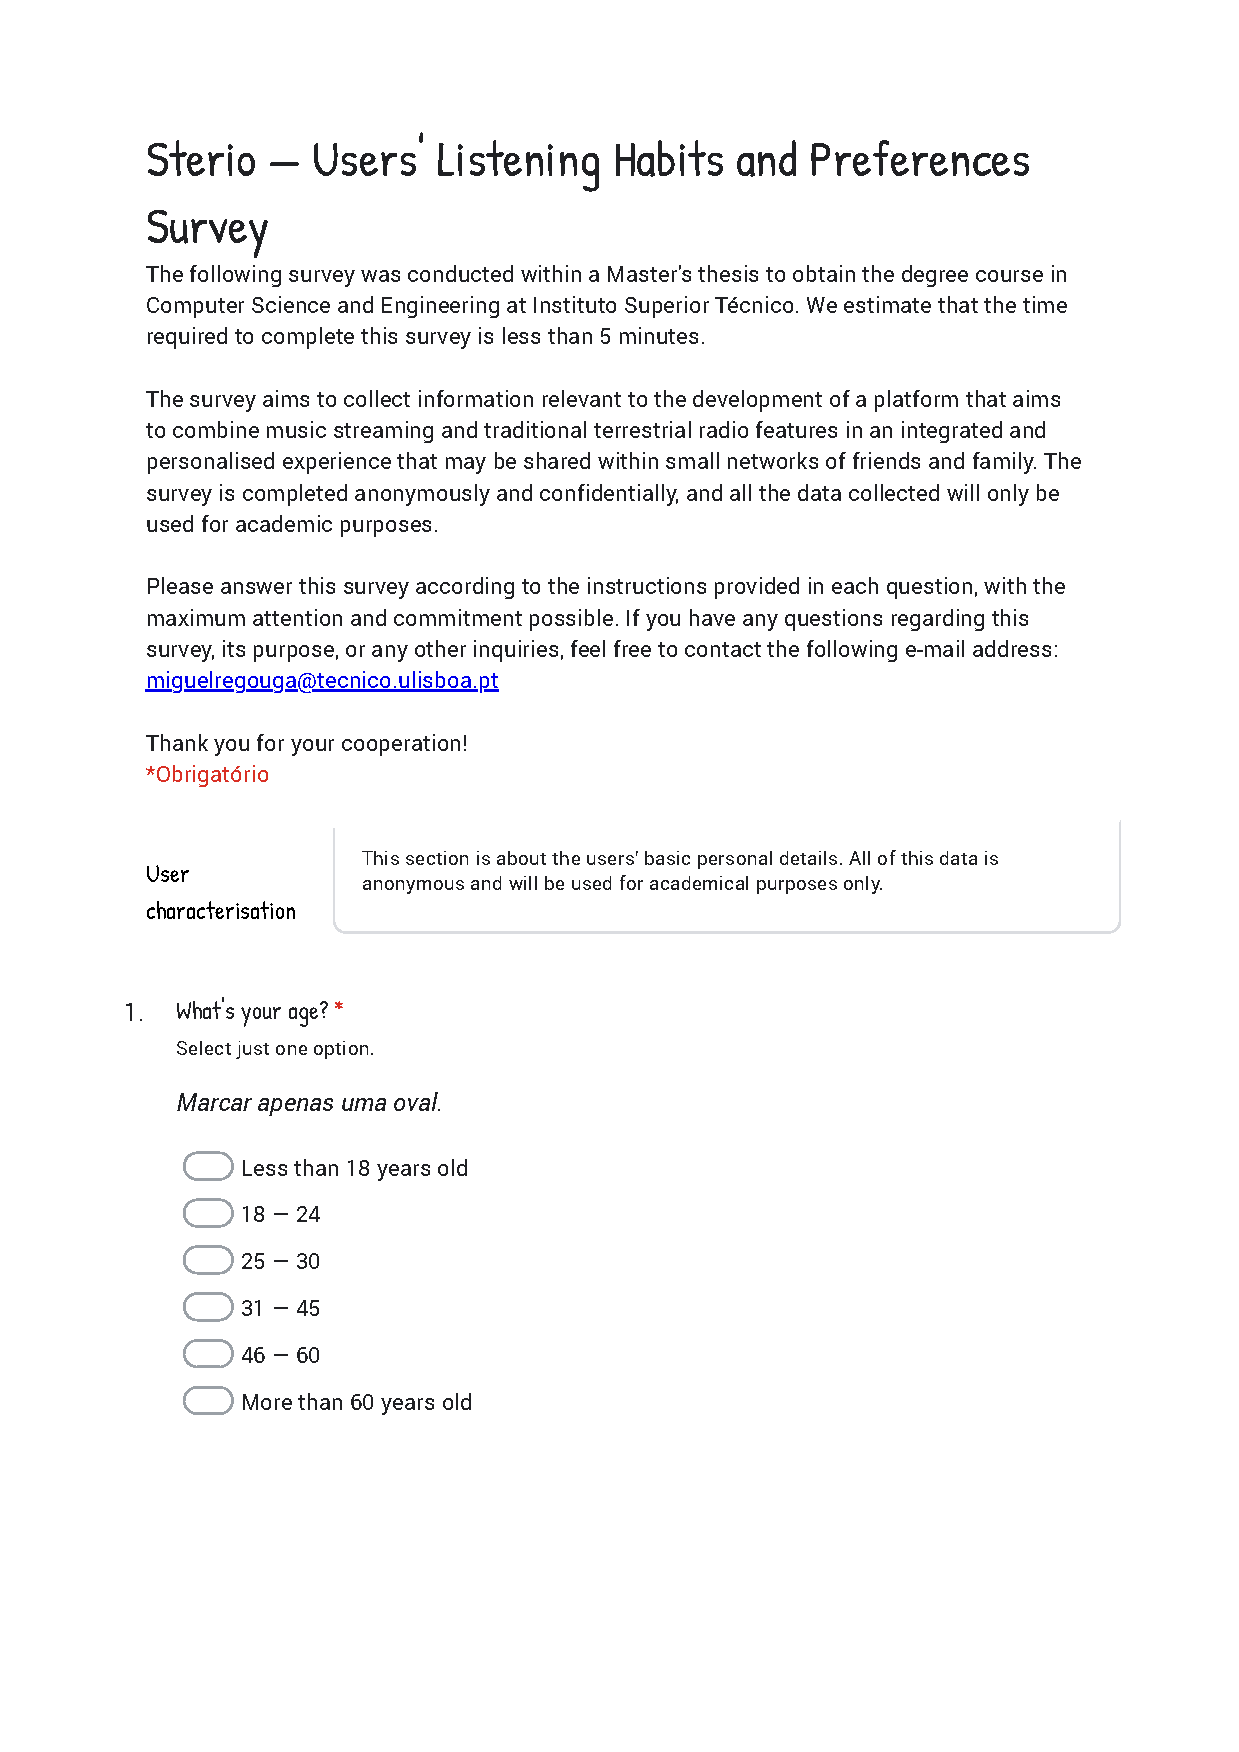
\includepdf[pages=-]{./appendix/Survey.pdf}

% #############################################################################

\chapter{Diary Study — Template}
\label{chapter:appendixB}

In this appendix, we present the template spreadsheet used for the diary study in the ambit of the preliminary user research. The filling of this template was conducted by each participant of the study using the Google Sheets platform.

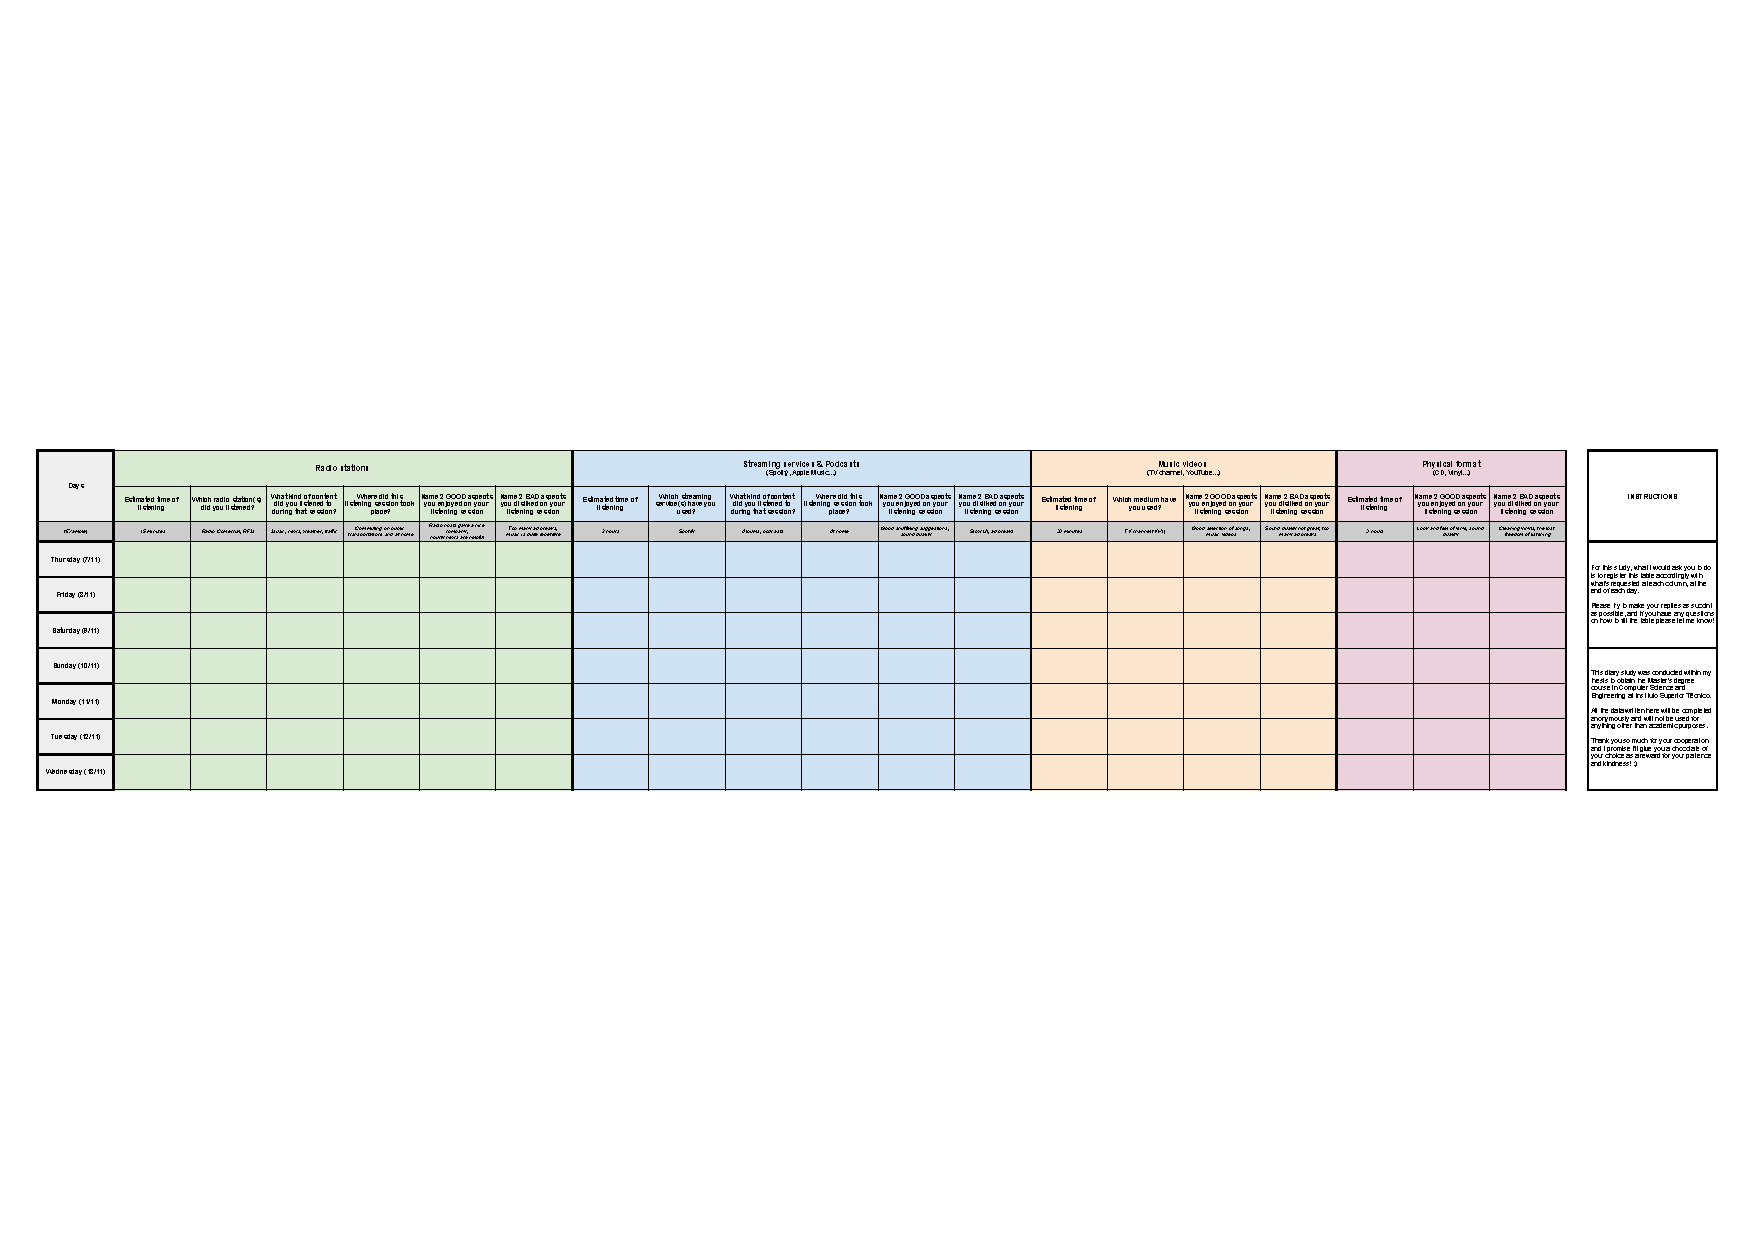
\includepdf[pages=-]{./appendix/dst.pdf}

% #############################################################################
\chapter{Diary Study — Informed Consent Form}
\label{chapter:appendixC}

In this appendix, we present the informed consent form users had to sign to participate in the diary study research activity.

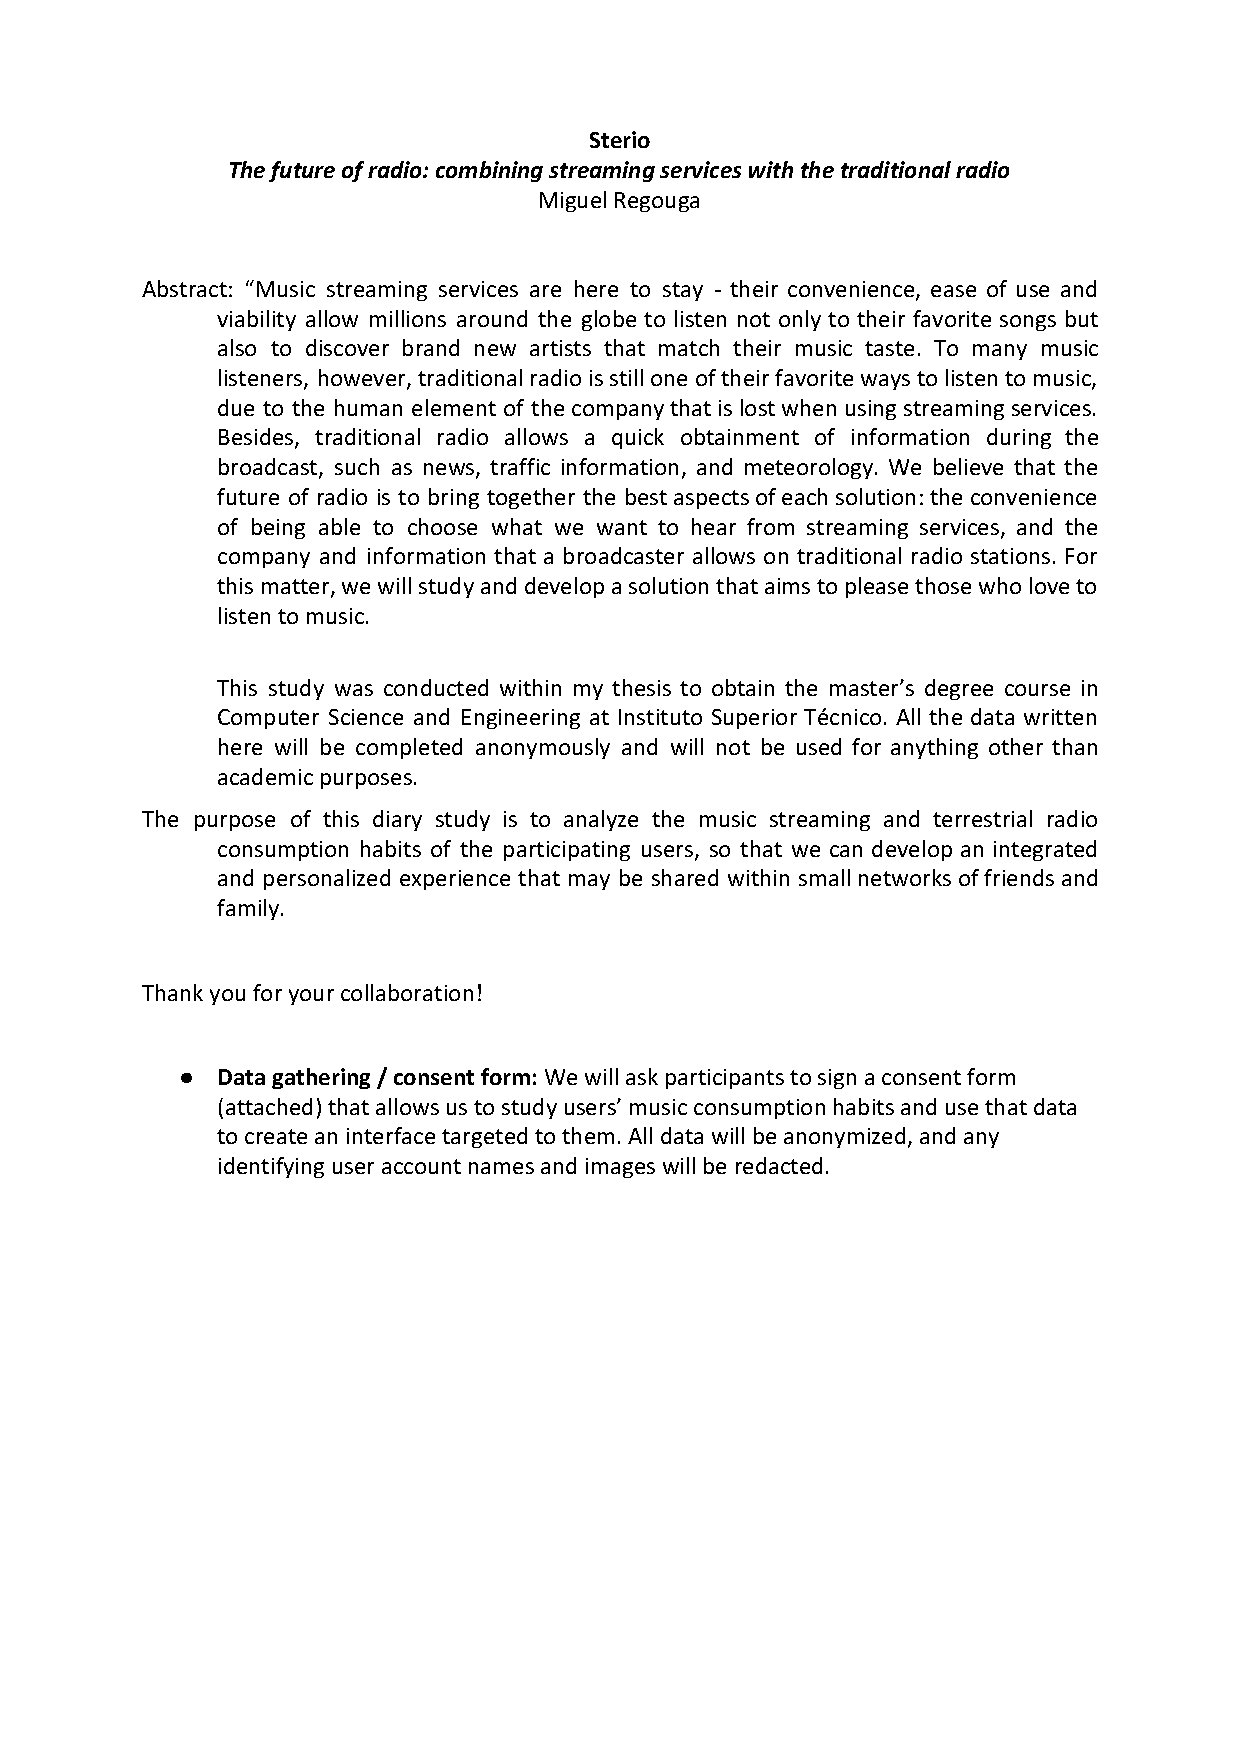
\includepdf[pages=-]{./appendix/dscf.pdf}

% #############################################################################
\chapter{Interview Guide}
\label{chapter:appendixD}

In this appendix, we present the followed guide for the follow-up interviews conducted with the participants of the diary study.

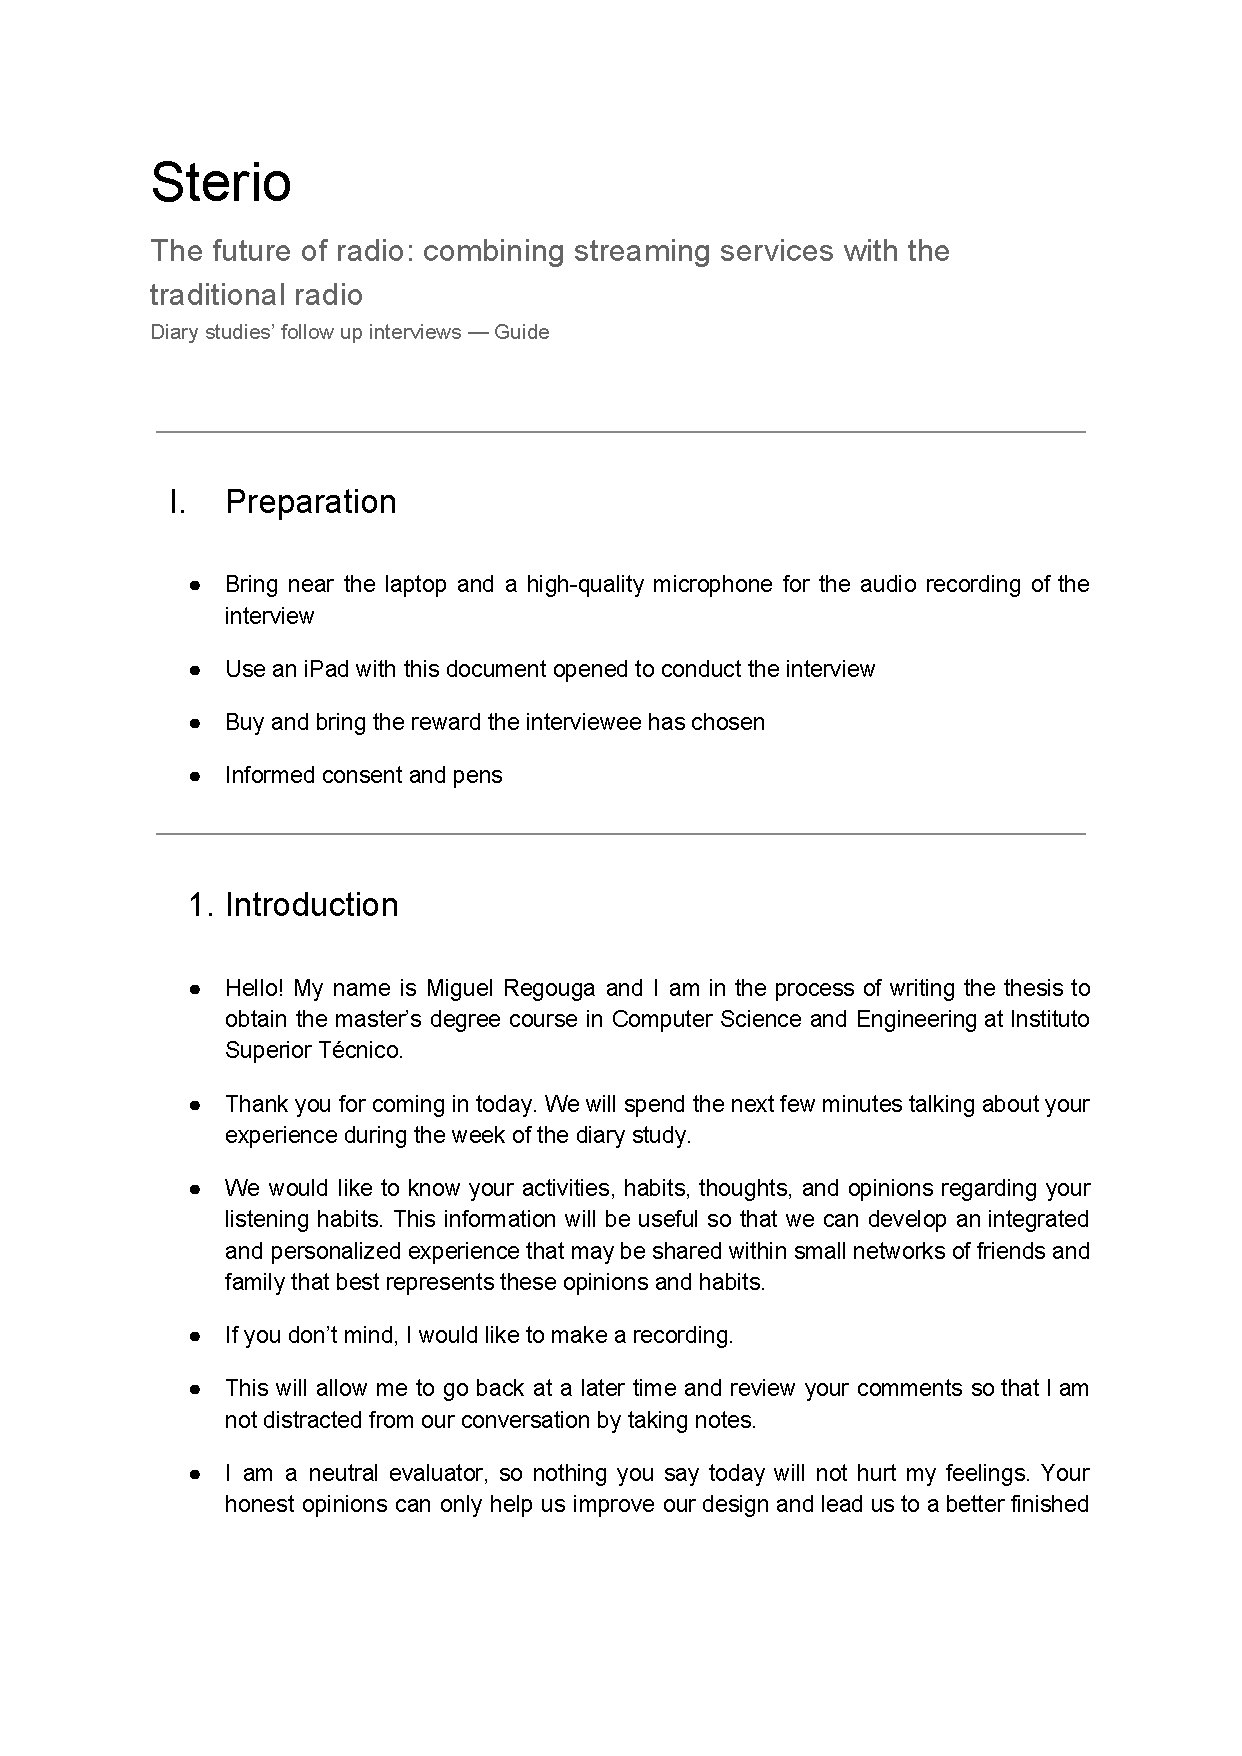
\includepdf[pages=-]{./appendix/Interview.pdf}



% #############################################################################
\chapter{Speed Dating — Need Validation Guide}
\label{chapter:appendixF}

In this appendix, we present the followed guide for the sessions conducted in the ambit of the need validation component of the speed dating methodology.


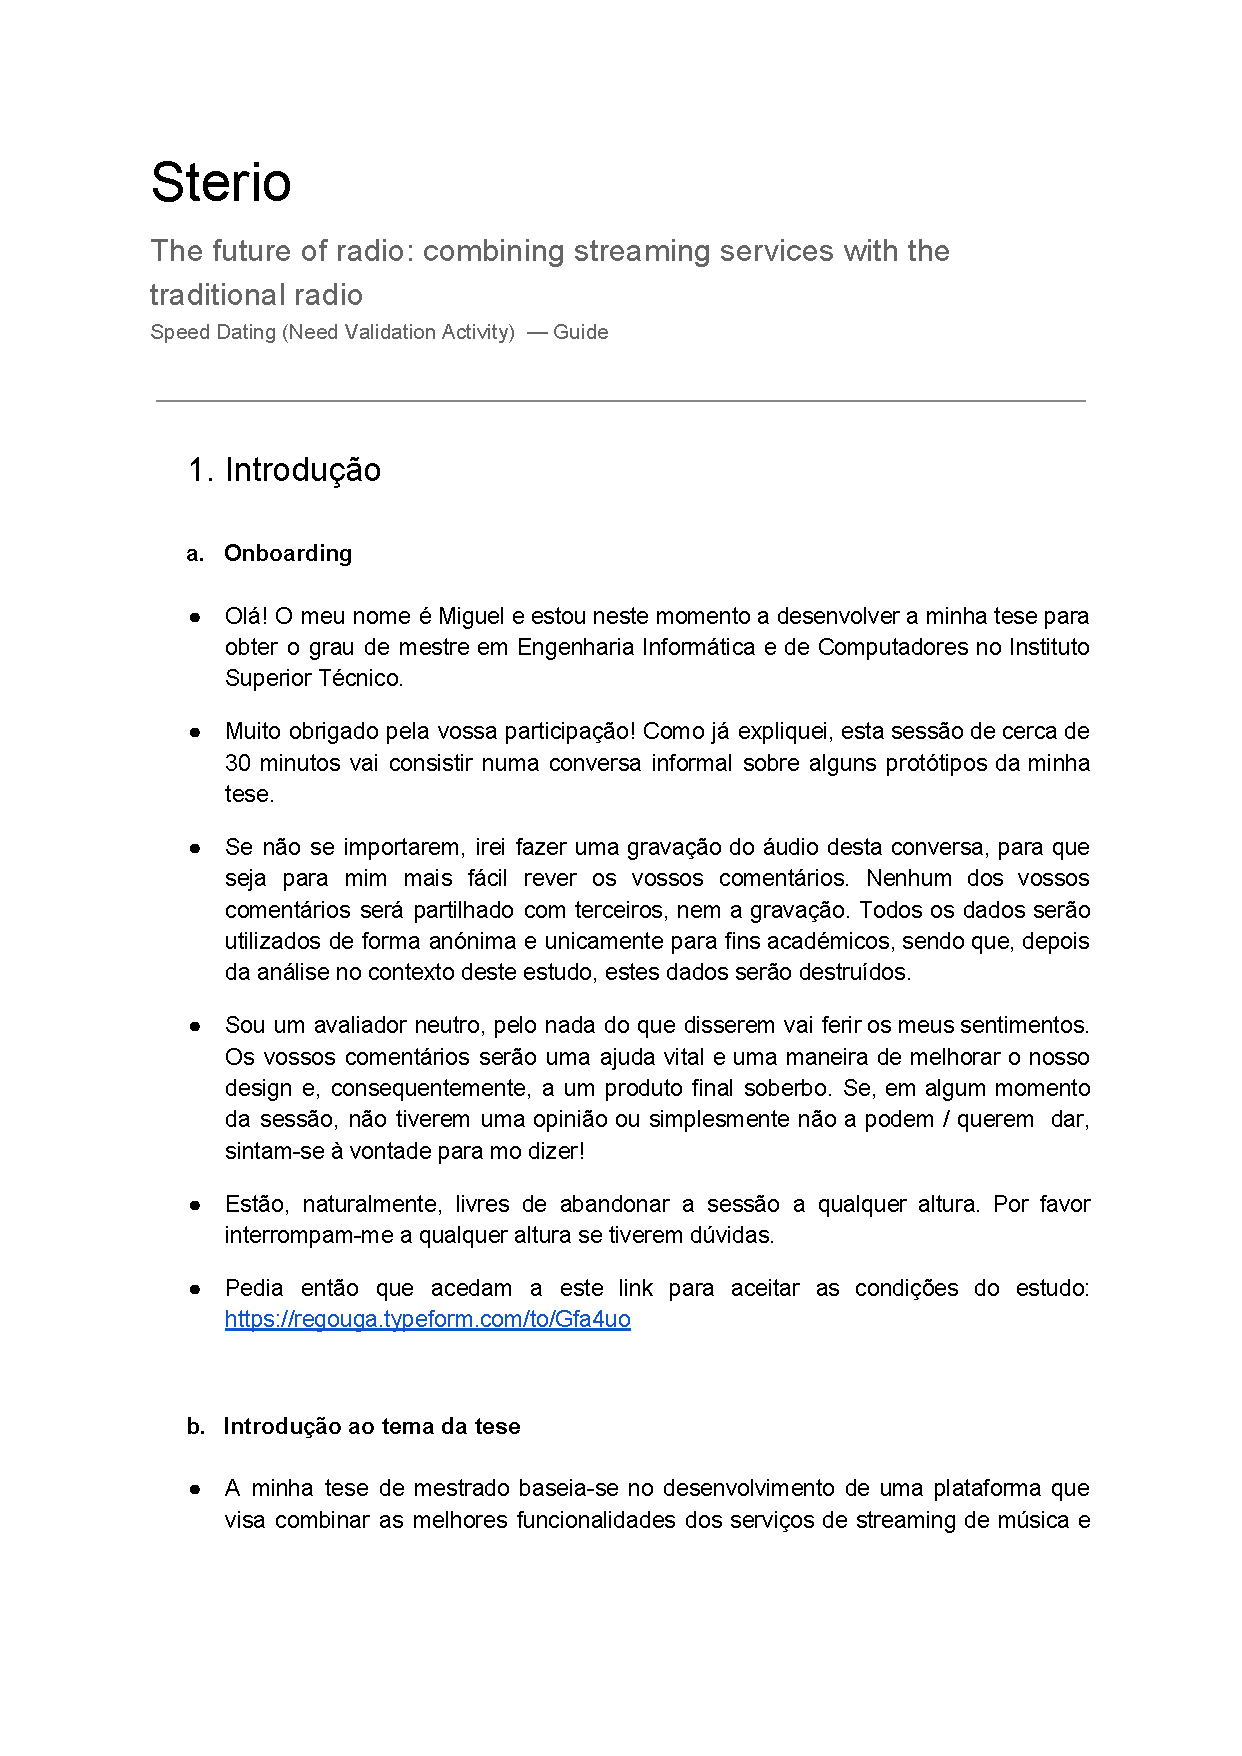
\includepdf[pages=-]{./appendix/nvg.pdf}

% #############################################################################
\chapter{Speed Dating — Need Validation Report}
\label{chapter:appendixG}

In this appendix, we present our procedures and reached conclusions of the need validation component of the speed dating methodology.

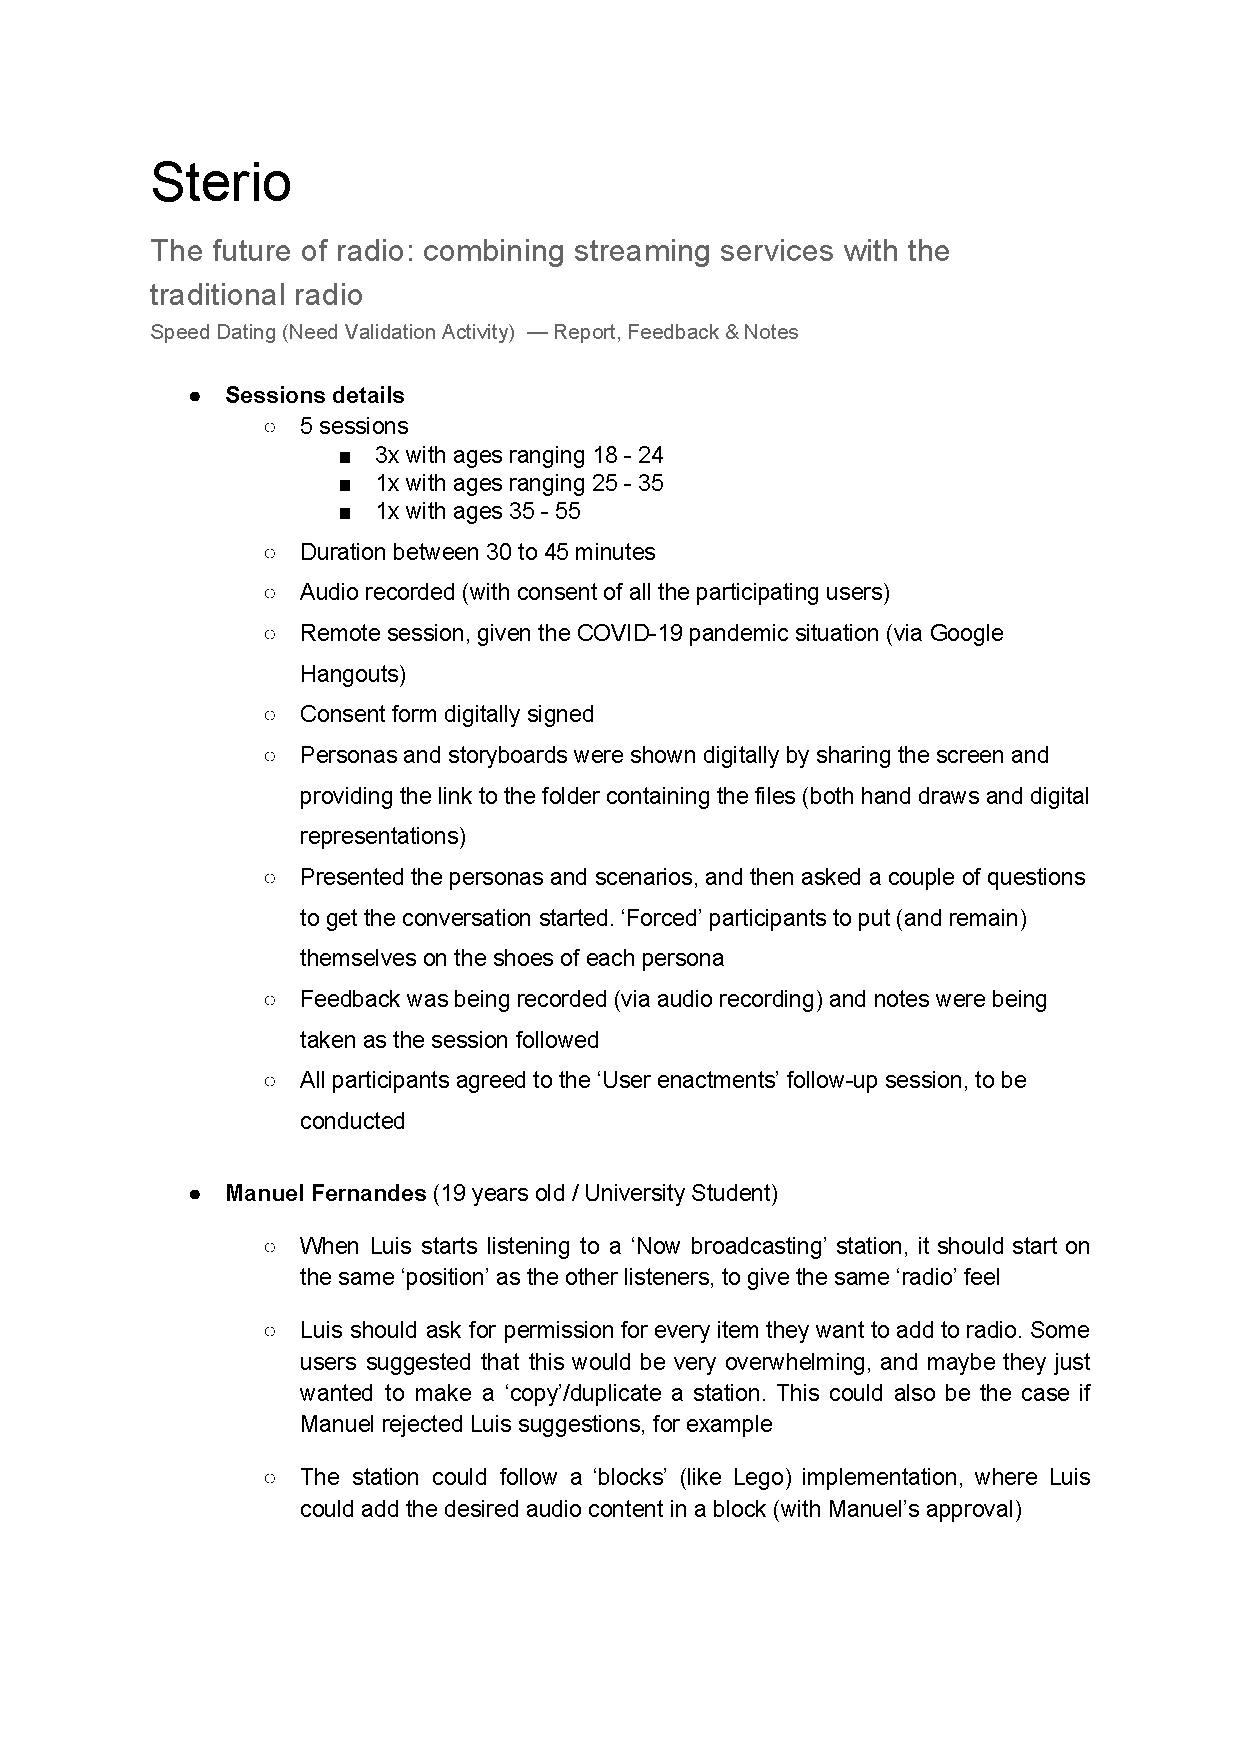
\includepdf[pages=-]{./appendix/nvr.pdf}

% #############################################################################
\chapter{Speed Dating — User Enactments Report}
\label{chapter:appendixE}

In this appendix, we present our procedures and reached conclusions of the user enactments component of the speed dating methodology.

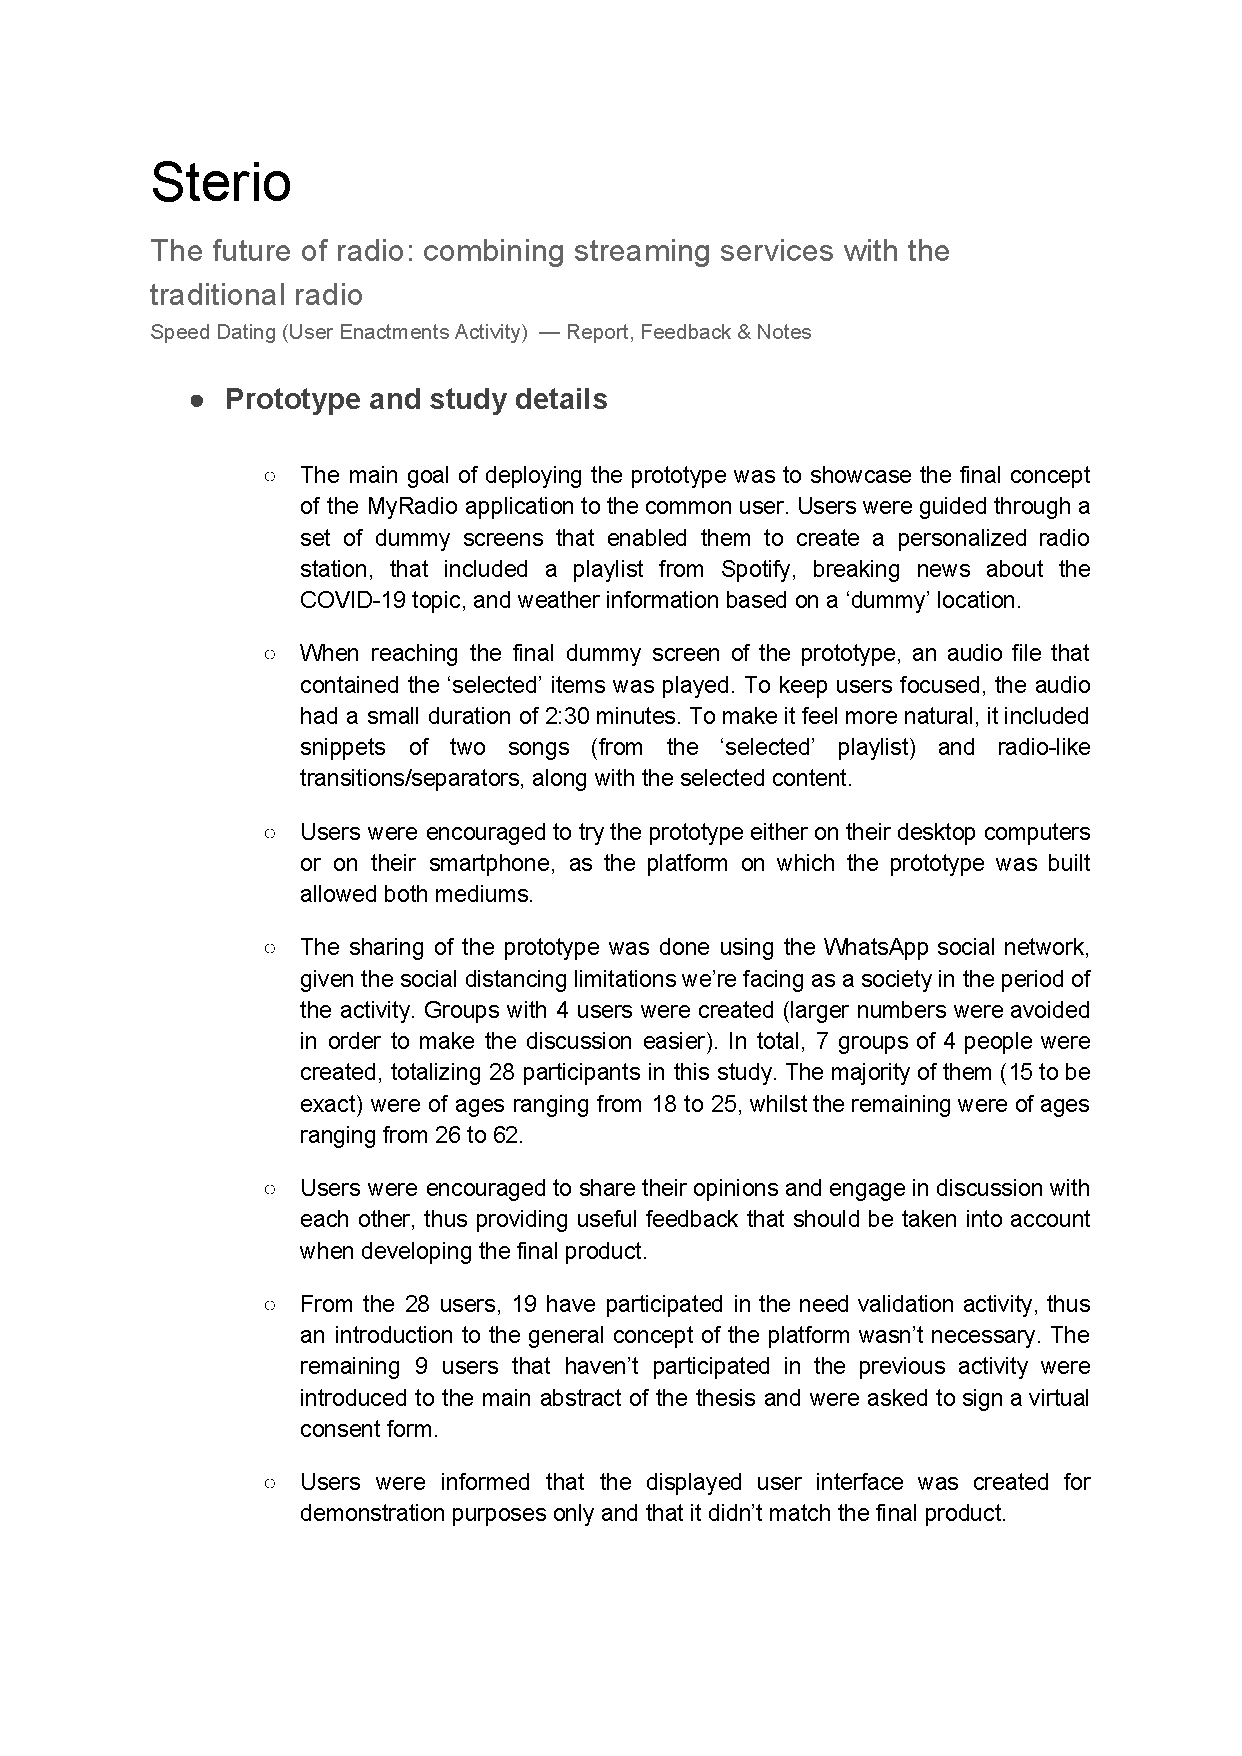
\includepdf[pages=-]{./appendix/uer.pdf}

% #############################################################################
\chapter{Usability Testing — Protocol}
\label{chapter:appendixH}

This appendix presents the usability tests script that should be followed by the test facilitator with every user.

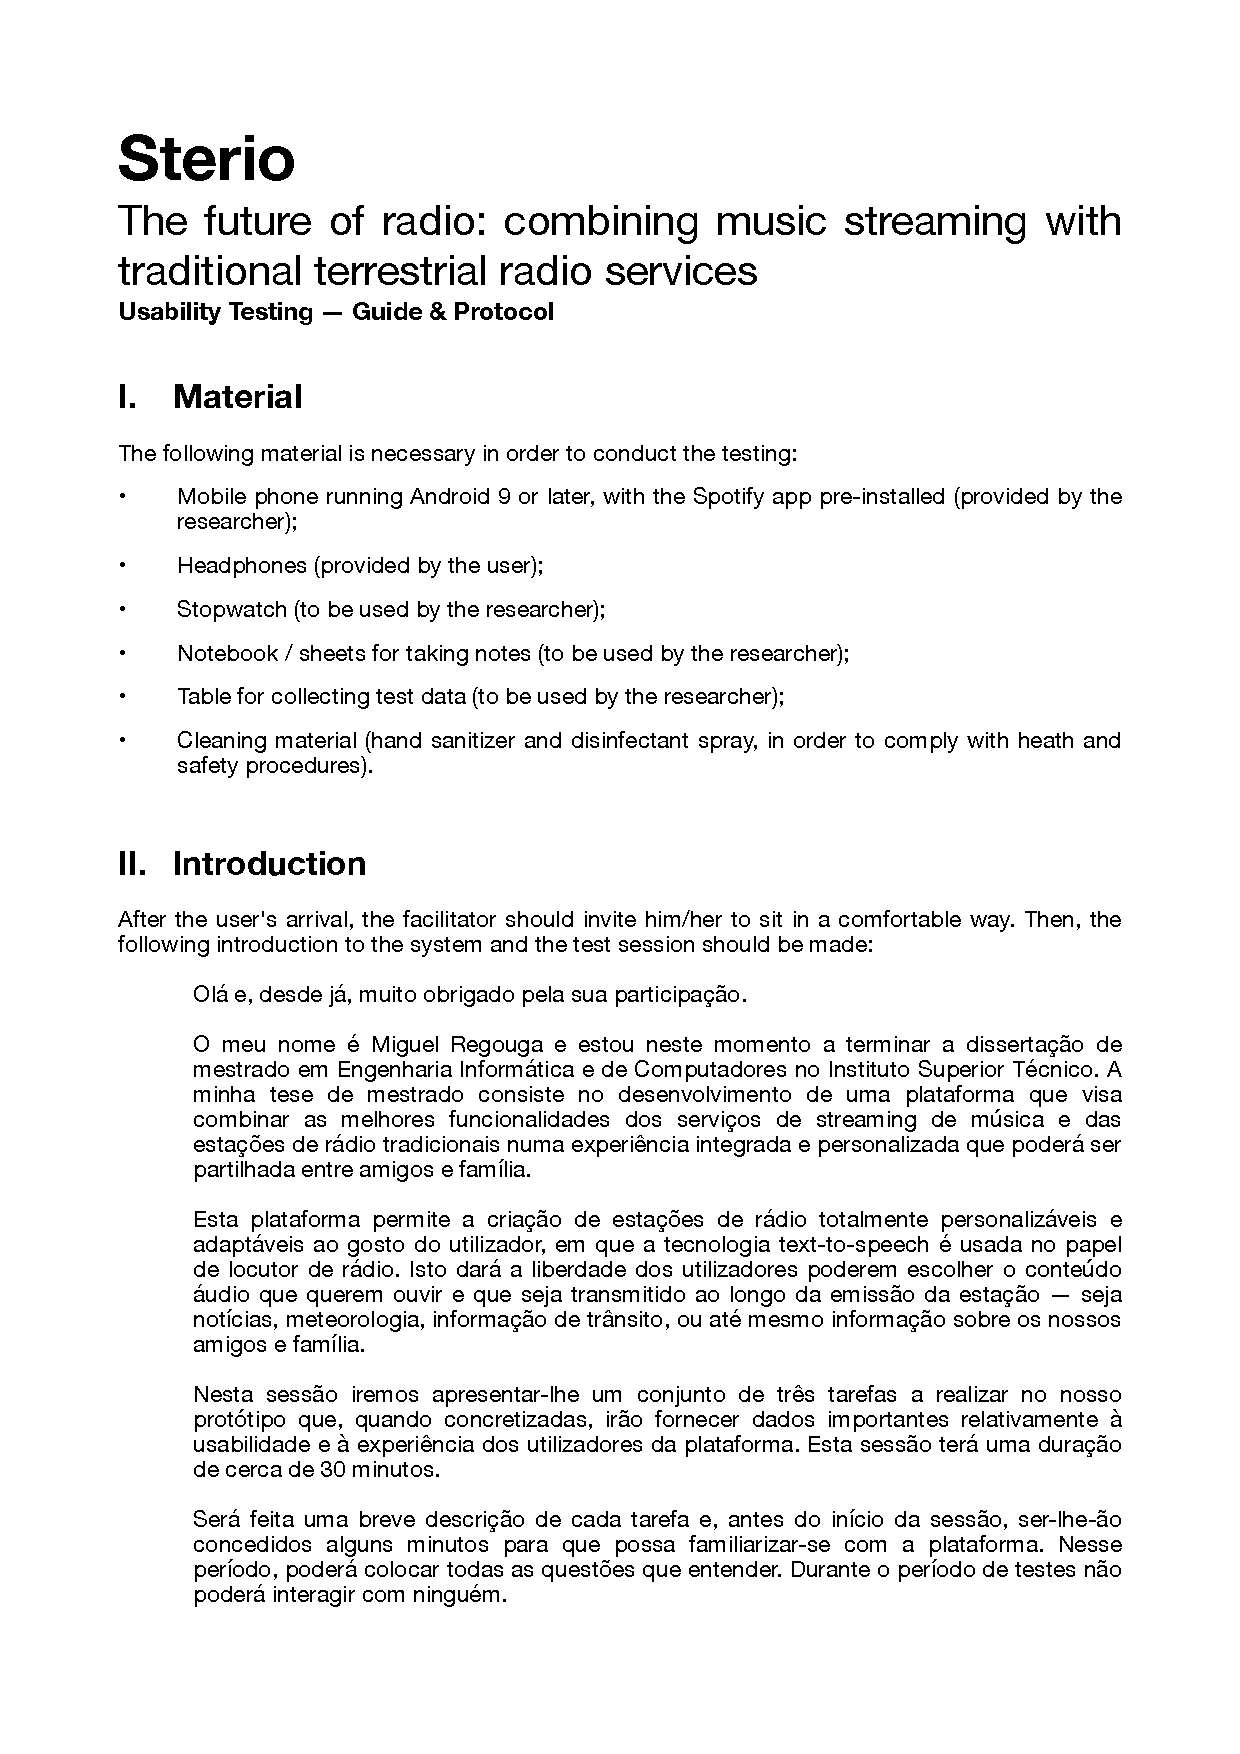
\includepdf[pages=-]{./appendix/utp.pdf}

% #############################################################################
\chapter{Usability Testing — Consent Form}
\label{chapter:appendixI}

In this appendix, we present the informed consent form users had to sign to participate in the usability testing sessions.

\includepdf[pages=-]{./appendix/cf.pdf}

% #############################################################################
\chapter{Usability Testing — Initial Survey}
\label{chapter:appendixJ}

In this appendix, we present the form used to collect demographic data about users that participated in usability tests.

\includepdf[pages=-]{./appendix/is.pdf}

% #############################################################################
\chapter{Usability Testing — Post-Task Survey}
\label{chapter:appendixK}


In this appendix, we present the form used to collect quantitative data regarding the performance of a given task of the usability tests.

\includepdf[pages=-]{./appendix/pt.pdf}

% #############################################################################
\chapter{Usability Testing — Final Survey}
\label{chapter:appendixL}

In this appendix, we present the form used to collect final quantitative and qualitative data in the ambit of the usability testing procedures.

\includepdf[pages=-]{./appendix/final.pdf}

% #############################################################################
\chapter{UbiComp/ISWC 2020 Poster}
\label{chapter:appendixM}

In this appendix, we present the submitted poster that was presented at UbiComp/ISWC 2020.

\includepdf[pages=-]{./appendix/poster.pdf}


%% If Printing on DOUBLE SIDED pages, the second page should be white.
%% Otherwise, comment the following command:
\cleardoublepage
%% Second Appendix
\pdfbookmark[1]{Appendix B}{appendix}
% #############################################################################
% This is Appendix B
% !TEX root = ../main.tex
% #############################################################################
\chapter{A Large Table}
\label{chapter:appendixB}

Aliquam et nisl vel ligula consectetuer suscipit. Morbi euismod enim eget neque. Donec sagittis massa. Vestibulum quis augue sit amet ipsum laoreet pretium. Nulla facilisi. Duis tincidunt, felis et luctus placerat, ipsum libero vestibulum sem, vitae elementum wisi ipsum a metus. Nulla a enim sed dui hendrerit lobortis. Donec lacinia vulputate magna. Vivamus suscipit lectus at quam. In lectus est, viverra a, ultricies ut, pulvinar vitae, tellus. Donec et lectus et sem rutrum sodales. Morbi cursus. Aliquam a odio. Sed tortor velit, convallis eget, porta interdum, convallis sed, tortor. Phasellus ac libero a lorem auctor mattis. Lorem ipsum dolor sit amet, consectetuer adipiscing elit.

Nunc auctor bibendum eros. Maecenas porta accumsan mauris. Etiam enim enim, elementum sed, bibendum quis, rhoncus non, metus. Fusce neque dolor, adipiscing sed, consectetuer et, lacinia sit amet, quam. Suspendisse wisi quam, consectetuer in, blandit sed, suscipit eu, eros. Etiam ligula enim, tempor ut, blandit nec, mollis eu, lectus. Nam cursus. Vivamus iaculis. Aenean risus purus, pharetra in, blandit quis, gravida a, turpis. Donec nisl. Aenean eget mi. Fusce mattis est id diam. Phasellus faucibus interdum sapien. Duis quis nunc. Sed enim.
Nunc auctor bibendum eros. Maecenas porta accumsan mauris. Etiam enim enim, elementum sed, bibendum quis, rhoncus non, metus. Fusce neque dolor, adipiscing sed, consectetuer et, lacinia sit amet, quam.

% Table Example
\newcommand{\greyrow}{\rowcolor[rgb]{0.9,0.9,0.9}}
\newcommand{\whiterow}{\rowcolor[rgb]{1,1,1}}
\newcommand{\greycell}[1]{\multicolumn{1}{{>{\columncolor[rgb]{0.9,0.9,0.9}}c}}{#1}}
\newcommand{\lightgreycell}[1]{\multicolumn{1}{{>{\columncolor[rgb]{0.9,0.9,0.9}}c}}{#1}}
\newcommand{\mediumgreycell}[1]{\multicolumn{1}{{>{\columncolor[rgb]{0.8,0.8,0.8}}c}}{#1}}
\newcommand{\darkgreycell}[1]{\multicolumn{1}{{>{\columncolor[rgb]{0.7,0.7,0.7}}c}}{#1}}
\newcommand{\whitecell}[1]{\multicolumn{1}{{>{\columncolor[rgb]{1,1,1}}c}}{#1}}

\newcommand{\cellformatG}[1]{\multicolumn{1}{{>{\columncolor[rgb]{.9,.9,.9}}c}}{#1}}
\newcommand{\cellformatW}[1]{\multicolumn{1}{{>{\columncolor[rgb]{1,1,1}}c}}{#1}}
\newcommand{\cellformatlG}[1]{\multicolumn{1}{{|>{\columncolor[rgb]{.9,.9,.9}}c}}{#1}}
\newcommand{\cellformatlW}[1]{\multicolumn{1}{{|>{\columncolor[rgb]{1,1,1}}c}}{#1}}
\newcommand{\cellformatrG}[1]{\multicolumn{1}{{>{\columncolor[rgb]{.9,.9,.9}}c|}}{#1}}
\newcommand{\cellformatrW}[1]{\multicolumn{1}{{>{\columncolor[rgb]{1,1,1}}c|}}{#1}}
\newcommand{\cellformatlrG}[1]{\multicolumn{1}{{|>{\columncolor[rgb]{.9,.9,.9}}c|}}{#1}}
\newcommand{\cellformatlrW}[1]{\multicolumn{1}{{|>{\columncolor[rgb]{1,1,1}}c|}}{#1}}

\begin{table}[t]
\centering
\caption{Example table}
\label{table:table1}
\begin{tabular}{c c c c c c}
\hline
\cellformatrG{}&\cellformatlG{}&\cellformatrG{}&\cellformatlG{}&\cellformatrG{}&\cellformatlG{}\\
\cellformatrG{}&
\cellformatlG{\multirow{-2}{*}{\centering\bf \#Layers}} & 
\cellformatrG{\multirow{-2}{*}{\centering\bf \#Nets}} & 
\cellformatlG{\multirow{-2}{*}{\centering \#Nodes\Mark1}} & 
\cellformatrG{\multirow{-2}{1.8cm}{\centering Critical path}}&
\cellformatlG{\multirow{-2}{2cm}{\centering\bf Latency ($T_{iter}$)}}\\
\cellformatrG{\multirow{-3}{2.2cm}{\centering Benchmark: ANN}} &
\cellformatlG{\footnotesize $(1)$} & 
\cellformatrG{\footnotesize$(2)$} & 
\cellformatlG{\footnotesize$(3)=8\cdot(1)\cdot(2)$} & 
\cellformatrG{\footnotesize$(4)=4\cdot(1)$} & 
\cellformatlG{\footnotesize$(5)$}\\
\hline
\cellformatrW{A1} & \cellformatlW{\bf 3--1501} & \cellformatrW{       1   } & \cellformatlW{\bf 24--12008}  & \cellformatrW{\bf 12--6004} & \cellformatlW{    4}\\
\cellformatrW{A2} & \cellformatlW{    501    } & \cellformatrW{       1   } & \cellformatlW{     4008    }  & \cellformatrW{  2004      } & \cellformatlW{\bf 2--2000 }\\
\cellformatrW{A3} & \cellformatlW{     10    } & \cellformatrW{\bf 2--1024} & \cellformatlW{\bf 160--81920} & \cellformatrW{    40      } & \cellformatlW{   60\Mark2 }\\
\cellformatrW{A4} & \cellformatlW{     10    } & \cellformatrW{      50   } & \cellformatlW{     4000    }  & \cellformatrW{    40      } & \cellformatlW{\bf 80--1200}\\
\hline
\multicolumn{6}{c}{\vspace*{-0.3cm}}\\
%%%%%%%%%%%%% SECOND PART OF THE TABLE %%%%%%%%%%%%%%%%%%%%%%%%
\hline
\cellformatrG{}&\cellformatlG{}&\cellformatrG{}&\cellformatlG{}&\cellformatrG{}&\cellformatlG{}\\
\cellformatrG{}&
\cellformatlG{\multirow{-2}{1.6cm}{\centering\bf FFT size\Mark3}} & 
\cellformatrG{\multirow{-2}{*}{\centering\it\#Inputs}} & 
\cellformatlG{\multirow{-2}{*}{\centering\it \#Nodes\Mark1}} & 
\cellformatrG{\multirow{-2}{1.8cm}{\centering\it Critical path}}&
\cellformatlG{\multirow{-2}{2cm}{\centering\bf Latency ($T_{iter}$)}}\\
\cellformatrG{\multirow{-3}{2.2cm}{\centering Benchmark: FFT}}& 
\cellformatlG{\footnotesize$(1)$} & 
\cellformatrG{\footnotesize$(2)=2^{(1)}$} & 
\cellformatlG{\footnotesize$(3)=10\cdot(1)\cdot (2)$} & 
\cellformatrG{\footnotesize$(4)=4\cdot (1)$} & 
\cellformatlG{\footnotesize$(5)$}\\
\hline
\cellformatrW{F1} & \cellformatlW{\bf 1--10} & \cellformatrW{2--1024} & \cellformatlW{\bf 20--102400} &  \cellformatrW{4--40} & \cellformatlW{6--60\Mark2}\\
\cellformatrW{F2} & \cellformatlW{\bf 5} & \cellformatrW{32} & \cellformatlW{1600} & \cellformatrW{20} & \cellformatlW{\bf 40 -- 1500}\\
\hline
\multicolumn{6}{c}{\vspace*{-0.3cm}}\\
% THIRD AND LAST TABLE!!!
\hline
\cellformatrG{}&\cellformatlG{}&\cellformatrG{}&\cellformatlG{}&\cellformatrG{}&\cellformatlG{}\\
\cellformatrG{}&
\cellformatlG{\multirow{-2}{*}{\centering\bf\#Types}} & 
\cellformatrG{\multirow{-2}{*}{\centering\bf \#Nodes}} & 
\cellformatlG{\multirow{-2}{*}{\centering\it \#Networks}} & 
\cellformatrG{\multirow{-2}{1.8cm}{\centering\it Critical path}}&
\cellformatlG{\multirow{-2}{2cm}{\centering\bf Latency ($T_{iter}$)}}\\
\cellformatrG{\multirow{-3}{2.2cm}{\centering Benchmark: Random networks}}& 
\cellformatlG{\footnotesize$(1)$} & 
\cellformatrG{\footnotesize$(2)$} & 
\cellformatlG{\footnotesize$(3)$} &
\cellformatrG{\footnotesize$(4)$} & 
\cellformatlG{\footnotesize$(5)$}\\
\hline
\cellformatrW{R1} & \cellformatlW{3} & \cellformatrW{10--2000} & \cellformatlW{500} &  \cellformatrW{\it variable} & \cellformatlW{\footnotesize$(4)$}\\
\cellformatrW{R2} & \cellformatlW{3} & \cellformatrW{  50    } & \cellformatlW{500} &  \cellformatrW{\it variable} & \cellformatlW{\footnotesize$(4)\times [1;\cdots;20]$}\\
\hline
\multicolumn{6}{c}{\vspace*{-0.3cm}}\\
\multicolumn{6}{l}{\it\Mark1 Excluding constant nodes.}\\
\multicolumn{6}{l}{\it\Mark2 Value kept proportional to the critical path: $(5)=(4)*1.5$.}\\
\multicolumn{6}{l}{\it\Mark3 A size of $x$ corresponds to a $2^x$ point FFT.}\\
\multicolumn{6}{l}{\it Values in bold indicate the parameter being varied.}
\end{tabular}
\end{table}

\textcolor{violet}{As \Cref{table:table1} shows, the data can be inserted from a file, in the case of a somehow complex structure. Notice the Table footnotes.}	

Lorem ipsum dolor sit amet, consectetuer adipiscing elit. Morbi commodo, ipsum sed pharetra gravida, orci magna rhoncus neque, id pulvinar odio lorem non turpis. Nullam sit amet enim. Suspendisse id velit vitae ligula volutpat condimentum. Aliquam erat volutpat. Sed quis velit. Nulla facilisi. Nulla libero. Vivamus pharetra posuere sapien. Nam consectetuer. Sed aliquam, nunc eget euismod ullamcorper, lectus nunc ullamcorper orci, fermentum bibendum enim nibh eget ipsum. Donec porttitor ligula eu dolor. Maecenas vitae nulla consequat libero cursus venenatis. Nam magna enim, accumsan eu, blandit sed, blandit a, eros. 

\textcolor{violet}{And now an example (\Cref{tab:lon_table}) of a table that extends to more than one page. Notice the repetition of the Caption (with indication that is continued) and of the Header, as well as the continuation text at the bottom.}

\begin{center}
\begin{longtable}{|l|l|l|}
\caption[Example of a very long table spreading in several pages]{Example of a very long table spreading in several pages} \label{tab:lon_table} \\

\hline \multicolumn{1}{|c|}{\textbf{Time (s)}} & \multicolumn{1}{c|}{\textbf{Triple chosen}} & \multicolumn{1}{c|}{\textbf{Other feasible triples}} \\ \hline 
\endfirsthead

\multicolumn{3}{c}%
{{\bfseries \tablename\ \thetable{} -- continued from previous page}} \\
\hline \multicolumn{1}{|c|}{\textbf{Time (s)}} &
\multicolumn{1}{c|}{\textbf{Triple chosen}} &
\multicolumn{1}{c|}{\textbf{Other feasible triples}} \\ \hline 
\endhead

\hline \multicolumn{3}{|r|}{{Continued on next page}} \\ \hline
\endfoot

\hline \hline
\endlastfoot
0 & (1, 11, 13725) & (1, 12, 10980), (1, 13, 8235), (2, 2, 0), (3, 1, 0) \\
2745 & (1, 12, 10980) & (1, 13, 8235), (2, 2, 0), (2, 3, 0), (3, 1, 0) \\
5490 & (1, 12, 13725) & (2, 2, 2745), (2, 3, 0), (3, 1, 0) \\
8235 & (1, 12, 16470) & (1, 13, 13725), (2, 2, 2745), (2, 3, 0), (3, 1, 0) \\
10980 & (1, 12, 16470) & (1, 13, 13725), (2, 2, 2745), (2, 3, 0), (3, 1, 0) \\
13725 & (1, 12, 16470) & (1, 13, 13725), (2, 2, 2745), (2, 3, 0), (3, 1, 0) \\
16470 & (1, 13, 16470) & (2, 2, 2745), (2, 3, 0), (3, 1, 0) \\
19215 & (1, 12, 16470) & (1, 13, 13725), (2, 2, 2745), (2, 3, 0), (3, 1, 0) \\
21960 & (1, 12, 16470) & (1, 13, 13725), (2, 2, 2745), (2, 3, 0), (3, 1, 0) \\
24705 & (1, 12, 16470) & (1, 13, 13725), (2, 2, 2745), (2, 3, 0), (3, 1, 0) \\
27450 & (1, 12, 16470) & (1, 13, 13725), (2, 2, 2745), (2, 3, 0), (3, 1, 0) \\
30195 & (2, 2, 2745) & (2, 3, 0), (3, 1, 0) \\
32940 & (1, 13, 16470) & (2, 2, 2745), (2, 3, 0), (3, 1, 0) \\
35685 & (1, 13, 13725) & (2, 2, 2745), (2, 3, 0), (3, 1, 0) \\
38430 & (1, 13, 10980) & (2, 2, 2745), (2, 3, 0), (3, 1, 0) \\
41175 & (1, 12, 13725) & (1, 13, 10980), (2, 2, 2745), (2, 3, 0), (3, 1, 0) \\
43920 & (1, 13, 10980) & (2, 2, 2745), (2, 3, 0), (3, 1, 0) \\
46665 & (2, 2, 2745) & (2, 3, 0), (3, 1, 0) \\
49410 & (2, 2, 2745) & (2, 3, 0), (3, 1, 0) \\
52155 & (1, 12, 16470) & (1, 13, 13725), (2, 2, 2745), (2, 3, 0), (3, 1, 0) \\
54900 & (1, 13, 13725) & (2, 2, 2745), (2, 3, 0), (3, 1, 0) \\
57645 & (1, 13, 13725) & (2, 2, 2745), (2, 3, 0), (3, 1, 0) \\
60390 & (1, 12, 13725) & (2, 2, 2745), (2, 3, 0), (3, 1, 0) \\
63135 & (1, 13, 16470) & (2, 2, 2745), (2, 3, 0), (3, 1, 0) \\
65880 & (1, 13, 16470) & (2, 2, 2745), (2, 3, 0), (3, 1, 0) \\
68625 & (2, 2, 2745) & (2, 3, 0), (3, 1, 0) \\
71370 & (1, 13, 13725) & (2, 2, 2745), (2, 3, 0), (3, 1, 0) \\
74115 & (1, 12, 13725) & (2, 2, 2745), (2, 3, 0), (3, 1, 0) \\
76860 & (1, 13, 13725) & (2, 2, 2745), (2, 3, 0), (3, 1, 0) \\
79605 & (1, 13, 13725) & (2, 2, 2745), (2, 3, 0), (3, 1, 0) \\
82350 & (1, 12, 13725) & (2, 2, 2745), (2, 3, 0), (3, 1, 0) \\
85095 & (1, 12, 13725) & (1, 13, 10980), (2, 2, 2745), (2, 3, 0), (3, 1, 0) \\
87840 & (1, 13, 16470) & (2, 2, 2745), (2, 3, 0), (3, 1, 0) \\
90585 & (1, 13, 16470) & (2, 2, 2745), (2, 3, 0), (3, 1, 0) \\
93330 & (1, 13, 13725) & (2, 2, 2745), (2, 3, 0), (3, 1, 0) \\
96075 & (1, 13, 16470) & (2, 2, 2745), (2, 3, 0), (3, 1, 0) \\
98820 & (1, 13, 16470) & (2, 2, 2745), (2, 3, 0), (3, 1, 0) \\
101565 & (1, 13, 13725) & (2, 2, 2745), (2, 3, 0), (3, 1, 0) \\
104310 & (1, 13, 16470) & (2, 2, 2745), (2, 3, 0), (3, 1, 0) \\
107055 & (1, 13, 13725) & (2, 2, 2745), (2, 3, 0), (3, 1, 0) \\
109800 & (1, 13, 13725) & (2, 2, 2745), (2, 3, 0), (3, 1, 0) \\
112545 & (1, 12, 16470) & (1, 13, 13725), (2, 2, 2745), (2, 3, 0), (3, 1, 0) \\
115290 & (1, 13, 16470) & (2, 2, 2745), (2, 3, 0), (3, 1, 0) \\
118035 & (1, 13, 13725) & (2, 2, 2745), (2, 3, 0), (3, 1, 0) \\
120780 & (1, 13, 16470) & (2, 2, 2745), (2, 3, 0), (3, 1, 0) \\
123525 & (1, 13, 13725) & (2, 2, 2745), (2, 3, 0), (3, 1, 0) \\
126270 & (1, 12, 16470) & (1, 13, 13725), (2, 2, 2745), (2, 3, 0), (3, 1, 0) \\
129015 & (2, 2, 2745) & (2, 3, 0), (3, 1, 0) \\
131760 & (2, 2, 2745) & (2, 3, 0), (3, 1, 0) \\
134505 & (1, 13, 16470) & (2, 2, 2745), (2, 3, 0), (3, 1, 0) \\
137250 & (1, 13, 13725) & (2, 2, 2745), (2, 3, 0), (3, 1, 0) \\
139995 & (2, 2, 2745) & (2, 3, 0), (3, 1, 0) \\
142740 & (2, 2, 2745) & (2, 3, 0), (3, 1, 0) \\
145485 & (1, 12, 16470) & (1, 13, 13725), (2, 2, 2745), (2, 3, 0), (3, 1, 0) \\
148230 & (2, 2, 2745) & (2, 3, 0), (3, 1, 0) \\
150975 & (1, 13, 16470) & (2, 2, 2745), (2, 3, 0), (3, 1, 0) \\
153720 & (1, 12, 13725) & (2, 2, 2745), (2, 3, 0), (3, 1, 0) \\
156465 & (1, 13, 13725) & (2, 2, 2745), (2, 3, 0), (3, 1, 0) \\
159210 & (1, 13, 13725) & (2, 2, 2745), (2, 3, 0), (3, 1, 0) \\
161955 & (1, 13, 16470) & (2, 2, 2745), (2, 3, 0), (3, 1, 0) \\
164700 & (1, 13, 13725) & (2, 2, 2745), (2, 3, 0), (3, 1, 0) \\
\end{longtable}
\end{center}
%% If Printing on DOUBLE SIDED pages, the second page should be white.
%% Otherwise, comment the following command:
\cleardoublepage

% -----------------------------------------------------------------------------
% And this is THE END of the IST Thesis Document
\end{document}